%-------------------------------------------------------------------------------
%% outhesis_template.tex
%% version 1.0
%% Chris McRaven <mcraven@physics.ou.edu>
%%
%% 'outhesis.cls' is a class file for a master or phd thesis that
%% conforms to the requirements of the graduate college at the
%% University of Oklahoma. This file is a hacked version of 'book.cls,'
%% that includes all of the formatting requirements set forth in
%% the document 'DissertationInstPacket.pdf' available at
%% http://gradweb.ou.edu/Current/Forms/doctoral/DissertationPagination.pdf
%%
%% This class file relies on a few packages to work.  You must have the
%% following packages installed:
%%  amsfonts, amsmath, amssymb, tikz, lineno, microtype, hyperref
%%
%% Most of these packages are included in distributions of latex.  If you
%% get a lot of errors when compiling, check that these packages are
%% installed.
%%
%% By default, the class file will conform to the requirements, but three
%% options are provided for assistance in proofing the document.
%%
%% linenumbers -- turns on linenumbers in the left margin
%% summarypage -- places a page at the beginning of the document listing 
%%                the number of tables, figures, and bibliography items.
%% hyperlinks -- hyperlinks the citations and references for easier
%%                navigation in the document in a reader which supports
%%                hyperlinks.
%%
%-------------------------------------------------------------------------------

\newcommand*{\ATLASLATEXPATH}{atlas_latex/}

%\documentclass[linenumbers,summarypage,hyperlinks]{outhesis}
%\documentclass[linenumbers,hyperlinks]{outhesis}
\documentclass[hyperlinks]{outhesis}
%\documentclass{outhesis}



%-------------------------------------------------------------------------------
% Extra packages:
%-------------------------------------------------------------------------------
% See doc/atlas-physics.pdf for a list of the defined symbols.
% Default options are:
%   true:  journal, misc, particle, unit, xref
%   false: BSM, hion, math, process, other, texmf
% See the package for details on the options.

%\usepackage{\ATLASLATEXPATH atlasbiblatex} % Style file with biblatex options for ATLAS documents.
\usepackage{\ATLASLATEXPATH atlasphysics} % Useful macros
\usepackage[margin=1.0in]{geometry} % see geometry.pdf on how to lay out the page. There's lots.
%\usepackage{geometry} % see geometry.pdf on how to lay out the page. There's lots.
\usepackage{graphicx}
%\usepackage{subfigure} % obsolete. Use subcaption instead.
\usepackage{subcaption} %These packages gives the author the ability to have subfigures within figures, or subtables within table floats.
\usepackage[labelsep=colon,labelfont=bf,font=singlespacing,width=\textwidth,compatibility=false]{caption}
\usepackage{hyperref} % for url
\usepackage{slashed} % Dirac slash notation
\usepackage{amsmath}
\usepackage{authblk}
\usepackage{multirow}
\usepackage{booktabs} % enable the use of \toprule, \midrule, and \bottomrule
\usepackage{color} % for setting font color
\usepackage{bm} % bold and itatic in math mode


\geometry{a4paper} % or letter or a5paper or ... etc
% \geometry{landscape} % rotated page geometry

%\usepackage[english]{babel}
%\usepackage[utf8x]{inputenc}
%\usepackage{listings}
%\usepackage{textpos}  % for putting logo
%\usepackage{tikz}     % transparent background image
%\usepackage{eurosym}  % euro sign
%\usepackage{appendixnumberbeamer} % count presentation slides only
%\usepackage{pbox} % new line in cell of table
%\usepackage{tabularx} % can change the table width

%\newcommand{\HRule}{\rule{\linewidth}{0.3mm}}

%%%%%
%%%%%
%\usepackage[explicit]{titlesec}
%\usepackage{fix-cm}
%\usepackage{lipsum}
%% numbered
%\titleformat{\chapter}
%  {\normalfont\LARGE\bfseries\filleft}
%  {}
%  {0em}
%  {%
%    \parbox[b]{\dimexpr\linewidth-2.5cm\relax}{#1}\hfill%
%    \parbox[b]{2cm}{\hfill{\fontsize{80}{96}\selectfont\thechapter}}%
%  }
%% unnumbered
%\titleformat{name=\chapter,numberless}
%  {\normalfont\LARGE\bfseries\filleft}
%  {}
%  {0em}
%  {\parbox[b]{\dimexpr\linewidth-2.5cm\relax}{#1}}
%% spacing
%\titlespacing*{\chapter}
%  {0pt}{50pt}{40pt}
%%%%%
%%%%%  


%\usepackage[toc]{appendix}
%\usepackage{xspace}
%\usepackage{multirow,bigdelim}
%\usepackage[compat=1.1.0]{tikz-feynman}

% For a bibliography style, you must have the appropriate .bst file
% \bibliographystyle{apj}
%\bibliographystyle{prsty}
%\bibliographystyle{atlasBibStyleWithTitle}

%\usepackage{thesis-def}


%-------------------------------------------------------------------------------
% Content
%-------------------------------------------------------------------------------
 
%%% BEGIN DOCUMENT
\begin{document}

%% Place Dissertation information here
\author{Yu-Ting Shen}
\university{University of Oklahoma}
\college{Graduate College}
\department{Homer L. Dodge Department of Physics and Astronomy}
\title{This is the thesis title}
\address{Norman, Oklahoma}
\yr{2017}
\dgname{Doctor of Philosophy}
%% List your committee members here
\committee{{Dr. Patrick Skubic, Chair}, Dr. Michael Strauss, {Dr. Ron Kantowski}, Dr. Deborah Watson, {Dr. S. Lakshmivarahan}}

%% Put your dedication here. This is completely optional. Delete it if you don't need it.
\begin{dedication}
%To my past, present, and future family.
\begin{quotation}
\raggedright{\emph{`Blood, sweat \& respect. First two you give, last one you earn.''}} \\
\raggedleft{- Dwayne Johnson} 
\end{quotation}

\end{dedication}

%% Put your acknowledgements here. This is completely optional. Delete it if you don't need it.
\begin{acknowledgements}
I would like to thank everyone who have helped me.

Especially thanks to my advisor Patrick Skubic, SS/3L + jets analysis convenor Ximo Poveda Torres, and post doctor Judita Mamu\v{z}i\'{c}.
%
Patrick gave me enough freedom and space to work on the project related to the analysis I was interesting in.% and endured my slowly progress patiently.
He helped me to handle all the things related to the university when I based at CERN for the past three years.
He also guided me, discussed with me on every Tuesday and Thursday, gave me a lot of useful feedback, and provided me the financial support for my entire Ph.D. life.
%
Ximo is a very good mentor and friend while I was at CERN.
When I got stuck in some technical parts in doing the analysis, Ximo always used his abundant experiences and knowledge to help me to solve the problem.
Not only helping me in the research, Ximo also helped me to accommodate myself to the new life at CERN.
Without Ximo's great help, I couldn't finish my dissertation smoothly and successfully.
%
Judita kindly agreed to help me working on the NUHM2 interpretation in the Higgsino LSP research after I finished the study on the SS/3L + jets analysis.
She used the experiences about the NUHM2 study, which she accumulated in Run 1 $\sqrt{s} = 8$~{\TeV}, providing me many instructions about doing the NUHM2 analysis and wrting the note and my dissertation.
Especially, she spent a lot of time to prepare the NUHM2 compressed + compressed MC sample productions, to develop the script using HiggsinoFitter, to answer various questions from the editorial board.
With her supports, I can finish the NUHM2 study in a very short period.
%

Thanks to all my friends at CERN and OU for the good times we enjoyed together in exploring delicious food, traveling, hiking, bouldering, skiing, and boxing.
Thanks to my ex-girlfriend to warm my heart, to encourage me, and to love me, making me felt happiness in the first half of my Ph.D. life.
Thanks to my brother taking care of my parents when I am far away from Taiwan.
Finally, many thanks to my parents for everything they bestowed on me.

%I would like to deeply thank all of my teachers and professors over the 20 years of my academic journey, for instilling in me a deep, unquenchable desire to learn. 
%\begin{quotation}
%\raggedright{\emph{``If you don't know, the thing to do is not to get scared, but to learn.''}} \\
%\raggedleft{- Ayn Rand, Atlas Shrugged}
%\end{quotation}

%I would also like to thank all of my family and friends who have helped motivate and encourage me in my pursuit of this degree. 
%\begin{quotation}
%\raggedright{\emph{``It's the job that's never started as takes longest to finish.''}} \\
%\raggedleft{- J.R.R. Tolkien, The Lord of the Rings}
%\end{quotation}

%Lastly, I would like to thank my wife for not only supporting me through the entire process, but actually pushing me to be the best me I could be. Thank you for living this adventure with me!
%\begin{quotation}
%\raggedright{\emph{``I am a wife-made man.''}} \\
%\raggedleft{- Danny Kaye} 
%\end{quotation}
%\begin{quotation}
%\raggedright{\emph{``I knew when I met you an adventure was going to happen.''}} \\
%\raggedleft{- A.A. Milne, Winnie the Pooh} 
%\end{quotation}


\end{acknowledgements}

%% Put your abstract here.
\begin{abstract}
Th ATLAS and CMS collaborations announced the discovery of the Higgs boson like new particle in July 2012, completing of particle content in the Standard Model.
Although the Standard Model gets a great triumph, it is not considered as the fundamental theory of particle physics.
While the physicists try to search the new physics beyond the Standard Model, several new theories have been developed.
Among the newly developed theories, the Supersymmetry (SUSY) is the most favoured one.
The SUSY predicts the existence of the supersymmetric particles and it is the only possible extensions of the space-time symmetries of the particle interactions.
There is a supersymmetric particles associated with each SM particle where the spin differs by 1/2.
This thesis is focus on searching the supersymmetric particles with compressed mass spectra in the final states with exactly two leptons and missing transverse momentum.
The proton-proton collision data is recorded by the ATLAS detector at the Large Hadron Collider in 2015 to 2016 corresponding to 36.1~{\ifb} of integrated luminosity at $\sqrt{s} = 13$~{\TeV}.

An introduction is given in the Chapter~\ref{chapter:introduction} followed by the theoretical fundations in the Chapter~\ref{chapter:standard_model} and \ref{chapter:Suppersymmetry}. The experiment facilities are described in Chapter~\ref{chapter:altas_experiment}.

\end{abstract}

\frontmatter

\maketitle

\mainmatter

\hypersetup{linkcolor=blue}

%% You can put any part of the text in separate file with 
%% the \input{} command. This keeps the master document simpler.

\chapter{Introduction}
\label{chapter:introduction}
\graphicspath{{figures/introduction/}}
The Standard Model of particle physics (SM) describes various phenomena of particle physics.
The discovery of the Higgs boson ($H$) by the ATLAS and CMS collaboration at CERN completes the missing part of the SM prediction~\cite{Aad:2012tfa, Chatrchyan:2012xdj}.
However, there are several open challenges that cannot be explained by the SM, such as hierarchy problem~\cite{Weinberg:1975gm, Gildener:1976ai, Susskind:1978ms} and the dark matter candidate.
In order to answer those questions, a new theory extending the SM is necessary.
Supersymmetry (SUSY)~\cite{Wess:1973kz, Wess:1974tw, Golfand:1971iw, Martin:1997ns} is the most promising extensions of the SM.
SUSY, which is a spacetime symmetry, introduces the superpartners of SM particles (sparticles) with spin differing by one-half unit with respect to the SM partners.
The sparticles provide a potential solution to the hierarchy problem.
If $R$-parity is conserved~\cite{Fayet:1976et, Fayet:1977yc, Farrar:1978xj}, the sparticles are produced in pairs and the lightest SUSY particle (LSP) is stable providing a candidate for dark matter.

The charginos $\widetilde{\chi}^{\pm}_{1,2}$ and neutralinos $\widetilde{\chi}^{0}_{1,2,3,4}$ are the mass eigenstates in the order of increasing masses and collectively referred to as electroweakinos.
They are the mixture of the bino $\widetilde{B}$, winos $\widetilde{W}$, and Higgsinos $\widetilde{H}_{u,d}$ which are the superpartners of the $U(1)$, $SU(2)$ gauge bosons, and the Higgs bosons, respectively.
The charginos and neutralinos can decay into leptons and LSPs via $W$, $Z$, $H$ or sleptons $\widetilde{\ell}$.
In many SUSY models, the lightest neutralino $\widetilde{\chi}^{0}_{1}$ is the LSP.
The LSP would not be detected and results in significant missing transverse energy \MET.

The compressed scenarios refer to the small mass differences between heavier SUSY particles and the LSP.
For example, the mass differences between the heavier electroweakino states $\widetilde{\chi}^{0}_{2}$, $\widetilde{\chi}^{\pm}_{1}$ and the wino- or Higgsino-dominated LSP $\widetilde{\chi}^{0}_{1}$ range from a few {\MeV} to tens of {\GeV} depending on the composition of the mixture.
The $\widetilde{B}$, $\widetilde{W}$, and $\widetilde{H}$ composition of the $\widetilde{\chi}^{0}_{1}$ have an influence on the degree of compression.
Figure~\ref{fig:intro_LSP_composition} shows the composition of the lightest neutralino in a MSSM scan of the electroweakino sector~\cite{Aaboud:2016wna}.
Based on naturalness arguments~\cite{Barbieri:1987fn, deCarlos:1993rbr}, the Higgsino mass parameter $\mu$, the bino and wino mass parameters $M_{1}$ and $M_{2}$ satisfy $|\mu| \ll |M_{1}|, |M_{2}|$ leading to the three electroweakinos $\widetilde{\chi}^{0}_{1}$, $\widetilde{\chi}^{\pm}_{1}$, and $\widetilde{\chi}^{0}_{2}$ being dominated by the Higgsino.

\begin{figure}[htbp]
    \begin{center}
        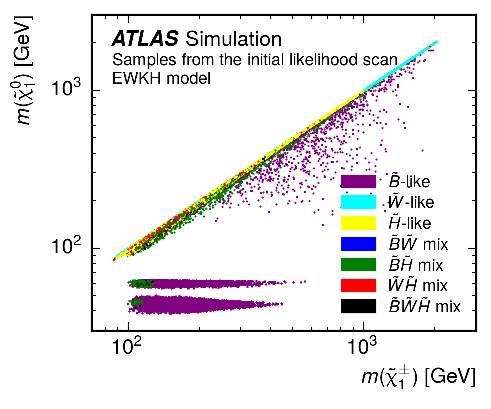
\includegraphics[scale=1.0]{LSP_composition.pdf}
        \caption{The scatter plot in the $m(\widetilde{\chi}^{0}_{1})$ vs $m(\widetilde{\chi}^{\pm}_{1})$ plane~\cite{Aaboud:2016wna}.
        The color encodes the $\widetilde{\chi}^{0}_{1}$ composition.
        The Higgsino-dominated LSPs are colored in yellow and along the $\widetilde{\chi}^{0}_{1}$-$\widetilde{\chi}^{\pm}_{1}$ diagonal.}
        \label{fig:intro_LSP_composition}
    \end{center}
\end{figure}

This dissertation focuses on searching for electroweak production of SUSY particles in compressed scenarios with exactly two low-momentum same-flavor opposite-charged leptons (electron and muon) in final states and missing transverse momentum $\textbf{p}_{\text{T}}^{\text{miss}}$.
This search uses proton-proton collision data at $\sqrt{s} = 13$~{\TeV} recorded by the ATLAS detector at the Large Hadron Collider (LHC)~\cite{Evans:2008zzb} in 2015 and 2016, corresponding to a total integrated luminosity of 36.1~\ifb.
Figure~\ref{fig:intro_feynman_diagrams} shows the Feynman diagrams representing the electroweakino productions with two leptons final state in association with an initial state radiated jet.
Same-flavor opposite-charged leptons come from the $\widetilde{\chi}^{0}_{2}$ decays in the $\widetilde{\chi}^{0}_{2} \widetilde{\chi}^{\pm}_{1}$ and $\widetilde{\chi}^{0}_{2} \widetilde{\chi}^{0}_{1}$ productions, and from the $\widetilde{\chi}^{\pm}_{1}$ decays in the $\widetilde{\chi}^{\pm}_{1} \widetilde{\chi}^{\mp}_{1}$ production.
The two leptons can be reconstructed in the detector and carry small transverse momentum  \pt.
However, the two LSPs are invisible and back-to-back in the rest frame of their parent electroweakinos.
Because they carry large momentum, the missing transverse energy \met is relatively large.
Similar searches have been performed using $\sqrt{s} = 8$~{\TeV} and $\sqrt{s} = 13$~{\TeV} by the ATLAS~\cite{Aad:2014vma, Aad:2014nua, Aad:2015eda, Aaboud:2016wna} and CMS~\cite{Khachatryan:2014qwa, Khachatryan:2015pot, Sirunyan:2017lae} experiments.
Combining with the results from the LEP experiments, the mass limits for sleptons and charginos are $m(\widetilde{e}_{R}) > 73$~{\GeV}, $m(\widetilde{\mu}_{R}) > 94.6$~{\GeV}, and $m(\widetilde{\chi}^{\pm}_{1}) > 103.5$~{\GeV} or 92.4~{\GeV} depending on the $\Delta m(\widetilde{\chi}^{0}_{1}, \widetilde{\chi}^{\pm}_{1})$.

\begin{figure}[htbp]
    \begin{center}
        \begin{subfigure}[b]{0.32\textwidth}
            \begin{center}
                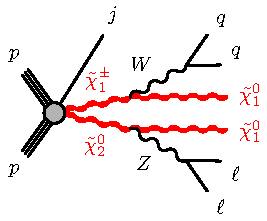
\includegraphics[scale=1.0]{C1N2-llqqN1N1g-WZ.pdf}
                \caption{The $\widetilde{\chi}^{0}_{2} \widetilde{\chi}^{\pm}_{1}$ production.}
            \end{center}
        \end{subfigure}%
        \begin{subfigure}[b]{0.32\textwidth}
            \begin{center}
                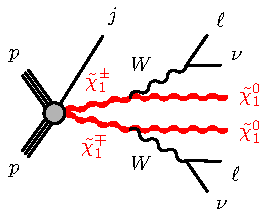
\includegraphics[scale=1.0]{C1C1-llvvN1N1g-WW.pdf}
                \caption{The $\widetilde{\chi}^{\pm}_{1} \widetilde{\chi}^{\mp}_{1}$ production.}
            \end{center}
        \end{subfigure}
        \begin{subfigure}[b]{0.32\textwidth}
            \begin{center}
                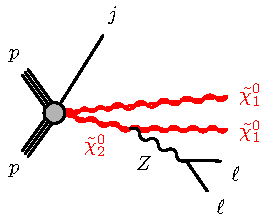
\includegraphics[scale=1.0]{N2N1-jllN1N1-Z.pdf}
                \caption{The $\widetilde{\chi}^{0}_{2} \widetilde{\chi}^{0}_{1}$ production.}
            \end{center}
        \end{subfigure}
    \end{center}
    \caption{The Feynman diagrams representing the two leptons final state of (a) $\widetilde{\chi}^{0}_{2} \widetilde{\chi}^{\pm}_{1}$, (b) $\widetilde{\chi}^{\pm}_{1} \widetilde{\chi}^{\mp}_{1}$, (c) $\widetilde{\chi}^{0}_{2} \widetilde{\chi}^{0}_{1}$ productions.}
    \label{fig:intro_feynman_diagrams}
\end{figure}

This dissertation has the following structure.
An introduction is given in Chapter~\ref{chapter:introduction} followed by theoretical foundations in Chapter~\ref{chapter:standard_model} and \ref{chapter:Supersymmetry}.
The experiment facilities are described in Chapter~\ref{chapter:altas_experiment}.
The data and Monte Carlo samples used are detailed in Chapter~\ref{chapter:data}.
Chapter~\ref{chapter:event_reconstruction_and_selection} presents the event reconstruction and the signal region selection.
The background estimation and the systematic uncertainties are discussed in Chapter~\ref{chapter:bkg_estimation}.
The results and interpretation are reported in Chapter~\ref{chapter:results}.
Finally, the conclusions are summarized in Chapter~\ref{chapter:conclusion}.



\chapter{The Standard Model}
\label{chapter:standard_model}
\graphicspath{{figures/standard_model/}}
This chapter outlines relevant theoretical and mathematical concepts of high energy particle physics.
The Standard Model of particle physics (SM)~\cite{Salam:1968rm, Glashow:1961tr, Weinberg:1967tq, Herrero:1998eq, Cottingham:2007zz} has been developed since the early 1970s and it has successfully explained almost all experimental results.
The SM is well-tested and the most successful physics theory to describe the nature of the elementary particles and their interactions.
An overview of the SM is given in Sect.~\ref{sec:sm}.
Then, some of the open questions are mentioned in Sect.~\ref{sec:sm_bsm}.

%%%
%%%
%%%

\section{The Standard Model of Particle Physics}
\label{sec:sm}
The Standard Model of particle physics is known as the most accurate theory for describing the elementary particles and the interactions between them.
By combining the quantum mechanics and special relativity, the SM is a relativistic \textit{Quantum Field Theory} (QFT) based on a $SU(3)_{C} \otimes SU(2)_{L} \otimes U(1)_{Y}$ symmetry gauge group, where $C$ denotes color, $L$ represents left chirality, and $Y$ stands for weak hypercharge, respectively.
The $SU(3)_{C}$ group is the basis for \textit{Quantum Chromodynamics} (QCD) which describes the strong interaction and the $SU(2)_{L} \otimes U(1)_{Y}$ group is the foundation of the electroweak interaction which unifies the electromagnetic and weak interactions.
Therefore, the SM Lagrangian is invariant under the local gauge transformation.
According to \textit{Noether's Theorem}~\cite{Noether:1918zz}, the invariance of an action of a physical system undergoes a symmetry transformation corresponding to a conservation law and vice versa. 
The gauge invariance of the SM Lagrangian corresponds to the conserved quantum numbers, or the charges, of each interaction.
The conserved charges are the three color charge (red, blue, green) for the strong interaction, the third component of the weak isospin $I_{3}$ for the weak interaction, and the electric charge $Q$ for the electromagnetic interaction.

%%%
%%%
%%%

\subsection{Particle Content}
\label{subsec:sm_particle_content}
According to the SM, all matter around us is made of elementary particles called \textit{quarks} and \textit{leptons}.
The quarks and leptons are called fermions which have half integral spin $s=\frac{1}{2}$, hence the fermions follow the Pauli exclusion principle which says no two fermions have the same quantum state at the same time.
Each fermion has an anti-fermion with the equal mass but carries opposite electric charge, weak isospin and color charge.
There are six quarks and six leptons, they are grouped into three pairs, or "\textit{generations}", ordered by their mass.
The lightest and most stable particles constitute the first generation and they are constituents of ordinary matter.
The heavier and less stable particles form the second and third generations and the heavier particles quickly decay to the next most stable particles.
The three generations of quarks are up ($u$) and down ($d$), charm ($c$) and strange ($s$), and top ($t$) and bottom ($b$) quarks.
The up-type quarks ($u, c, t$) carry $+\frac{2}{3}|e|$ charge and with isospin $+\frac{1}{2}$ while the down-type quarks ($d, s, b$) carry $-\frac{1}{3}|e|$ charge with isospin $-\frac{1}{2}$.
The quarks carry an additional color charge of either red, green, or blue, and hence they only interact via the strong force.
Because the strong force holds quarks together, only non-integer charges of the quark combinations are experimentally allowed.
The quark combinations are called \textit{hadrons} which can be categorized into \textit{mesons} and \textit{baryons}.
The meson is composed by a quark and anti-quark pair ($q\bar{q}$) whereas the baryon is made up by three quarks ($qqq$ or $\bar{q}\bar{q}\bar{q}$).
Only colorless bound states of hadrons are allowed so the quark and anti-quark pair in a meson should contain color and anti-color and the three quarks in a baryon must carry different colors.
The leptons are colorless and are therefore participating in the weak and electromagnetic force only. 
They do not participate in the strong interaction.
The electron-type leptons ($e, \mu, \tau$) carry an elementary charge $|e|$ and their corresponding neutrinos ($\nu_{e}, \nu_{\mu}, \nu_{\tau}$) are neutral.
The neutrinos have very little mass and interact via weak force only.
A summarized table of the properties of quarks and leptons is given in Table~\ref{tab:sm_fermions}.

\begin{table}[htp]
    %\begin{center}
    \resizebox{\textwidth}{!}{% <------ Don't forget this %
        \begin{tabular}{cccccccc}
            \hline
            \hline
            Generation           & Fermion                 &              & particle          & electric charge $Q$ & weak isospin $I_{3}$ & color charge $C$ & mass [{\GeV}]\\
            \hline
            \multirow{4}{*}{I}   & \multirow{2}{*}{Quark}  & $u$          & up quark          & $+\frac{2}{3}|e|$   & $+\frac{1}{2}$       & r,g,b             & 0.0023\\
                                 &                         & $d$          & down quark        & $-\frac{1}{3}|e|$   & $-\frac{1}{2}$       & r,g,b             & 0.0048\\
                                 & \multirow{2}{*}{Lepton} & $e$          & electron          & $-1|e|$             & $-\frac{1}{2}$       & -                 & 0.00051\\
                                 &                         & $\nu_{e}$    & electron neutrino & 0                   & $+\frac{1}{2}$       & -                 & $< 2 \times 10^{-9}$\\
            \hline
            \multirow{4}{*}{II}  & \multirow{2}{*}{Quark}  & $c$          & charm quark       & $+\frac{2}{3}|e|$   & $+\frac{1}{2}$       & r,g,b             & 1.275\\
                                 &                         & $s$          & strange quark     & $-\frac{1}{3}|e|$   & $-\frac{1}{2}$       & r,g,b             & 0.095\\
                                 & \multirow{2}{*}{Lepton} & $\mu$        & muon              & $-1|e|$             & $-\frac{1}{2}$       & -                 & 0.106\\
                                 &                         & $\nu_{\mu}$  & muon neutrino     & 0                   & $+\frac{1}{2}$       & -                 & $< 1.9 \times 10^{-7}$\\
            \hline
            \multirow{4}{*}{III} & \multirow{2}{*}{Quark}  & $t$          & top quark         & $+\frac{2}{3}|e|$   & $+\frac{1}{2}$       & r,g,b             & 173.2\\
                                 &                         & $b$          & bottom quark      & $-\frac{1}{3}|e|$   & $-\frac{1}{2}$       & r,g,b             & 4.18\\
                                 & \multirow{2}{*}{Lepton} & $\tau$       & tau               & $-1|e|$             & $-\frac{1}{2}$       & -                 & 1.777\\
                                 &                         & $\nu_{\tau}$ & tau neutrino      & 0                   & $+\frac{1}{2}$       & -                 & $< 1.82 \times 10^{-5}$\\
            \hline
            \hline
        \end{tabular}
    }
    %\end{center}
    \caption{The Standard Model fermions with charges and masses~\cite{Patrignani:2016xqp}.}
    \label{tab:sm_fermions}
\end{table}%

%\begin{figure}[htbp]
%   \begin{center}
%       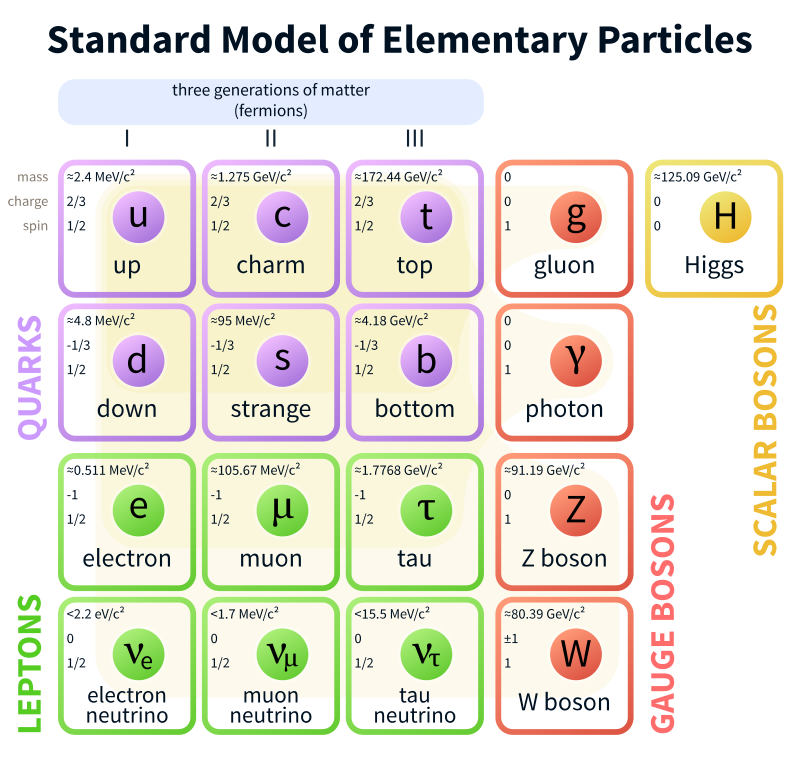
\includegraphics[scale=0.3]{800px-Standard_Model_of_Elementary_Particles.png}
%       \caption{default.
%       https://en.wikipedia.org/wiki/Standard_Model}
%       \label{fig:sm_particles}
%   \end{center}
%\end{figure}

There are four fundamental forces in the universe: the strong force, the weak force, the electromagnetic force, and the gravitational force.
The first three forces are described in the SM, however, the gravitational force could not yet be included in the SM.
Because the effect of the gravitational force is very weak and can be negligible, the SM works well without considering the gravitational force.
Each force has a force-carrier particle called gauge boson and there is a quantum number associate to it.
The gauge bosons of the strong force are eight massless \textit{gluons}, $g$, which associate to color charge $C$.
The gauge bosons of the weak force are $W^{\pm}$ and $Z^{0}$ bosons which associate to weak isospin $I_{3}$.
The gauge boson of the electromagnetic force is massless \textit{photon}, $\gamma$, which associates to electric charge $Q$.
Although the gluon and photon are massless particles, the $W^{\pm}$ and $Z^{0}$ bosons are massive.
The mass of the $W^{\pm}$ and $Z^{0}$ bosons are $m_{W}=80.385 \pm 0.015$~{\GeV} and $m_{Z}=91.1876 \pm 0.0021$~{\GeV}~\cite{Patrignani:2016xqp}, respectively.
Table~\ref{tab:sm_fundamental_forces} shows the four fundamental forces, the relative strength and range together with the theories and the mediators.

\begin{table}[htp]
    %\begin{center}
    \resizebox{\textwidth}{!}{% <------ Don't forget this %
        \begin{tabular}{cccccc}
            \hline
            \hline
            Force           & Rel. Strength & Range [m]  & Theory             & Mediator                     & Mass [{\GeV}]\\
            \hline
            Strong          & $10$          & $10^{-15}$ & Chromodynamics     & Gluon                        & 0\\
            Weak            & $10^{-13}$    & $10^{-18}$ & Flavourdynamics    & $W^{\pm}$ and $Z^{0}$ bosons & 80.4/91.2\\
            Electromagnetic & $10^{-2}$     & $\infty$   & Electrodynamics    & Photon                       & 0\\
            \hline
            Gravitational   & $10^{-42}$    & $\infty$   & General relativity & Graviton                     & -\\
            \hline
            \hline
        \end{tabular}
    }
    %\end{center}
    \caption{The four fundamental forces with the relative strength, interaction range, describing theory, and the mediator with its mass.
    The gravitational force is not a part of the SM and the graviton is a theoretical particle.}
    \label{tab:sm_fundamental_forces}
\end{table}%

%%%
%%%
%%%

\subsection{Local Gauge Theory}
\label{subsec:sm_gauge_theory}
The Lagrangian density of the SM for the free fields\footnote{This is the Lagrangian density of QED. The three terms are fermion kinematic term, photon kinematic term, and interaction, respectively.} listed in the Eq.~(\ref{eq:sm_lagrangian}) is invariant under local gauge transformation\footnote{In Dirac representation, the four contravariant gamma matrices are $\gamma^{0} = \left(\begin{matrix}1 & 0 & 0 & 0\\0 & 1 & 0 & 0\\0 & 0 & -1 & 0\\0 & 0 & 0 & -1\end{matrix}\right)$, $\gamma^{1} = \left(\begin{matrix}0 & 0 & 0 & 1\\0 & 0 & 1 & 0\\0 & -1 & 0 & 0\\-1 & 0 & 0 & 0\end{matrix}\right)$, $\gamma^{2} = \left(\begin{matrix}0 & 0 & 0 & -i\\0 & 0 & i & 0\\0 & i & 0 & 0\\-i & 0 & 0 & 0\end{matrix}\right)$, $\gamma^{3} = \left(\begin{matrix}0 & 0 & 1 & 0\\0 & 0 & 0 & -1\\-1 & 0 & 0 & 0\\0 & 1 & 0 & 0\end{matrix}\right)$}
%
\begin{equation}
    \mathcal{L} = \bar{\psi}(i\gamma^{\mu}\partial_{\mu} - m)\psi + e\bar{\psi}\gamma^{\mu}\psi\bm{A}_{\mu} - \frac{1}{4}\bm{F}_{\mu\nu}\bm{F}^{\mu\nu}
    \label{eq:sm_lagrangian}
\end{equation}
%
where $\bm{F}_{\mu\nu} = \partial_{\mu}\bm{A}_{\nu} - \partial_{\nu}\bm{A}_{\mu}$.
The local gauge transformation means the scalar field $\psi$ and the vector field $\bm{A}_{\mu}$ transform as
%
\begin{align}
    \psi(x) & \rightarrow \psi'(x) = e^{i\theta(x)}\psi(x)\\
    \bm{A}_{\mu}(x) & \rightarrow \bm{A}_{\mu}'(x) = \bm{A}_{\mu}(x) + \frac{1}{e}\partial_{\mu}\theta(x).
    \label{eq:sm_gauge_transformation}
\end{align}
%
By introducing the gauge term, i.e. the vector field, the interacting force can be obtained by calculating the derivatives of the \textit{Euler-Lagrange equations}.
The gauge field can be associated to particular spin one gauge bosons which mediate the force.
The number of the mediating gauge bosons is equal to the dimension of the symmetry group.
From the group theory, the dimension of an unitary group $U(n)$ is $n^{2}$ and the dimension of a special unitary group $SU(n)$ is $n^{2} - 1$.
Because the SM is based on a $SU(3)_{C} \otimes SU(2)_{L} \otimes U(1)_{Y}$ symmetry gauge group, the number of mediators are 8 for $SU(3)_{C}$, 3 for $SU(2)_{L}$, and 1 for $U(1)_{Y}$ corresponding to 8 gluons for the strong interaction, 3 gauge bosons ($W^{\pm}$ and $Z^{0}$) for weak interaction, and 1 photon for the electromagnetic interaction.


%%%
%%%
%%%

\subsection{Strong interaction}
\label{subsec:sm_strong_interaction}
The \textit{Quantum Chromodynamics} (QCD) is the theory to describe the strong interaction.
The gauge bosons are the eight massless gluons which carry three different colors (and anti-colors), red, green, and blue.
Quarks interact with gluons hence they also carry color charge $C$ and can be represented in color triplets
%
\begin{equation}
    \psi = 
    \left(
        \begin{matrix}
            & \psi_{r} & \\
            & \psi_{g} & \\
            & \psi_{b} &
        \end{matrix}
    \right).
    \label{eq:sm_quark_triplets}
\end{equation}
%
The QCD is based on the non-Abelian $SU(3)_{C}$ group which requires local gauge transformation
%
\begin{equation}
    \psi \rightarrow \psi' = e^{i g_{s} \alpha_{a}(x) T^{a}}\psi
    \label{eq:sm_qcd_gauge_transformation_1}
\end{equation}
%
where the $g_{s}$ is the strong coupling constant, $\alpha_{a}(x)$ are arbitrary functions of space-time, and $T^{a}$ are the generators of the non-Abelian $SU(3)_{C}$ group and the summation over $a$ with $a = 1, \dots, 8$ is implied.
The Lagrangian density is invariant under the local gauge transformation by introducing the new form of the gauge fields and the covariant derivative
%
\begin{align}
    \bm{G}_{\mu}^{a} & \rightarrow \bm{G}_{\mu}^{a} -  \partial_{\mu} \alpha^{a}(x) - g_{s} f_{abc} \alpha^{b}(x) \bm{G}_{\mu}^{c} \\
    \partial_{\mu} & \rightarrow D_{\mu} = \partial_{\mu} + i g_{s} T_{a} \bm{G}_{\mu}^{a}
    \label{eq:sm_qcd_gauge_transformation_2}
\end{align}
%
where $f_{abc}$ is the structure constant. 
The Lagrangian density of QCD is given by
%
\begin{equation}
    \mathcal{L}_{QCD} = \bar{\psi}(i \gamma^{\mu} \partial_{\mu} - m) \psi - g_{s} ( \bar{\psi} \gamma^{\mu} T_{a} \psi) \bm{G}_{\mu}^{a} - \frac{1}{4} \bm{G}_{\mu\nu}^{a} \bm{G}_{a}^{\mu\nu}
    \label{eq:sm_qcd_lagrangian}
\end{equation}
%
where the field strength tensor $\bm{G}_{\mu\nu}^{a} = \partial_{\mu} \bm{G}_{\nu}^{a} - \partial_{\nu} \bm{G}_{\mu}^{a} - g_{s} f_{abc} \bm{G}_{\mu}^{b} \bm{G}_{\nu}^{c}$ causing self-interactions between the gluons.
The strong force increases with distance between quarks, therefore, the quarks exist only as colorless compounds such as meson or baryon mentioned in Sect.~\ref{subsec:sm_particle_content}.
The production of a single quark is accompanied by the creation of an anti-quark from vacuum to form a quark and anti-quark pair as a colorless compound.
This is called \textit{hadronisation}.
The phenomena that confined quarks in the small interaction range is called \textit{confinement}.
But at small distance or high energy, the quarks can be considered as quasi-free particles.
This is referred to as \textit{asymptotic freedom}.

%%%
%%%
%%%

\subsection{Electroweak interaction}
\label{subsec:sm_ewk_interaction}
Fermi formulated the first weak interaction theory in 1933~\cite{Fermi:1934hr}, however, the theory only holds for energies less than 100~{\GeV}.
Glashow, Salam, and Weinberg (GSW) proposed a new model~\cite{Salam:1968rm, Weinberg:1967tq, Glashow:1961tr} which unifies electromagnetic and weak forces to become \textit{electroweak} (EW) force and this new \textit{GSW model} can apply to the energy greater than 100~{\GeV}.
The electroweak theory is based on $SU(2)_{L} \otimes U(1)_{Y}$ gauge symmetry where the subscripts $L$ denotes the left-handedness because only the left-handed fermions (and right-handed anti-fermions) and $Y$ denotes the weak hypercharge, a new quantum number, which relates to the electric charge $Q$ and the weak isospin $I_{3}$ by the \textit{Gell-Mann-Nishijima relation}~\cite{Nakano:1953zz, Gell-Mann:1956iqa}
%
\begin{equation}
    Y = 2(Q - I_{3}).
    \label{eq:sm_hypercharge}
\end{equation}
%
The left-handed and right-handed fermion field $\psi$ can be decomposed into two components
%
\begin{align}
    \psi & = P_{L}\psi + P_{R}\psi\\
         & = \psi_{L} + \psi_{R}
    \label{eq:sm_fermion_field_components}
\end{align}
%
where the projection operators $P_{L}$ and $P_{R}$ are defined as\footnote{$\gamma^{5}$ is the product of the four gamma matrices. $\gamma^{5} = i \gamma^{0} \gamma^{1} \gamma^{2} \gamma^{3} = \left(\begin{matrix}0 & 0 & 1 & 0\\0 & 0 & 0 & 1\\1 & 0 & 0 & 0\\0 & 1 & 0 & 0\end{matrix}\right)$}
%
\begin{align}
    P_{L} & = \frac{1}{2} (1 - \gamma^{5})\\
    P_{R} & = \frac{1}{2} (1 + \gamma^{5}).
    \label{eq:sm_projection_operators}
\end{align}
%
The projection operators satisfy $P_{L}P_{R} = 0$ and $P_{L} + P_{R} = 1$.
Experimental observations show the right-handed neutrinos don't participate in all the interactions described in the SM so the $\psi_{R}$ is a singlet and $I_{3} = 0$\footnote{The left-handed fermion state $\psi_{L}$ is a doublet.}.
The local gauge transformations of the $SU(2)_{L} \otimes U(1)_{Y}$ are
%
\begin{align}
    \psi_{L} & \rightarrow \psi_{L}' = e^{i \alpha_{a}(x) T^{a}}e^{i \beta(x) Y} \psi_{L}\\
    \psi_{R} & \rightarrow \psi_{R}' = e^{i \beta(x) Y} \psi_{R}
    \label{eq:sm_local_gauge_transformations_ew_1}
\end{align}
%
where $T^{a} = \frac{\sigma^{a}}{2}$ are the generators of $SU(2)_{L}$ with Pauli matrix $\sigma^{a}$\footnote{The Pauli matrices are $\sigma_{1}=\left(\begin{matrix}0 & 1\\1 & 0\end{matrix}\right)$, $\sigma_{2}=\left(\begin{matrix}0 & -i\\i & 0\end{matrix}\right)$, and $\sigma_{3}=\left(\begin{matrix}1 & 0\\0 & -1\end{matrix}\right)$} and $Y$ is the generator of $U(1)_{Y}$.
The $\alpha_{a}(x)$ and $\beta(x)$ depend on the space-time.
The covariant derivative with respect to the $SU(2)_{L} \otimes U(1)_{Y}$ is
%
\begin{equation}
    D_{\mu} = \partial_{\mu} + i g_{W} T_{a} \bm{W}_{\mu}^{a} + i g_{Y} Y \bm{B}_{\mu}
    \label{eq:sm_derivative_ew}
\end{equation}
%
where $g_{W}$ and $g_{Y}$ are coupling constants and $\bm{W}_{\mu}^{a}$ ($a = 1, 2, 3$) and $\bm{B}_{\mu}$ are the gauge fields.
The gauge fields $\bm{W}_{\mu}^{a}$ and $\bm{B}_{\mu}$ transform under the $SU(2)_{L} \otimes U(1)_{Y}$ symmetry as
%
\begin{align}
    \bm{W}_{\mu}^{a} & \rightarrow \bm{W}_{\mu}^{a} - \frac{1}{g_{W}} \partial_{\mu} \alpha^{a}(x) - \epsilon^{abc} \alpha^{b}(x) \bm{W}_{\mu}^{c}\\
    \bm{B}_{\mu} & \rightarrow \bm{B}_{\mu} - \frac{1}{g_{Y}} \partial_{\mu} \beta(x)
    \label{eq:sm_local_gauge_transformations_ew_2}
\end{align}
%
where $\epsilon^{abc}$ is the Levi-Civita tensor.
The Lagrangian density of the electroweak is given by
%
\begin{equation}
    \mathcal{L}_{EW} = \bar{\psi}_{L} (i \gamma^{\mu} D_{\mu} - m) \psi_{L} + \bar{\psi}_{R} (i \gamma^{\mu} D_{\mu} - m) \psi_{R} - \frac{1}{4} \bm{W}_{\mu\nu}^{a} \bm{W}_{a}^{\mu\nu} - \frac{1}{4} \bm{B}_{\mu\nu} \bm{B}^{\mu\nu}
    \label{eq:sm_Lagrangian_ew}
\end{equation}
%
where $\bm{W}_{\mu\nu}^{a}$ and $\bm{B}_{\mu\nu}$ are the field strength tensors
%
\begin{align}
    \bm{W}_{\mu\nu}^{a} & = \partial_{\mu} \bm{W}_{\nu}^{a} - \partial_{\nu} \bm{W}_{\mu}^{a} - g_{W} \epsilon^{abc} \bm{W}_{\mu}^{b} \bm{W}_{\nu}^{c}\\
    \bm{B}_{\mu\nu} & = \partial_{\mu} \bm{B}_{\nu} - \partial_{\nu} \bm{B}_{\mu}
    \label{eq:sm_field_strangth_tensors}
\end{align}
%
and $\bar{\psi} \equiv \psi^{\dagger} \gamma^{0}$ is the adjoint spinor of $\psi$\footnote{$\psi^{\dagger}$ is the hermitian conjugate of $\psi$}.
Therefore, the mass eigenstates are the mixture of the gauge fields
%
\begin{align}
    \bm{W}_{\mu}^{\pm} & = \frac{1}{\sqrt{2}} (\bm{W}_{\mu}^{1} \mp i \bm{W}_{\mu}^{2})\\
    \left(\begin{matrix}\bm{A}_{\mu}\\\bm{Z}_{\mu}\end{matrix}\right) & = \left(\begin{matrix}\cos\theta_{W} & \sin\theta_{W}\\-\sin\theta_{W} & \cos\theta_{W} \end{matrix}\right) \left(\begin{matrix}\bm{B}_{\mu}\\\bm{W}_{\mu}^{3}\end{matrix}\right).
    \label{eq:sm_mass_eigenstates}
\end{align}
%
Thus, the mass eigenstates $\bm{A}_{\mu}$, $\bm{W}_{\mu}^{\pm}$, and $\bm{Z}_{\mu}$ are identified as the photon, $\gamma$, $W^{\pm}$ and $Z^{0}$ bosons experimentally.
The \textit{Weinberg weak mixing angle} $\theta_{W}$ is defined as
%
\begin{equation}
    \tan \theta_{W} = \frac{g_{Y}}{g_{W}}.
    \label{eq:sm_mixing_angle}
\end{equation}
%
The coupling constants $g_{W}$ and $g_{Y}$ are related to the electric charge by
%
\begin{equation}
    e = g_{W} \sin\theta_{W} = g_{Y} \cos\theta_{Y}.
    \label{eq:sm_coupling_constants}
\end{equation}
%
And the weak eigenstates of quark, $q'$, are the linear combinations of the mass eigenstates of quark, q, by the \textit{Cabbibo-Kobayashi-Maskawa} (CKM) matrix~\cite{Kobayashi:1973fv}
%
\begin{equation}
    \left(\begin{matrix}d'\\s'\\b'\end{matrix}\right) = \left(\begin{matrix}V_{ud} & V_{us} & V_{ub}\\V_{cd} & V_{cs} & V_{cb}\\V_{td} & V_{ts} &V_{tb}\end{matrix}\right) \left(\begin{matrix}d\\s\\b\end{matrix}\right).
    \label{eq:sm_CKM_matrix}
\end{equation}
%
The CKM matrix allows the quarks changing their flavor and generation as observed in the experiment.
Similarly, the \textit{Pontecorvo-Maki-Nakagawa-Sakata} (PMNS) matrix~\cite{Maki:1962mu} is responsible for the flavor changing of the neutrinos.

%%%
%%%
%%%

\subsubsection{Spontaneous symmetry breaking and Higgs mechanism}
\label{subsubsec:sm_Higgs_mechanism}
The gauge bosons of the weak interaction, $W^{\pm}$ and $Z^{0}$, are massive particles\footnote{$m_{W}=80.385 \pm 0.015$~{\GeV} and $m_{Z}=91.1876 \pm 0.0021$~{\GeV}}.
However, the existence of the mass terms violate the gauge invariance of the $\mathcal{L}_{EW}$.
In order to explain the mass of gauge bosons, the Englert-Brout-Higgs mechanism~\cite{Higgs:1966ev, Higgs:1964pj, Higgs:1964ia, Englert:1964et, Guralnik:1964eu} was proposed in 1964.
A new scalar complex $SU(2)_{L}$ doublet field $\Phi$ is introduced in the Higgs mechanism
%
\begin{equation}
    \Phi = \left(\begin{matrix}\Phi^{+}\\\Phi^{0}\end{matrix}\right) = \left(\begin{matrix}\Phi_{1} & i\Phi_{2}\\\Phi_{3} & i\Phi_{4}\end{matrix}\right)
    \label{eq:sm_higgs_doublet}
\end{equation}
%
with hypercharge $Y = 1$ and four degrees of freedom, $\Phi_{i}$, which are scalar fields and called the \textit{Goldstone modes}.
The Lagrangian density for this new field, Higgs field, is
%
\begin{equation}
    \mathcal{L}_{\Phi} = (D^{\mu}\Phi)^{\dagger}(D_{\mu}\Phi) - V(\Phi)
    \label{eq:sm_higgs_lagrangian}
\end{equation}
%
where the Higgs potential is defined as
%
\begin{equation}
    V(\Phi) = \mu^{2}|\Phi|^{2} + \lambda|\Phi|^{4}
    \label{eq:sm_higgs_potential}
\end{equation}
%
where $\mu$ and $\lambda$ are free parameters.
The Higgs potential is shown in Fig.~\ref{fig:sm_higgs_potential}.
The Higgs potential is the rotation $U(1)$ symmetry.
Choosing any of the points at the bottom of the Higgs potential breaks the symmetry spontaneously.
The \textit{spontaneously symmetry breaking} (SSB) means the Lagrangian keeps invariant under certain symmetry but no longer invariant at the ground state.

\begin{figure}[htbp]
    \begin{center}
        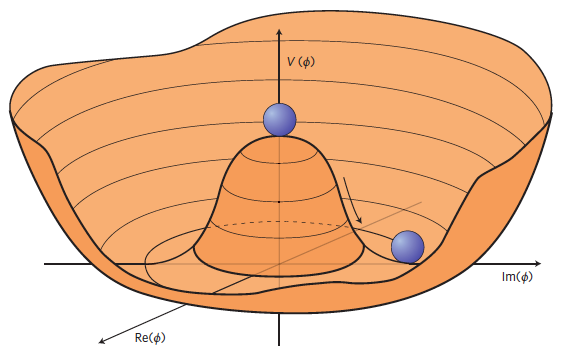
\includegraphics[scale=0.4]{higgspotential.png}
        \caption{An illustration of the Higgs potential which has the form of a ``Mexican hat''~\cite{Ellis:2013jnq}.}
        \label{fig:sm_higgs_potential}
    \end{center}
\end{figure}

Because the Higgs potential is invariant under $SU(2)_{L} \otimes U(1)_{Y}$, the parameters $\mu$ and $\lambda$ must satisfy $\mu^{2} < 0$ and $\lambda > 0$ resulting in a set of degenerate ground states where $\langle 0|\Phi|0 \rangle \neq 0$.
Among the degenerate ground states, the ground state is often chosen to have the form
%
\begin{equation}
    \Phi = \frac{1}{\sqrt{2}}\left(\begin{matrix}0\\v\end{matrix}\right)
    \label{eq:sm_ground_state}
\end{equation}
%
where $v = \sqrt{-\mu^{2}/\lambda}$ is the \textit{the vacuum expectation value} (VEV).
This particular choice of the ground state breaks the $SU(2)_{L} \otimes U(1)_{Y}$ symmetries spontaneously and  ensures the unbroken electromagnetic interaction under $U(1)_{EM}$ symmetry and photon being massless.
By introducing a massive particle, Higgs boson $H$, the Higgs field can be re-written as
%
\begin{equation}
    \Phi = \frac{1}{\sqrt{2}}\left(\begin{matrix}0\\v + H\end{matrix}\right)
    \label{eq:sm_ground_state_2}
\end{equation}
%
and the kinematic term of the Lagrangian density becomes
%
\begin{align}
    \mathcal{L}_{\Phi}^{\textrm{kinematic}} & = (D^{\mu}\Phi)^{\dagger}(D_{\mu}\Phi)\\
                                            & = \frac{1}{2}\partial_{\mu}H\partial^{\mu}H + (v + H)^{2}\Big\{\frac{g_{W}^{2}}{4} \bm{W}_{\mu}^{\dagger}\bm{W}^{\mu} + \frac{g_{W}^{2}}{8\cos^{2}\theta_{W}}\bm{Z}_{\mu}^{\dagger}\bm{Z}^{\mu}\Big\}
    \label{eq:sm_Lagrangian_kinematic_term}
\end{align}
%
and the Higgs potential is now
%
\begin{equation}
    V(\Phi) = -\frac{v^{2} \lambda}{2}(v+H)^{2} + \frac{\lambda}{4}(v+H)^{4}.
\end{equation}
%
Thus the masses of the $W^{\pm}$ and $Z^{0}$ are obtained by the interaction between the gauge bosons and Higgs boson.
The masses are defined as
%
\begin{equation}
    m_{H} = v\sqrt{2\lambda}, \quad m_{W} = \frac{v}{2}g_{W}, \quad m_{Z} = \frac{v}{2}\sqrt{g_{W}^{2} + g_{Y}^{2}}, \quad m_{\gamma} = 0.
\end{equation}
%
However, the masses of fermions are obtained by the \textit{Yukawa interaction}
%
\begin{equation}
    \mathcal{L}_{\textrm{Yukawa}} = y_{f} \bar{L}_{L} \Phi f_{R} + y_{f} \bar{Q}_{L} \Phi f_{R} + \textrm{h.c.}
\end{equation}
%
where the $y_{f}$ is \textit{Yukawa coupling}, $f$ stands for \{$\ell^{i}$, $u^{i}$, $d'^{i}$\} and h.c. represents the hermitian conjugate, respectively.
The $\bar{L}_{L}$ and $\bar{Q}_{L}$ are the left-handed lepton and quark doublet and $f_{R}$ is the lepton or quark singlet.
The mass of fermion is defined as
%
\begin{equation}
    m_{f} = \frac{v}{\sqrt{2}}y_{f}
\end{equation}
%
where $y_{f}$ is a free parameter which causes the fermion mass not predictable.
Finally, the non-zero VEV, $v$, can be related to \textit{Fermi constant}, $G_{F}$, by
%
\begin{equation}
    v = \frac{1}{\sqrt{\sqrt{2} G_{F}}} \approx 246 \textrm{~{GeV}}.
\end{equation}
%

%%%
%%%
%%%

\subsection{The discovery of Higgs boson}
A lot of the SM predictions are successfully confirmed by the experimental observations besides the existence of the theoretical Higgs boson. 
The search of the Higgs boson has become a major goal of the experimental particle physicists.
A Higgs-like resonance was discovered and announced on July 4th 2012 by the ATLAS\footnote{A Toroidal LHC ApparatuS} and CMS\footnote{Compact Muon Solenoid} collaborations~\cite{Aad:2012tfa, Chatrchyan:2012xdj}.
By combining the data with integrated luminosities of 4.8~{\ifb} collected at $\sqrt{s} = 7$~{\TeV} in 2011 and 5.8~{\ifb} at $\sqrt{s}=8$~{\TeV} in 2012, the ATLAS experiment measured the mass of the Higgs boson to be $126.0 \pm 0.4$ (stat.) $\pm 0.4$ (syst.)~{\GeV} with significance of 5.9$\sigma$ corresponding to a background fluctuation probability of $1.7 \times 10^{-9}$~\cite{Aad:2012tfa}.
In the meantime, the CMS experiment announced the mass of the Higgs boson to be $125.3 \pm 0.4$ (stat) $\pm 0.5$ (syst.)~{\GeV} with significance 5.0$\sigma$ using integrated luminosities of up to 5.1~{\ifb} at 7 TeV and 5.3~{\ifb} at 8 TeV~\cite{Chatrchyan:2012xdj}. 
The $H \rightarrow ZZ^{(*)} \rightarrow 4\ell$, $H \rightarrow \gamma \gamma$, and $H \rightarrow WW^{(*)} \rightarrow e\nu\mu\nu$ channels were studied by the ATLAS collaboration and the $H \rightarrow \gamma \gamma, ZZ, W^{+}W^{-}, \tau^{+}\tau^{-}$, and $b\bar{b}$ channels were studied by the CMS collaboration.
In the Fig.~\ref{fig:sm_discovery_of_Higgs} shows the local $p$-value as a function of the Higgs mass for ATLAS and CMS results, respectively.

\begin{figure}[htbp]
    \begin{center}
        \begin{subfigure}[b]{0.48\textwidth}
            \begin{center}
                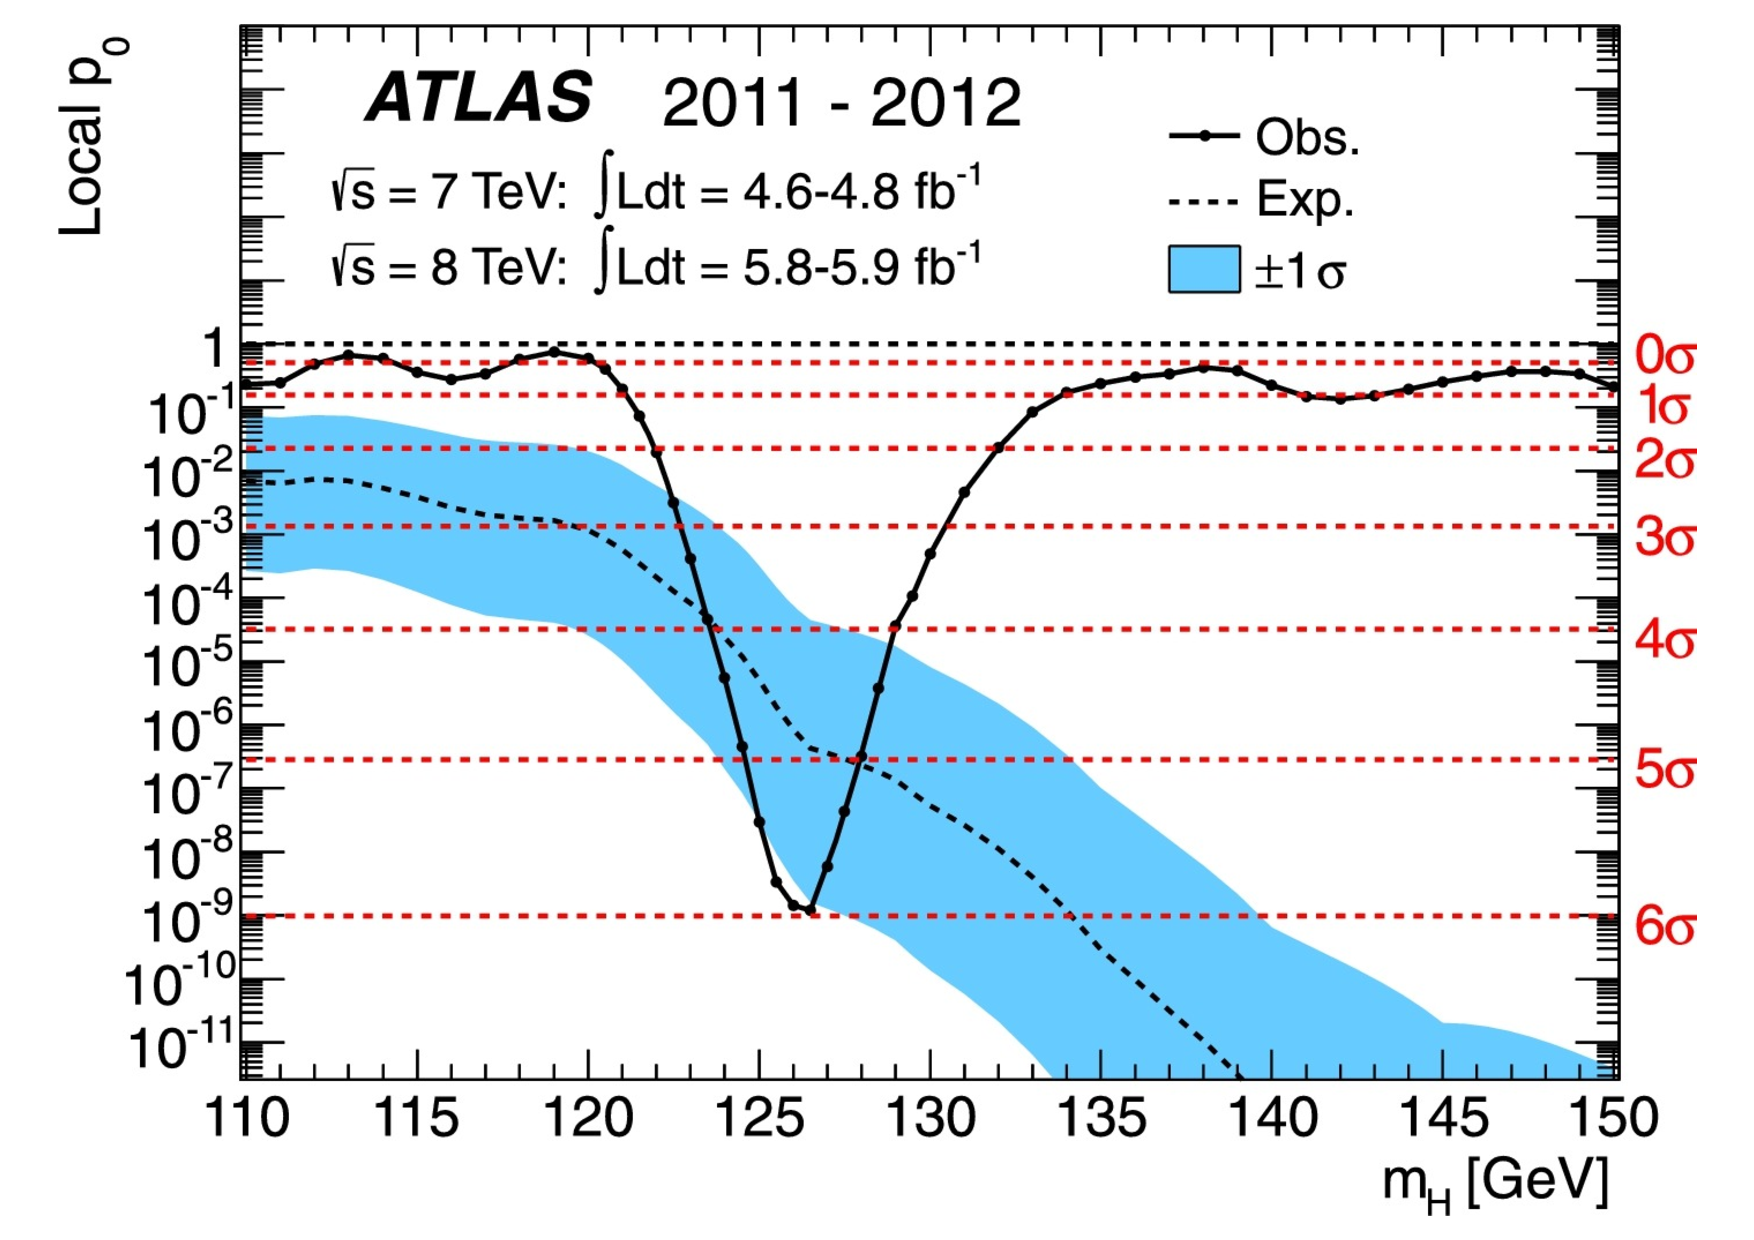
\includegraphics[scale=0.23]{1-s2_0-S037026931200857X-gr009_lrg.pdf}
                \caption{ATLAS results}
            \end{center}
        \end{subfigure}%
        \begin{subfigure}[b]{0.48\textwidth}
            \begin{center}
                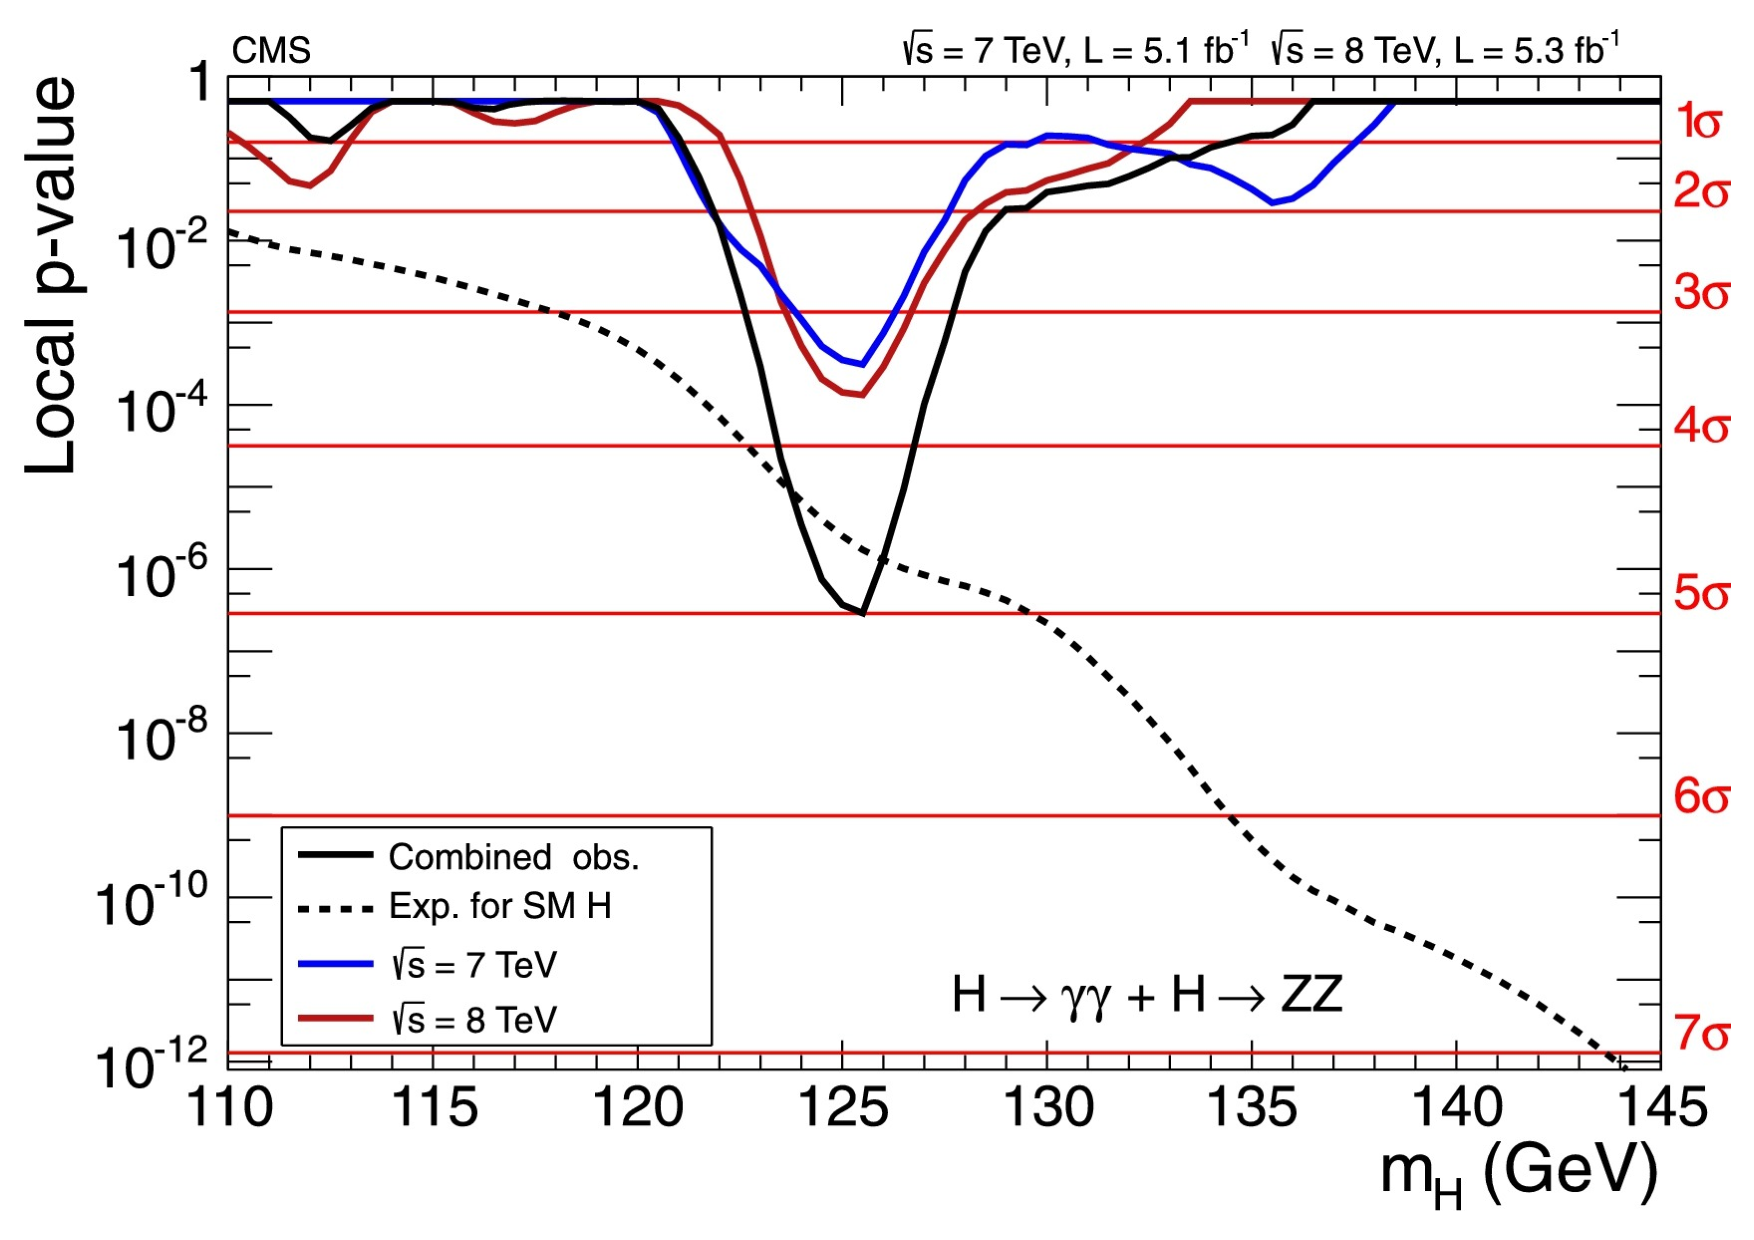
\includegraphics[scale=0.23]{1-s2_0-S0370269312008581-gr016_lrg.pdf}
                \caption{CMS results}
            \end{center}
        \end{subfigure}
    \end{center}
    \caption{The observed local $p$-value as a function of \mH for the ATLAS~\cite{Aad:2012tfa} and CMS~\cite{Chatrchyan:2012xdj} experiment, respectively.
    The dashed line shows the expected local $p_{0}$ for a SM Higgs boson.
    The horizontal lines denotes the $p$-values corresponding to significances of 1 to 6$\sigma$.}
    \label{fig:sm_discovery_of_Higgs}
\end{figure}

%%%
%%%
%%%

\section{Beyond the Standard Model}
\label{sec:sm_bsm}
Although the SM is an incredible successful theory for explaining the phenomenon in the particle physics, it leaves some questions which can no be answered.
Some of the unanswered questions are introduced in the rest part of this section.

%%%
%%%
%%%

\subsection{Hierarchy problem}
\label{subsec:sm_hierarchy_problem}
The weakest force in the SM is the weak force but the strength of the weak force is $10^{24}$ times as strong as gravitational force which doesn't incorporate into the SM.
The large discrepancy between the weak force and the gravitational force is called the hierarchy problem~\cite{Martin:1997ns, Chankowski:1998za, maarten_brak}.
The classical potential of the SM Higgs field $\Phi$ is
%
\begin{equation}
    V(\Phi) = \mu^{2} |\Phi|^2 + \lambda |\Phi|^4.
\end{equation}
%
Since the SM requires the VEV for $\Phi$, $\langle \Phi \rangle$, at the minimum of the potential non-vanishing, this only satisfied if $\mu^{2} < 0$ and $\lambda > 0$.
However, the parameter $\mu^{2}$ receives enormous radiative corrections causing it ultraviolet divergent as shown in Eq.~(\ref{eq:sm_mu2_correction}).
%
\begin{equation}
    \mu^{2} = \mu_{bare}^{2} - \frac{|\lambda_{f}|^{2}}{8\pi}\Lambda_{UV}^{2} + \mathcal{O}(\Lambda_{UV}^{2})
    \label{eq:sm_mu2_correction}
\end{equation}
%
where $\mu_{bare}$ is the Higgs mass, $- \frac{|\lambda_{f}|^{2}}{8\pi}\Lambda_{UV}^{2}$ is the one-loop correction, and $\Lambda_{UV}$ is an ultraviolet momentum cutoff which is valid up to the Plank scale $10^{19}$~{\GeV}.
The electroweak gauge bosons $W^{\pm}$ and $Z^{0}$ obtain their finite masses from $\langle \Phi \rangle$ so the $\mu^{2}$ cannot be divergent.
There must some unknown mechanism to protect from divergence.

%%%
%%%
%%%

\subsection{Dark matter and dark energy}
\label{subsec:sm_dm}
The matters we know today compose of only 5\%~\cite{Bennett:2012zja, Ade:2013sjv} of the content of the universe and the remaining part is something we don't know.
This unknown matter is called \textit{Dark Matter} (DM)~\cite{Bertone:2004pz} which makes up about 27\% of the universe and the rest 68\% are called \textit{Dark Energy} (DE)~\cite{Bennett:2012zja, Ade:2013sjv}.
Because DM interacts weakly and doesn't interact with the electromagnetic force, it doesn't absorb, emit, or reflect light causing it hard to detect directly. 
The name DM comes from it is invisible.
Dark energy distributes evenly in both space and time throughout the universe so it doesn't dilute when the universe expands.
The observed scientific data hints the presence of DE is necessary to explain the accelerated expansion of the universe.

%%%
%%%
%%%

\subsection{Grand Unification}
\label{subsec:sm_grand_unification}

\begin{figure}[tbp]
    \begin{center}
        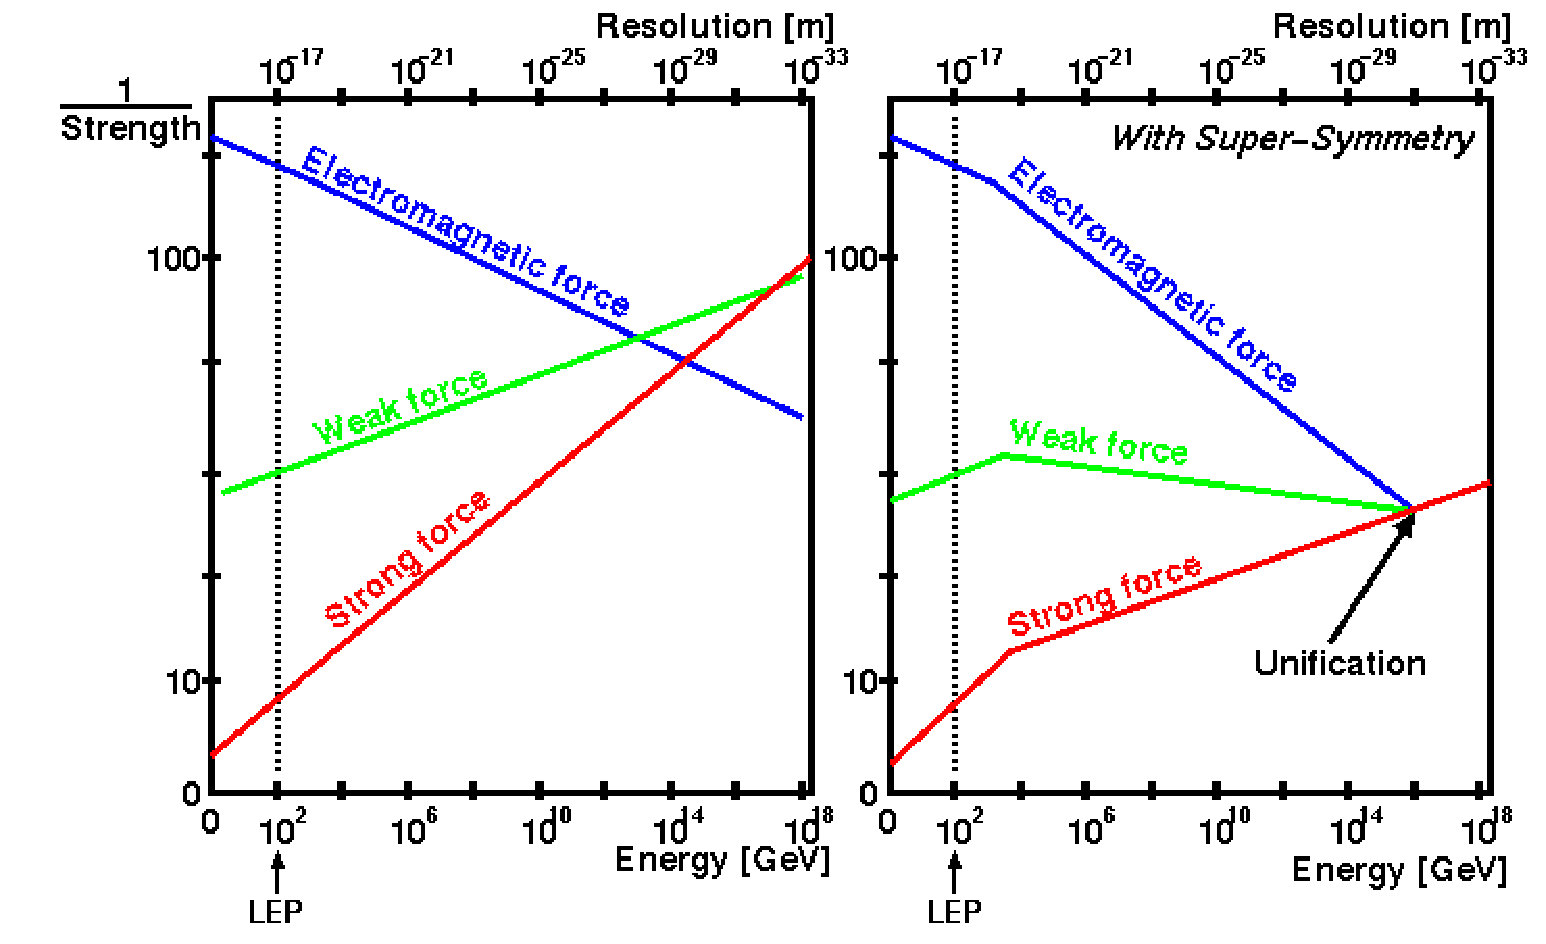
\includegraphics[scale=0.46]{running_coupling.pdf}
        \caption{The measured running coupling constants in the SM (left) and prediction in the GUT (right)~\cite{Ur0ol}.
        The three lines show the inverse value of the coupling constant for the three fundamental forces.}
        \label{fig:sm_coulping_constants}
    \end{center}
\end{figure}

Maxwell unified the electricity and magnetism into electromagnetism in the 1860s.
About a century later, physicists successfully developed theory of electroweak which links the electromagnetism and the weak force.
Because of the triumph of electroweak theory, theorists raise the question of the possibility to unify all forces.
The \textit{Grand Unified Theory} (GUT)~\cite{Ross:1985ai}, which tries to link three of the four known forces together, is developed in the mid-1970s by theorists
The GUT proposes that the electromagnetic force, weak force, and strong force unify to one force at the GUT scale, $\Lambda_{GUT} \approx 10^{16}$~{\GeV}.
So the three running coupling constants~\cite{Mohr:2015ccw} are expected to be converged at the GUT scale.
However, the current experiment results show the coupling constants still different as shown in Fig.~\ref{fig:sm_coulping_constants}.

%%%
%%%
%%%

\subsection{More questions}
\label{subsec:sm_more_questions}
There are some more interesting questions which we don't know the answers.
For example, we don't know the reason why there are 61 elementary particles and more than 20 arbitrary parameters in the SM.
Also, the SM doesn't explain why there are only three generations.
The amount of matter and anti-matter are equal at the beginning of the universe based on the prediction of the SM but the matter dominates in the currently universe which the SM couldn't answer the reason why.

In order to answer these questions, there are many theories being developed on the top of SM but none of them has been observed.
One of the most probable candidate for answering these question is supersymmetry which will be introduced in the next chapter.



\chapter{Suppersymmetry}
\label{chapter:Suppersymmetry}
\graphicspath{{figures/susy/}}
The SM~\cite{Salam:1968rm, Glashow:1961tr, Weinberg:1967tq, Herrero:1998eq, Cottingham:2007zz} gets a stupendous success in expecting and explaining the physics phenomena of the elementary particles.
However, the SM leaves several open questions unanswered as mentioned in Sect.~\ref{sec:sm_bsm}.
Many different models of new physics were proposed to explain those unanswered questions.
Among these new models, the \textit{supersymmetry} (SUSY)~\cite{Wess:1974tw, Lykken:1996xt, Drees:1996ca, Martin:1997ns, Bilal:2001nv, Argyres:2001eva, Peskin:2008nw, Aitchison:2005cf, Shadmi:2017qdk} wins most physicists' favour.
The SUSY proposed by Wess and Zumino~\cite{Wess:1974tw} at early 1970s is a symmetry relating bosonic and fermionic degrees of freedom.
It extends the SM by requiring every SM boson/fermion has a fermonic/bosonic supersymmetric partner and vice versa.
The reason why physicists favour SUSY is described in Sect.~\ref{sec:susy_why_susy} and the introduction of the SUSY as well as the formulaism are given in Sect.~\ref{sec:susy_intro}.
The \textit{Radiative Natural SUSY} (RNS) and the \textit{Non-Universal Higgs Mass model} with two extra parameters (NUHM2) are given in Sect.~\ref{sec:susy_rns} and ~\ref{sec:susy_nuhm2}, respectively.

%%%
%%%
%%%

\section{Why supersymmetry}
\label{sec:susy_why_susy}
The SM leaves several unanswered questions, for example, the hierarchy problem (Sect.~\ref{subsec:sm_hierarchy_problem}), what is the candidates of dark matter (Sect.~\ref{subsec:sm_dm}), and why don't the running coupling constants unify at GUT level (Sect.~\ref{subsec:sm_grand_unification}).
The SUSY provides good explanations for these questions.

%%%
%%%
%%%

\subsubsection{Hierarchy problem}
\label{subsubsec:susy_hierarchy_problem}
The SM expects the Higgs squared mass divergent at the Plank scale $\sim 10^{19}$~{\GeV}.
However, the $W^{\pm}$ and $Z^{0}$ gauge bosons obtained their finite mass through the Higgs mechanism indicates the Higgs squared mass must be finite.
The Fig.~\ref{fig:susy_one_loop_corrections} shows the Feymann diagram for the one loop correction to the Higgs squared mass due to a fermion $f$ and a scalar $S$.

%\begin{figure}[htbp]
%\begin{center}
%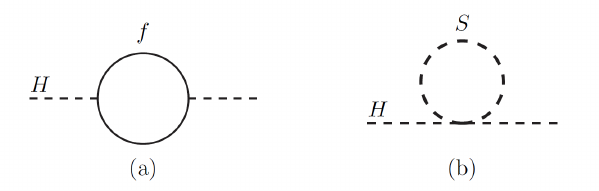
\includegraphics[scale=0.5]{Figure-1-One-loop-quantum-corrections-to-the-Higgs-squared-mass-parameter-m-2-H-from.png}
%\caption{The Feymann diagram for the one loop correction to the Higgs squared mass due to (a) a fermion $f$ and (b) a scalar $S$.
%The figure is taken from~\cite{Martin:1997ns}.}
%\label{fig:susy_one_loop_corrections}
%\end{center}
%\end{figure}
\begin{figure}[htbp]
    \begin{center}
        \begin{subfigure}[b]{0.48\textwidth}
            \begin{center}
                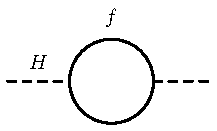
\includegraphics[scale=1]{one-loop-correction-1.pdf}
                \caption{}
            \end{center}
        \end{subfigure}%
        \begin{subfigure}[b]{0.48\textwidth}
            \begin{center}
                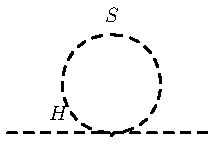
\includegraphics[scale=1]{one-loop-correction-2.pdf}
                \caption{}
            \end{center}
        \end{subfigure}
    \end{center}
    \caption{The Feymann diagram for the one loop correction to the Higgs squared mass due to (a) a fermion $f$ and (b) a scalar $S$.
    The figure is taken from~\cite{Martin:1997ns}.}
    \label{fig:susy_one_loop_corrections}
\end{figure}

The corrections are
%
\begin{align}
    \Delta m_{H}^{2} &= - \frac{|\lambda_{f}^{2}|}{8\pi^{2}} \Lambda_{UV}^{2} + \cdots, \quad \mathrm{fermion}\\
    \Delta m_{H}^{2} &= \frac{\lambda_{S}}{16\pi^{2}} \Lambda_{UV}^{2} + \cdots, \quad \mathrm{boson}
\end{align}
%
where the $\Lambda_{UV}$ is an ultraviolet momentum cutoff which is valid up to the Plank scale $10^{19}$~{\GeV}.
The corrections diverge when $\Lambda_{UV}$ becoming very large.
Because the contributions from the fermion and scalar loops have opposite sign, the divergence contributions can be canceled out if there is a scalar loop for each fermonic loop.
The SUSY predicts the existence of the bosonic/fermonic sparticles, therefore, if $\lambda_{S} = 2 |\lambda_{f}^{2}|$ then the SUSY maintain the finiteness of the Higgs squared mass in a natural way.

%%%
%%%
%%%

\subsubsection{Dark matter}
\label{subsubsec:susy_dark_matter}
The dark matter (DM) makes up about 27\% of the universe and it might originate from neutral relic from the early universe.
The cosmology observations of the DM indicate that the dark mater should be electrically neutral, cold, massive, and it participates only the weak and gravitational interactions.
Therefore, the DM candidate should be a new particle which is \textit{weakly interacting massive particle} (WIMP).
The SUSY requires all the sparticles must be produced in pairs and they decay into stable \textit{lightest SUSY particles} (LSP) with odd number.
If there are a lot of sparticles produced in the early Universe, they will have to decayed to LSPs and remain until the present day because the LSP is stable.
The LSP is a weakly interacting massive particle.
It doesn't interact electromagnetically so they cannot be scattered by photon and thus dark.
There are 3 kinds of LSP could be the possible DM candidate, the lightest \textit{neutralino}, the lightest \textit{sneutrino} and the \textit{gravitino}.

%%%
%%%
%%%

\subsubsection{Grand Unification}
\label{subsubsec:susy_gut}
The Grand Unified Theory (GUT) tries to unify the strong and electroweak interactions.
There will be only one interaction and one coupling constant at the GUT scale ($\approx 10^{16}$~{\GeV}).
However, the current coupling constants for electromagnetic, weak, and strong interactions don't unified at the GUT scale as shown in the left hand side of Fig.~\ref{fig:sm_coulping_constants}.
This problem can be solved by introducing the SUSY which modifies the renormalization group equations and make the running gauge couplings converged at the GUT scale.
The right hand side of Fig.~\ref{fig:sm_coulping_constants} shows the running gauge couplings in SUSY.

%%%
%%%
%%%

\section{Introduction of the supersymmetry}
\label{sec:susy_intro}
An brief overview of the SUSY are introduced in this section.
Firstly, the mathematical foundation of the SUSY, superalgebra, is described in Sect.~\ref{subsec:susy_superalgebra} followed by the superspace and superfields in Sect.~\ref{subsec:susy_superspace_and_superfields}.

%%%
%%%
%%%

\subsection{Superalgebra}
\label{subsec:susy_superalgebra}

%%%
%%%
%%%

\subsubsection{Poincar\'{e} algebra}
\label{subsubsec:susy_poincare}
The SUSY is based on the superalgebra which is an extension of space-time Poincar\'{e} algebra.
The Poincar\'{e} group is a product of the Lorentz group and the group of translations in space-time.
A Lorentz group must satisfies the commutation relations
%
\begin{equation}
    [J^{+}_{i}, J^{+}_{j}] = i \epsilon_{ijk} J^{+}_{k}, \quad 
    [J^{-}_{i}, J^{-}_{j}] = i \epsilon_{ijk} J^{-}_{k}, \quad 
    [J^{+}_{i}, J^{-}_{j}] = 0
    \label{eq:susy_Lorentz_commutation_relations}
\end{equation}
%
where $i, j, k = 1, 2, 3$.
If the six Lorentz group generators are combined into an antisymmetric second rank tensor generator $M_{\mu\nu}$ where $M_{ij} = \epsilon_{ijk}J_{k}$ and $M_{0i} = -M_{i0} = -K_{i}$\footnote{The $J_{i}$ and $K_{i}$ with $i=1,2,3$ are rotation and boost generators in 3-dimension respectively. And the ladder operators are defined as $J_{i}^{\pm} = \frac{1}{2} (J_{i} \pm i K_{i})$.} and the generator of the translation groups is $P_{\mu}$, the energy-momentum operator, then the commutation relations of the Poincar\'{e} group are
%
\begin{align}
    [P_{\mu}, P_{\nu}] &= 0 ,\\
    [M_{\mu \nu}, P_{\lambda}] &= i (g_{\nu \lambda} P_{\mu} - g_{\mu \lambda} P_{\nu}) ,\\
    [M_{\mu \nu}, M_{\rho \sigma}] &= -i (g_{\mu \rho} M_{\nu \sigma} - g_{\mu \sigma} M_{\nu \rho} - g_{\nu \rho} M_{\mu \sigma} + g_{\nu \sigma} M_{\mu \rho}) .
    \label{eq:susy_Poincare_commutation_relations}
\end{align}
%
where the metric is 
\begin{equation}
    g_{\mu \nu} =
    \left(
        \begin{array}{cccc}
            1 & 0  & 0  & 0\\
            0 & -1 & 0  & 0\\
            0 & 0  & -1 & 0\\
            0 & 0  & 0  & -1   
        \end{array}
    \right)
    \label{eq:susy_metric}
\end{equation}
%

%%%
%%%
%%%

\subsubsection{Spinor}
\label{subsubsec:susy_spinor}
A general spin $\frac{1}{2}$ particle state, $\chi$, can be expressed as a \textit{spinor} in the SUSY using two-component spin up $\chi_{+}$ and spin down $\chi_{-}$ column matrices
%
\begin{equation}
    \chi = c_{+} \chi_{+} + c_{-} \chi_{-}
    = c_{+} \left(\begin{matrix}1\\0\end{matrix}\right) + c_{-} \left(\begin{matrix}0\\1\end{matrix}\right)
    = \left(\begin{matrix}c_{+}\\c_{-}\end{matrix}\right)
    \label{eq:susy_spinor}
\end{equation}
%
The solution of the Dirac equation\footnote{The Dirac equation is $(i \gamma^{\mu} \partial_{\mu} - m)\psi = 0$.}, $\psi_{D}\footnote{The Dirac spinor $\psi_{D}$ is a four-component field which can be expressed using a four-component matrix.}$, can be expressed using the left-handed and right-handed \textit{Weyl spinors} $\psi_{L}$ and $\psi_{R}$ 
%
\begin{equation}
    \psi_{D} = \left(\begin{matrix}\psi_{1}\\\psi_{2}\\\psi_{3}\\\psi_{4}\end{matrix}\right)
    = \left(\begin{matrix} \left(\begin{matrix}\psi_{1}\\\psi_{2}\end{matrix}\right) \\ \left(\begin{matrix}\psi_{3}\\\psi_{4}\end{matrix}\right) \end{matrix}\right)
    = \left(\begin{matrix}\psi_{L}\\\psi_{R}\end{matrix}\right)
    \label{eq:susy_Dirac_spinor}
\end{equation}
%
It is convenient to use the Weyl spinors to represent the building blocks for any fermion field.
The Majorana spinor $\tilde{\psi}_{M}$ is a real solution of Dirac equation.
It is its own charge conjugate and satisfies the Majorana condition
%
\begin{equation}
    \tilde{\psi}_{M} = \tilde{\psi}_{M}^{*}
    \label{eq:susy_majorana_condition}
\end{equation}
%
The Majorana spinor can be expressed in terms of the Weyl spinors
%
\begin{equation}
    \psi_{M} = \left(\begin{matrix}\xi_{\alpha}\\\bar{\xi}^{\dot{\alpha}}\end{matrix}\right)
    %= \left(\begin{matrix}\xi_{\alpha}\\0\end{matrix}\right) + \left(\begin{matrix}0\\\bar{\xi}^{\dot{\alpha}}\end{matrix}\right)
    %= \psi_{W,L} + \psi_{W,R}
    \label{eq:susy_majorana_spinor}
\end{equation}
%
where the left-handed Weyl spinor $\xi_{\alpha}$ and the right-handed Weyl spinor $\bar{\xi}^{\dot{\alpha}}$ are the Hermitian conjugate of each other.

%%%
%%%
%%%

\subsubsection{Helicity}
\label{subsubsec:susy_helicity}
A particle with momentum $\vec{p}$ and angular momentum $\vec{J}$, then the \textit{helicity} is defined as
%
\begin{equation}
    h = \vec{J} \cdot \hat{p} = (\vec{L} + \vec{S}) \cdot \hat{p} = \vec{S} \cdot \hat{p}, \quad \hat{p} = \frac{\vec{p}}{|\vec{p}|}
    \label{eq:susy_helicity}
\end{equation}
%
The eigenvalues of $h$ are +1 and -1 corresponding to right-handed and and left-handed eigenstates.
Although the helicity is rotation invariant but not boost invariant, the helicity of a massless particle moving at the speed of light is Lorentz invariant.

%%%
%%%
%%%

\subsection{Superspace and superfields}
\label{subsec:susy_superspace_and_superfields}
The superspace is composed of the ordinary space-time coordinate and four anticommuting fermonic coordinates $\theta_{\alpha}$ and $\bar{\theta}_{\dot{\alpha}}$ where the spinor indices $\alpha$ and $\dot{\alpha}$ can be 1 or 2. 
A superfield $S(x^{\mu}, \theta_{\alpha}, \bar{\theta}_{\dot{\alpha}})$ is a function in superspace.
The general form of a superfield can be expressed in terms of $\theta$ and $\bar{\theta}$
%
\begin{equation}
    S(x, \theta, \bar{\theta}) = a + \theta \xi + \bar{\theta} \bar{\chi} + \theta \theta b + \bar{\theta}\bar{\theta}c + \bar{\theta}\bar{\sigma}^{\mu}\theta v_{\nu} + \theta \theta \bar{\theta} \bar{\zeta} + \bar{\theta} \bar{\theta} \theta \eta + \theta \theta \bar{\theta} \bar{\theta} d
    \label{eq:susy_superfield}
\end{equation}
%
where all spinor indices are suppressed.
The $a, b, c, d$, and $v_{\mu}$ are bosonic fields and $\xi, \bar{\chi}, \bar{\zeta}, \eta$ are fermonic fields which are complex functions of $x^{\mu}$.
The SUSY generators $Q_{\alpha}$ and $\bar{Q}_{\dot{\alpha}}$ can be expressed as
%
\begin{equation}
    Q_{\alpha} = -i \frac{\partial}{\partial \theta^{\alpha}} - \sigma^{\mu}_{\alpha \dot{\beta}} \bar{\theta}^{\dot{\beta}} \partial_{\mu}, \quad
    \bar{Q}_{\dot{\alpha}} = i \frac{\partial}{\partial \bar{\theta}^{\dot{\alpha}}} + \theta^{\beta} \sigma^{\mu}_{\beta \dot{\alpha}} \partial_{\mu}
    \label{eq:susy_susy_generators}
\end{equation}
%
and the commutation relations are
%
\begin{equation}
    \{Q_{\alpha}, \bar{Q}_{\bar{\beta}}\} = -2i \sigma^{\mu}_{\alpha \dot{\beta}} \partial_{\mu}, \quad
    \{Q_{\alpha}, Q_{\beta}\} = \{\bar{Q}_{\dot{\alpha}}, \bar{Q}_{\dot{\beta}}\} = 0
    \label{eq:susy_susy_generator_commutation_relations}
\end{equation}
%
The SUSY covariant derivatives are defined as
%
\begin{equation}
    D_{\alpha} = \frac{\partial}{\partial \theta^{\alpha}} + i \sigma^{\mu}_{\alpha \dot{\beta}} \bar{\theta}^{\dot{\beta}} \partial_{\mu}, \quad
    \bar{D}_{\dot{\alpha}} = (D_{\alpha})^{\dagger} = \frac{\partial}{\partial \bar{\theta}^{\dot{\alpha}}} + i \theta^{\beta} \sigma^{\mu}_{\beta}{\dot{\alpha}} \partial_{\mu}
    \label{eq:susy_susy_covariant_derivatives}
\end{equation}
%
and the commutation relations are
%
\begin{equation}
    \{D_{\alpha}, \bar{D}_{\bar{\beta}}\} = 2i \sigma^{\mu}_{\alpha \dot{\beta}} \partial_{\mu}, \quad
    \{D_{\alpha}, D_{\beta}\} = \{\bar{D}_{\dot{\alpha}}, \bar{D}_{\dot{\beta}}\} = 0
    \label{eq:susy_susy_covariant_derivatives_commutation_relations}
\end{equation}
%
The SUSY covariant derivatives anticommute with the SUSY generators\footnote{$\{D_{\alpha}, Q_{\beta}\} = \{D_{\alpha}, \bar{Q}_{\dot{\beta}}\}= \{\bar{D}_{\dot{\alpha}}, Q_{\beta}\} = \{\bar{D}_{\dot{\alpha}}, \bar{Q}_{\dot{\beta}}\} =0$}.

%%%
%%%
%%%

\subsubsection{Chiral superfields and vector superfields}
\label{subsec:susy_chiral_superfields_and_vector_superfields}
The spin 0 bosons and spin 1/2 fermions are described using the \textit{chiral superfield} and the spin 1 gauge bosons are described using the \textit{vector superfields}. $V(x, \theta, \bar{\theta})$.
The chiral superfield, $\Phi(x, \theta, \bar{\theta})$, satisfies the condition\footnote{The antichiral superfield satisfies $D_{\alpha}\Phi^{*} = 0$ where $\Phi^{*}$ is the complex conjugate of $\Phi$.}
%
\begin{equation}
    \bar{D}_{\dot{\alpha}} \Phi = 0
    \label{eq:susy_chiral_superfield_condition}
\end{equation}
%
If we redefine the new coordinates $(y^{\mu}, \theta)$ and $(\bar{y}^{\mu}, \bar{\theta})$ in the superface\footnote{The chiral coordinate is $(y^{\mu}, \theta)$ and the antichiral coordinate is $(\bar{y}^{\mu}, \bar{\theta})$},
%
\begin{equation}
    y^{\mu} = x^{\mu} + i \theta \sigma^{\mu} \bar{\theta}, \quad \bar{y}^{\mu} = x^{\mu} - i \theta \sigma^{\mu} \bar{\theta}
    \label{eq:susy_chiral_coordinate}
\end{equation}
%
then the covariant derivatives become
%
\begin{equation}
    D_{\alpha} = \frac{\partial}{\partial \theta^{\alpha}} + 2i \sigma^{\mu}_{\alpha \dot{\beta}} \bar{\theta}^{\dot{\beta}} \frac{\partial}{\partial y^{\mu}}, \quad \bar{D}_{\dot{\alpha}} = \frac{\partial}{\partial \bar{\theta}^{\dot{\alpha}}}
    \label{eq:susy_chiral_covariant_derivative}
\end{equation}
%
And the general form of a chiral superfield can be expressed in terms of the chiral coordinate $(y^{\mu}, \theta)$ only
%
\begin{equation}
    \Phi(y, \theta) = \phi(y) + \sqrt{2} \theta \psi(y) + \theta \theta F(y)
    \label{eq:susy_chiral_superfield_general_form}
\end{equation}
%
The vector superfield, $V$, is a real field\footnote{The vector superfield satisfies $V(x, \theta, \bar{\theta}) = V^{\dagger}(x, \theta, \bar{\theta})$.} and the general form is
%
\begin{align}
    V(x, \theta, \bar{\theta}) &= C + i \theta \chi - i \bar{\theta} \bar{\chi} + \theta \sigma^{\mu} \bar{\theta} v_{\mu} + \frac{i}{2} \theta \theta (M + iN) - \frac{i}{2} \bar{\theta} \bar{\theta}(M - iN)\\
    &+ i \theta \theta \bar{\theta} (\bar{\lambda} + \frac{i}{2} \bar{\sigma}^{\mu} \partial_{\mu} \chi) - i \bar{\theta} \bar{\theta} \theta (\lambda - \frac{i}{2} \sigma^{\mu} \partial_{\mu} \bar{\chi}) + \frac{1}{2} \theta \theta \bar{\theta} \bar{\theta} (D - \frac{1}{2} \partial^{2} C)
    \label{eq:susy_vector_superfield_general_form}
\end{align}
%
where the $C, M, N, D$ are real scalars, the $\chi, \lambda$ are Weyl spinors, and the $v_{\mu}$ is a vector field.
By applying the Wess-Zumino gauge, the general form can be reduced into
%
\begin{equation}
    V_{WZ} = \theta \sigma^{\mu} \bar{\theta} v_{\mu} + i \theta \theta \bar{\theta} \bar{\lambda} - i \bar{\theta} \bar{\theta} \theta \lambda + \frac{1}{2} \theta \theta \bar{\theta} \bar{\theta} D
    \label{eq:susy_vector_superfield_reduced_form}
\end{equation}
%
The non-vanishing power of $V_{WZ}$ is $V^{2}_{WZ} = \frac{1}{2} \theta \theta \bar{\theta} \bar{\theta} v_{\mu} v^{\mu}$.
All the higher power of $V_{WZ}$ are all vanishing $V^{n}_{WZ} = 0, n \ge 3$.

%%%
%%%
%%%

\subsection{$R$-parity}
\label{subsec:susy_r_parity}
The baryon number $B$ and lepton number $L$ are conserved in the SM but violated in the SUSY.
Therefore, a new symmetry called $R$-parity is introduced to eliminate the $B$ and $L$ violating term.
The $R$-parity is defined as
%
\begin{equation}
    R \equiv (-1)^{3(B-L)+2s}
    \label{eq:susy_r_parity}
\end{equation}
%
where $s$ is the spin of the particle.
All of the SM particles have even $R$-parity ($R$ = +1), while all of the sparticles have odd $R$-parity ($R$ =  1). 
If the $R$-parity is conserved, SUSY predicts that sparticles are produced in pairs in collider experiments.

%%%
%%%
%%%

\subsection{Suppersymmetry breaking}
\label{sybsec:susy_soft_susy_breaking}
The supermultiplets are the single particle states in SUSY theory and it corresponds to the irreducible representations of the super-Poincar\'{e} algebra.
A supermultiplet contains boson and fermion with the same degrees of freedom and all particles in the same supermultiplet have the same mass.
However, no any sparticles have been observed from the experiments.
Therefore, the SUSY must be spontaneously broken and the sparticles must be heavier than their SM partners.
The scalar superpotential $V$ can be represented by the auxiliary fields $F_{i}$ and $D_{a}$
%
\begin{equation}
    V = F^{*i}F_{i} + \frac{1}{2} \sum_{a} D^{a} D_{a}
    \label{eq:susy_scalar_superpotential}
\end{equation}
%
A state $|\Omega \rangle$ is called a vacuum state if $E_{\Omega} = \langle \Omega | H | \Omega \rangle = 0$.
This happens when the potential $V$ has a minimum.
There are two kinds of vacuums, the true vacuum and the false vacuum which correspond to the global minimum and the local minimum of the scalar potential $V$, respectively.
For example, when $F_{i} = D_{a} = 0$, then $V = 0$ is a global minimum.
The $\langle F \rangle = 0$ is called $F$-term breaking and the $\langle D \rangle = 0$ is called $D$-term breaking.

%%%
%%%
%%%

\subsection{The Minimal Supersymmetry Standard Model}
\label{subsec:susy_mssm}
The Minimal Supersymmetry Standard Model (MSSM) is the minimal extension of the Standard Model.
The MSSM contains only the smallest number of superfields and interactions such that the SM particles can keep their current forms.

%%%
%%%
%%%

\subsubsection{Particle content}
\label{subsubsec:susy_particle_content}
All the super particles, \textit{\textbf{s}particles}\footnote{The super particles of the SM fermions are prefix a "\textit{\textbf{s}}" and the super particles of the SM bosons are suffix an "\textit{\textbf{ino}}". A tilde is added on the symbol of the SM particle to denote its super partner.}, have exactly the same quantum number as their SM particles except the spins differ by $\frac{1}{2}$.
The super partners of the leptons and quarks are called \textit{\textbf{s}leptons} and \textit{\textbf{s}quarks}.
The sleptons and squarks are scalar particles with spin $s=0$ and the left-handed and right-handed states are treated as different particles such that the SM particles and the SUSY \textbf{s}particles have the same number of degree of freedom.
The super partners of gluons are \textit{glu\textbf{ino}s} and there are eight gluinos with spin $s=\frac{1}{2}$. 
The super partners of the gauge bosons $W^{\pm}, Z^{0}$, and $\gamma$, are \textit{gaug\textbf{ino}s}.
The gauginos have spin $s = \frac{1}{2}$.
The super partners of the Higgs bosons\footnote{The Higgs sector contains two charged states $H^{\pm}$ and three neutral states $h^{0}, H^{0}$, and $A^{0}$. The $h^{0} and H^{0}$ are $CP$ even state and $A^{0}$ is $CP$ odd state.} are \textit{Higgs\textbf{ino}s}.
The Higgsinos and gauginos mixing states are two \textit{charginos} $\tilde{\chi}_{1}^{\pm}, \tilde{\chi}_{2}^{\pm}$ and four \textit{neutralinos} $\tilde{\chi}_{1}^{0}, \tilde{\chi}_{2}^{0}, \tilde{\chi}_{3}^{0}, \tilde{\chi}_{4}^{0}$ with spin $s=\frac{1}{2}$.
Table~\ref{tab:susy_particle_contents} shows the particle contents in the MSSM.

\begin{table}[htp]
    %\begin{center}
    \resizebox{\textwidth}{!}{% <------ Don't forget this %
        \begin{tabular}{ccccccc}
            \hline
            \hline
            Supermultiplet          & Names                                                      & Symbol         & spin 0                                           & spin 1/2                                               & spin 1 & $SU(3)_{C} \otimes SU(2)_{L} \otimes U(1)_{Y}$\\
            \hline
            \multirow{3}{*}{Chiral} & \multirow{3}{3cm}{squarks, quarks ($\times 3$ families)}   & Q              & ($\widetilde{u}_{L}$, \quad $\widetilde{d}_{L})$ & $(u_{L}, \quad d_{L})$                                 & -                  & $\mathbf{3} \otimes \mathbf{2}\otimes \frac{1}{6}$\\
                                    &                                                            & $\overline{u}$ & $\widetilde{u}^{*}_{R}$                          & $u^{\dag}_{R}$                                         & -                  & $\overline{\mathbf{3}} \otimes \mathbf{1} \otimes -\frac{2}{3}$\\
                                    &                                                            & $\overline{d}$ & $\widetilde{d}^{*}_{R}$                          & $d^{\dag}_{R}$                                         & -                  & $\overline{\mathbf{3}} \otimes \mathbf{1} \otimes \frac{1}{3}$\\
            \hline
            \multirow{2}{*}{Chiral} & \multirow{2}{3cm}{sleptons, leptons ($\times 3$ families)} & L              & $(\widetilde{\nu}, \quad \widetilde{e}_{L})$     & $(\nu, \quad e_{L})$                                   & -                  & $\mathbf{1} \otimes \mathbf{2} \otimes -\frac{1}{2}$\\
                                    &                                                            & $\overline{e}$ & $\widetilde{e}^{*}_{R}$                          & $e^{\dag}_{R}$                                         & -                  & $\mathbf{1} \otimes \mathbf{1} \otimes 1$\\
            \hline
            \multirow{2}{*}{Chiral} & \multirow{2}{*}{Higgs, higgsinos}                          & $H_{u}$        & $(H^{+}_{u}, \quad H^{0}_{u})$                   & $(\widetilde{H}^{+}_{u}, \quad \widetilde{H}^{0}_{u})$ & -                  & $\mathbf{1} \otimes \mathbf{2} \otimes +\frac{1}{2}$\\
                                    &                                                            & $H_{d}$        & $(H^{0}_{d}, \quad H^{-}_{d})$                   & $(\widetilde{H}^{0}_{d}, \quad \widetilde{H}^{-}_{d})$ & -                  & $\mathbf{1} \otimes \mathbf{2} \otimes -\frac{1}{2}$\\
            \hline
            \hline
            \multirow{3}{*}{Gauge}  & gluino, gluon                                              & -              & -                                                & $\widetilde{g}$                                        & $g$                & $\mathbf{8} \otimes \mathbf{1} \otimes 0$\\
                                    & winos, $W$ bosons                                          & -              & -                                                & $\widetilde{W}^{\pm}$, $\widetilde{W}^{0}$             & $W^{\pm}$, $W^{0}$ & $\mathbf{1} \otimes \mathbf{3} \otimes 0$\\
                                    & bino, $B$ boson                                            & -              & -                                                & $\widetilde{B}^{0}$                                    & $B^{0}$            & $\mathbf{1} \otimes \mathbf{1} \otimes 0$\\
            \hline
            \hline
        \end{tabular}
    }
    %\end{center}
    \caption{Chiral supermultiplets and gauge supermultiplets in the MSSM.
    In the chiral supermultiplets, the spin 0 fields are complex scalars and the spin 1/2 fields are left-handed two-component Weyl spinors.}
    \label{tab:susy_particle_contents}
\end{table}%

%%%
%%%
%%%

\section{The radiative natural SUSY}
\label{sec:susy_rns}
The radiative natural SUSY (RNS)~\cite{Baer:2013xua, Baer:2012up, Baer:2012se, Baer:2012cf} is based on MSSM and it may be vaild all the way up to the GUT scale\footnote{The GUT scale is about $m_{\text{GUT}} \approx 2 \times 10^{16}$~{\GeV}.}.
The RNS maintains the Higgs mass \mH $\sim 125$~{\GeV} and $Z$ boson mass \mZ = 91.2~{\GeV} and requires no large cancellations at the electroweak scale.
It also expects the light higgsino masses to be 100 $\sim$ 300~{\GeV}, the electroweak gaugino masses 300 $\sim$ 1200~{\GeV}, the masses of $\tilde{g}$, $\tilde{t}$, and $\tilde{b}$ to be 1 $\sim$ 4~{\TeV}, and the masses of $\tilde{u}$, $\tilde{d}$, $\tilde{s}$, $\tilde{c}$ exist in the 5 $\sim$ 30~{\TeV} range.

In SUSY models, the $Z$ boson mass can be obtained from the minimization condition on the Higgs sector scalar potential
%
\begin{equation}
    \frac{m_{Z}^{2}}{2} = \frac{m^{2}_{H_{d}} + \Sigma^{d}_{d} - (m^{2}_{H_{u}} + \Sigma^{u}_{u})\tan^{2}\beta      }{\tan^{2}\beta - 1} - \mu^{2}
    \label{eq:susy_minimization_condition}
\end{equation}
%
where $\Sigma^{d}_{d}$ and $\Sigma^{u}_{u}$ are ratiative corrections including the contributions from various particles and sparticles Yukawa and gauge coulpings to the Higgs sector.
Requiring no large cancellations means each term on the right-hand-side of Eq.~(\ref{eq:susy_minimization_condition}) are individually comparable to the left-hand-side, $m_{Z}^{2}/2$.
Therefore, no large electroweak fine-tuning (EWFT) is required to obtain \mZ = 91.2~{\GeV} and leads to a model with electroweak naturalness.
The EWFT parameter is defined as
%
\begin{equation}
    \Delta_{EW} =  max_{i} \frac{|C_{i}|}{(m_{Z}^{2}/2)} 
    \label{eq:susy_ewft}
\end{equation}
%
which depends only on the weak scale parameters of the theory.
Low $\Delta_{EW}$ value means less fine-tuning.
For example, $\Delta_{EW} = 10 \sim 30$ correspond to $3 \sim 10 \%$ fine-tuning.
The $C_{i}$ represents $C_{H_{d}}$, $C_{H_{u}}$, $C_{\mu}$, $C_{\Sigma^{d}_{d}(k)}$, and $C_{\Sigma^{u}_{u}(k)}$
%
\begin{align}
    C_{H_{d}} &= \frac{m^{2}_{H_{d}}}{\tan^{2}\beta - 1}\\
    C_{H_{u}} &= \frac{-m^{2}_{H_{u}}\tan^{2}\beta}{\tan^{2}\beta - 1}\\
    C_{\mu} &= -\mu^{2}\\
    C_{\Sigma^{d}_{d}(k)} &= \frac{\Sigma^{d}_{d}}{\tan^{2}\beta - 1}\\
    C_{\Sigma^{u}_{u}(k)} &= \frac{-\Sigma^{u}_{u}\tan^{2}\beta}{\tan^{2}\beta - 1}
    \label{eq:susy_ci}
\end{align}
% 
where $k$ denotes the various loop contributions included in Eq.~(\ref{eq:susy_minimization_condition}).
In order to get a small EWFT value, $\Delta_{EW} \leq 30$, the RNS has to satisfy
%
\begin{itemize}
    \item The light higgsino mass $100 < |\mu| < 300$~{\GeV}. 
    \item $m_{H_{u}}(m_{\text{GUT}}) \sim (1.3 \sim 2) m_{0}$. This leads to $m^{2}_{H_{u}} \sim - \frac{m^{2}_{Z}}{2}$ at the weak scale.
    \item $A_{0} \sim \pm 1.6 m_{0}$. This results in large radiative corrections of $\widetilde{t}_{i}$ whilst maintain \mH to the $\sim$125~{\GeV}.
\end{itemize}
%
In the RNS framework, which allows fine-tining at 5 $\sim$ 10\% level, the masses of the higgsino-like gauginos $\widetilde{\chi}^{\pm}_{1}$, $\widetilde{\chi}^{0}_{1}$, and $\widetilde{\chi}^{0}_{2}$ lie in 100 to 300~{\GeV} and the mass gap between $\widetilde{\chi}^{0}_{2}$ and $\widetilde{\chi}^{0}_{1}$ is 10 $\sim$ 30~{\GeV}.
The masses of third generation squarks are $m_{\widetilde{t}_{1}} \sim 1$ to 2~{\TeV} and $m_{\widetilde{t}_{2}}$, $m_{\widetilde{b}_{1}} \sim 2$ to 4~{\TeV}.
The gluino mass, $m_{\widetilde{g}}$, is about 1 to 5~{\TeV} and the masses of first and second generation sferminos, $m_{\widetilde{q}}, m_{\widetilde{\ell}}$, are about 5 to 10~{\TeV}.
And the light Higgs scalar mass is keeping at 125~{\GeV}.
The typical mass spectra of RNS is shown in Fig.~\ref{fig:susy_RNS_mass_spectra}.
The $m_{\widetilde{t}_{1,2}}$ and $m_{\widetilde{b}_{1,2}}$ are typically beyond 1~{\TeV} in the RNS, so it is very difficult to detect at LHC.  
The light higgsino-like charginos $\widetilde{\chi}^{\pm}_{1}$ and neutralinos $\widetilde{\chi}^{0}_{1,2}$ have substantial production cross-section in the RNS, these particles are produced at large rates at LHC.
Because the small mass splittings $\Delta m(\widetilde{\chi}^{\pm}_{1}, \widetilde{\chi}^{0}_{1})$ and $\Delta m(\widetilde{\chi}^{0}_{2}, \widetilde{\chi}^{0}_{1})$, the visible decay products tend to be at very low energies and will be hard to detect above the SM background, making the large \met.


\begin{figure}[htb]
    \begin{center}
        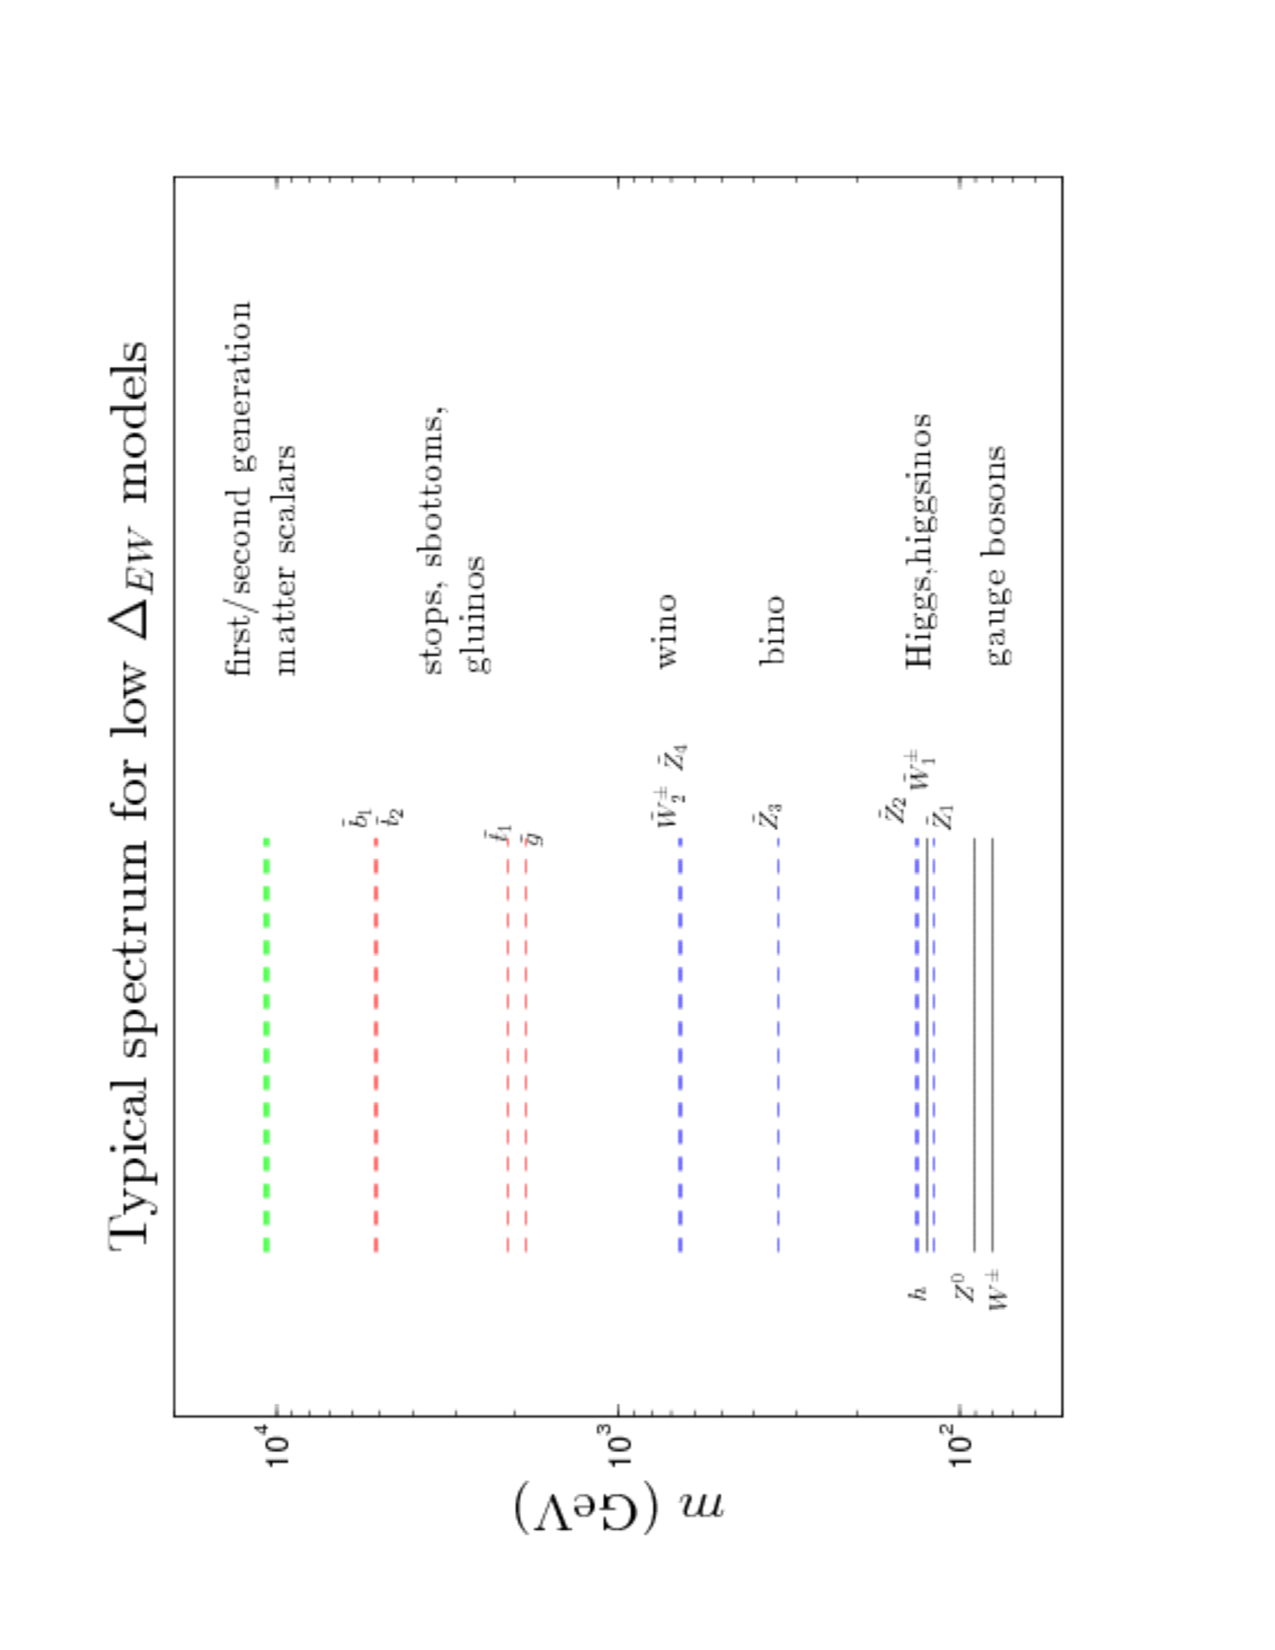
\includegraphics[scale=0.45,angle=270]{mass_hierarchy_xerxes_not.pdf}
        \caption{Typical sparticle mass spectra of RNS.
        The figure is taken from~\cite{Baer:2013gva}.}
        \label{fig:susy_RNS_mass_spectra}
    \end{center}
\end{figure}

%%%
%%%
%%%

\section{The non-universal Higgs model with two extra parameters}
\label{sec:susy_nuhm2}
The RNS can be generated from SUSY GUT type models using non-universal Higgs masses model with two extra parameters (NUHM2)~\cite{Ellis:2002wv, Ellis:2002iu, Baer:2004fu, Baer:2005bu} leading to a low fine-tuning $\Delta_{EW}$ value at the electroweak scale and keeping electroweak naturalness.
The NUHM2 decouples the Higgs mass dobelet parameters $m^{2}_{H_{u}}$ and $m^{2}_{H_{d}}$ at the GUT scale such that
%
\begin{equation}
    m^{2}_{H_{u}} \neq m^{2}_{H_{d}} \neq m^{2}_{0}(m_{\text{GUT}})
    \label{eq:susy_nuhm2_decouple}
\end{equation}
%
and it usually uses the weak scale parameters $\mu$ and $m_{A}$ to replace the $m^{2}_{H_{u}}$ and $m^{2}_{H_{d}}$.
%
\begin{align}
    \mu^{2} &= \frac{m^{2}_{H_{d}} - m^{2}_{H_{u}}\tan^{2}\beta}{\tan^{2}\beta - 1} - \frac{m^{2}_{Z}}{2}\\
    m^{2}_{A} &= m^{2}_{H_{d}} + m^{2}_{H_{u}} + 2\mu^{2}
    \label{eq:susy_weak_scale_parameters}
\end{align}
%
If the value of NUHM2 free parameters are chosen as the following ranges
%
\begin{itemize}
    \item The matter scalar mass $m_{0} \sim 1$ to 7~{\TeV},
    \item The soft SUSY breaking gaugino mass $m_{1/2} \sim 0.3$ to 1.5~{\TeV},
    \item The trilinear SUSY breaking parameter $A_{0} \sim \pm(1$ to $2) m_{0}$,
    \item The  ratio of the Higgs field vacuum expectation value $\tan\beta \sim 5$ to 50,
    \item The superpotential Higgs mass $\mu \sim 100$ to 300~{\GeV},
    \item The pseudoscalar Higgs boson mass $m_{A}$ is varied.
\end{itemize}
%
then the low EWFT can be achieved whilst remaining SUSY spectrum and maintaining $123 < \mH < 127$~{\GeV}.
Comparing with the well-known mSUGRA/CMSSM models which have the lowest $\Delta_{EW} \sim 200$, the $\Delta_{EW}$ in the NUHM2 model is about 10 only.
The NUHM2 is expected to form the the effective theory for energies lower than $m_{GUT}$ resulting from $SU(5)$ or general $SO(10)$ grand unified theories.
Detailed scans for the NUHM2 parameter space with low EWFT had been performed in~\cite{Baer:2013xua}, and the NUHM2 parameter values used in this analysis are set to $m_{0} = 5$~{\TeV}, $A_{0} = -1.6 m_{0}$, $\tan\beta = 15$, $m_{A} = 1$~{\TeV}, $\mu = 150$ such that sign($\mu$) $> 0$, and $m_{1/2}$ are varied from 350 to 800~{\GeV}.
These parameter choices lead to low EWFT (electroweak naturalness) and predict final state signatures that allow large background rejection while retaining high signal efficiency.
Although the kinematics of NUHM2 are very similar to the simplified Higgsino model in compressed scenarios, the primary differences are resulting from the mass spectra, cross-sections, and branching ratios between NUHM2 and simplified Higgsino model.

\begin{figure}[htb]
    \begin{center}
        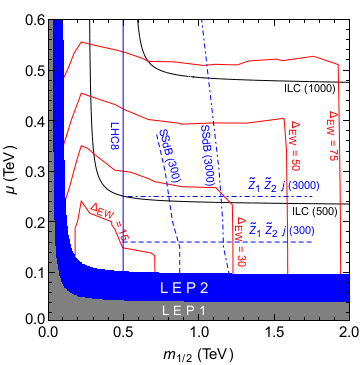
\includegraphics[scale=0.7]{mumhf.png}
        \caption{The $\Delta_{EW}$ contours in the $m_{1/2}$ vs $\mu$ plane of NUHM2 model for $m_{0} =  5$~{\GeV}, $\tan\beta = 15$, $A_{0} = -1.6 m_{0}$, and $m_{A} = 1$~{\TeV}.
        The gray and blue shaded regions are excluded by the LEP1 and LEP2 searches for chargino pair production.
        The region on the left hand side of the blue solid line is excluded by LHC8 gluino pair searches.
        This figure is taken from~\cite{Baer:2016usl}.}
        \label{fig:susy_mumhf}
    \end{center}
\end{figure}

Figure~\ref{fig:susy_mumhf} shows the $m_{1/2}$ vs $\mu$ plane of NUHM2 model for $m_{0} =  5$~{\GeV}, $\tan\beta = 15$, $A_{0} = -1.6 m_{0}$, and $m_{A} = 1$~{\TeV}.
The gray and blue regions are excluded by searches for chargino pair production at LEP1 and LEP2.
The area to the left of the blue solid line is excluded by the $\widetilde{g} \widetilde{g}$ production at LHC with $\sqrt{s} = 8$~{\TeV}.
The contours for $\Delta_{EW} = 15, 30, 50, 70$ are shown.
The $\widetilde{\chi}^{0}_{2} \widetilde{\chi}^{0}_{1}$ with one ISR jet production where $\widetilde{\chi}^{0}_{2} \to \ell^{+} \ell^{-} \widetilde{\chi}^{0}_{1}$ is labeled by two horizontal dashed contours at 300 \ifb and 3000 \ifb, respectively\footnote{The $\widetilde{\chi}^{0}_{1}$ is indicated by $\widetilde{Z}_{1}$ and the $\widetilde{\chi}^{0}_{2}$ is indicated by $\widetilde{Z}_{2}$ in the plot.}.
The $\widetilde{\chi}^{0}_{2} \widetilde{\chi}^{0}_{1}$ with one ISR jet is accessible in nearly the entire $\Delta_{EW} < 30$ region.
For comparison, the reach of International Linear Collider (ILC) with $\sqrt{s} = 0.5$ and 1~{\TeV} are shown.
Thus, the RNS, which accommodates the electroweak naturalness, can be either discovered or ruled out by the LHC plus ILC searches.



\chapter{The ATLAS Experiment at LHC}
\label{chapter:altas_experiment}
\graphicspath{{figures/atlas_experiment/}}
The European Organization for Nuclear Research (CERN\footnote{The name CERN is derived from the acronym for the French Conseil Europ\'{e}en pour la Recherch Nucl\'{e}aire}) was founded in 1954 and is based in the suburb of Geneva on the Franco\textendash Swiss border.
The main function of CERN is to provide particle accelerators and detectors for high-energy physics research.
The physicists and engineers at CERN are probing the fundamental structure of the universe using the world's largest and most complex scientific facility \textemdash \ the Large Hadron Collider (LHC)~\cite{1748-0221-3-08-S08001}.
In the LHC, the particles are boosted to high energies and collide at close to the speed of light.
The results of the collisions are recorded by the various detectors.
There are seven experiments at the LHC.
The biggest of these experiments are ATLAS (A Toroidal LHC ApparatuS)~\cite{1748-0221-3-08-S08003} and CMS (Compact Muon Solenoid)~\cite{1748-0221-3-08-S08004} which use general-purpose detectors to investigate a broad physics programme ranging from the search for the Higgs boson to extra dimensions and particles that could make up dark matter.
The ALICE (A Large Ion Collider Experiment)~\cite{1748-0221-3-08-S08002} experiment is designed to study the physics of quark-gluon plasma form and the LHCb (Large Hadron Collider beauty)~\cite{1748-0221-3-08-S08005} experiment specializes in investigating of CP violation by studying the $b$-quark.
These four detectors sit underground in huge caverns of the LHC ring.
The rest three experiments, TOTEM~\cite{1748-0221-3-08-S08007}, LHCf~\cite{1748-0221-3-08-S08006}, and MoEDAL~\cite{Pinfold:1181486}, are smaller.
The TOTEM (TOTal Elastic and diffractive cross section Measurement)~\cite{1748-0221-3-08-S08007} experiment aims at the measurement of total cross section, elastic scattering, and diffractive dissociation.
The LHCf (Large Hadron Collider forward)~\cite{1748-0221-3-08-S08006} experiment is intended to measure the neutral particle produced by the collider using the forward particles.
The prime motivation of the MoEDAL (Monopole and Exotics Detector at the LHC)~\cite{Pinfold:1181486} experiment is to search directly for the magnetic monopole.

\section{The Large Hadron Collide}

The LHC~\cite{1748-0221-3-08-S08001} is the world's largest and most powerful accelerator which accelerates and collides protons in a 26.7~km circumference crossing the Franco\textendash Swiss border 100 m underground.
Built in the tunnel of the former LEP (Large Electron\textendash Positron), the LHC is capable of colliding protons as well as heavy ions.
Comparing with the LEP which collides electrons and positrons, the advantage of the LHC is the lower energy loss \footnote{The energy loss for protons is about eleven orders of magnitude smaller than the electrons} in the synchrotron radiation, such that higher energies can be reached by the LHC.
The LHC is designed for collisions at a centre-of-mass energy $\sqrt{s}=14$~{\TeV} and an instantaneous luminosity of $\mathcal{L} =10^{34}~\textrm{cm}^{-2}\textrm{s}^{-1}$.
Figure~\ref{fig:CERN_accelerator_complex} shows the infrastructure of the LHC and the pre-accelerator system.

\begin{figure}[htbp]
\begin{center}
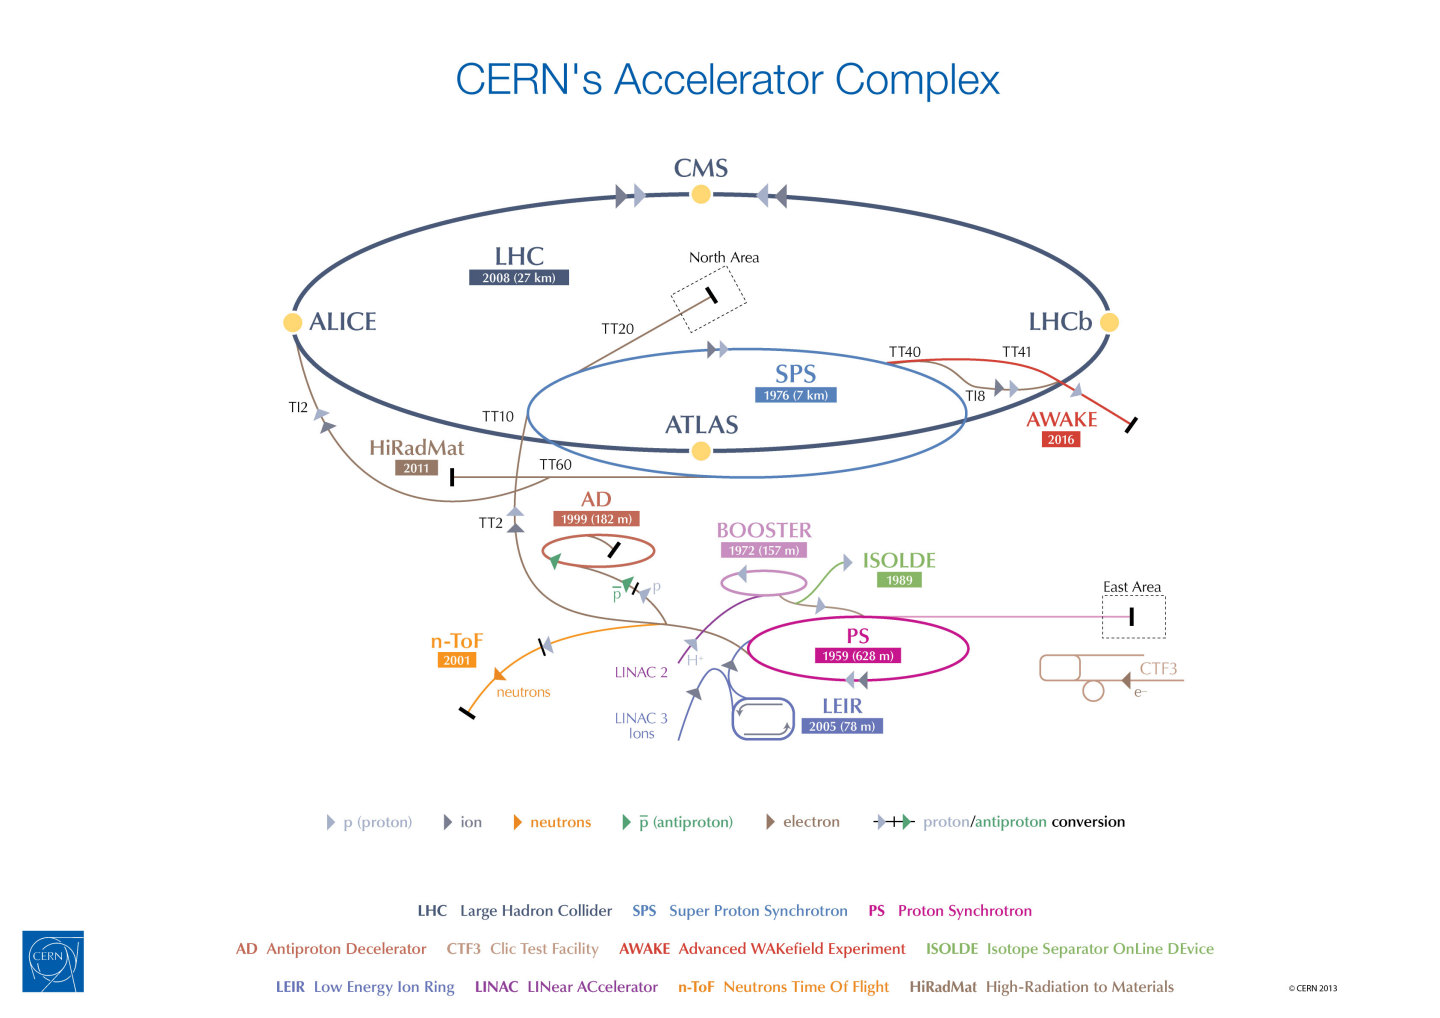
\includegraphics[scale=0.4]{CERN's-accelerator-complex2013.jpg}
\caption{The accelerator complex at CERN~\cite{Marcastel:1621583}.}
\label{fig:CERN_accelerator_complex}
\end{center}
\end{figure}

The protons are extracted by ionization from a hydrogen source and are accelerated to 50~{\MeV} by the linear accelerator LINAC2.
Then they are injected into the Proton Synchrotron Booster (PSB) where the proton energies are increased to 1.4~{\GeV} before they enter the Proton Synchrotron (PS) which accelerates the protons to 25~{\GeV}.
Next, the proton energies are increasing to 450~{\GeV} in the Super Proton Synchrotron (SPS). 
Finally, the protons are split into two beams and enter the LHC where the two beams run in two adjacent beam pipes with opposite directions.
In order to keep the protons on the circular trajectory in the LHC, 1232 superconducting dipole magnets~\cite{1288863} generate a magnetic field strength of 8.33~T to bend the proton beams in eight arcs.
Additionally, 392 quadrupole magnets~\cite{1288863} are installed to focus the beam.
A cryogenic system running with super-fluid helium-4 is used to cool down the superconducting magnets to a temperature of 1.7~K.

For a given physics process, the event rate is proportional to the cross section $\sigma$ of this process.
\begin{equation}
\frac{dN}{dt} = \mathcal{L}\cdot\sigma
\end{equation}
where $N$ is the number of events and $\mathcal{L}$ denotes the luminosity of the beam.
The luminosity of the beam, $\mathcal{L}$ can be calculated by
\begin{equation}
\mathcal{L} = \frac{N^{2} f}{4 \pi \sigma_{x} \sigma_{y}} \cdot F
\end{equation}
where $N$ is the number of protons, $f$ is the bunches crossing frequency, and the $\sigma_{x}$ and $\sigma_{y}$ are the $x$ and $y$ components for cross section $\sigma$.
The geometric luminosity reduction factor, $F$, is related to the crossing angle at the Interaction Point (IP).
Considering a beam consisting of $1.15 \times 10^{11}$ protons with bunching spacing of 25~ns, the transversal size of the bunch at Interaction Pointe $16\times 10^{-4}$~cm, and taking the geometric luminosity reduction factor as 1, the design luminosity of $10^{34}$~cm$^{-2}$s$^{-1}$ can be reached.

The first beam was circulated through the collider on the morning of 10 September 2008~\cite{CERN-COURIER-Sep192008}.
However, a magnet quench incident occurred on 19 September 2008 and caused extensive damage to over 50 superconducting magnets, their mountings, and the vacuum pipe.
Most of 2009 was spent on repairs the damage caused by the magnet quench incident and the operations resumed on 20 November of that year.
The first phase of data-taking (Run 1) started at the end of 2009 and the beam energy was increased to a centre-of-mass $\sqrt{s}=7$~{\TeV} in 2011 and $\sqrt{s} = 8$~{\TeV} in 2012.
The total integrated luminosity of 5.46~{\ifb} was collected in 2011 and of 22.8~{\ifb} was collected in 2012.
Since 13 February 2013 the LHC was in the Long Shutdown 1 (LS1) phase for maintenance and upgrades.
On 5 April 2015, the LHC restarted and was operating at a centre-of-mass energy $\sqrt{s}=13$~{\TeV} throughout the Run 2 phase\footnote{The Run 2 data-taking started from 2015}.


%%%%%
%%%%%
%%%%%

\section{The ATLAS experiment}

The ATLAS\footnote{A Toroidal LHC Apparatus} detector~\cite{1748-0221-3-08-S08003} is a multi-purpose detector housed in its cavern at point 1 at the LHC~\cite{1748-0221-3-08-S08001}.
It is the largest experiment at the LHC with a length of 44~m, a diameter of 25~m, and a weight of approximately 7000 tonnes.
It consists of three high precision sub-detector systems which are arranged concentrically around the interaction point and in forward and backward symmetrically.
Related to this symmetry, the ATLAS detector is sectioned into the central barrel region with one end-cap region perpendicular to the beam pipe on either side.
Figure~\ref{fig:ATLAS_detector} shows an overview of the ATLAS detector with its major components.

\begin{figure}[htbp]
\begin{center}
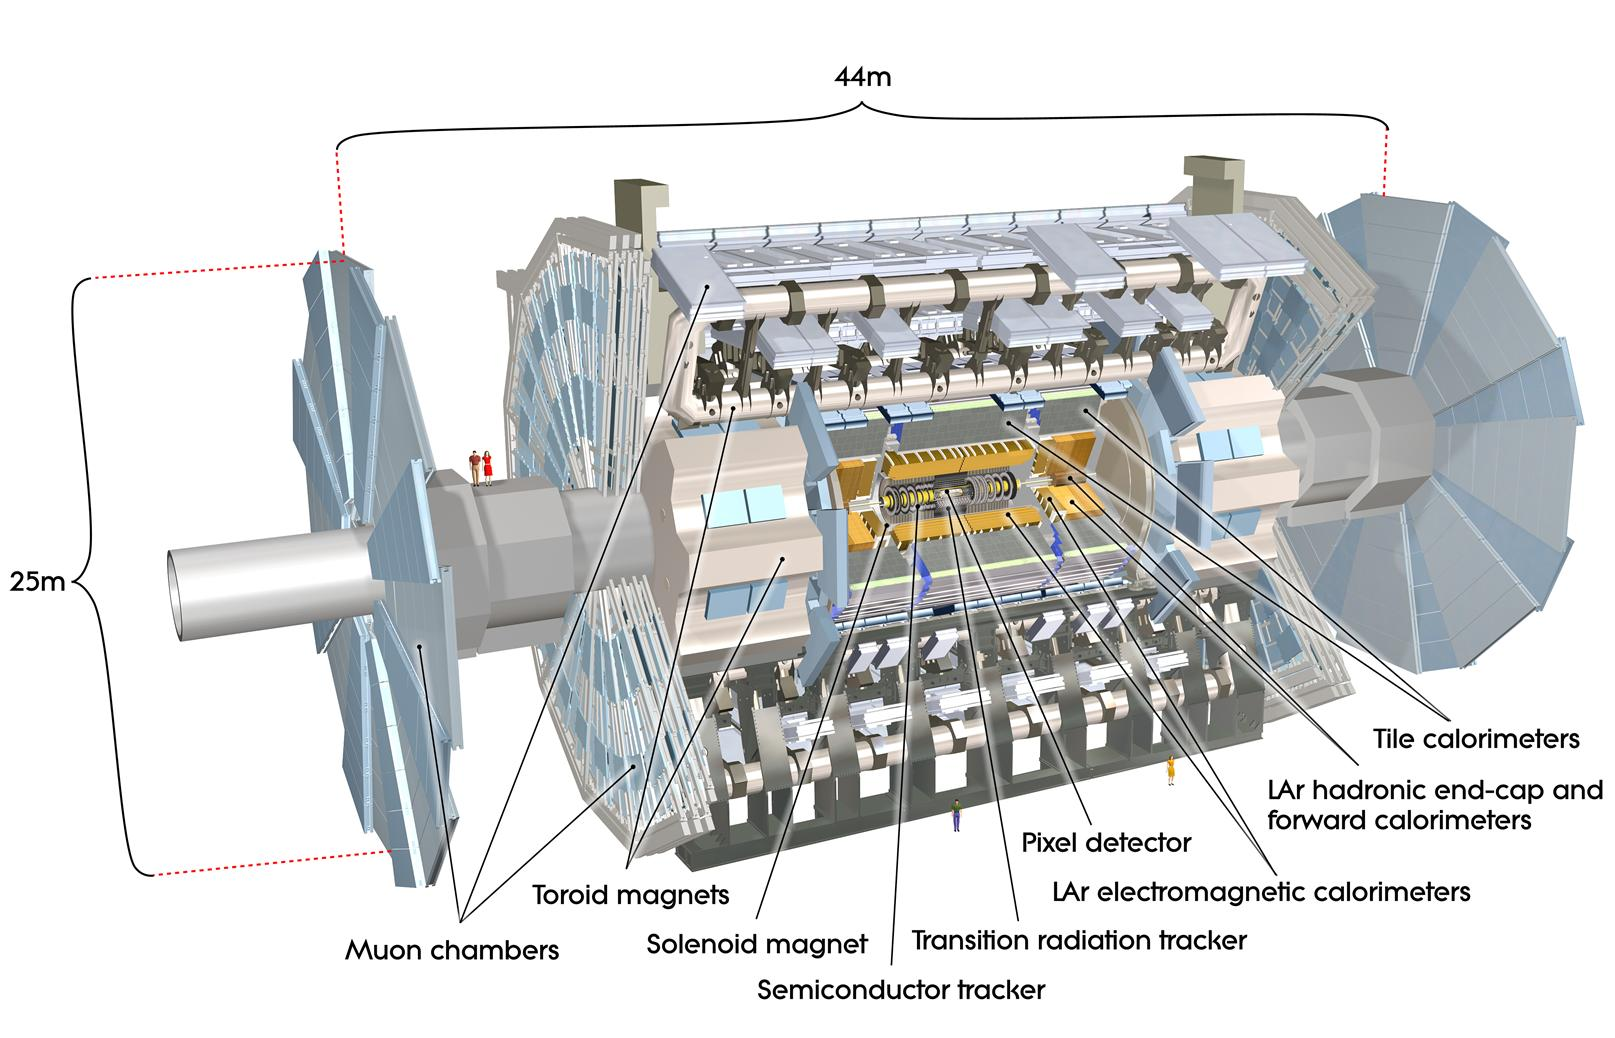
\includegraphics[scale=0.5]{0803012_01-A4-at-144-dpi.jpg}
\caption{Overview of the ATLAS detector~\cite{1748-0221-3-08-S08003}.}
\label{fig:ATLAS_detector}
\end{center}
\end{figure}

The ATLAS detector is designed to record the proton-proton interactions delivered by the LHC.
It can identify particles and measure their tracks and energies with very high precision, therefore, it is sensitive to large areas of particle physics phenomena from the precision measurement of the Standard Model (SM) to beyond the SM.
The detector is constituted by three sub-detector systems and the magnet system.
The innermost part of the detector is called the inner detector which identifies and reconstructs the charged particles as well as the primary and secondary vertices.
Around it, the calorimeter system is built as a cylindrical barrel with caps at each end to measure the particle energies.
The detector is completed by the muon spectrometer which performs identification and measurement of momenta of muons.
The magnetic system produces a field of $B$ = 0.5~T and $B$ = 1~T at barrel and two end-cap, respectively.
The detector has to withstand large collision rates with approximately 1000 particles per collision, therefore, a fast readout and a three-level trigger system are implemented to reduce the event rate from 40~MHz to 200~Hz.
The ATLAS coordinate system and the detail of each sub-detector systems are described in the following sections.

\subsection{The ATLAS coordinate system}

ATLAS uses a right-handed coordinate system with its origin at the nominal proton-proton interaction point (IP) in the centre of the detector and the $z$-axis along the beam pipe.
Along the $z$-axis the detector is divided into side-A (positive $z$) and side-C (negative $z$).
The positive $x$-axis is defined by the direction pointing from the IP to the centre of the LHC ring, and the positive $y$-axis points upward.%Cylindrical coordinates $(r, \phi)$ are used in the transverse plane.
The azimuthal angle $\phi$ is measured around the beam pipe  and the polar angle $\theta$ is the angle from the $z$-axis.
The transverse momentum $p_{\mathrm{T}}$, the transverse energy $E_{\mathrm{T}}$ and the missing transverse
energy $E_{\mathrm{T}}^{\mathrm{miss}}$ are defined in the transverse plane\footnote{$x-y$ plane}, here exemplary for $p_{\mathrm{T}}$:
%
\begin{equation}
p_{\mathrm{T}}= \sqrt{p_{x}^{2} + p_{y}^{2}}
\end{equation}
%
An important quantity in hadron collider physics is the \textbf{rapidity}, $y$, because of the invariance $y$ under Lorentz boosts in the longitudinal direction.
The rapidity is defined as
%
\begin{equation}
y = \frac{1}{2} \ln\Big[\frac{E + p_{z}}{E - p_{z}}\Big]
\end{equation}
%
where $E$ denotes the particle energy and $p_{z}$  is the component of the momentum along the beam direction.
Since mainly leptons can be considered massless in respect to the nominal centre-of-mass energy, the pseudorapidity, $\eta$, is used in stead of using the $y$.
For a massless particle, the \textbf{pseudorapidity}, $\eta$, depends on the polar angle $\theta$ through:
%
\begin{equation}
\eta = - \ln \tan \frac{\theta}{2}
\end{equation}
%
For a particle with the energy $E$ much larger than its mass, the approximation $E \approx |\vec{p}|$ is valid.
The distance, $\Delta R$, between two objects in the $\eta-\phi$ plan is given by
%
\begin{equation}
\Delta R = \sqrt{\Delta \eta^{2} + \Delta \phi^{2}}
\end{equation}
%
where $\Delta \eta$ and $\Delta \phi$ are the difference in pseudorapidity and azimuthal angle, respectively.

\subsection{The Inner Detector and Tracking System}
\label{subsec:inner_detector}

The Inner Detector (ID) consists of three sub-detectors: the Pixel detector, the silicon microstrip trackers  (SCT), and the Transition Radiation Tracker (TRT).
The main purpose of the ID is to provide high precision measurements of the tracks of particles and to reconstruct the primary and secondary vertices.
Each sub-detectors are composed of several layers of material which interacts with the charged particles when the charged particles penetrate the layers.
A  2~T magnetic field generated by the central solenoid parallel to the beam axis is applied to bend the charged particles using the Lorentz force.
By using the radius $r$ of the curvature of the tracks, the magnetic field strength $B$, and the charge of the particle $q$, we can calculate the magnitude of the transverse momentum \pt:
\begin{equation}
\pt = |q|Br
\end{equation}
The layout of the ID is illustrated in Figure~\ref{fig:Inner_detector} and the detail of sub-detectors are described in the following paragraphs.

\begin{figure}[htbp]
\begin{center}
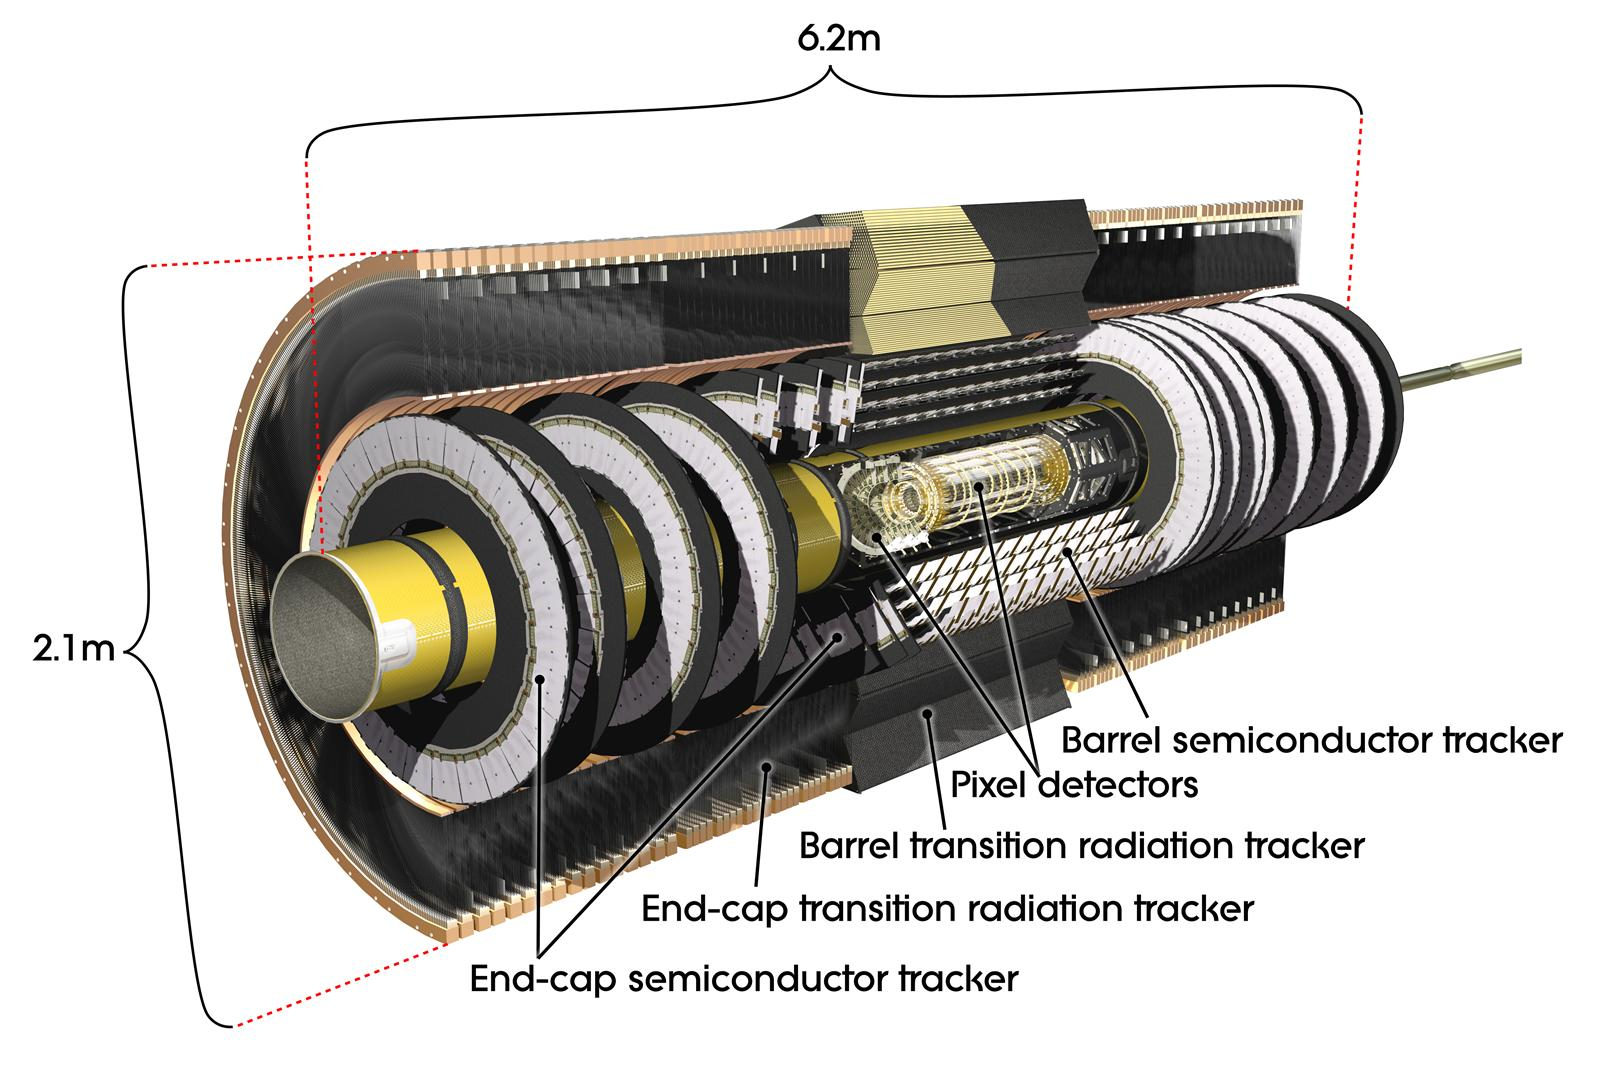
\includegraphics[scale=0.5]{0803014_01-A4-at-144-dpi.jpg}
\caption{Cut-away view of the ATLAS inner detector~\cite{1748-0221-3-08-S08003}.}
\label{fig:Inner_detector}
\end{center}
\end{figure}

%\subsubsection{Pixel Detector}
\noindent \textbf{Pixel Detector}

The innermost part of the entire ATLAS detector components is the Pixel detector which is composed of three barrel layers and three end-cap disks on each side.
The three cylindrical barrel layers around the beam axis have radial positions of 50.5~mm, 88.5~mm, and 122.5~mm respectively and they are made of 22, 38, and 52 identical staves respectively.
Each stave is inclined with azimuthal angle of 20 degrees and is composed of 13 pixel modules with 46,080 readout channel per module.
The size of each pixel is $50 \times 400~\mu m^{2}$ in $R-\phi \times z$.
In the forward region, three disks on each side equip the modules identical to the barrel modules, except the connecting cables. 
The total 1,744 modules in the pixel detector lead to nearly 80 million channel readout and provide the intrinsic accuracies of $10~\mu m$ in $R-\phi$ plane and $115~\mu m$ in $z$ direction covering the region $|\eta| < 2.5$. 

%\subsubsection{Semi Conductor Tracker}
\noindent \textbf{Semi Conductor Tracker}

On the top of the pixel detector is the Semi Conductor Tracker (SCT) which is a silicon strip detector.
There are about 6.3 million readout channels which are arranged in 4088 microstrips.
The intrinsic accuracies per sensor is $17~\mu m$ in $R-\phi$ and $580~\mu m$ in $z$ direction for the barrel and in $R$ for the  disks, respectively.
Similar to the pixel detector, the SCT covers the region $|\eta| < 2.5$ and consists of 8 strip layers in barrel and a total of 9 discs in the end-cap region on each side.
No track reconstruction is possible beyond the covered pseudorapidity range.
Therefore, the electrons cannot be distinguished from photons above $|\eta| > 2.5$ region.

%\subsubsection{Transition Radiation Tracker}
\noindent \textbf{Transition Radiation Tracker}

The outermost component of the ID is the Transition Radiation Tracker (TRT) which consists of 4~mm diameter straw tubes filled with the xenon-based gas mixture.
The gas mixture are ionized by charged particles when they penetrates the straws.
The ionized electrons drift to the cathode because a high voltage is applied on the tungsten wire in the center of the straw tube.
Therefore, the TRT allows the enhanced electron identification, momentum measurement, vertex measurement.
In the barrel region, the straws are surrounded by polypropylene fibres and are divided into two halves at $|\eta|=0$.
In the end-caps, the straws are arranged radially and surrounded by foils as a transition radiation element.
They are read out at two sides and at the center of the TRT with the total number of the readout channels of TRT are approximately 350,000.
The TRT only provides information in the $R-\phi$ plane with an intrinsic accuracy of 130~$\mu$m per straw and covers a range up to $|\eta| < 2.0$. 

%\subsubsection{Solenoid Magnet}
\noindent \textbf{Solenoid Magnet}

A superconducting solenoid magnet encloses the ID and produces a 2~T magnetic field to bend the trajectories of the charged particles.
A cooling system is used and shared with the electromagnetic calorimeter~\ref{subsec:calorimeter} to reduced the deterioration of the energy measurement.

\subsection{The Calorimeters}
\label{subsec:calorimeter}

The calorimeters are used to measure the energy of particles, such as electrons, photons, and jets.
Besides muons, all electromagnetically or haronically interacting particles are stopped in the calorimeters by absorbing their energy.
Not only charged particles but also neutral particles such as photons and neutral hadrons can be detected in the calorimeter.
By requiring highly hermiticity of the calorimeter, the missing energy can be reconstructed precisely as negative vectorial sum of all energy deposits.
The ATLAS Calorimeters system are placed between the Inner Detector~\ref{subsec:inner_detector} and the Muon Spectrometer~\ref{subsec:the_muon_spectrometer}.
The ATLAS calorimeters system consist of an inner Electromagnetic and outer Hadronic Calorimeter together with the Forward Calorimeter.
The Electromagnetic Calorimeter is dedicated for measuring electrons and photons, and the Hadronic Calorimeter focusing on hadronically interacting particles.
The calorimeters cover a range $|\eta| < 4.9$.
An layout view of the ATLAS Calorimeters system is shown in Figure~\ref{fig:calorimeter}

%\subsubsection{Electromagnetic Calorimeter}
\noindent \textbf{Electromagnetic Calorimeter}

The Electromagnetic Calorimeters (ECAL) measure the energy of electrons and photons as they interact with matter.
The ECAL consists of layers of high-density material, lead, as absorbers and interleaved with layers of liquid argon (LAr) as active medium.





%\subsubsection{Hadronic Calorimeter}
\noindent \textbf{Hadronic Calorimeter}


Hadrons, which are signi cantly heavier and mainly interact via the strong force, propagate further causing more wide-spread hadronic showers mainly in the denser Hadronic Calorimeter.

%\subsubsection{Forward Calorimeter}
\noindent \textbf{Forward Calorimeter}


\begin{figure}[htbp]
\begin{center}
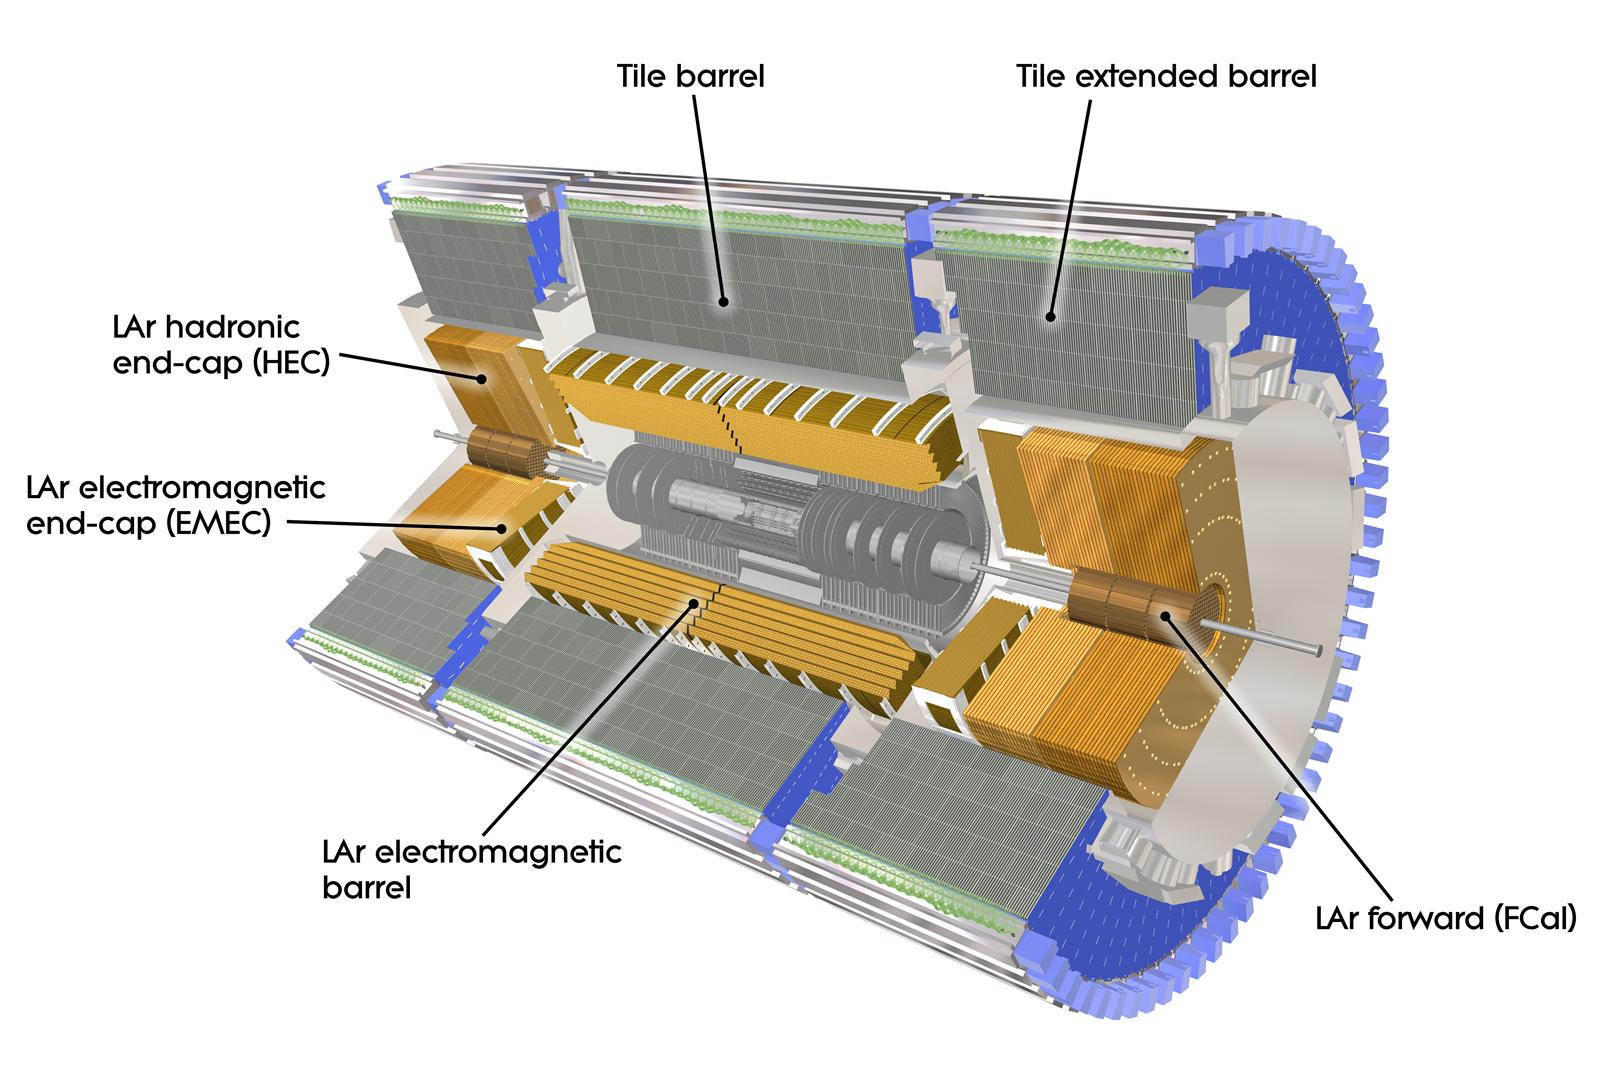
\includegraphics[scale=0.5]{0803015_01-A4-at-144-dpi.jpg}
\caption{Cut-away view of the calorimeter system~\cite{1748-0221-3-08-S08003}.}
\label{fig:calorimeter}
\end{center}
\end{figure}

\begin{table}[htbp]
\begin{center}
\begin{tabular}{cc}
\hline
\hline
Calorimeter & Required resolution\\
\hline
ElectromagneticCalorimeter & $\sigma_{E}/E = 10\% / \sqrt{E\mathrm{ (GeV)}} \oplus 0.7\%$\\
Hadronic Calorimeter & $\sigma_{E}/E = 50\% / \sqrt{E~\mathrm{(GeV)}} \oplus 3\%$\\
Forward Calorimeter & $\sigma_{E}/E = 100\% / \sqrt{E~\mathrm{(GeV)}} \oplus 10\%$\\
\hline
\hline
\end{tabular}
\end{center}
\caption{Resolution requirements for the different calorimeters of the ATLAS detector~\cite{1748-0221-3-08-S08003}.}
\label{tab:}
\end{table}%







\subsection{The Muon Spectrometer} \label{subsec:the_muon_spectrometer}

The outermost part of the ATLAS detector is the Muon Spectrometer~\cite{1748-0221-3-08-S08003}~\cite{Palestini:681459}~\cite{0910.2767}.
Muons have the same properties as electrons but 200 times heavier than the electrons and muons don't interact predominately by Bremsstrahlung but have minimal ionizing at LHC energy in the inner layers of the detector.
Only the muons with an energy less than 5~{\GeV} are stopped before the Muon Spectrometer.
Therefore, muons are the only measurable particles that can penetrate the Inner Detector and the Calorimeters.
In order to determine the muon momentum with high precision, a detector that concentrates on the measurement of muons is necessary.

The Muon Spectrometer is designed to measure the transverse momentum ($p_{\mathrm{T}}$) of muons with $p_{\mathrm{T}} > 3$~{\GeV} with a resolution of 3\% for $p_{\mathrm{T}} < 250$~{\GeV} and increasing to 10\% at 1~{\TeV}.
It consists of large toroid magnets system and three layers of high precision tracking chambers which allow a precise measurement of the muon momentum over nearly the full solid angle.
The barrel toroid magnet system is composed of eight superconducting coils which are installed radial symmetrically around the beam pipe.
It covers the range $|\eta| < 1.4$ and bends the trajectories of muons with the bending power 1.5 to 5.5 Tm.
The magnetic field produced by the barrel toroid magnets provides an approximately 1~T field at the center of each coils, but is rather non-uniform, especially in the barrel-endcap transition region.
In the endcap toroid magnets system, the magnetic field is provided by eight superconducting coils, closed in an insulation vessel extending to about 10 m in diameter, located between the first and the second station of tracking chambers.
The endcap toroid magnets cover $1.6 < |\eta| < 2.4$ and provide a a magnetic field in the range of 1 to 2 T with bending power 1 to 7.5 Tm.

The Monitored Drift Tubes (MDTs) consists of cylindrical drift tubes, filled with a gas mixture of argon and carbon dioxide.
A tungsten-rhenium alloyed aluminium wire in the centre of each tube collects the electrons freed by ionization of the gas volume by traversing muons.
The MDTs covers a full range of $|\eta| < 2.7$, while the inner layer only covers $|\eta| < 2.0$.
The Cathode Strip Chambers (CSCs) provides a coverage range $2.0 < |\eta| < 2.7$, where MDTs would have occupancy problems.
Both MDTs and CSCs are used for precision tracking in the spectrometer bending plane and end-cap inner layer, respectively.
The Resistive Plate Chambers (RPCs) and Thin Gap Chambers (TGCs) are used for triggering in barrel and end-cap, they have sufficient intrinsic time resolution of 1.5 ns and 4 ns, respectively.
A sketch of the Muon Spectrometer and its four components are depicted in Figure~\ref{fig:muon_spectrometer} and Table~\ref{tab:muon_spectrometer_components} gives a summary of the Muon Spectrometer components

\begin{figure}[htbp]
\begin{center}
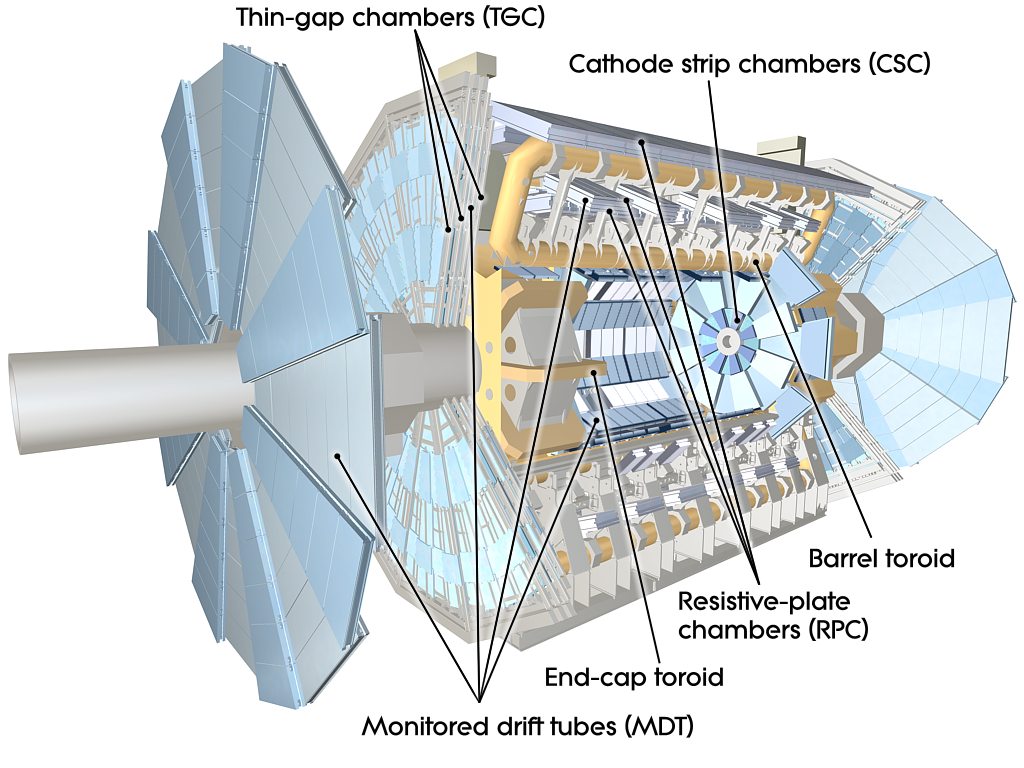
\includegraphics[scale=0.4]{MuonSystem_d3.png}
\caption{Sketch of the muon system of the ATLAS detector~\cite{1748-0221-3-08-S08003}.}
\label{fig:muon_spectrometer}
\end{center}
\end{figure}

\begin{table}[htbp]
\begin{center}
\begin{tabular}{ccccc}
\hline
\hline
Type & Purpose & Location & $\eta$ coverage & Channel\\
\hline
MDT & Tracking & barrel + end-cap & $0.0 < \eta < 2.7$ & 354k\\
CSC & Tracking & end-cap layer 1 & $2.0 < \eta < 2.7$ & 30.7k\\
RPC & Trigger & barrel & $0.0 < \eta < 1.0$ & 373k\\
TGC & Trigger & end-cap & $1.0 < \eta < 2.4$ & 318k\\
\hline
\hline
\end{tabular}
\end{center}
\caption{A summary of the Muon Spectrometer components.}
\label{tab:muon_spectrometer_components}
\end{table}%

\subsection{The Trigger System and Data Acquisition}

\subsection{}



%\chapter{}
%\label{chapter:}
%\graphicspath{{figures/}
%\input{chapter_}

%\chapter{}
%\label{chapter:}
%\graphicspath{{figures/}
%\input{chapter_}

%\chapter{}
%\label{chapter:}
%\graphicspath{{figures/}
%\input{chapter_}

%\FloatBarrier

%\chapter{}
%\label{chapter:}
%\graphicspath{{figures/}
%\input{chapter_}

%------------------------------------------------------------------------------- 
\clearpage

\appendix
\part*{Appendix}
\addcontentsline{toc}{part}{Appendix}

\chapter{Simulated samples}
\label{app:samples}
%\graphicspath{figures/samples/}
The Monte Carlo (MC) samples are used to model the SUSY signals and to estimate the SM background.
The MC samples are processed using a ATLAS detector full simulation (FullSim) or a fast simulation (AFII\footnote{AFII stands for ATLAS Fast II.}) based on {\GEANT}4~\cite{Agostinelli:2002hh} simulation package.
The FullSim simulates the detailed properties of the ATLAS detector while the AFII uses a parameterized calorimeter response and simulates ID and MS~\cite{ATLAS:1300517} based on {\GEANT}4.
The simulated MC events are reweighted to the observed pile-up conditions in the data.

%%%
%%%
%%%

\section{Samples used for strong interaction}
\label{sec:app_samples_strong}

Table~\ref{tab:app_sample_strong} shows the event generator, parton shower, cross-section normalization, PDF set~\cite{Martin:2009iq}, and the set of tunned parameters for modelling for all samples.
Except those produced by the {\SHERPA}, the \textsc{EvtGEN}\xspace v1.2.0 package~\cite{Lange:2001uf} is used to model the properties of bottom and charm hadron decays for all MC samples.

\begin{table}[htp]
%\begin{center}
\resizebox{\textwidth}{!}{% <------ Don't forget this %
\begin{tabular}{ccccccc}
\hline
\hline
Signal/Background                                      & Physics process                   & Event generator                  & Parton shower     & Cross-section normalization & PDF set    & Set of tunned parameters\\
\hline
\hline
\multirow{3}{*}{Signal}                                & RPC                               & MG5\_{\scriptsize A}MC@NLO 2.2.3 & {\PYTHIA} 8.186   & NLO+NLL                     & NNPDF2.3LO & A14\\
                                                       & RPV (except Figure~\ref{})        & MG5\_{\scriptsize A}MC@NLO 2.2.3 & {\PYTHIA} 8.210   & or                          & NNPDF2.3LO & A14\\
                                                       & RPV (Figure~\ref{})               & {\HERWIGpp} 2.7.1                & {\HERWIGpp} 2.7.1 & NLO-Prospino2               & CTEQ6L1    & UEEE5\\
\hline
\multirow{3}{*}{\shortstack{$t\bar{t}+X$\\background}} & $t\bar{t}W, t\bar{t}Z/\gamma^{*}$ & MG5\_{\scriptsize A}MC@NLO 2.2.2 & {\PYTHIA} 8.186   & NLO                         & NNPDF2.3LO & A14\\
                                                       & $t\bar{t}H$                       & MG5\_{\scriptsize A}MC@NLO 2.3.2 & {\PYTHIA} 8.186   & NLO                         & NNPDF2.3LO & A14\\
                                                       & 4$t$                              & MG5\_{\scriptsize A}MC@NLO 2.2.2 & {\PYTHIA} 8.186   & NLO                         & NNPDF2.3LO & A14\\
\hline
\multirow{2}{*}{\shortstack{Dibosno\\background}}      & $ZZ, WZ$                          & {\SHERPA} 2.2.1                  & {\SHERPA} 2.2.1   & NLO                         & NNPDF2.3LO & {\SHERPA} default\\
                                                       & Other (inc. $W^{\pm}W^{\pm}$)     & {\SHERPA} 2.1.1                  & {\SHERPA} 2.1.1   & NLO                         & CT10       & {\SHERPA} default\\
\hline
\multirow{4}{*}{\shortstack{Rare\\background}}         & $t\bar{t}WW, t\bar{t}WZ$          & MG5\_{\scriptsize A}MC@NLO 2.2.2 & {\PYTHIA} 8.186   & NLO                         & NNPDF2.3LO & A14\\
                                                       & $tZ, tWZ, tt\bar{t}$              & MG5\_{\scriptsize A}MC@NLO 2.2.2 & {\PYTHIA} 8.186   & LO                          & NNPDF2.3LO & A14\\
                                                       & $WH, ZH$                          & MG5\_{\scriptsize A}MC@NLO 2.2.2 & {\PYTHIA} 8.186   & NLO                         & NNPDF2.3LO & A14\\
                                                       & Triboson                          & {\SHERPA} 2.1.1                  & {\SHERPA} 2.1.1   & NLO                         & CT10       & {\SHERPA} default\\
\hline
\hline
\end{tabular}
%\end{center}
}
\caption{The simulated signal and background MC samples.
The event generator, parton shower, cross-section normalization, PDF set, and the set of tunned parameters for each samples are shown.
The $t\bar{t}WW, t\bar{t}WZ, tZ, tWZ, tt\bar{t}, WH, ZH$ and triboson background samples are labeled in the "rare" because they contribute a very small amount to the signal region.}
\label{tab:app_sample_strong}
\end{table}%


%%%
%%%
%%%

\section{Samples used for weak interaction}
\label{sec:app_samples}

%%%
%%%
%%%

\chapter{Cross-sections of NUHM2}
\label{app:cross_sections}
%\graphicspath{figures/samples/}
 The cross-sections, branching fraction, and filter efficiency for the NUHM2 signal samples are shown in Table~\ref{tab:app_xsec_m12_300}, \ref{tab:app_xsec_m12_350}, \ref{tab:app_xsec_m12_400}, \ref{tab:app_xsec_m12_500}, \ref{tab:app_xsec_m12_600}, \ref{tab:app_xsec_m12_700} and \ref{tab:app_xsec_m12_800}.
 The various final states are listed in Table~\ref{tab:app_xsec_final_state}

\begin{table}[htp]
%\begin{center}
\resizebox{\textwidth}{!}{% <------ Don't forget this %
{\tiny
\begin{tabular}{cccccc}
\hline
\hline
DSID   & Final state & Cross-section [$pb$] & K-factor/BF  & Filter efficiency & Relative uncertainty\\
\hline
370617 & 111         & 0.0116116904         & 1.00000000   & 1.00000000        & 0.07950234\\
370617 & 112         & 0.0009775530         & 1.00000000   & 1.00000000        & 0.08535312\\
370617 & 113         & 0.5163867234         & 1.00000000   & 1.00000000        & 0.07315089\\
370617 & 114         & 0.0000593483         & 1.00000000   & 1.00000000        & 0.08483826\\
370617 & 115         & 1.1555478731         & 1.00000000   & 1.00000000        & 0.06803190\\
370617 & 116         & 0.0056717958         & 1.00000000   & 1.00000000        & 0.05803524\\
370617 & 117         & 0.7027932124         & 1.00000000   & 1.00000000        & 0.08979719\\
370617 & 118         & 0.0030806972         & 1.00000000   & 1.00000000        & 0.07709474\\
370617 & 122         & 0.0000260248         & 1.00000000   & 1.00000000        & 0.13101757\\
370617 & 123         & 0.1709342503         & 1.00000000   & 1.00000000        & 0.06993300\\
370617 & 124         & 0.0002175469         & 1.00000000   & 1.00000000        & 0.08148442\\
370617 & 125         & 0.4768609298         & 1.00000000   & 1.00000000        & 0.06541649\\
370617 & 126         & 0.0228714654         & 1.00000000   & 1.00000000        & 0.05697991\\
370617 & 127         & 0.2784795051         & 1.00000000   & 1.00000000        & 0.08434059\\
370617 & 128         & 0.0120807622         & 1.00000000   & 1.00000000        & 0.07942795\\
370617 & 133         & 0.0003583977         & 1.00000000   & 1.00000000        & 0.06910802\\
370617 & 134         & 0.0191236271         & 1.00000000   & 1.00000000        & 0.06575101\\
370617 & 135         & 0.6773400626         & 1.00000000   & 1.00000000        & 0.06477621\\
370617 & 136         & 0.0262277631         & 1.00000000   & 1.00000000        & 0.05716003\\
370617 & 137         & 0.3954923581         & 1.00000000   & 1.00000000        & 0.08483868\\
370617 & 138         & 0.0137758494         & 1.00000000   & 1.00000000        & 0.08211888\\
370617 & 144         & 0.0000568127         & 1.00000000   & 1.00000000        & 0.07453184\\
370617 & 145         & 0.0213534960         & 1.00000000   & 1.00000000        & 0.05398319\\
370617 & 146         & 0.2119219378         & 1.00000000   & 1.00000000        & 0.05665419\\
370617 & 147         & 0.0113003976         & 1.00000000   & 1.00000000        & 0.07780129\\
370617 & 148         & 0.1028839844         & 1.00000000   & 1.00000000        & 0.07544194\\
370617 & 157         & 1.1640104660         & 1.00000000   & 1.00000000        & 0.07733674\\
370617 & 158         & 0.0187939524         & 1.00000000   & 1.00000000        & 0.06417211\\
370617 & 167         & 0.0188413722         & 1.00000000   & 1.00000000        & 0.06767782\\
370617 & 168         & 0.1655520687         & 1.00000000   & 1.00000000        & 0.06249944\\
% Compressed, Higgsino LSP EWK analysis
394301 & 157         & 1.1640104660         & 0.1110699593 & 1.4334E-01        & 0.07733674\\
394302 & 127         & 0.2784795051         & 0.0365485123 & 2.5440E-01        & 0.08434059\\
394303 & 125         & 0.4768609298         & 0.0365485123 & 2.5135E-01        & 0.06541649\\
394304 & 112         & 0.0009775530         & 0.0365485123 & 3.0251E-01        & 0.08535312\\
\hline
\hline
\end{tabular}
%\end{center}
}
}
\caption{The cross-sections, branching fraction, and filter efficiency for the NUHM2 signal samples $m_{1/2} = 300$~{\GeV}.}
\label{tab:app_xsec_m12_300}
\end{table}%

\begin{table}[htp]
%\begin{center}
\resizebox{\textwidth}{!}{% <------ Don't forget this %
{\tiny
\begin{tabular}{cccccc}
\hline
\hline
DSID   & Final state & Cross-section [$pb$] & K-factor/BF & Filter efficiency & Relative uncertainty\\
\hline
370618 & 111         & 0.0076283799         & 1.00000000  & 1.00000000        & 0.07739107\\
370618 & 112         & 0.5835187445         & 1.00000000  & 1.00000000        & 0.07193879\\
370618 & 113         & 0.0000894312         & 1.00000000  & 1.00000000        & 0.09912250\\
370618 & 114         & 0.0001023491         & 1.00000000  & 1.00000000        & 0.07825966\\
370618 & 115         & 1.0850849571         & 1.00000000  & 1.00000000        & 0.07591545\\
370618 & 116         & 0.0049251988         & 1.00000000  & 1.00000000        & 0.05689268\\
370618 & 117         & 0.6538672654         & 1.00000000  & 1.00000000        & 0.08886870\\
370618 & 118         & 0.0025928251         & 1.00000000  & 1.00000000        & 0.07604635\\
370618 & 122         & 0.0003076705         & 1.00000000  & 1.00000000        & 0.06756051\\
370618 & 123         & 0.1082826561         & 1.00000000  & 1.00000000        & 0.06926016\\
370618 & 124         & 0.0094622361         & 1.00000000  & 1.00000000        & 0.06300188\\
370618 & 125         & 0.6833463531         & 1.00000000  & 1.00000000        & 0.06443308\\
370618 & 126         & 0.0129259483         & 1.00000000  & 1.00000000        & 0.05402434\\
370618 & 127         & 0.3983657446         & 1.00000000  & 1.00000000        & 0.08599203\\
370618 & 128         & 0.0066391822         & 1.00000000  & 1.00000000        & 0.07534667\\
370618 & 133         & 0.0000649975         & 1.00000000  & 1.00000000        & 0.10705877\\
370618 & 134         & 0.0001247362         & 1.00000000  & 1.00000000        & 0.07583934\\
370618 & 135         & 0.2353276570         & 1.00000000  & 1.00000000        & 0.06552596\\
370618 & 136         & 0.0091529911         & 1.00000000  & 1.00000000        & 0.05672728\\
370618 & 137         & 0.1357101599         & 1.00000000  & 1.00000000        & 0.08410482\\
370618 & 138         & 0.0046580255         & 1.00000000  & 1.00000000        & 0.07466805\\
370618 & 144         & 0.0000282761         & 1.00000000  & 1.00000000        & 0.07380597\\
370618 & 145         & 0.0104731869         & 1.00000000  & 1.00000000        & 0.05738262\\
370618 & 146         & 0.1421425400         & 1.00000000  & 1.00000000        & 0.06087756\\
370618 & 147         & 0.0054325991         & 1.00000000  & 1.00000000        & 0.07452907\\
370618 & 148         & 0.0669626098         & 1.00000000  & 1.00000000        & 0.07470349\\
370618 & 157         & 0.9548695995         & 1.00000000  & 1.00000000        & 0.07280905\\
370618 & 158         & 0.0093028684         & 1.00000000  & 1.00000000        & 0.06338077\\
370618 & 167         & 0.0092973351         & 1.00000000  & 1.00000000        & 0.06299140\\
370618 & 168         & 0.1082938946         & 1.00000000  & 1.00000000        & 0.05684157\\
% Compressed, Higgsino LSP EWK analysis
394305 & 157         & 0.9548695995         & 0.111060393 & 1.2990E-01        & 0.07280905\\
394306 & 127         & 0.3983657446         & 0.101384714 & 2.5255E-01        & 0.08599203\\
394307 & 125         & 0.6833463531         & 0.101384714 & 2.5574E-01        & 0.06443308\\
394308 & 112         & 0.5835187445         & 0.101384714 & 2.2766E-01        & 0.07193879\\
\hline
\hline
\end{tabular}
%\end{center}
}
}
\caption{The cross-sections, branching fraction, and filter efficiency for the NUHM2 signal samples $m_{1/2} = 350$~{\GeV}.}
\label{tab:app_xsec_m12_350}
\end{table}%

\begin{table}[htp]
%\begin{center}
\resizebox{\textwidth}{!}{% <------ Don't forget this %
{\tiny
\begin{tabular}{cccccc}
\hline
\hline
DSID   & Final state & Cross-section [$pb$] & K-factor/BF & Filter efficiency & Relative uncertainty\\
\hline
370619 & 111         & 0.0050511346         & 1.00000000  & 1.00000000        & 0.07579917\\
370619 & 112         & 0.6255603991         & 1.00000000  & 1.00000000        & 0.07158509\\
370619 & 113         & 0.0000109243         & 1.00000000  & 1.00000000        & 0.09579487\\
370619 & 114         & 0.0001052946         & 1.00000000  & 1.00000000        & 0.07766307\\
370619 & 115         & 1.0342689914         & 1.00000000  & 1.00000000        & 0.06820123\\
370619 & 116         & 0.0035382215         & 1.00000000  & 1.00000000        & 0.05558890\\
370619 & 117         & 0.6163842668         & 1.00000000  & 1.00000000        & 0.08756721\\
370619 & 118         & 0.0018044868         & 1.00000000  & 1.00000000        & 0.07509790\\
370619 & 122         & 0.0002664650         & 1.00000000  & 1.00000000        & 0.07041738\\
370619 & 123         & 0.0628066056         & 1.00000000  & 1.00000000        & 0.06735393\\
370619 & 124         & 0.0048696810         & 1.00000000  & 1.00000000        & 0.06286865\\
370619 & 125         & 0.6845201512         & 1.00000000  & 1.00000000        & 0.06476776\\
370619 & 126         & 0.0067063042         & 1.00000000  & 1.00000000        & 0.05627793\\
370619 & 127         & 0.3976839861         & 1.00000000  & 1.00000000        & 0.08518583\\
370619 & 128         & 0.0033679821         & 1.00000000  & 1.00000000        & 0.07318125\\
370619 & 133         & 0.0000557211         & 1.00000000  & 1.00000000        & 0.10394707\\
370619 & 134         & 0.0000636446         & 1.00000000  & 1.00000000        & 0.07539568\\
370619 & 135         & 0.1183185424         & 1.00000000  & 1.00000000        & 0.05812791\\
370619 & 136         & 0.0036848994         & 1.00000000  & 1.00000000        & 0.05773533\\
370619 & 137         & 0.0670198462         & 1.00000000  & 1.00000000        & 0.08128406\\
370619 & 138         & 0.0018161476         & 1.00000000  & 1.00000000        & 0.07634830\\
370619 & 144         & 0.0000158930         & 1.00000000  & 1.00000000        & 0.07992644\\
370619 & 145         & 0.0054376416         & 1.00000000  & 1.00000000        & 0.05587952\\
370619 & 146         & 0.0976478188         & 1.00000000  & 1.00000000        & 0.06106615\\
370619 & 147         & 0.0027346724         & 1.00000000  & 1.00000000        & 0.07262348\\
370619 & 148         & 0.0442265190         & 1.00000000  & 1.00000000        & 0.07409153\\
370619 & 157         & 0.8415837349         & 1.00000000  & 1.00000000        & 0.07397928\\
370619 & 158         & 0.0047908009         & 1.00000000  & 1.00000000        & 0.06312184\\
370619 & 167         & 0.0047973169         & 1.00000000  & 1.00000000        & 0.06465433\\
370619 & 168         & 0.0724744359         & 1.00000000  & 1.00000000        & 0.06197995\\ 
% Compressed, Higgsino LSP EWK analysis
394309 & 157         & 0.8415837349         & 0.111047482 & 1.2199E-01        & 0.07397928\\
394310 & 127         & 0.3976839861         & 0.102934938 & 2.2044E-01        & 0.08518583\\
394311 & 125         & 0.6845201512         & 0.102934938 & 2.2387E-01        & 0.06476776\\
394312 & 112         & 0.6255603991         & 0.102934938 & 2.0415E-01        & 0.07158509\\
\hline
\hline
\end{tabular}
%\end{center}
}
}
\caption{The cross-sections, branching fraction, and filter efficiency for the NUHM2 signal samples $m_{1/2} = 400$~{\GeV}.}
\label{tab:app_xsec_m12_400}
\end{table}%

\begin{table}[htp]
%\begin{center}
\resizebox{\textwidth}{!}{% <------ Don't forget this %
{\tiny
\begin{tabular}{cccccc}
\hline
\hline
DSID   & Final state & Cross-section [$pb$] & K-factor/BF & Filter efficiency & Relative uncertainty\\
\hline
370620 & 111         & 0.0023867653         & 1.00000000  & 1.00000000        & 0.07209579\\
370620 & 112         & 0.6603094819         & 1.00000000  & 1.00000000        & 0.07005129\\
370620 & 113         & 0.0001325585         & 1.00000000  & 1.00000000        & 0.07482547\\
370620 & 114         & 0.0000688236         & 1.00000000  & 1.00000000        & 0.07197169\\
370620 & 115         & 0.9426500411         & 1.00000000  & 1.00000000        & 0.06460091\\
370620 & 116         & 0.0015013209         & 1.00000000  & 1.00000000        & 0.06183960\\
370620 & 117         & 0.5588686815         & 1.00000000  & 1.00000000        & 0.08560539\\
370620 & 118         & 0.0007279662         & 1.00000000  & 1.00000000        & 0.07490627\\
370620 & 122         & 0.0002061240         & 1.00000000  & 1.00000000        & 0.07176449\\
370620 & 123         & 0.0211437195         & 1.00000000  & 1.00000000        & 0.06388222\\
370620 & 124         & 0.0014907193         & 1.00000000  & 1.00000000        & 0.06151866\\
370620 & 125         & 0.6819165298         & 1.00000000  & 1.00000000        & 0.06356555\\
370620 & 126         & 0.0021061945         & 1.00000000  & 1.00000000        & 0.05664429\\
370620 & 127         & 0.3955900373         & 1.00000000  & 1.00000000        & 0.08416802\\
370620 & 128         & 0.0010081829         & 1.00000000  & 1.00000000        & 0.07123419\\
370620 & 133         & 0.0000195970         & 1.00000000  & 1.00000000        & 0.10671913\\
370620 & 134         & 0.0000176193         & 1.00000000  & 1.00000000        & 0.07871367\\
370620 & 135         & 0.0340389859         & 1.00000000  & 1.00000000        & 0.05924527\\
370620 & 136         & 0.0006926196         & 1.00000000  & 1.00000000        & 0.05800427\\
370620 & 137         & 0.0187411871         & 1.00000000  & 1.00000000        & 0.08099696\\
370620 & 138         & 0.0003229659         & 1.00000000  & 1.00000000        & 0.07606581\\
370620 & 144         & 0.0000098797         & 1.00000000  & 1.00000000        & 0.07455477\\
370620 & 145         & 0.0016797877         & 1.00000000  & 1.00000000        & 0.05654557\\
370620 & 146         & 0.0453186981         & 1.00000000  & 1.00000000        & 0.06092776\\
370620 & 147         & 0.0008077861         & 1.00000000  & 1.00000000        & 0.07385221\\
370620 & 148         & 0.0192295608         & 1.00000000  & 1.00000000        & 0.07792430\\
370620 & 157         & 0.7280789222         & 1.00000000  & 1.00000000        & 0.07328355\\
370620 & 158         & 0.0014642018         & 1.00000000  & 1.00000000        & 0.06676658\\
370620 & 167         & 0.0014587803         & 1.00000000  & 1.00000000        & 0.06499176\\
370620 & 168         & 0.0324683300         & 1.00000000  & 1.00000000        & 0.06503155\\
% Compressed, Higgsino LSP EWK analysis
394313 & 157         & 0.7280789222         & 0.111019377 & 1.0812E-01        & 0.07328355\\
394314 & 127         & 0.3955900373         & 0.105384522 & 1.8923E-01        & 0.08416802\\
394315 & 125         & 0.6819165298         & 0.105384522 & 1.8805E-01        & 0.06356555\\
394316 & 112         & 0.6603094819         & 0.105384522 & 1.7600E-01        & 0.07005129\\
\hline
\hline
\end{tabular}
%\end{center}
}
}
\caption{The cross-sections, branching fraction, and filter efficiency for the NUHM2 signal samples $m_{1/2} = 500$~{\GeV}.}
\label{tab:app_xsec_m12_500}
\end{table}%

\begin{table}[htp]
%\begin{center}
\resizebox{\textwidth}{!}{% <------ Don't forget this %
{\tiny
\begin{tabular}{cccccc}
\hline
\hline
DSID   & Final state & Cross-section [$pb$] & K-factor/BF & Filter efficiency & Relative uncertainty\\
\hline
370621 & 111         & 0.0012897690         & 1.00000000  & 1.00000000        & 0.07308455\\
370621 & 112         & 0.6656504736         & 1.00000000  & 1.00000000        & 0.07047924\\
370621 & 113         & 0.0001361496         & 1.00000000  & 1.00000000        & 0.07047382\\
370621 & 114         & 0.0000378018         & 1.00000000  & 1.00000000        & 0.07036880\\
370621 & 115         & 0.8824882181         & 1.00000000  & 1.00000000        & 0.06538492\\
370621 & 116         & 0.0006132703         & 1.00000000  & 1.00000000        & 0.05826096\\
370621 & 117         & 0.5187808653         & 1.00000000  & 1.00000000        & 0.08546879\\
370621 & 118         & 0.0002849360         & 1.00000000  & 1.00000000        & 0.07563404\\
370621 & 122         & 0.0001627043         & 1.00000000  & 1.00000000        & 0.06980768\\
370621 & 123         & 0.0078958339         & 1.00000000  & 1.00000000        & 0.06365983\\
370621 & 124         & 0.0005370949         & 1.00000000  & 1.00000000        & 0.06338450\\
370621 & 125         & 0.6791453722         & 1.00000000  & 1.00000000        & 0.06375124\\
370621 & 126         & 0.0007771667         & 1.00000000  & 1.00000000        & 0.05779085\\
370621 & 127         & 0.3930396433         & 1.00000000  & 1.00000000        & 0.08337329\\
370621 & 128         & 0.0003583832         & 1.00000000  & 1.00000000        & 0.07532675\\
370621 & 133         & 0.0000068529         & 1.00000000  & 1.00000000        & 0.09776310\\
370621 & 134         & 0.0000060514         & 1.00000000  & 1.00000000        & 0.07178228\\
370621 & 135         & 0.0118585454         & 1.00000000  & 1.00000000        & 0.06459092\\
370621 & 136         & 0.0001672449         & 1.00000000  & 1.00000000        & 0.05977911\\
370621 & 137         & 0.0063210120         & 1.00000000  & 1.00000000        & 0.07773831\\
370621 & 138         & 0.0000738669         & 1.00000000  & 1.00000000        & 0.07600501\\
370621 & 144         & 0.0000050854         & 1.00000000  & 1.00000000        & 0.10988000\\
370621 & 145         & 0.0006099769         & 1.00000000  & 1.00000000        & 0.05679637\\
370621 & 146         & 0.0230198632         & 1.00000000  & 1.00000000        & 0.06402567\\
370621 & 147         & 0.0002805066         & 1.00000000  & 1.00000000        & 0.07646096\\
370621 & 148         & 0.0091676826         & 1.00000000  & 1.00000000        & 0.07848717\\
370621 & 157         & 0.6745140438         & 1.00000000  & 1.00000000        & 0.07398616\\
370621 & 158         & 0.0005268754         & 1.00000000  & 1.00000000        & 0.06482055\\
370621 & 167         & 0.0005263009         & 1.00000000  & 1.00000000        & 0.06458416\\
370621 & 168         & 0.0159949974         & 1.00000000  & 1.00000000        & 0.06360196\\
% Compressed, Higgsino LSP EWK analysis
394317 & 157         & 0.6745140438         & 0.110994804 & 9.9998E-02        & 0.07398616\\
394318 & 127         & 0.3930396433         & 0.107603552 & 1.6870E-01        & 0.08337329\\
394319 & 125         & 0.6791453722         & 0.107603552 & 1.6924E-01        & 0.06375124\\
394320 & 112         & 0.6656504736         & 0.107603552 & 1.5353E-01        & 0.07047924\\
\hline
\hline
\end{tabular}
%\end{center}
}
}
\caption{The cross-sections, branching fraction, and filter efficiency for the NUHM2 signal samples $m_{1/2} = 600$~{\GeV}.}
\label{tab:app_xsec_m12_600}
\end{table}%

\begin{table}[htp]
%\begin{center}
\resizebox{\textwidth}{!}{% <------ Don't forget this %
{\tiny
\begin{tabular}{cccccc}
\hline
\hline
DSID   & Final state & Cross-section [$pb$] & K-factor/BF & Filter efficiency & Relative uncertainty\\
\hline
370622 & 111         & 0.0007869897         & 1.00000000  & 1.00000000        & 0.07181679\\
370622 & 112         & 0.6643270342         & 1.00000000  & 1.00000000        & 0.07021531\\
370622 & 113         & 0.0000996207         & 1.00000000  & 1.00000000        & 0.06721434\\
370622 & 114         & 0.0000204490         & 1.00000000  & 1.00000000        & 0.07299332\\
370622 & 115         & 0.8407296201         & 1.00000000  & 1.00000000        & 0.06552209\\
370622 & 116         & 0.0002658841         & 1.00000000  & 1.00000000        & 0.06040295\\
370622 & 117         & 0.4923724748         & 1.00000000  & 1.00000000        & 0.08491961\\
370622 & 118         & 0.0001190742         & 1.00000000  & 1.00000000        & 0.08405305\\
370622 & 122         & 0.0001324452         & 1.00000000  & 1.00000000        & 0.07307817\\
370622 & 123         & 0.0033217150         & 1.00000000  & 1.00000000        & 0.06361965\\
370622 & 124         & 0.0002184464         & 1.00000000  & 1.00000000        & 0.06456221\\
370622 & 125         & 0.6766070496         & 1.00000000  & 1.00000000        & 0.06427279\\
370622 & 126         & 0.0003241413         & 1.00000000  & 1.00000000        & 0.05818056\\
370622 & 127         & 0.3913281838         & 1.00000000  & 1.00000000        & 0.08575382\\
370622 & 128         & 0.0001431279         & 1.00000000  & 1.00000000        & 0.07221632\\
370622 & 133         & 0.0000034045         & 1.00000000  & 1.00000000        & 0.08794933\\
370622 & 134         & 0.0000026928         & 1.00000000  & 1.00000000        & 0.07609993\\
370622 & 135         & 0.0048337927         & 1.00000000  & 1.00000000        & 0.05703733\\
370622 & 136         & 0.0000502367         & 1.00000000  & 1.00000000        & 0.06355969\\
370622 & 137         & 0.0025078220         & 1.00000000  & 1.00000000        & 0.07562175\\
370622 & 138         & 0.0000209783         & 1.00000000  & 1.00000000        & 0.07847390\\
370622 & 144         & 0.0000052666         & 1.00000000  & 1.00000000        & 0.07856700\\
370622 & 145         & 0.0002494848         & 1.00000000  & 1.00000000        & 0.06059516\\
370622 & 146         & 0.0118318988         & 1.00000000  & 1.00000000        & 0.07046938\\
370622 & 147         & 0.0001094560         & 1.00000000  & 1.00000000        & 0.07805891\\
370622 & 148         & 0.0044453542         & 1.00000000  & 1.00000000        & 0.08306247\\
370622 & 157         & 0.6438838471         & 1.00000000  & 1.00000000        & 0.07295880\\
370622 & 158         & 0.0002140543         & 1.00000000  & 1.00000000        & 0.06775447\\
370622 & 167         & 0.0002138494         & 1.00000000  & 1.00000000        & 0.06731630\\
370622 & 168         & 0.0079546496         & 1.00000000  & 1.00000000        & 0.06899943\\
% Compressed, Higgsino LSP EWK analysis
394321 & 157         & 0.6438838471         & 0.110976399 & 9.3533E-02        & 0.07295880\\
394322 & 127         & 0.3913281838         & 0.109700775 & 1.5801E-01        & 0.08575382\\
394323 & 125         & 0.6766070496         & 0.109700775 & 1.5871E-01        & 0.06427279\\
394324 & 112         & 0.6643270342         & 0.109700775 & 1.3786E-01        & 0.07021531\\
\hline
\hline
\end{tabular}
%\end{center}
}
}
\caption{The cross-sections, branching fraction, and filter efficiency for the NUHM2 signal samples $m_{1/2} = 700$~{\GeV}.}
\label{tab:app_xsec_m12_700}
\end{table}%

\begin{table}[htp]
%\begin{center}
\resizebox{\textwidth}{!}{% <------ Don't forget this %
{\tiny
\begin{tabular}{cccccc}
\hline
\hline
DSID   & Final state & Cross-section [$pb$] & K-factor/BF  & Filter efficiency & Relative uncertainty\\
\hline
370623 & 111         & 0.0005212386         & 1.00000000   & 1.00000000        & 0.07063351\\
370623 & 112         & 0.6598118363         & 1.00000000   & 1.00000000        & 0.06943069\\
370623 & 113         & 0.0000669873         & 1.00000000   & 1.00000000        & 0.06712724\\
370623 & 114         & 0.0000113016         & 1.00000000   & 1.00000000        & 0.07064093\\
370623 & 115         & 0.8098002978         & 1.00000000   & 1.00000000        & 0.06493814\\
370623 & 116         & 0.0001234140         & 1.00000000   & 1.00000000        & 0.06889051\\
370623 & 117         & 0.4737135796         & 1.00000000   & 1.00000000        & 0.08608973\\
370623 & 118         & 0.0000526249         & 1.00000000   & 1.00000000        & 0.07771427\\
370623 & 122         & 0.0001087675         & 1.00000000   & 1.00000000        & 0.07088280\\
370623 & 123         & 0.0015416626         & 1.00000000   & 1.00000000        & 0.06537577\\
370623 & 124         & 0.0000974637         & 1.00000000   & 1.00000000        & 0.06530325\\
370623 & 125         & 0.6748686972         & 1.00000000   & 1.00000000        & 0.06282954\\
370623 & 126         & 0.0001487367         & 1.00000000   & 1.00000000        & 0.06359830\\
370623 & 127         & 0.3906074836         & 1.00000000   & 1.00000000        & 0.08243869\\
370623 & 128         & 0.0000632347         & 1.00000000   & 1.00000000        & 0.07613879\\
370623 & 133         & 0.0000021556         & 1.00000000   & 1.00000000        & 0.08808178\\
370623 & 134         & 0.0000013753         & 1.00000000   & 1.00000000        & 0.08184458\\
370623 & 135         & 0.0022215540         & 1.00000000   & 1.00000000        & 0.05781810\\
370623 & 136         & 0.0000179127         & 1.00000000   & 1.00000000        & 0.06707128\\
370623 & 137         & 0.0011306653         & 1.00000000   & 1.00000000        & 0.07974272\\
370623 & 138         & 0.0000071002         & 1.00000000   & 1.00000000        & 0.07996818\\
370623 & 144         & 0.0000033200         & 1.00000000   & 1.00000000        & 0.08521909\\
370623 & 145         & 0.0001114849         & 1.00000000   & 1.00000000        & 0.06626951\\
370623 & 146         & 0.0064128038         & 1.00000000   & 1.00000000        & 0.07356448\\
370623 & 147         & 0.0000474513         & 1.00000000   & 1.00000000        & 0.07695978\\
370623 & 148         & 0.0023333882         & 1.00000000   & 1.00000000        & 0.08950999\\
370623 & 157         & 0.6240319555         & 1.00000000   & 1.00000000        & 0.07242344\\
370623 & 158         & 0.0000960852         & 1.00000000   & 1.00000000        & 0.06651898\\
370623 & 167         & 0.0000961123         & 1.00000000   & 1.00000000        & 0.06811969\\
370623 & 168         & 0.0042577101         & 1.00000000   & 1.00000000        & 0.07239458\\
% Compressed, Higgsino LSP EWK analysis
394325 & 157         & 0.6240319555         & 0.1109638923 & 8.7153E-02        & 0.07242344\\
394326 & 127         & 0.3906074836         & 0.1116429166 & 1.3865E-01        & 0.08243869\\
394327 & 125         & 0.6748686972         & 0.1116429166 & 1.4629E-01        & 0.06282954\\
394328 & 112         & 0.6598118363         & 0.1116429166 & 1.2823E-01        & 0.06943069\\
\hline
\hline
\end{tabular}
%\end{center}
}
}
\caption{The cross-sections, branching fraction, and filter efficiency for the NUHM2 signal samples $m_{1/2} = 800$~{\GeV}.}
\label{tab:app_xsec_m12_800}
\end{table}%

\begin{table}[htp]
%\begin{center}
\resizebox{\textwidth}{!}{% <------ Don't forget this %
%{\tiny
\begin{tabular}{cccccccccccc}
\hline
\hline
ID  & Particles                   & ID  & Particles                   & ID  & Particles                   & ID  & Particles                   & ID  & Particles                   & ID  & Particles\\
\hline
111 & $\chi^{0}_{1} \chi^{0}_{1}$ & -   & -                           & -   & -                           & -   & -                           & -   & -                           & -   & -\\
112 & $\chi^{0}_{1} \chi^{0}_{2}$ & 122 & $\chi^{0}_{2} \chi^{0}_{2}$ & -   & -                           & -   & -                           & -   & -                           & -   & -\\
113 & $\chi^{0}_{1} \chi^{0}_{3}$ & 123 & $\chi^{0}_{2} \chi^{0}_{3}$ & 133 & $\chi^{0}_{3} \chi^{0}_{3}$ & -   & -                           & -   & -                           & -   & -\\
114 & $\chi^{0}_{1} \chi^{0}_{4}$ & 124 & $\chi^{0}_{2} \chi^{0}_{4}$ & 134 & $\chi^{0}_{3} \chi^{0}_{4}$ & 144 & $\chi^{0}_{4} \chi^{0}_{4}$ & -   & -                           & -   & -\\
115 & $\chi^{0}_{1} \chi^{+}_{1}$ & 125 & $\chi^{0}_{2} \chi^{+}_{1}$ & 135 & $\chi^{0}_{3} \chi^{+}_{1}$ & 145 & $\chi^{0}_{4} \chi^{+}_{1}$ & -   & -                           & -   & -\\
116 & $\chi^{0}_{1} \chi^{+}_{2}$ & 126 & $\chi^{0}_{2} \chi^{+}_{2}$ & 136 & $\chi^{0}_{3} \chi^{+}_{2}$ & 146 & $\chi^{0}_{4} \chi^{+}_{2}$ & -   & -                           & -   & -\\
117 & $\chi^{0}_{1} \chi^{-}_{1}$ & 127 & $\chi^{0}_{2} \chi^{-}_{1}$ & 137 & $\chi^{0}_{3} \chi^{-}_{1}$ & 147 & $\chi^{0}_{4} \chi^{-}_{1}$ & 157 & $\chi^{+}_{1} \chi^{-}_{1}$ & 167 & $\chi^{+}_{2} \chi^{-}_{1}$\\
118 & $\chi^{0}_{1} \chi^{-}_{2}$ & 128 & $\chi^{0}_{2} \chi^{-}_{2}$ & 138 & $\chi^{0}_{3} \chi^{-}_{2}$ & 148 & $\chi^{0}_{4} \chi^{-}_{2}$ & 158 & $\chi^{+}_{1} \chi^{-}_{2}$ & 168 & $\chi^{+}_{2} \chi^{-}_{2}$\\
\hline
\hline
\end{tabular}
%\end{center}
%}
}
\caption{The list of various final states.}
\label{tab:app_xsec_final_state}
\end{table}%


\chapter{Electron reconstruction, identification, and isolation}
\label{app:electron_isolation}
\graphicspath{figures/electron_isolation}
Electron reconstruction, identification, and isolation play a crucial role for many ATLAS analyses.
Electrons\footnote{The electrons and positrons are referred to as electrons.} leave tracks in the inner detector and energy deposits in the ECAL.
The reconstruction algorithm combines the signals in the calorimeter and the tracks in the inner detector to define electron candidates.
Reconstructed candidates are identified as electrons based on a likelihood discrimination which distinguishes the electron candidates from the hadrons, non-prompt electrons originating from photon conversions, and heavy flavor hadron decays.
Additionally, electron candidates are required to be isolated to further distinguish the signal and the background objects.
Electron efficiency measurements are performed based on the tag-and-probe method using $Z \to ee$ and $J/\psi \to ee$ samples.
This chapter briefly describes the basic concept of electron reconstruction and identification and focuses on the electron isolation measurement using the $Z \to ee$ samples only.

%%%
%%%
%%%

\section{Tag-and-probe method}
\label{sec:app_tag_and_probe_method}
In order to measure the electron efficiency, the tag-and-probe method and unbiased and clean electron enriched $Z \to ee$ or $J/\psi \to ee$ samples are used.
A strict selection criteria are applied on one of the electron candidates (called ``tag'') together with the requirements based on the invariant mass window allows for a loose pre-identification of the other electron candidate (``probe'').
Only the probe electrons are used in the electron efficiency measurement after subtracting the background.
Each valid combination of electron tag-and-probe pairs in the events is considered; therefore, an electron can be the tag in one tag-and-probe pair and the probe in another.
There are two background estimation methods using $Z \to ee$ events: the $Z_{mass}$ and the $Z_{iso}$ methods.
The $Z_{mass}$ method constructs background templates by reverting the identification and isolation requirements.
The background templates are then normalized using the events in the side band region.
The $Z_{iso}$ method constructs a background template by reverting the identification requirements only.
The background templates are then normalized to the background dominated upper end of the $E_\mathrm{T}^\mathrm{cone0.3}$ isolation distribution.
Figure~\ref{fig:app_electron_isolation_Zee_background_subtraction_methods} shows the background estimations using the $Z_{mass}$ and $Z_{iso}$ methods.

\begin{figure}[htbp]
    \begin{subfigure}[b]{0.48\textwidth}
        \begin{center}
            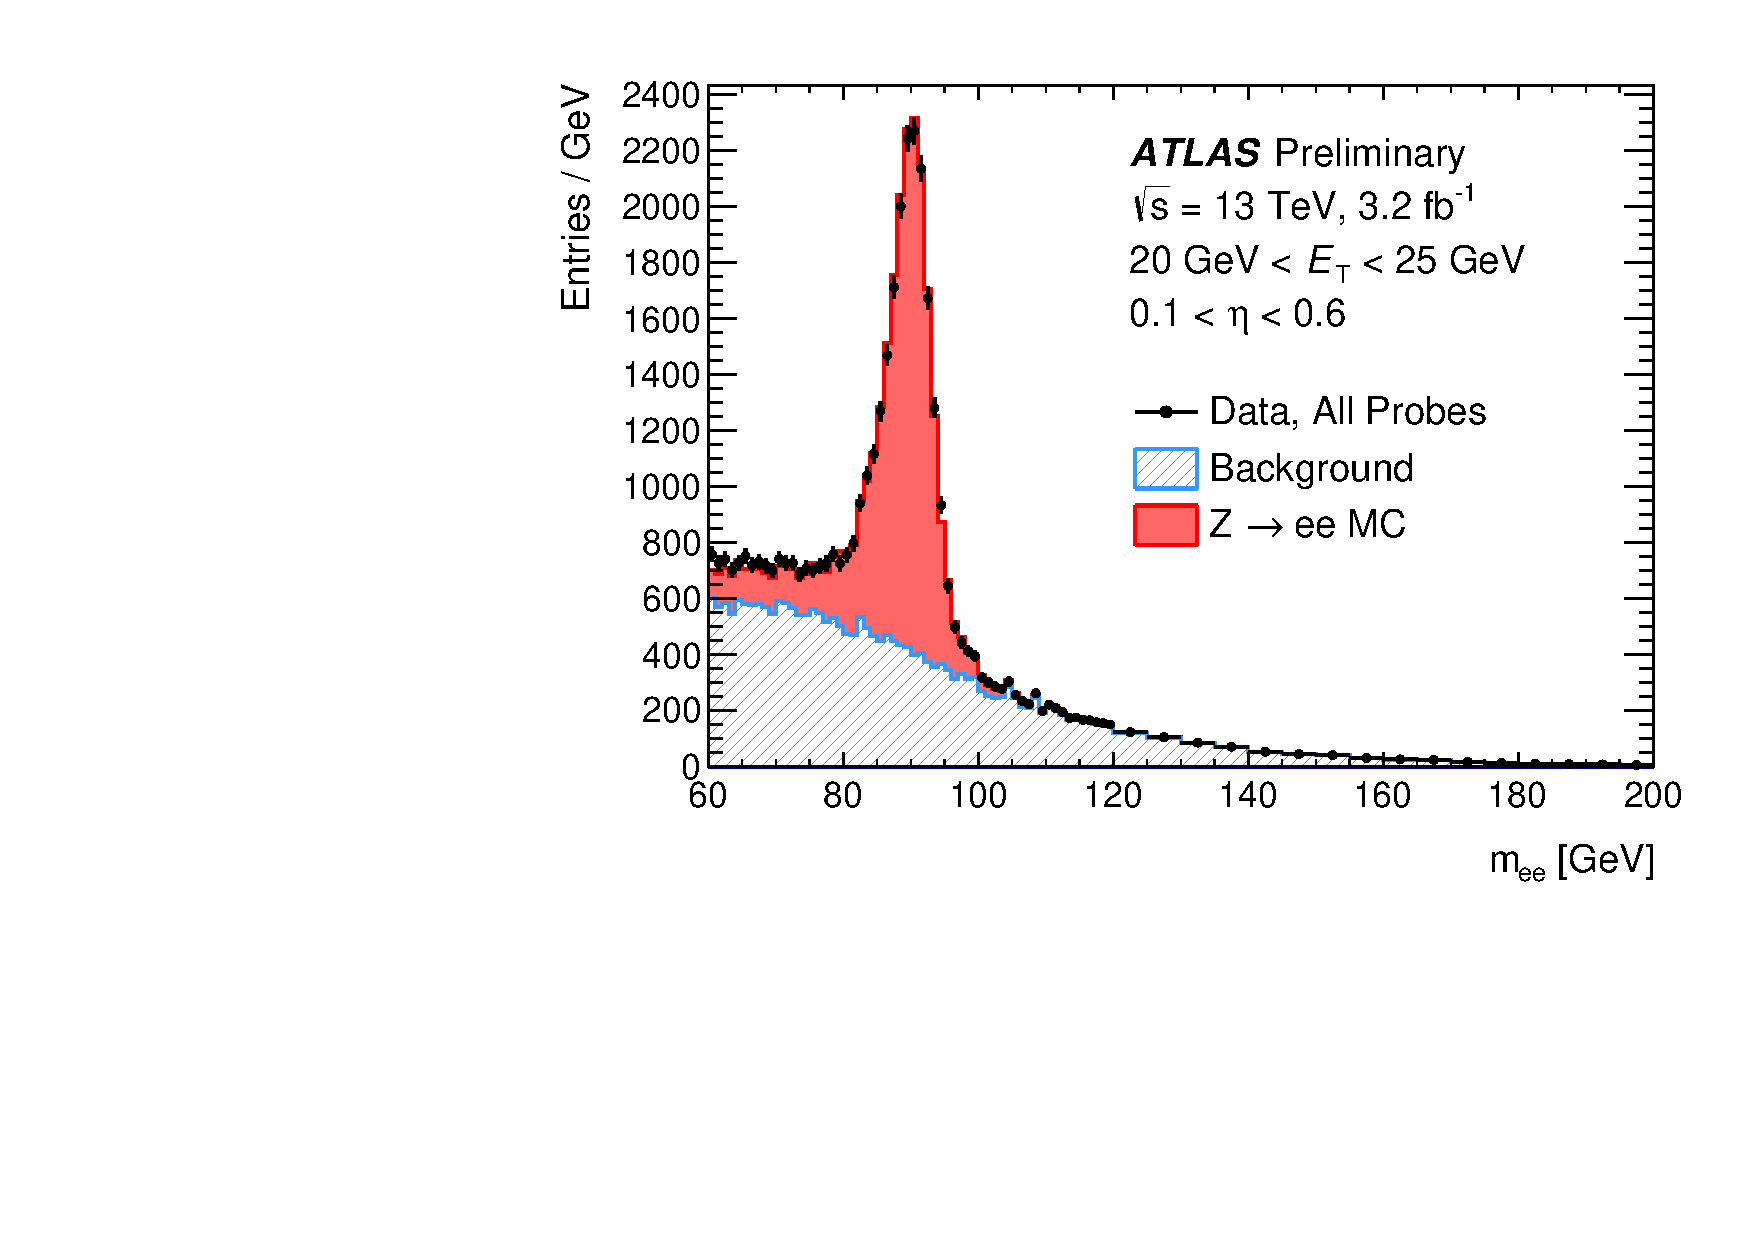
\includegraphics[scale=0.35]{fig_03a.pdf}
            \caption{The $Z_{mass}$ method}
        \end{center}
    \end{subfigure}
    \begin{subfigure}[b]{0.48\textwidth}
        \begin{center}
            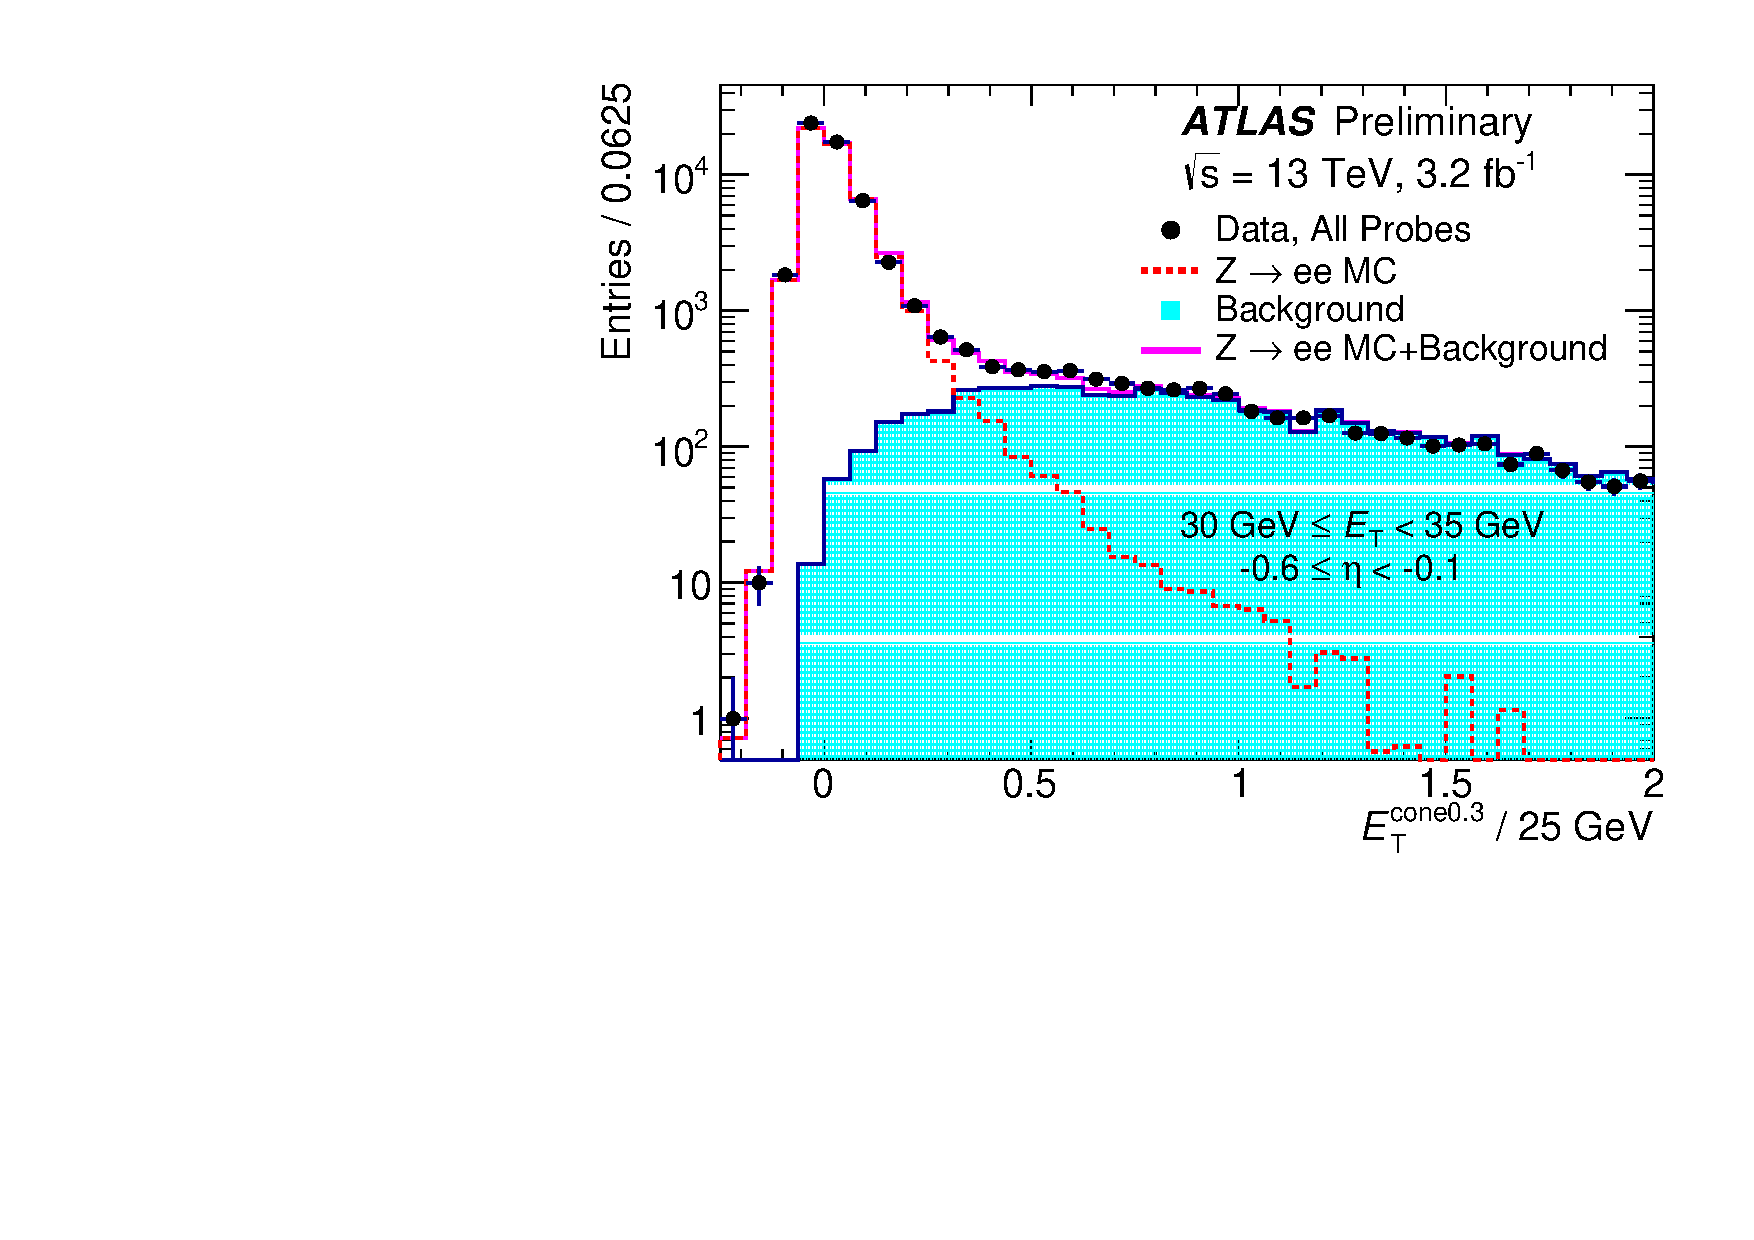
\includegraphics[scale=0.35]{fig_04a.pdf}
            \caption{The $Z_{iso}$ method}
        \end{center}
    \end{subfigure}
    \caption{Illustration of the background estimations use (a) the $Z_{mass}$ and (b) the $Z_{iso}$ methods~\cite{ATLAS:2016iqc}.}
    \label{fig:app_electron_isolation_Zee_background_subtraction_methods}
\end{figure}

The electrons in $J/\Psi$ samples have prompt and non-prompt components.
The prompt electron comes from the prompt production of $J/\Psi$ which comes from the $pp$ collisions and the non-prompt one arises from the non-prompt production of $J/\Psi$ which comes from $b$ decay.
Prompt electrons are expected more isolated than the non-prompt ones.
By using this distinguish feature, a tag-and-probe pair can be constructed.
There are two background estimation methods: short-$\tau$ and $\tau$-fit methods.
The short-$\tau$ method uses events with short pseudo-proper time to find the prompt electron.
The $\tau$-fit method considers the full $\tau$-range to extract the non-prompt electron by fitting the pseudo-proper time distribution.
Figure~\ref{fig:app_electron_isolation_JPsi_background_subtraction_methods} shows the background estimations using the short-$\tau$ and $\tau$-fit methods.
In the electron isolation, the $Z \to ee$ samples and $Z_{mass}$ method are used.

\begin{figure}[htbp]
    \begin{subfigure}[b]{0.48\textwidth}
        \begin{center}
            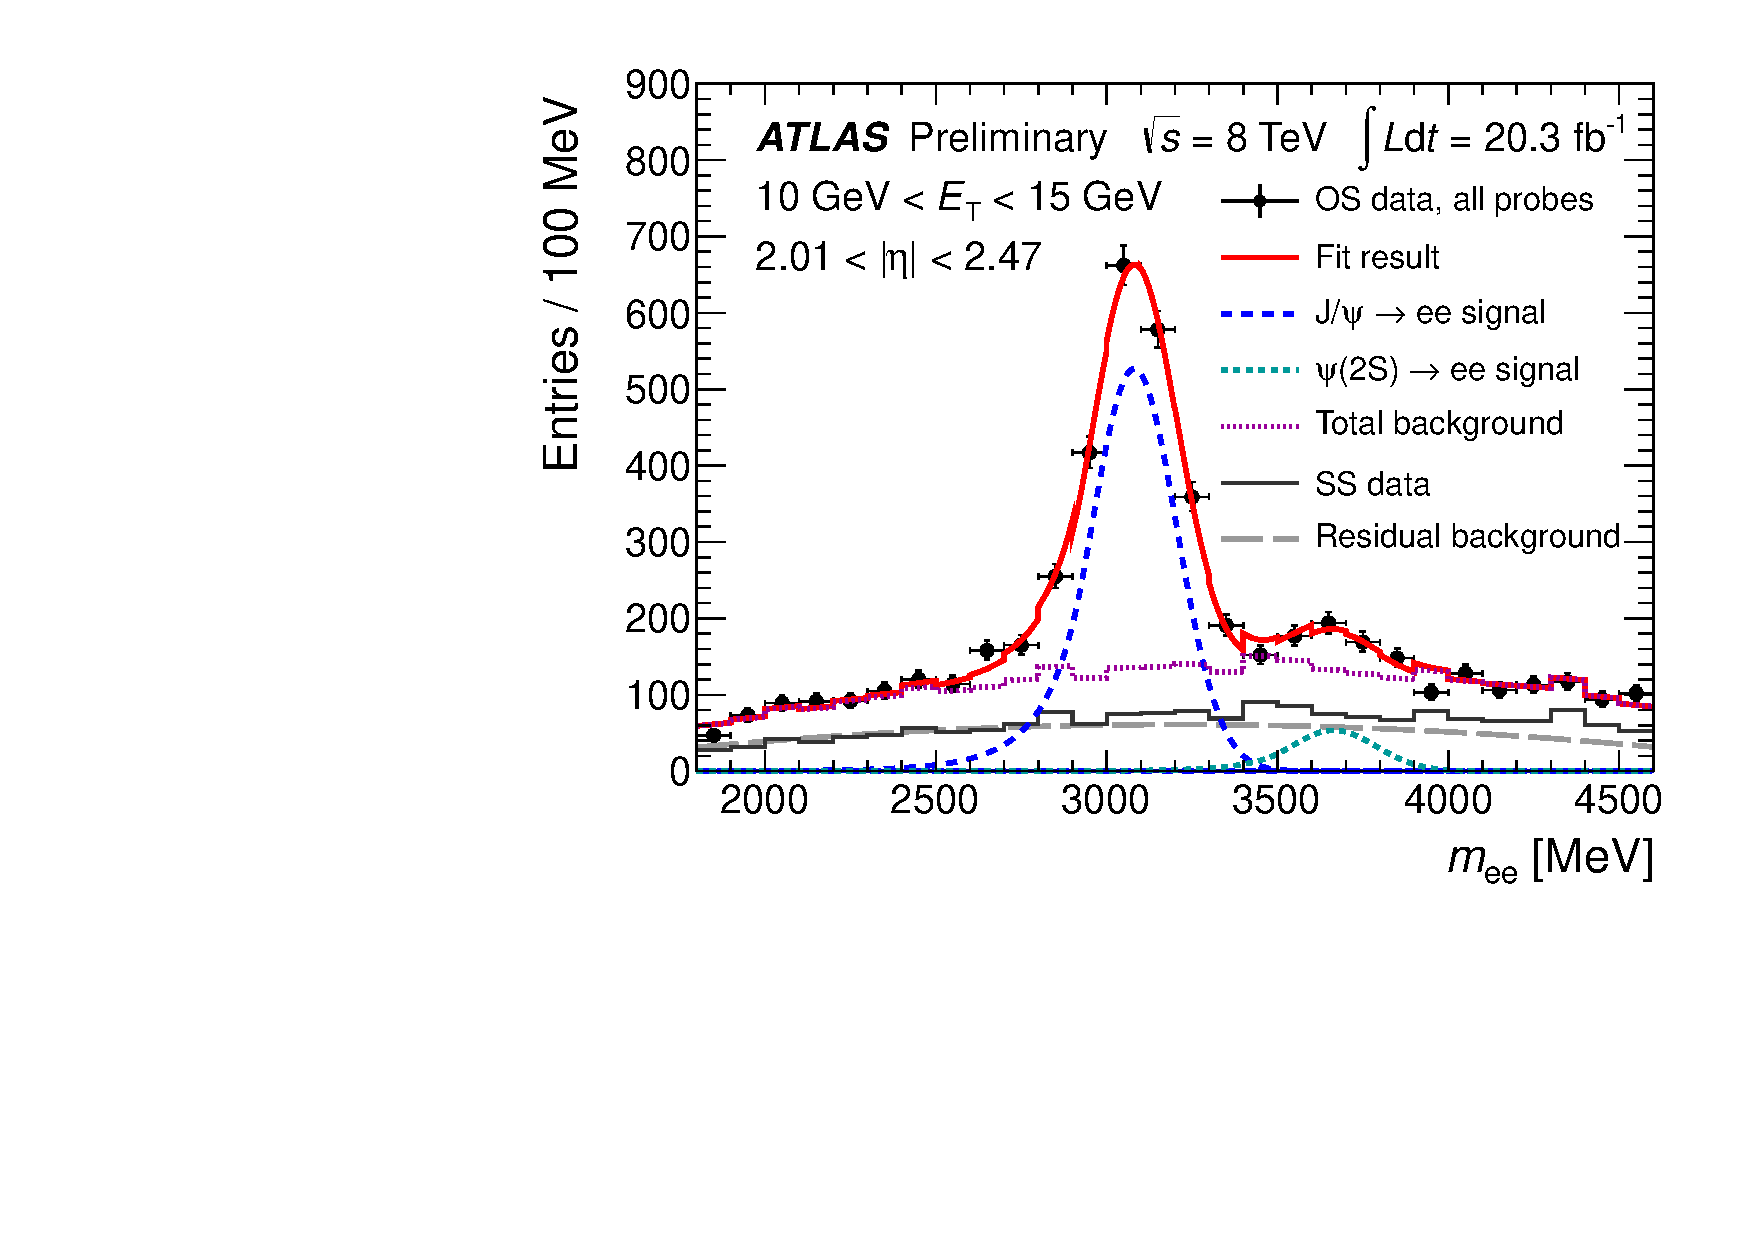
\includegraphics[scale=0.35]{fig_07a.pdf}
            \caption{The short-$\tau$ method}
        \end{center}
    \end{subfigure}
    \begin{subfigure}[b]{0.48\textwidth}
        \begin{center}
            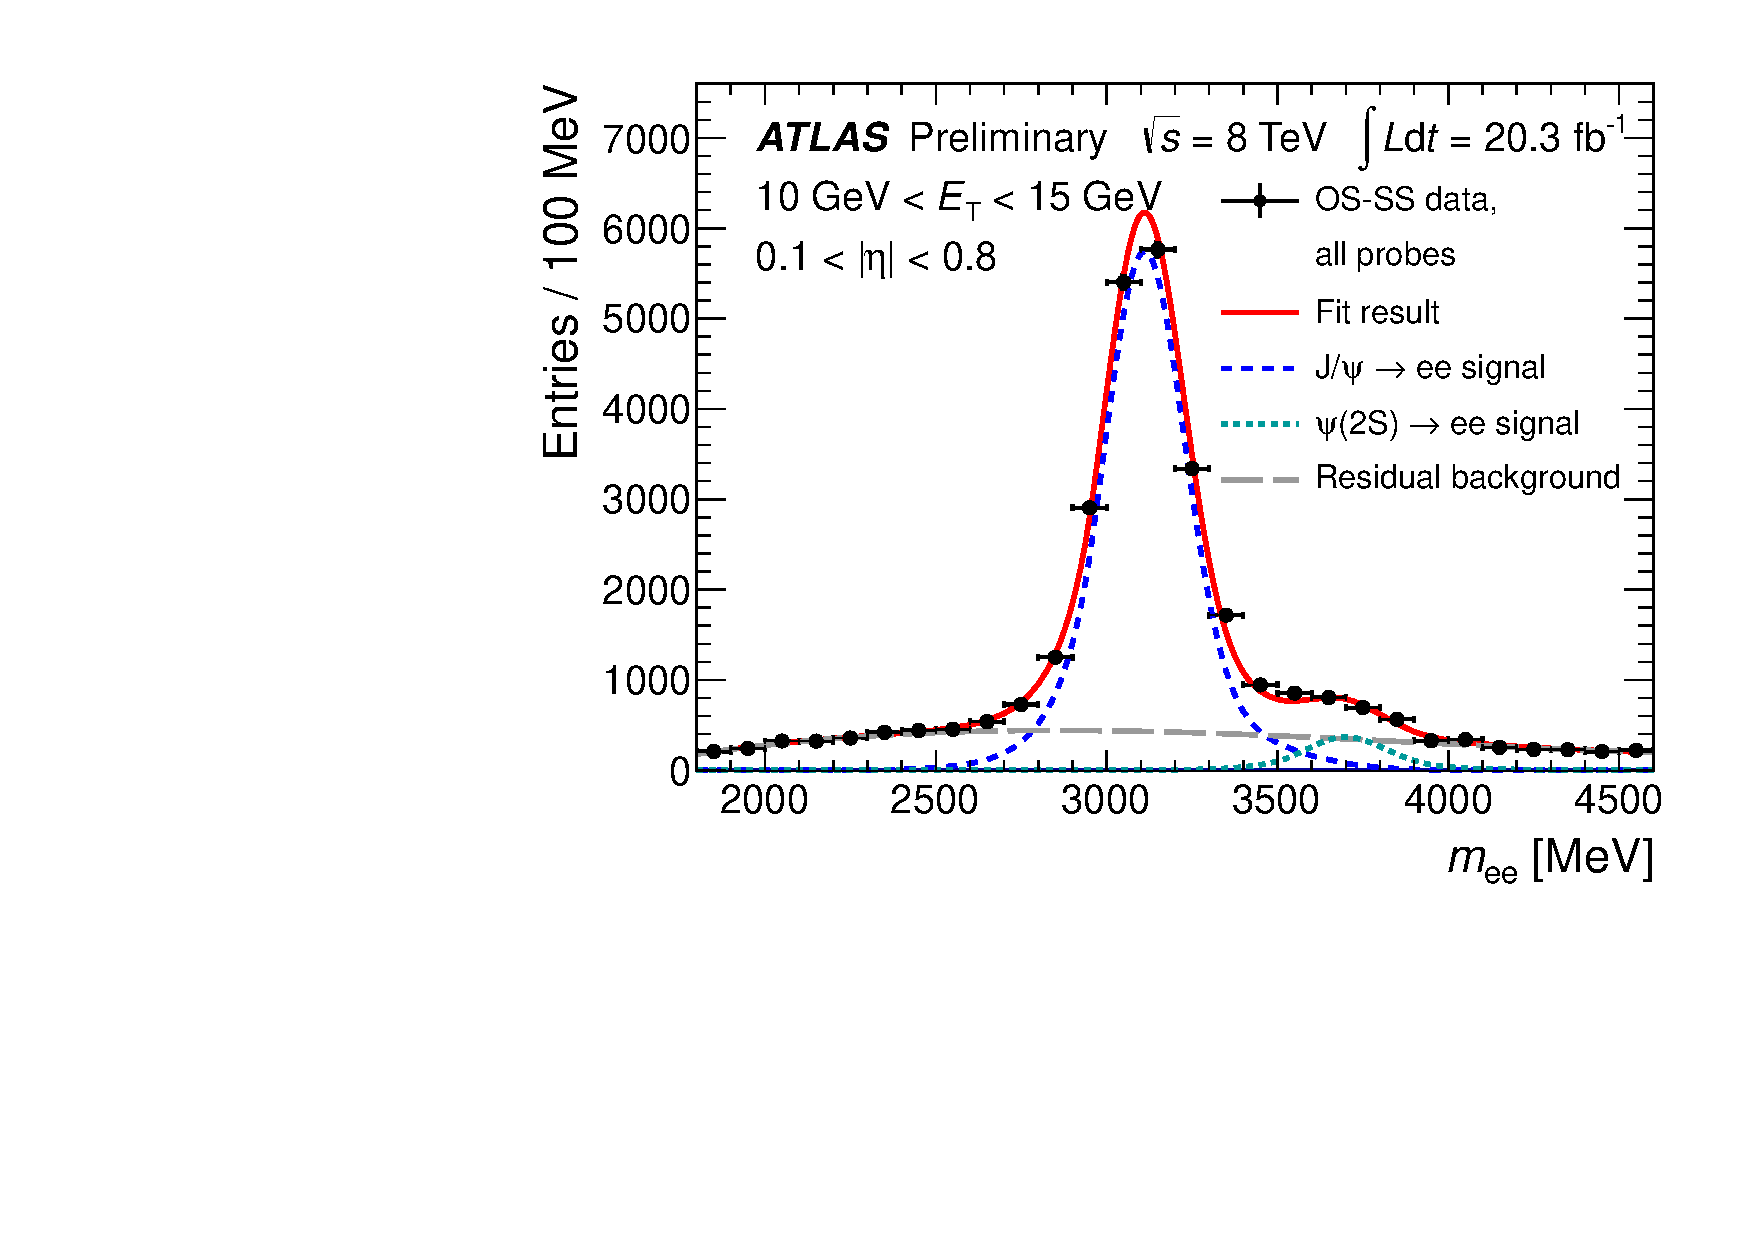
\includegraphics[scale=0.35]{fig_08a.pdf}
            \caption{The $\tau$-fit method}
        \end{center}
    \end{subfigure}
    \caption{Illustration of the background estimations use (a) the short-$\tau$ and (b) the $\tau$-fit methods~\cite{Aaboud:2016vfy}.}
    \label{fig:app_electron_isolation_JPsi_background_subtraction_methods}
\end{figure}

%%%
%%%
%%%

\section{Electron reconstruction and identification}
\label{sec:app_electron_reconstruction_and_identification}
Electron candidates are reconstructed in the central region of the ATLAS detector ($|\eta| < 2.47$) using information from the inner detector and ECAL.
Then the electron identification (ID) algorithms are used to distinguish signal or background-like candidates based on multivariate likelihood discriminant.
Signal-like electrons should be prompt and isolated.
Background-like electrons coming from photon conversions, hadronic jets misidentification, and heavy flavor decays are non-prompt.
The IBL added for Run-2 provides good discrimination between electrons and converted photons.
Three electron ID operating points \texttt{Tight}, \texttt{Medium}, and \texttt{Loose} are provided.
The \texttt{Tight} ID provides the highest background rejection power, the \texttt{Loose} has the lowest background rejection power, and \texttt{Medium} ID in between.
Figure~\ref{fig:app_electron_isolation_schematic_view_of_electron_reco_ID} shows a schematic view of the electron reconstruction and identification.
The electron reconstruction and identification efficiencies for 2016 data corresponding 33.9~\ifb are shown in Fig.~\ref{fig:app_electron_isolation_2016_electron_ID_efficiencies}.

\begin{figure}[htbp]
    \begin{center}
        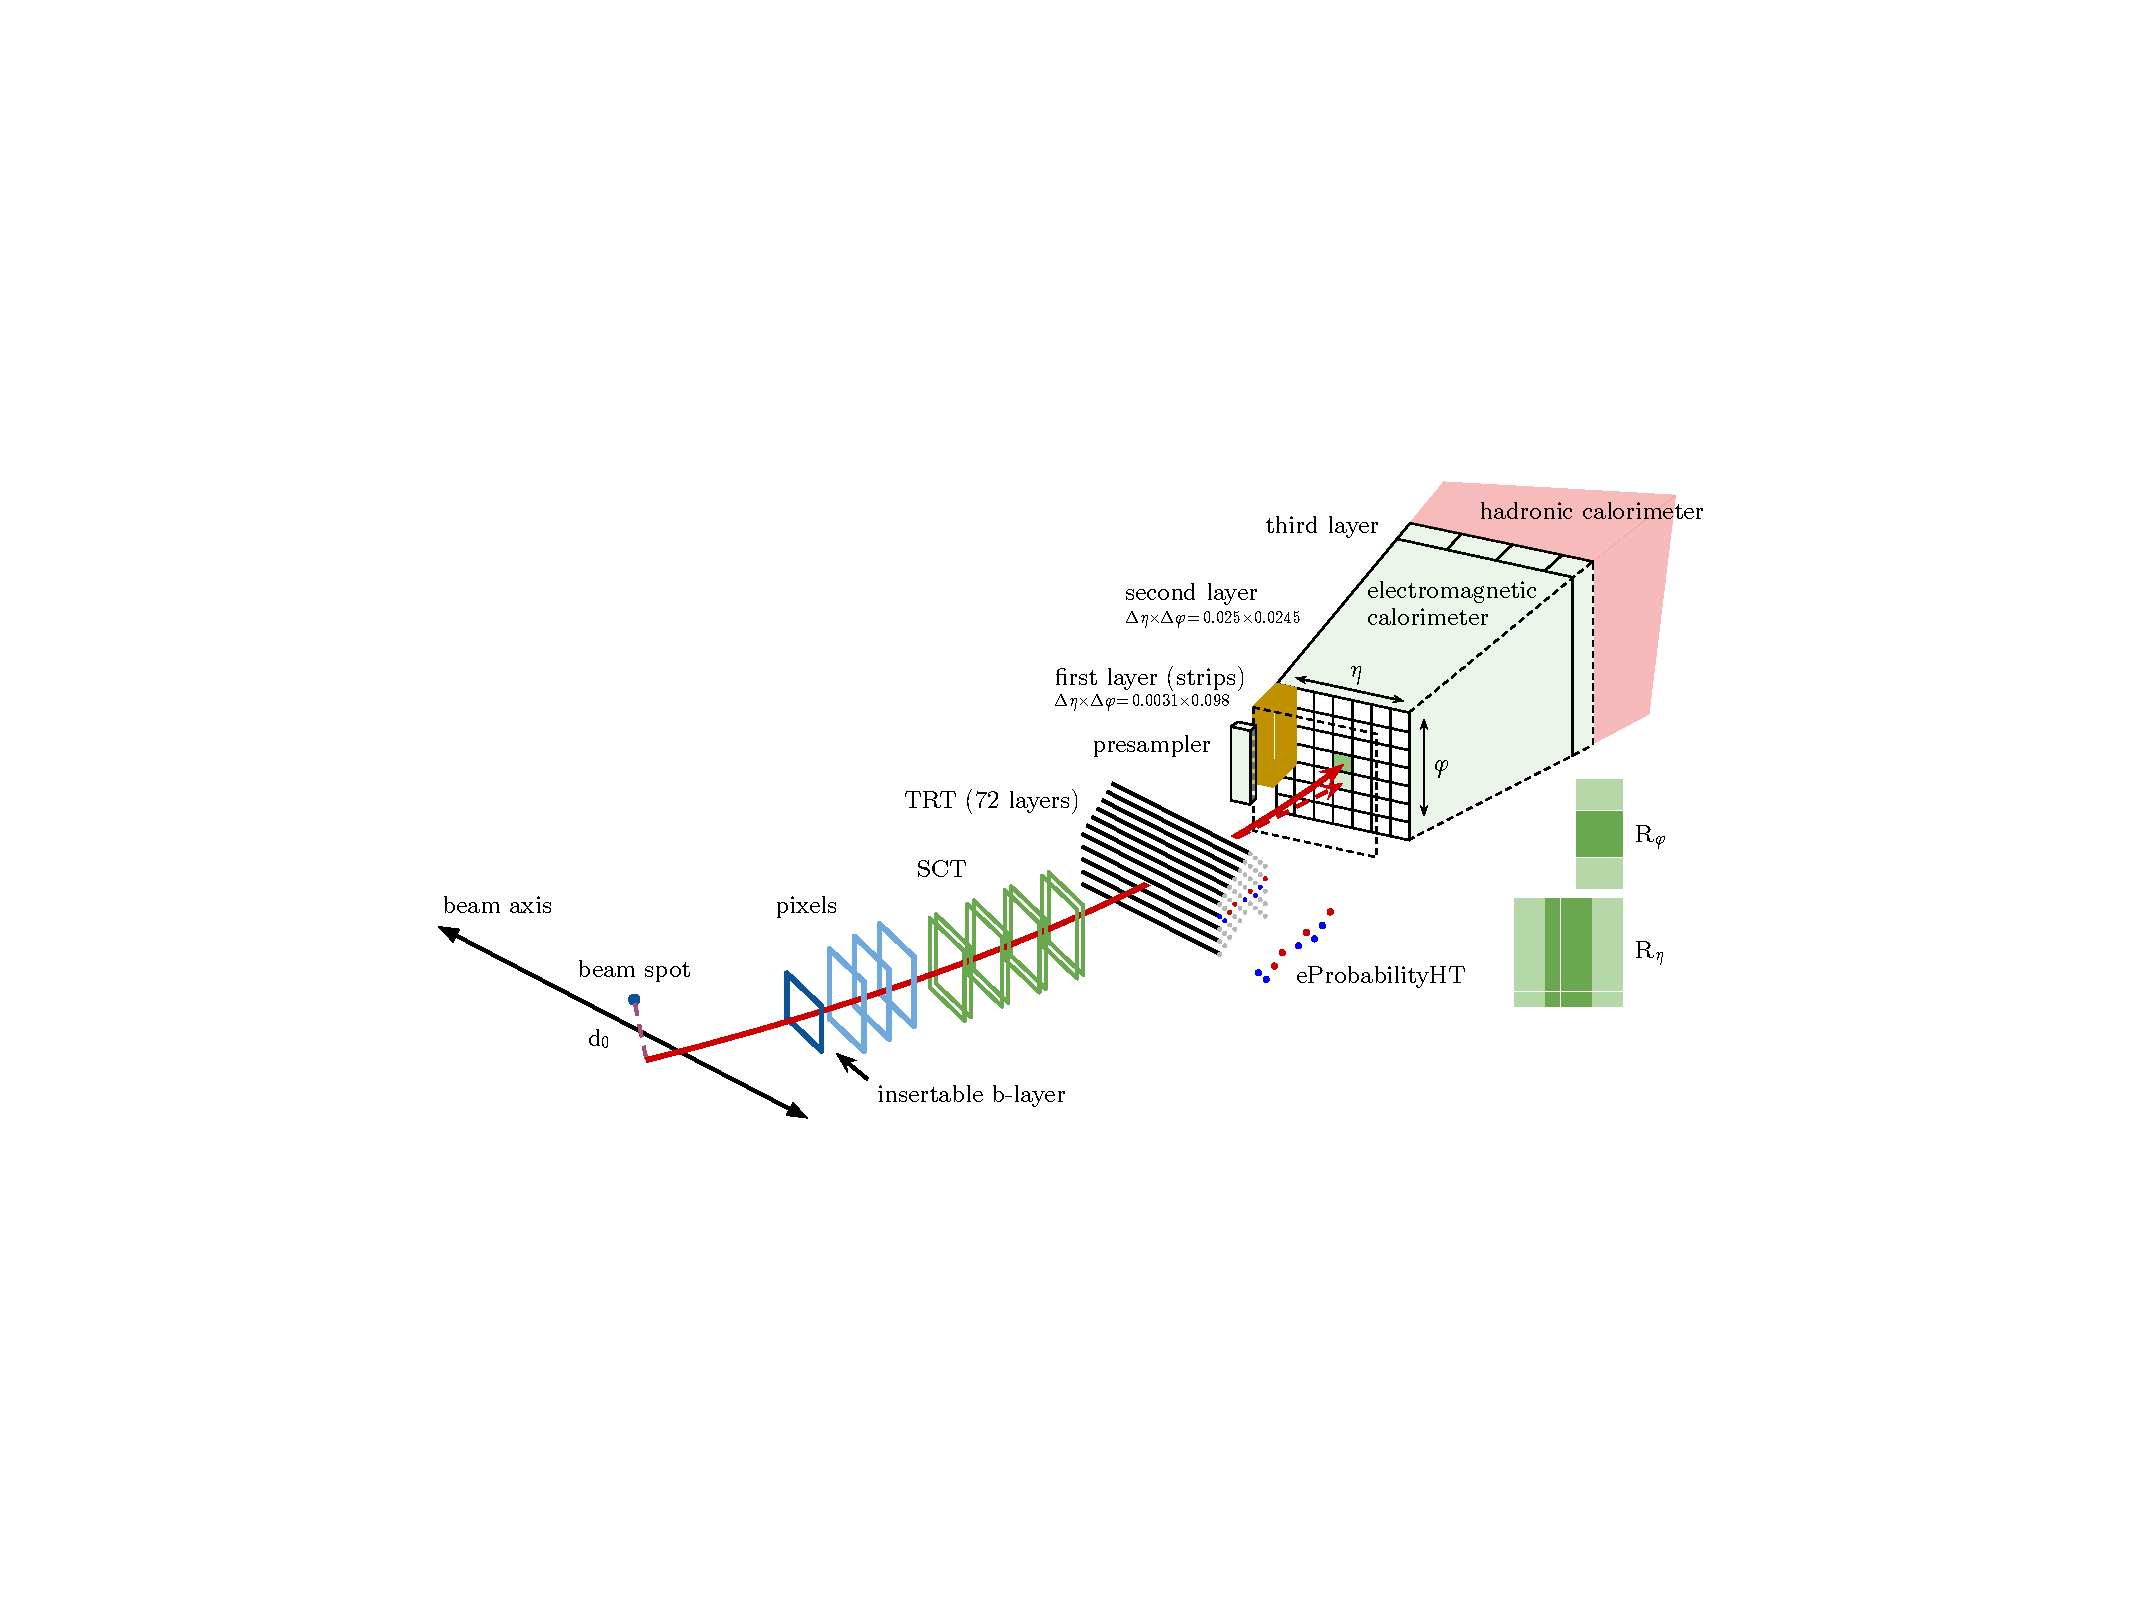
\includegraphics[scale=0.6]{figaux_03.pdf}
        \caption{A schematic view of the electron reconstruction and identification~\cite{ATLAS:2016iqc}.}
        \label{fig:app_electron_isolation_schematic_view_of_electron_reco_ID}
    \end{center}
\end{figure}

\begin{figure}[htbp]
    \begin{subfigure}[b]{0.32\textwidth}
        \begin{center}
            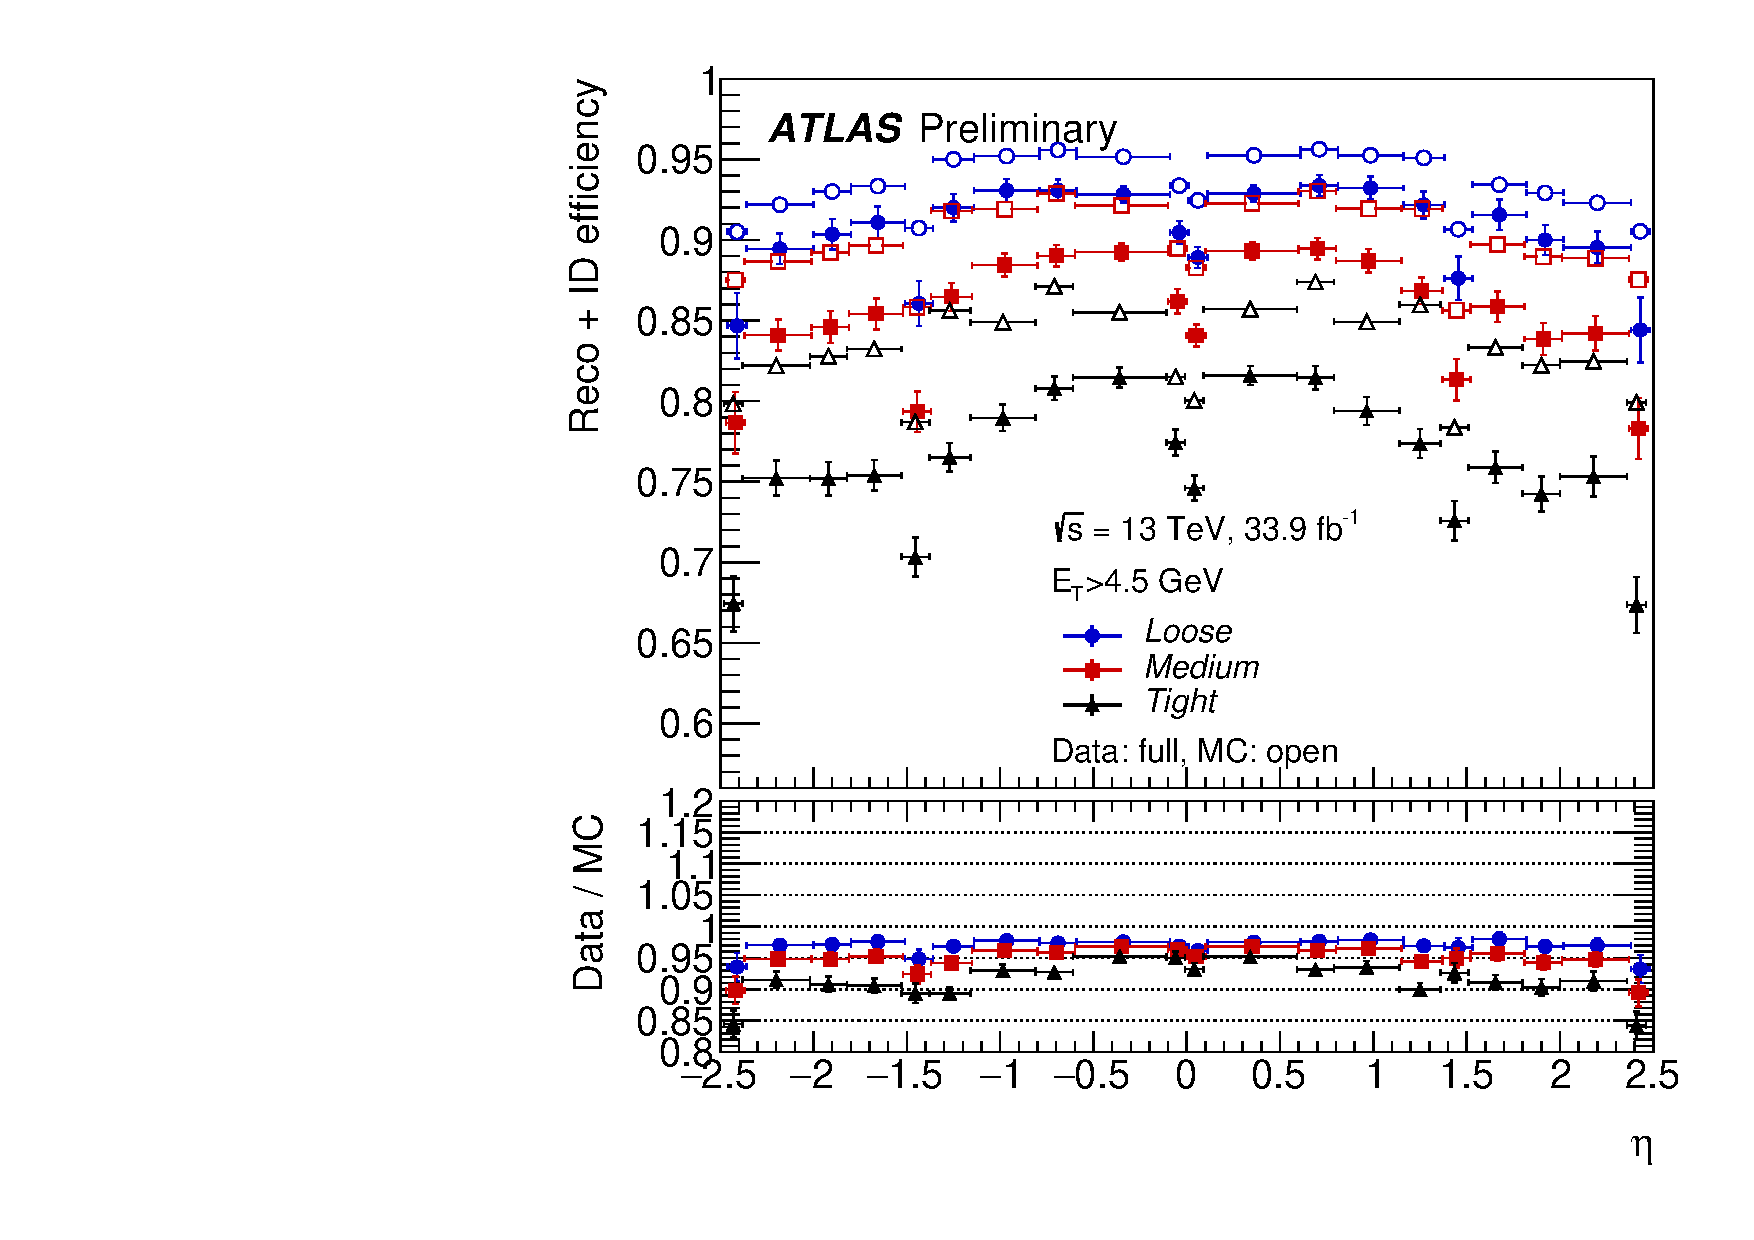
\includegraphics[scale=0.23]{fig_01.pdf}
            \caption{}
        \end{center}
    \end{subfigure}
    \begin{subfigure}[b]{0.32\textwidth}
        \begin{center}
            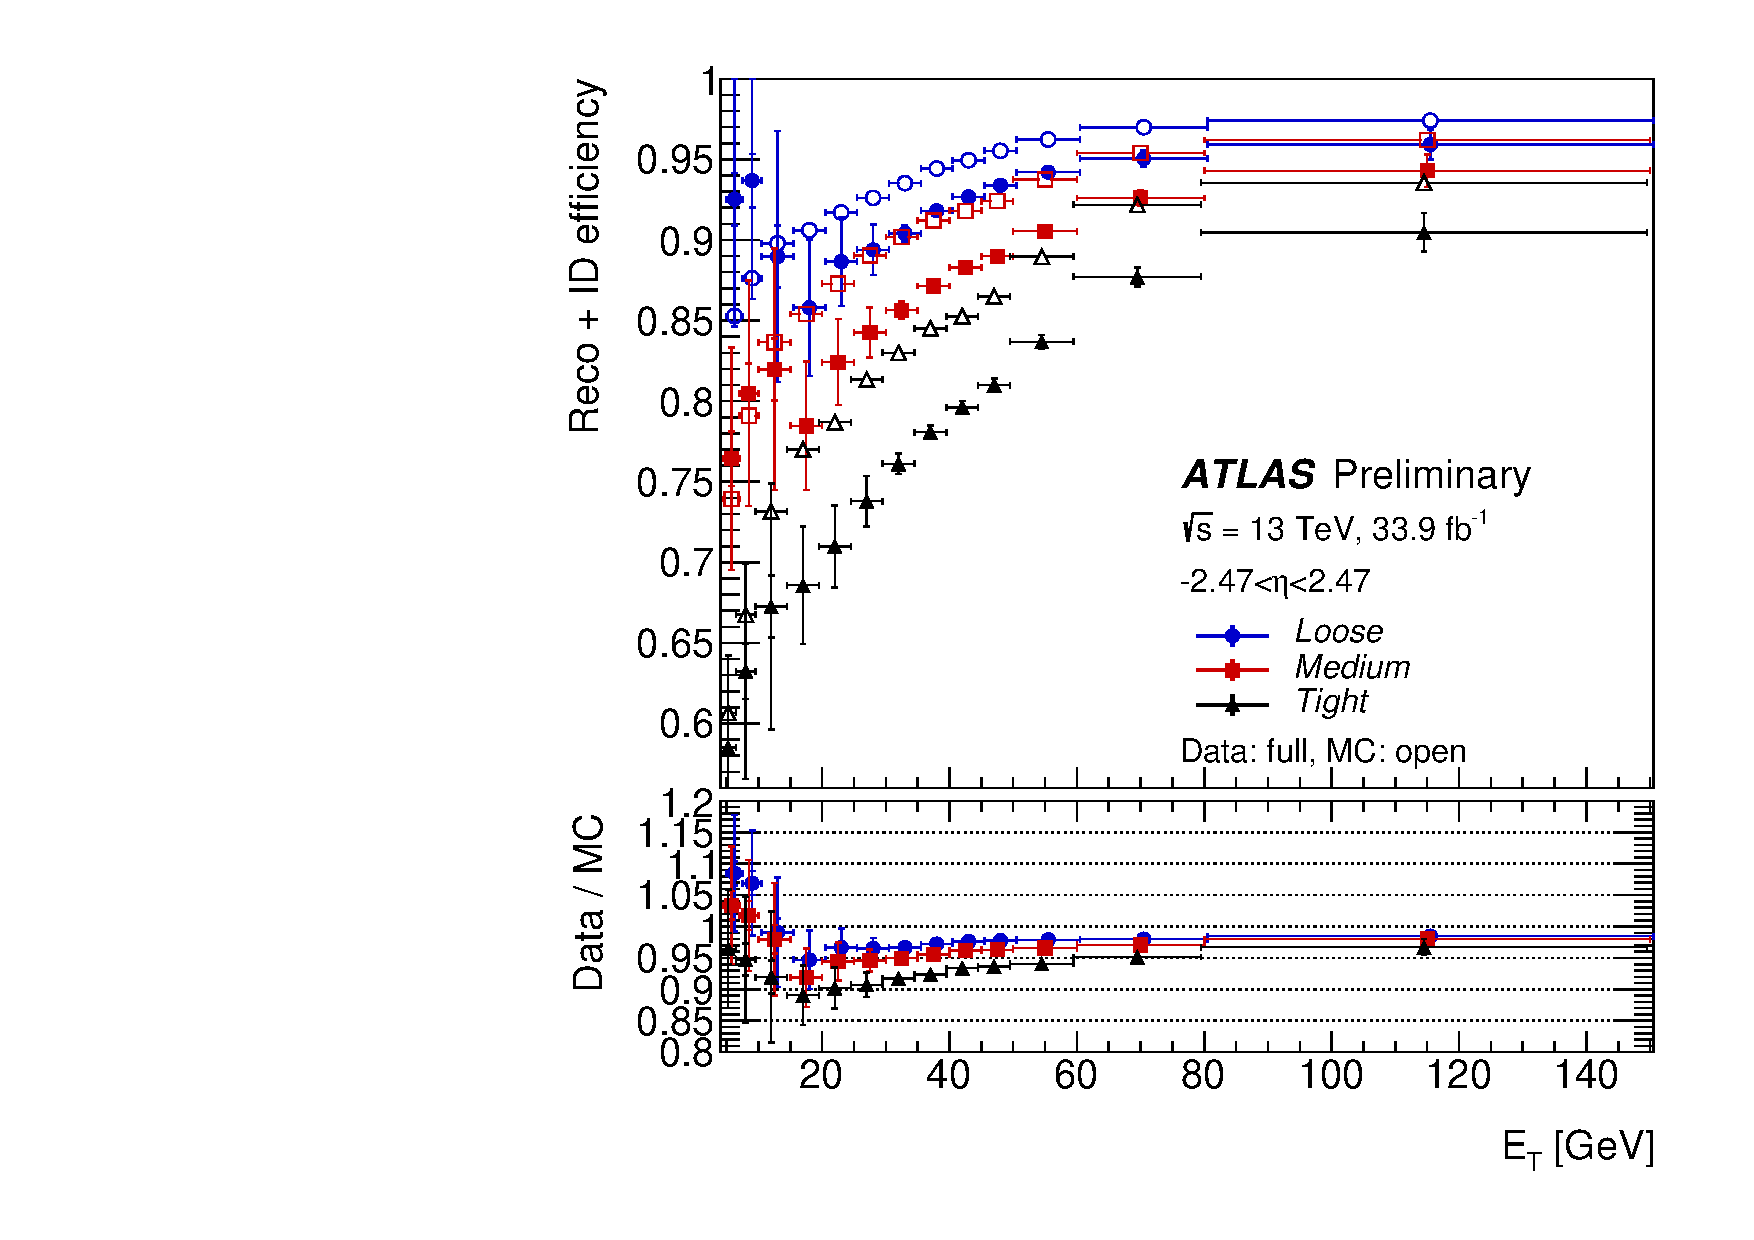
\includegraphics[scale=0.23]{fig_02.pdf}
            \caption{}
        \end{center}
    \end{subfigure}
    \begin{subfigure}[b]{0.32\textwidth}
        \begin{center}
            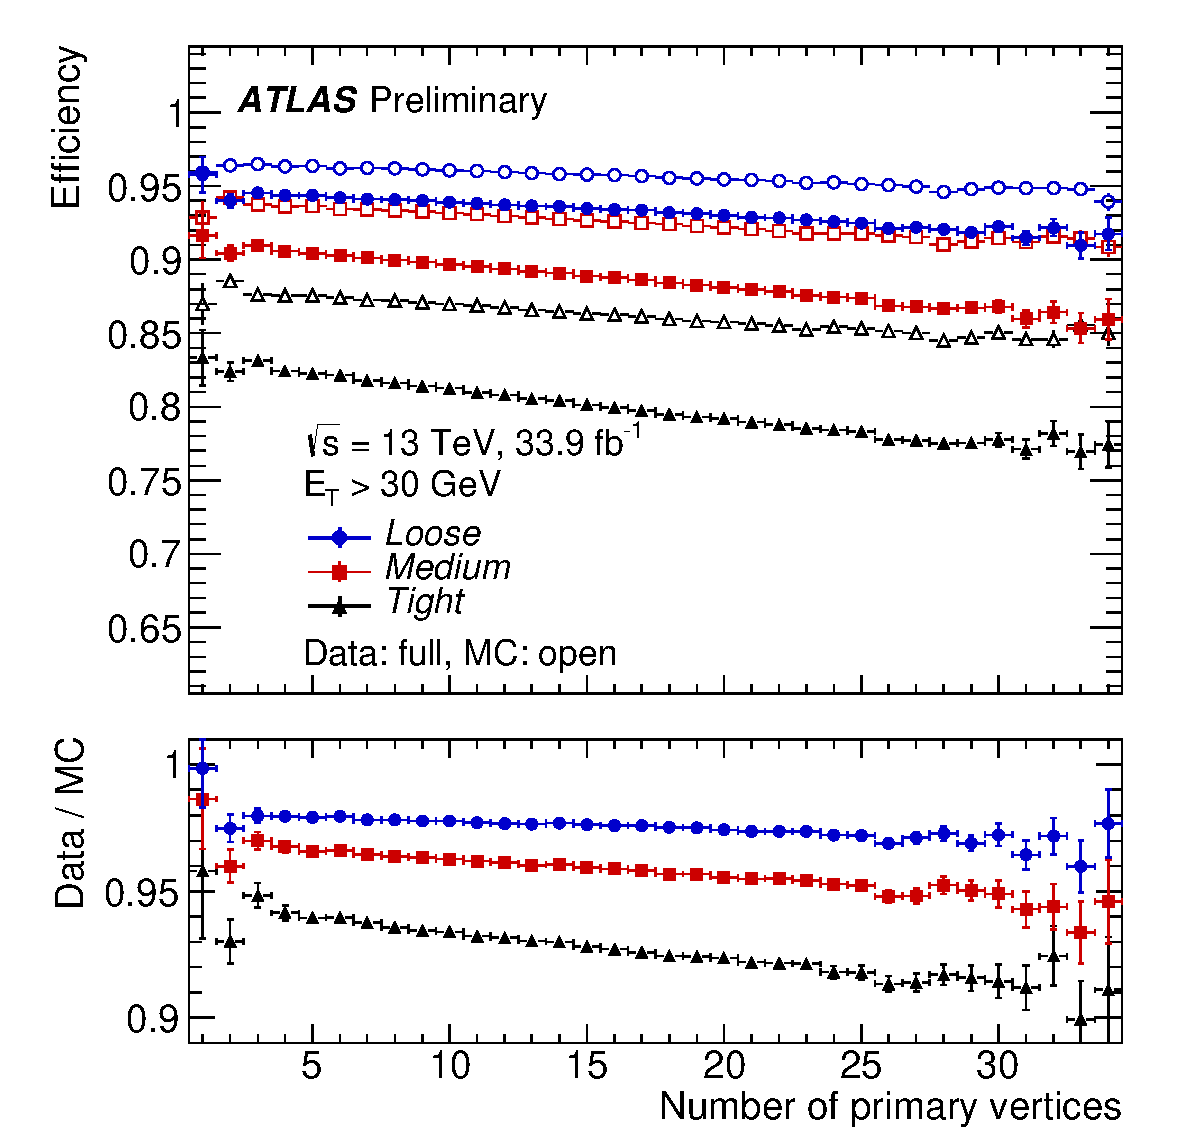
\includegraphics[scale=0.23]{fig_03.pdf}
            \caption{}
        \end{center}
    \end{subfigure}
    \caption{The electron reconstruction and identification efficiencies as a function of (a) $\eta$ and (b) \met~\cite{ATLAS:EGAM-2017-003}.
    The electron identification efficiency as a function of (c) the number of reconstructed primary vertices~\cite{ATLAS:EGAM-2016-005}.}
    \label{fig:app_electron_isolation_2016_electron_ID_efficiencies}
\end{figure}

%%%
%%%
%%%

\section{Electron isolation}
\label{sec:app_electron_isolation}
Electrons produced in the LHC $pp$ collisions cover a wide range of \met from a few {\GeV} to several {\TeV}.
Reconstructed electrons suffer large backgrounds from misidentified hadrons, photon conversions, and heavy-flavor decays.
In order to further discriminate signal and background, most analyses require electrons to be isolated in addition to the identification criteria.
Background electrons are produced in association with other objects such as jets, therefore they have larger values of isolation. 
However, signal electrons tend to have low values of isolation as they are uncorrelated with other jet activities in the event.
The isolation variables quantify the energy deposited in a cone centered around the electron candidates and allow prompt electrons to be disentangled from non-isolated electrons.
Hence, electron isolation is a very powerful tool to reject backgrounds.
Two discriminating variables have been designed for that purpose: a calorimetric isolation energy $E_\mathrm{T}^\mathrm{cone\ 0.2}$ and a track isolation $p_\mathrm{T}^\mathrm{varcone\ 0.2}$.
The $E_\mathrm{T}^\mathrm{cone\ 0.2}$ is defined as the sum of transverse energies of topological clusters~\cite{Aad:2016upy} within a cone of $\Delta R = 0.2$ around the candidate electron cluster and excluding the contribution in a region $\Delta \eta \times \Delta \phi = 0.125 \times 0.175$ centered around the electron cluster barycenter.
Only clusters with positive $E_\mathrm{T}$ are considered in the sum.
The energy leakage outside the clusters, pileup contributions, and the underlying event activity are corrected. 
The $p_\mathrm{T}^\mathrm{varcone\ 0.2}$ is defined as the sum of transverse momenta of all tracks within a cone of $\Delta R = \mathrm{min}(0.2, 10~{\GeV}/E_\mathrm{T})$ around the candidate electron track and originating from the reconstructed primary vertex of the hard collision.
The track must satisfy $E_\mathrm{T} > 1$~{\GeV}, $|\Delta z_{0} \sin \theta| < 3$~mm, and $n_\mathrm{Si} \ge 7$, $n_\mathrm{Si}^\mathrm{hole} \le 2$, $n_\mathrm{pixel}^\mathrm{hole} \le 1$, and $n_\mathrm{mod}^\mathrm{sh} \le 1$, where $n_\mathrm{Si}^\mathrm{hole}$ and $n_\mathrm{pixel}^\mathrm{hole}$ are the number of missing hits in the silicon and pixel detector respectively and $n_\mathrm{mod}^\mathrm{sh}$ is the number of hits in the silicon detector assigned to more than one track.
The distributions of $E_\mathrm{T}^\mathrm{cone\ 0.2}$ and $p_\mathrm{T}^\mathrm{varcone\ 0.2}$ are shown in Fig.~\ref{fig:app_electron_isolation_ETcone20_PTvarcone20}.

\begin{figure}[htbp]
    \begin{subfigure}[b]{0.48\textwidth}
        \begin{center}
            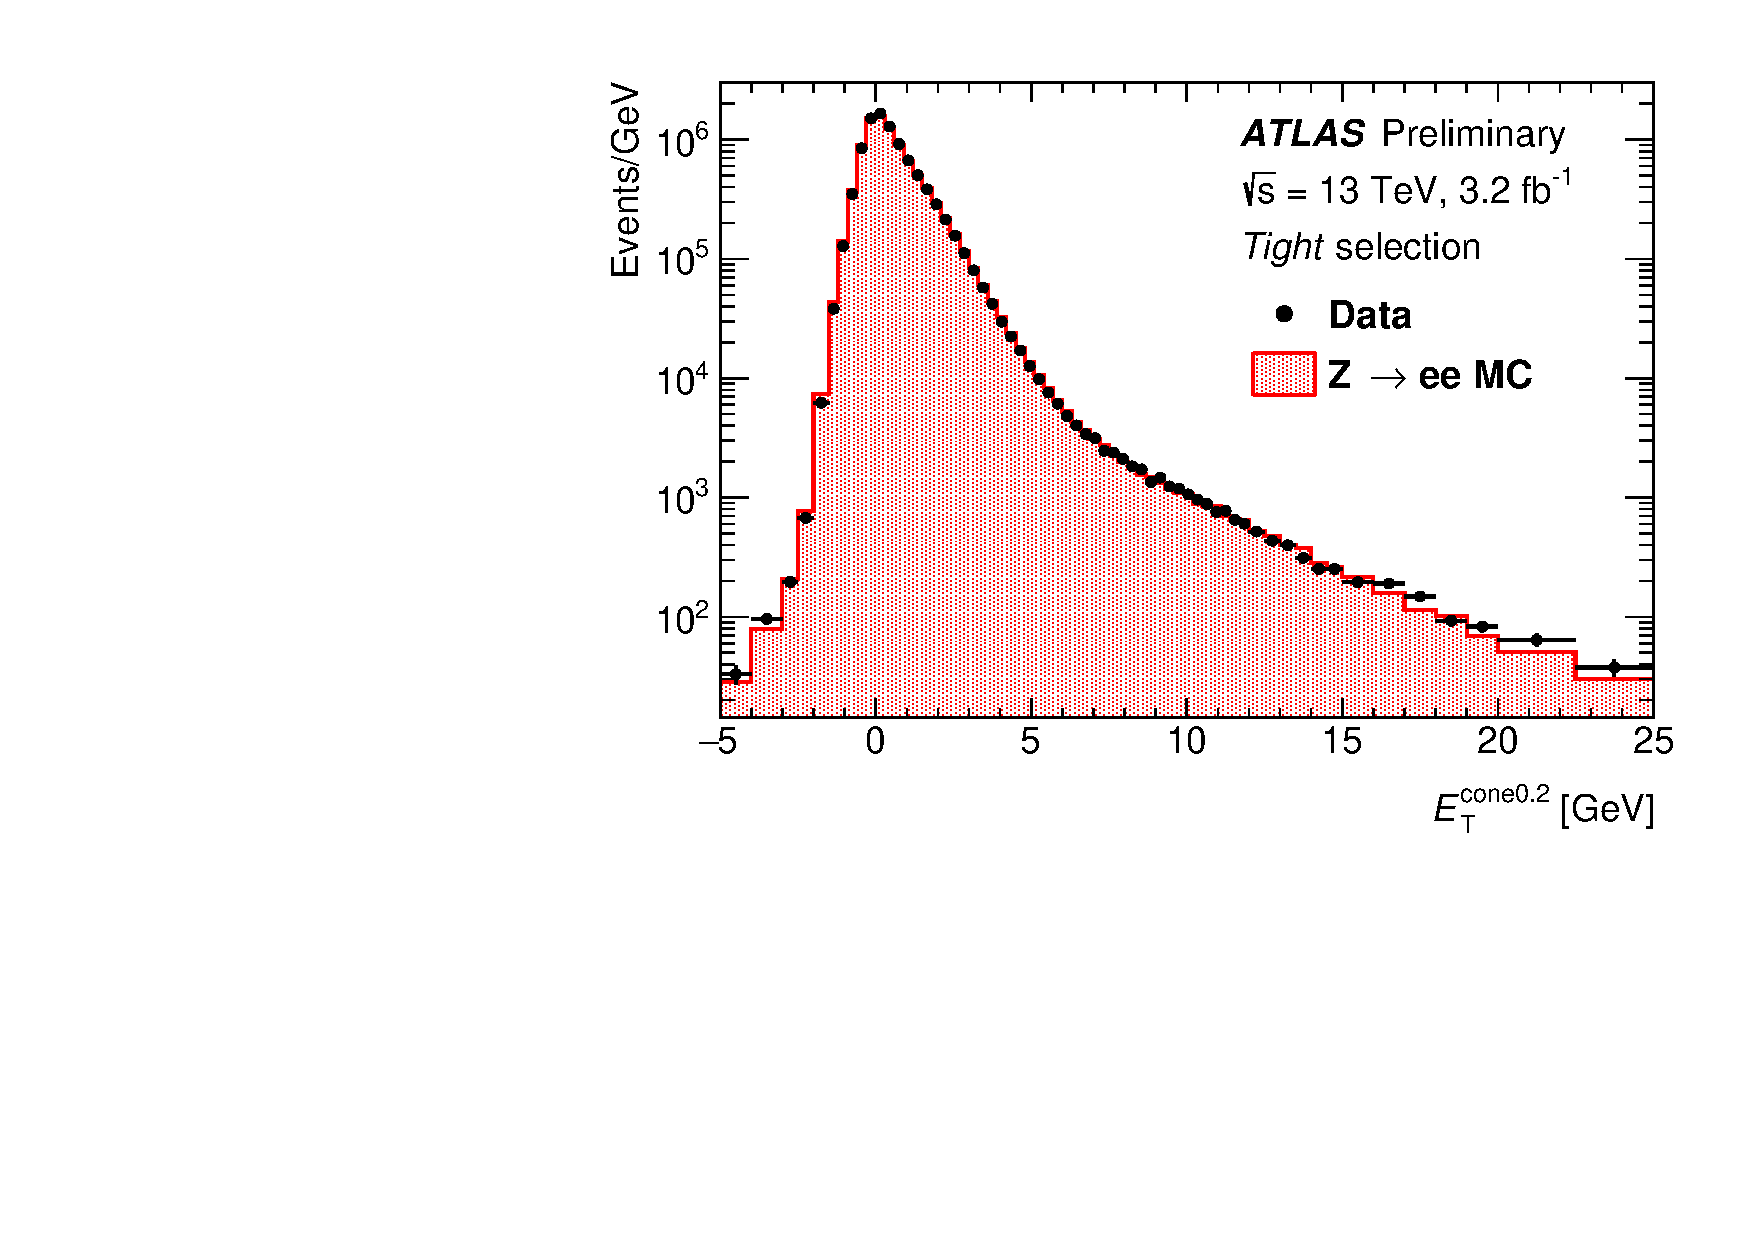
\includegraphics[scale=0.35]{fig_02a.pdf}
            \caption{$E_\mathrm{T}^\mathrm{cone\ 0.2}$}
        \end{center}
    \end{subfigure}
    \begin{subfigure}[b]{0.48\textwidth}
        \begin{center}
            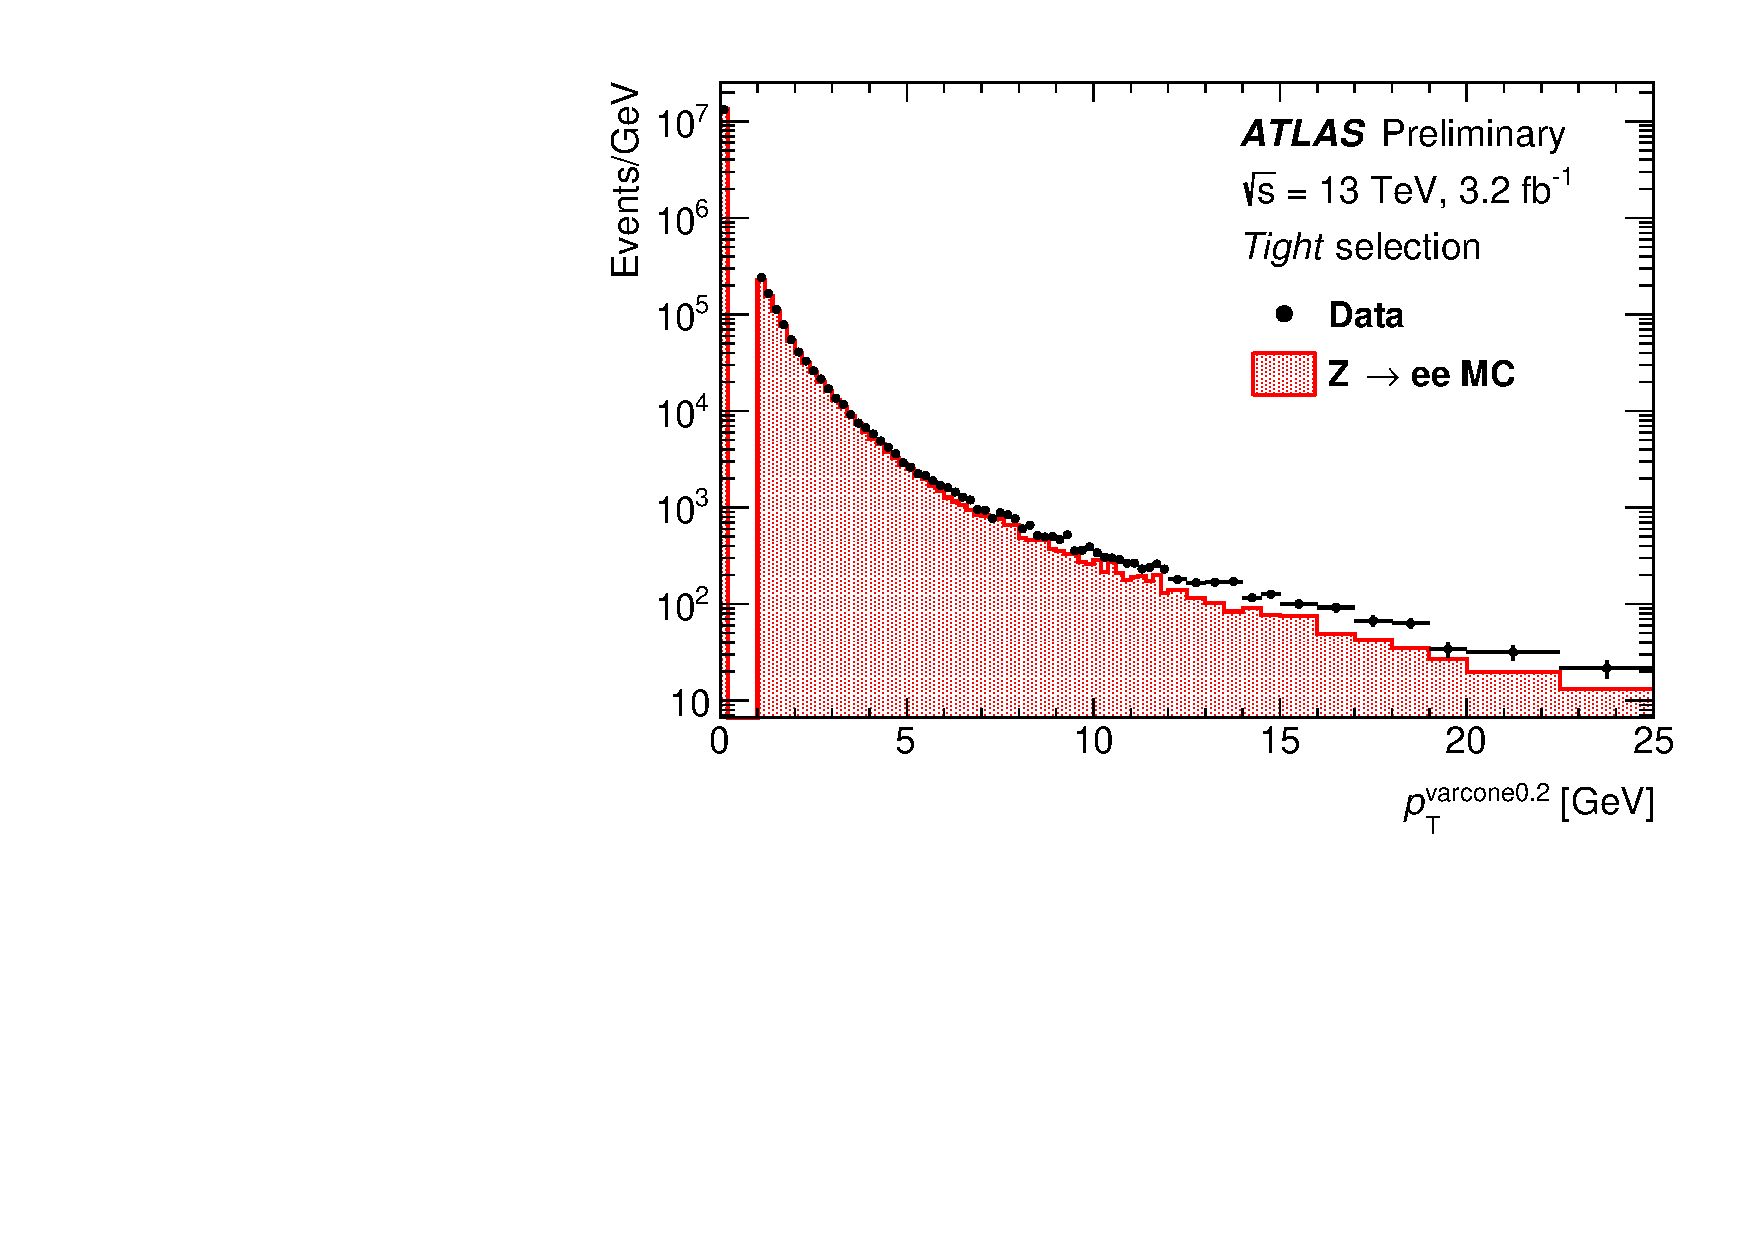
\includegraphics[scale=0.35]{fig_02b.pdf}
            \caption{$p_\mathrm{T}^\mathrm{varcone\ 0.2}$}
        \end{center}
    \end{subfigure}
    \caption{The (a) $E_\mathrm{T}^\mathrm{cone\ 0.2}$ and (b) $p_\mathrm{T}^\mathrm{varcone\ 0.2}$ distributions~\cite{ATLAS:2016iqc}.
    The negative tail of $E_\mathrm{T}^\mathrm{cone\ 0.2}$ originates from the correction for pileup and the underlying event activity.
    No background subtraction is applied in the plots, so a slight discrepancy is observed in the region at large $E_\mathrm{T}^\mathrm{cone\ 0.2}$ and $p_\mathrm{T}^\mathrm{varcone\ 0.2}$ values where the background dominates.}
    \label{fig:app_electron_isolation_ETcone20_PTvarcone20}
\end{figure}

Table~\ref{tab:app_electron_isolation_working_points} lists the electron isolation working points, which are various selection requirements on the $E_\mathrm{T}^\mathrm{cone\ 0.2}$ and $p_\mathrm{T}^\mathrm{varcone\ 0.2}$, to select isolated electron candidates.
The \texttt{Tight}, \texttt{Loose}, \texttt{LooseTrackOnly}, \texttt{Gradient}, and \texttt{GradientLoose} are the efficiency targeted working points.
By applying various requirements, the isolation efficiency $\epsilon_{iso}$ can be obtained.
The \texttt{FixedCutTightTrackOnly}, \texttt{FixedCutTight}, and \texttt{FixedCutLoose} are the fixed requirement working points.
The upper thresholds on the isolation variables are constant.
The fixed requirement working points are used in analyses with low $E_\mathrm{T}$ electrons and require high background rejection.

\begin{table}[htbp]
    \begin{center}
        \resizebox{\textwidth}{!}{%
            {\footnotesize
                \begin{tabular}{ccccc}
                    \hline
                    \hline
                    Working point          & Calorimeter isolation                        & Track isolation                                 & Combined isolation\\
                    \hline
                    Tight                  & 96\%                                         & 99\%                                            & 95\%\\
                    Loose                  & 99\%                                         & 99\%                                            & 99\%\\
                    LooseTrackOnly         & -                                            & 99\%                                            & 99\%\\
                    \hline
                    Gradient               & $(0.1143 \times E_\mathrm{T} + 92.14)$ \%    & $(0.1143 \times E_\mathrm{T} + 92.14)$ \%       & 90\%/99\% at 25/60~{\GeV}\\
                    GradientLoose          & $(0.057 \times E_\mathrm{T} + 95.57)$ \%     & $(0.057 \times E_\mathrm{T} + 95.57)$ \%        & 95\%/99\% at 25/60~{\GeV}\\
                    \hline
                    FixedCutTightTrackOnly & -                                            & $p_\mathrm{T}^\mathrm{varcone\ 0.2}/\pt < 0.06$ & -\\
                    FixedCutTight          & $E_\mathrm{T}^\mathrm{cone\ 0.2}/\pt < 0.06$ & $p_\mathrm{T}^\mathrm{varcone\ 0.2}/\pt < 0.06$ & -\\
                    FixedCutLoose          & $E_\mathrm{T}^\mathrm{cone\ 0.2}/\pt < 0.2$  & $p_\mathrm{T}^\mathrm{varcone\ 0.2}/\pt < 0.15$ & -\\
                    \hline
                    \hline
                \end{tabular}
            }
        }
    \end{center}
    \caption{The definitions of the electron isolation working points.
    The numbers in the table represent the target efficiencies for the target working points.
    For Gradient, GradientLoose, and fixed requirement working points, the $E_\mathrm{T}$ and \pt are in {\GeV}.}
    \label{tab:app_electron_isolation_working_points}
\end{table}%

%%%
%%%
%%%

\section{The electron isolation efficiency}
\label{sec:app_electron_isolation_efficiency}
The probe electron candidates with $E_\mathrm{T} > 7$~{\GeV} are used in the electron isolation efficiency measurement.
The tag-and-probe method with $Z \to ee$ events are used for the efficiency measurement and the $Z_{mass}$ method is used to estimate background.
The isolation efficiency is defined as
%
\begin{equation}
    \epsilon_{iso} = \frac{N_{\mathrm{identification} \cap \mathrm{isolation}}}{N_\mathrm{identification}} \quad .
\end{equation}
%
The efficiencies are measured for all isolation working points listed in Table~\ref{tab:app_electron_isolation_working_points} with respect to three likelihood identifications \texttt{TightLLH}, \texttt{MediumLLH}, and \texttt{LooseLLH}.
The electron isolation efficiencies depend on the transverse energy $E_\mathrm{T}$ and pseudorapidity $\eta$.
Fig~\ref{fig:app_electron_isolation_isolation_plots} shows the electron isolation efficiencies for the fixedCutLoose working point and data-to-MC ratios as a function of the transverse energy $E_\mathrm{T}$ and pseudorapidity $\eta$, respectively.
Larger discrepancies between data and MC are observed for $E_\mathrm{T} < 20$~{\GeV} and good agreement is found when $E_\mathrm{T} > 20$~{\GeV}.
Good agreement is also observed as a function of $\eta$ with slightly larger discrepancies at the level of 1\% in the regions $|\eta| \approx 1.5$.

\begin{figure}[htbp]
    \begin{subfigure}[b]{0.48\textwidth}
        \begin{center}
            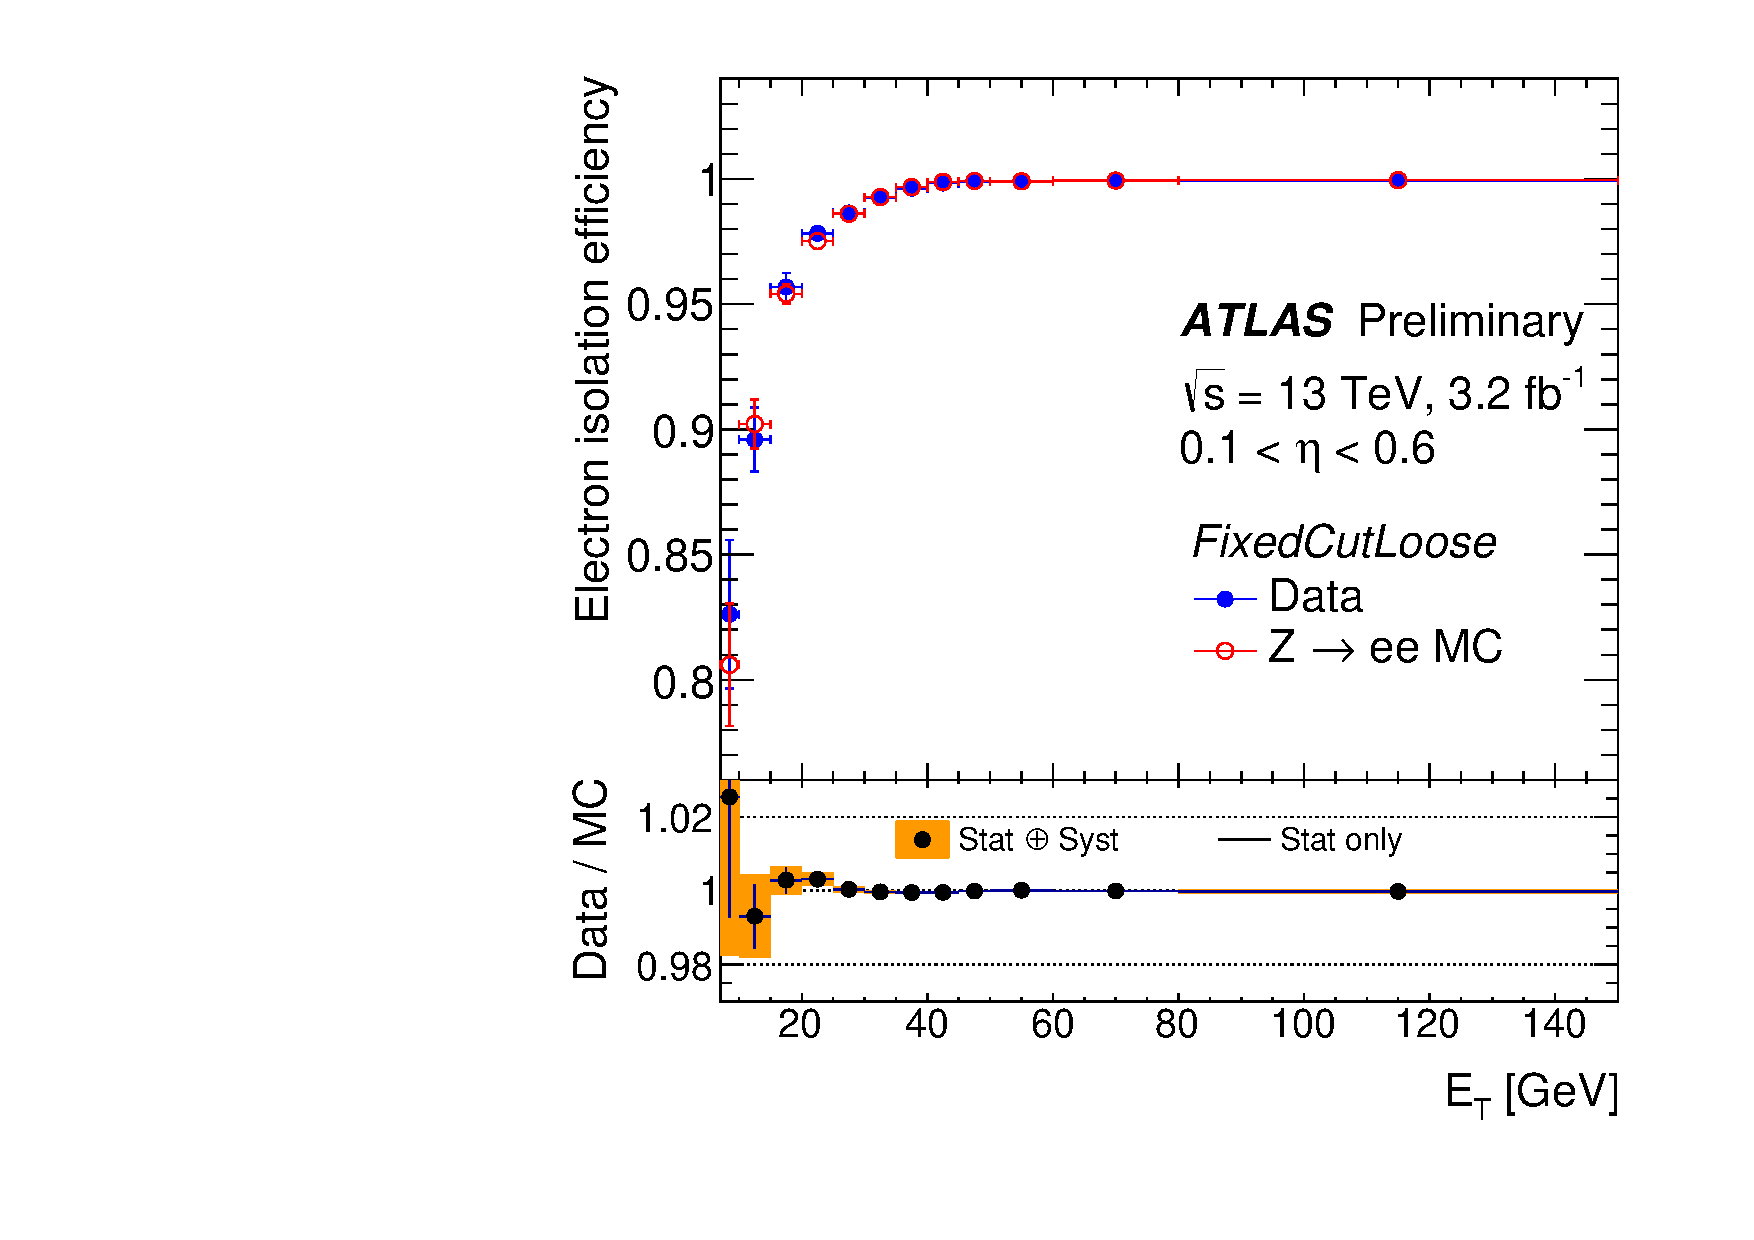
\includegraphics[scale=0.35]{fig_16a.pdf}
            \caption{The transverse energy $E_\mathrm{T}$}
        \end{center}
    \end{subfigure}
    \begin{subfigure}[b]{0.48\textwidth}
        \begin{center}
            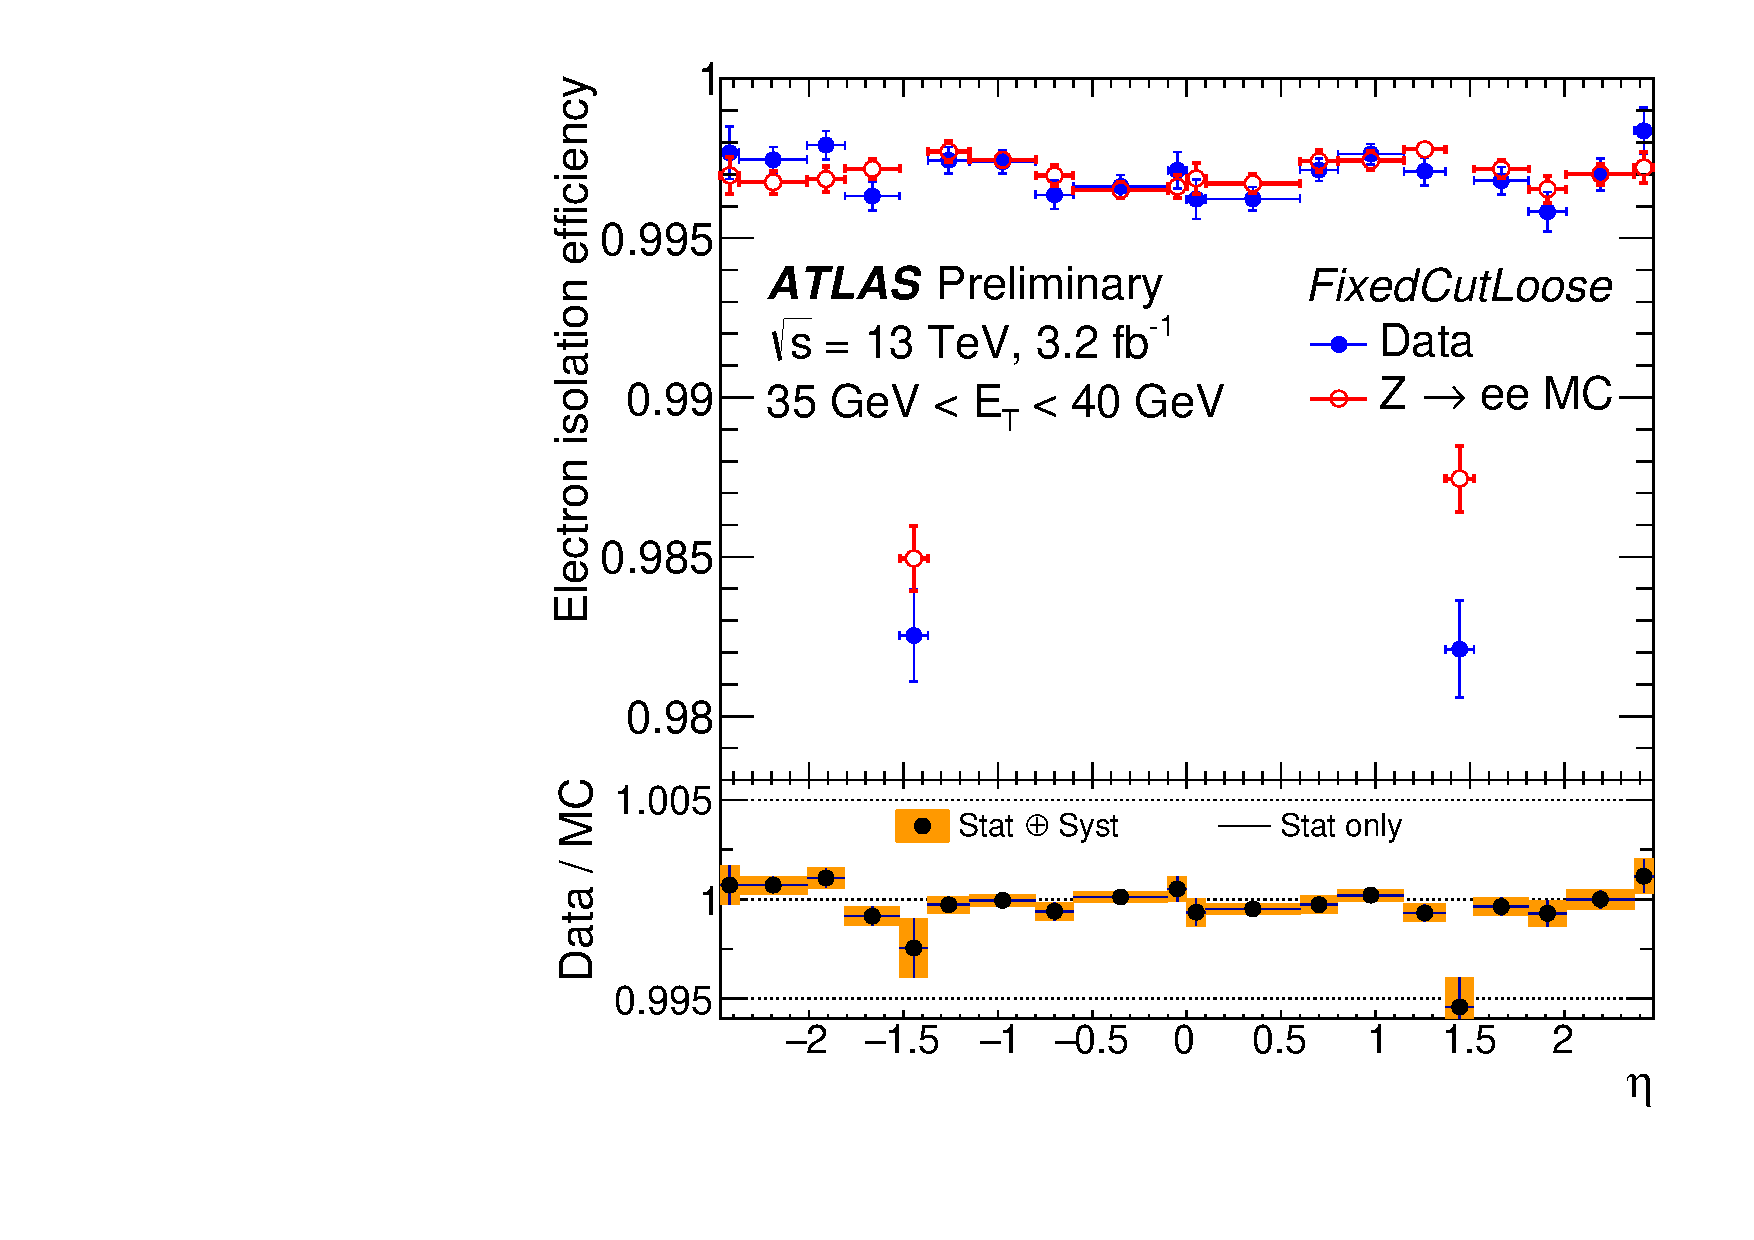
\includegraphics[scale=0.35]{fig_16b.pdf}
            \caption{$\eta$}
        \end{center}
    \end{subfigure}
    \caption{The electron isolation efficiencies for the fixedCutLoose working point for electrons from $Z \to ee$ as a function of the (a) the transverse energy $E_\mathrm{T}$ for $0.1 < \eta < 0.6$ and (b) pseudorapidity $\eta$ for $35 < E_\mathrm{T} < 40$~{\GeV}~\cite{ATLAS:2016iqc}.
    The electrons are required to fulfill \texttt{TightLLH} identification.}
    \label{fig:app_electron_isolation_isolation_plots}
\end{figure}


\chapter{Real lepton efficiency}
\label{app:rle}
\graphicspath{figures/rle}
This appendix presents more details on the measurement of the data-driven real lepton efficiency using the $Z$ tag-and-probe method.

%%%
%%%
%%%

\section{The $Z$ tag-and-probe method}
\label{sec:app_RLE_ZTandP_method}
The $Z$ tag-and-probe method is used to extract the leptons from data and measure the real lepton efficiency.
The selected events are required to have at least two baseline leptons.
The lepton candidates with $\pt > 25$~{\GeV} and satisfying all the signal lepton requirements are categorized into \textit{tag leptons}.
The lepton candidates passing baseline lepton requirements can be classified as \textit{probe leptons}.
In order to form a tag-and-probe pair, the two selected leptons have to carry the same flavor and opposite charge.
The invariant mass of the tag-and-probe pair system should satisfy the $Z$ boson mass window $80 < m_{\ell \ell} < 100$~{\GeV}.
All possible combinations of the tag-and-probe pairs are considered to avoid any bias and to increase the statistics.
For the $Z \to ee$ decay, an additional $|\eta| < 2$ requirement is applied on the tag and probe leptons.
However, no additional requirement is applied for the $Z \to \mu \mu$ decay.
The tag lepton is used to select the probe lepton only and the probe lepton is used for the real efficiency measurements.
In this study, the tag and probe leptons are required to match the lepton triggers listed in Table~\ref{tab:app_RLE_single_lepton_triggers}.

\begin{table}[htb]
    %\begin{center}
    \resizebox{\textwidth}{!}{% <------ Don't forget this %
        \begin{tabular}{cccc}
            \hline
            \hline
            Trigger                                & lepton   & 2015                                     & 2016\\
            \hline
            \multirow{2}{*}{Single lepton trigger} & electron & \texttt{e24\_lhmedium\_iloose\_L1EM20VH} & \texttt{e26\_lhtight\_nod0\_ivarloose}\\
                                                   & muon     & \texttt{mu20\_iloose\_L1MU15}            & \texttt{mu26\_ivarmedium}\\
            \hline
            \multirow{2}{*}{Dilepton trigger}      & electron & \texttt{2e12\_lhloose\_L12EM10VH}        & \texttt{2e17\_lhvloose\_nod0}\\
                                                   & muon     & \texttt{mu18\_mu8noL1}                   & \texttt{mu22\_mu8noL1}\\
            \hline
            \hline
        \end{tabular}
    }
    %\end{center}
    \caption{The list of single lepton and dilepton triggers used for the real lepton efficiency measurements.
    The dilepton triggers are used for studying the systematic uncertainties causing by the trigger.}
    \label{tab:app_RLE_single_lepton_triggers}
\end{table}

Figure~\ref{fig:app_RLE_mll_distributions} shows the data-to-MC comparison of the tag-and-probe pair invariant mass distributions which indicate the need of subtracting the background especially for the probe electron with $\pt < 20$~{\GeV}.
%
\begin{figure}[htb]
    \begin{center}
        \begin{subfigure}[b]{0.48\textwidth}
            \begin{center}
                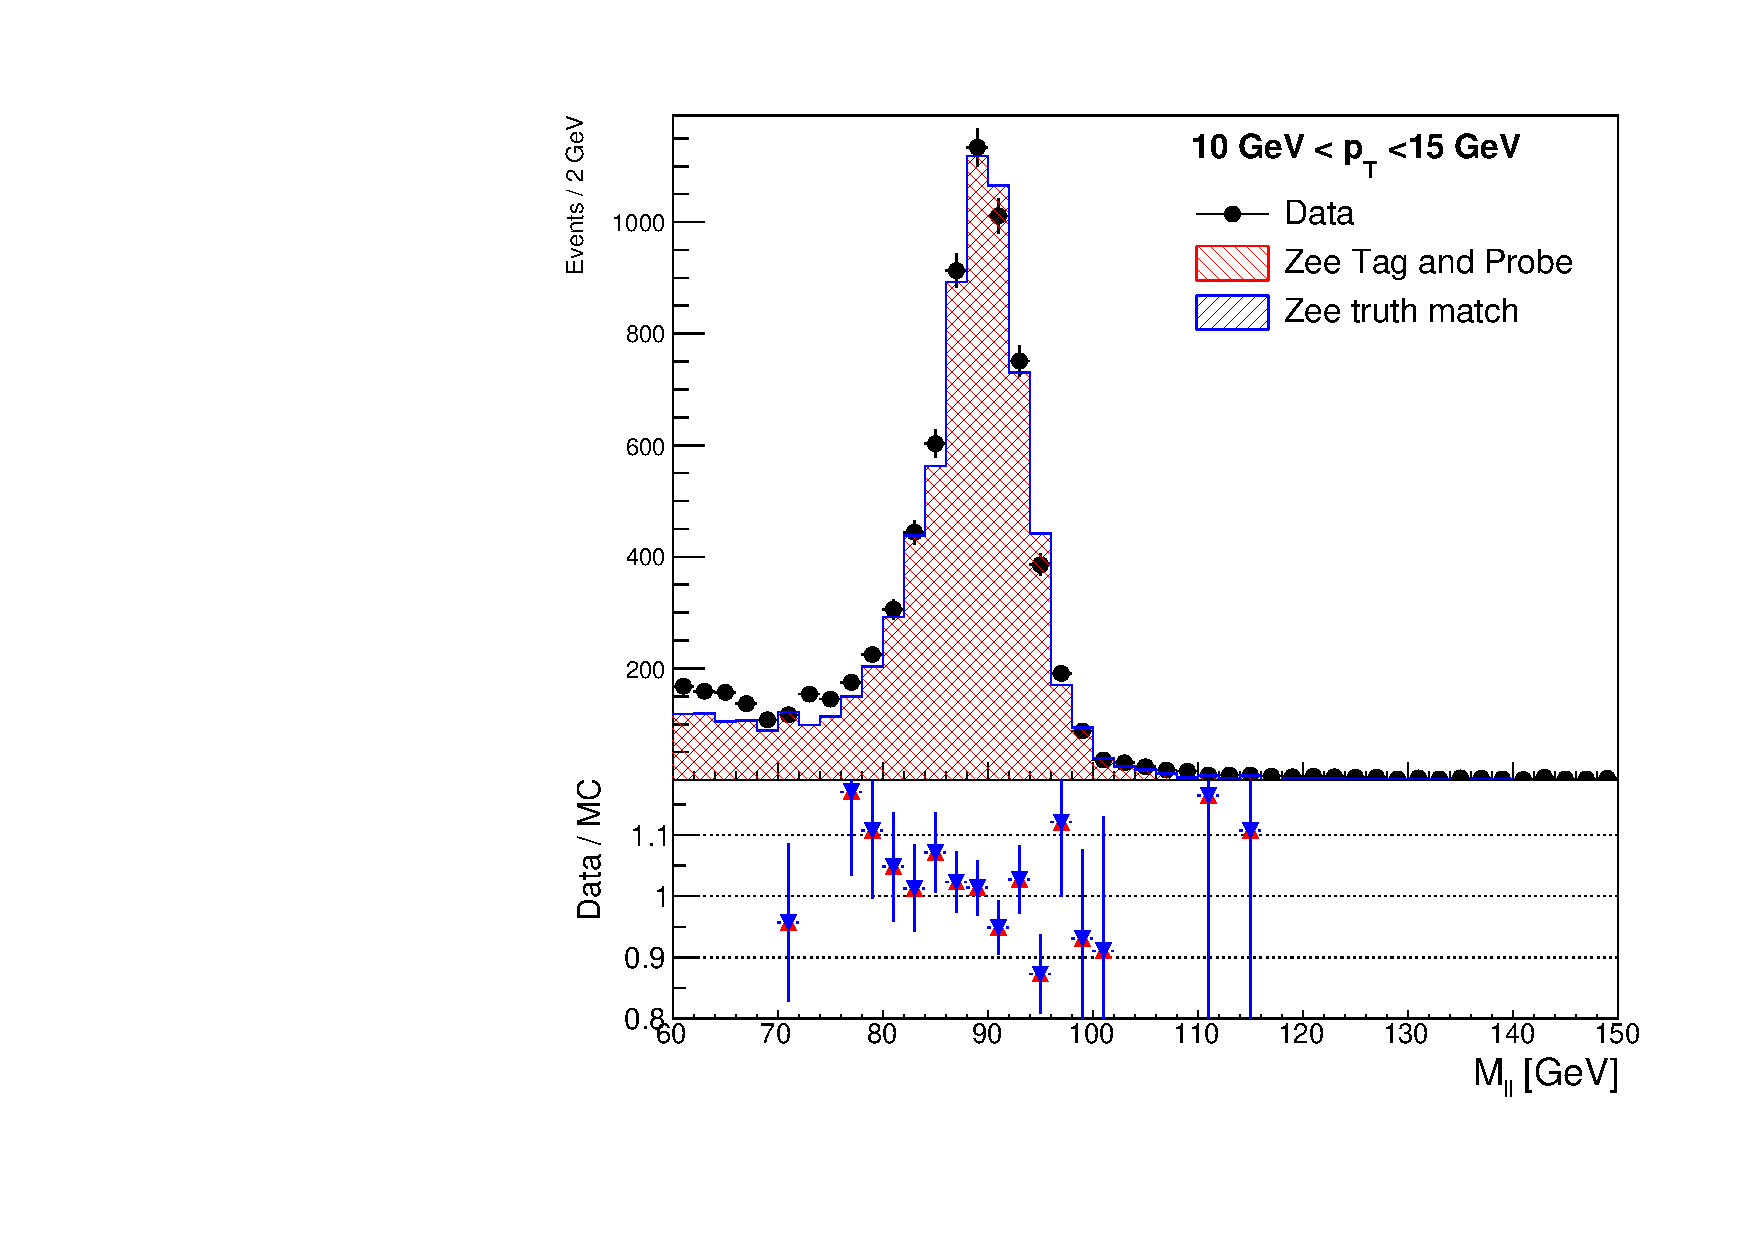
\includegraphics[scale=0.4]{signal_level_Mee_pt1015_ratio_plot_MC_normalized.pdf}
                \caption{The $m_{ee}$ distribution with $10 < \pt < 15$~{\GeV}.}
            \end{center}
        \end{subfigure}%
        \begin{subfigure}[b]{0.48\textwidth}
            \begin{center}
                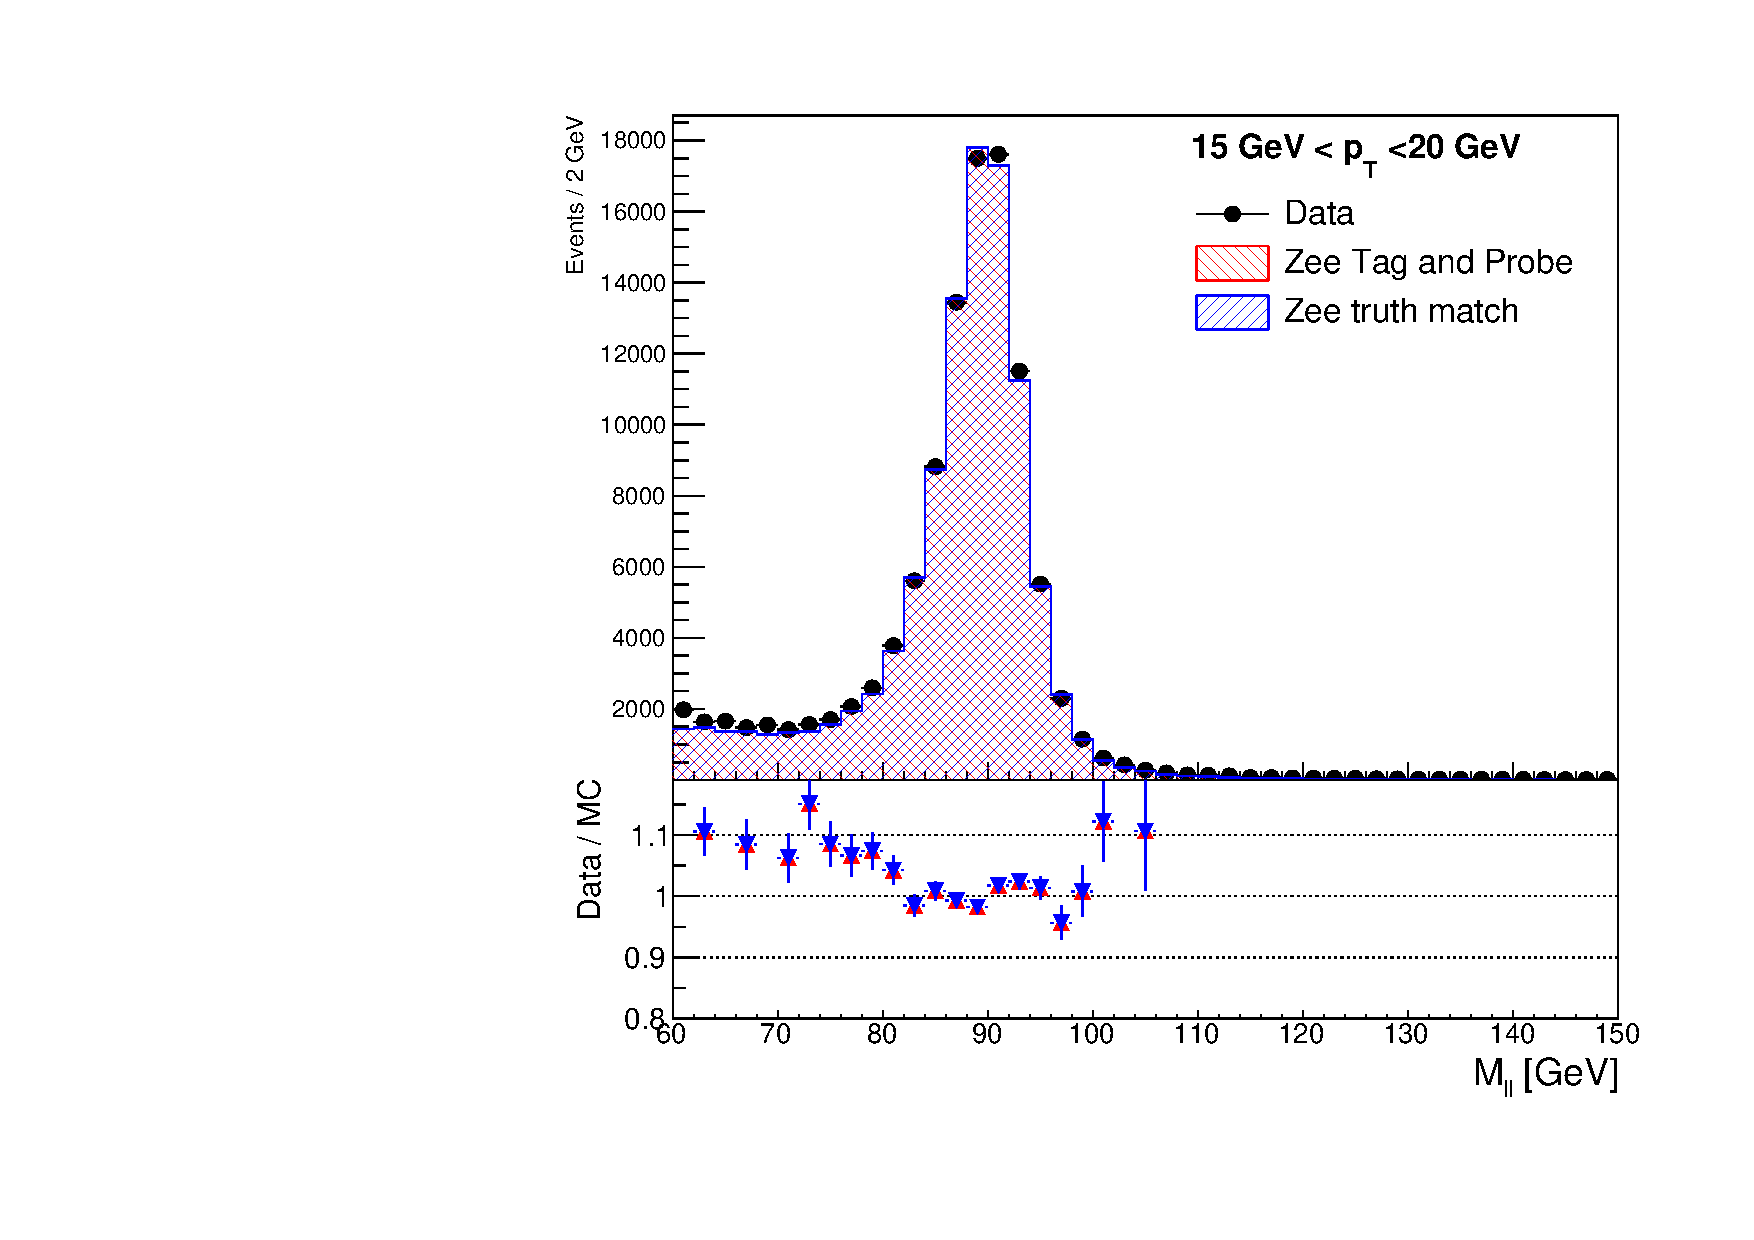
\includegraphics[scale=0.4]{signal_level_Mee_pt1520_ratio_plot_MC_normalized.pdf}
                \caption{The $m_{ee}$ distribution with $15 < \pt < 20$~{\GeV}.}
            \end{center}
        \end{subfigure}
        \begin{subfigure}[b]{0.48\textwidth}
            \begin{center}
                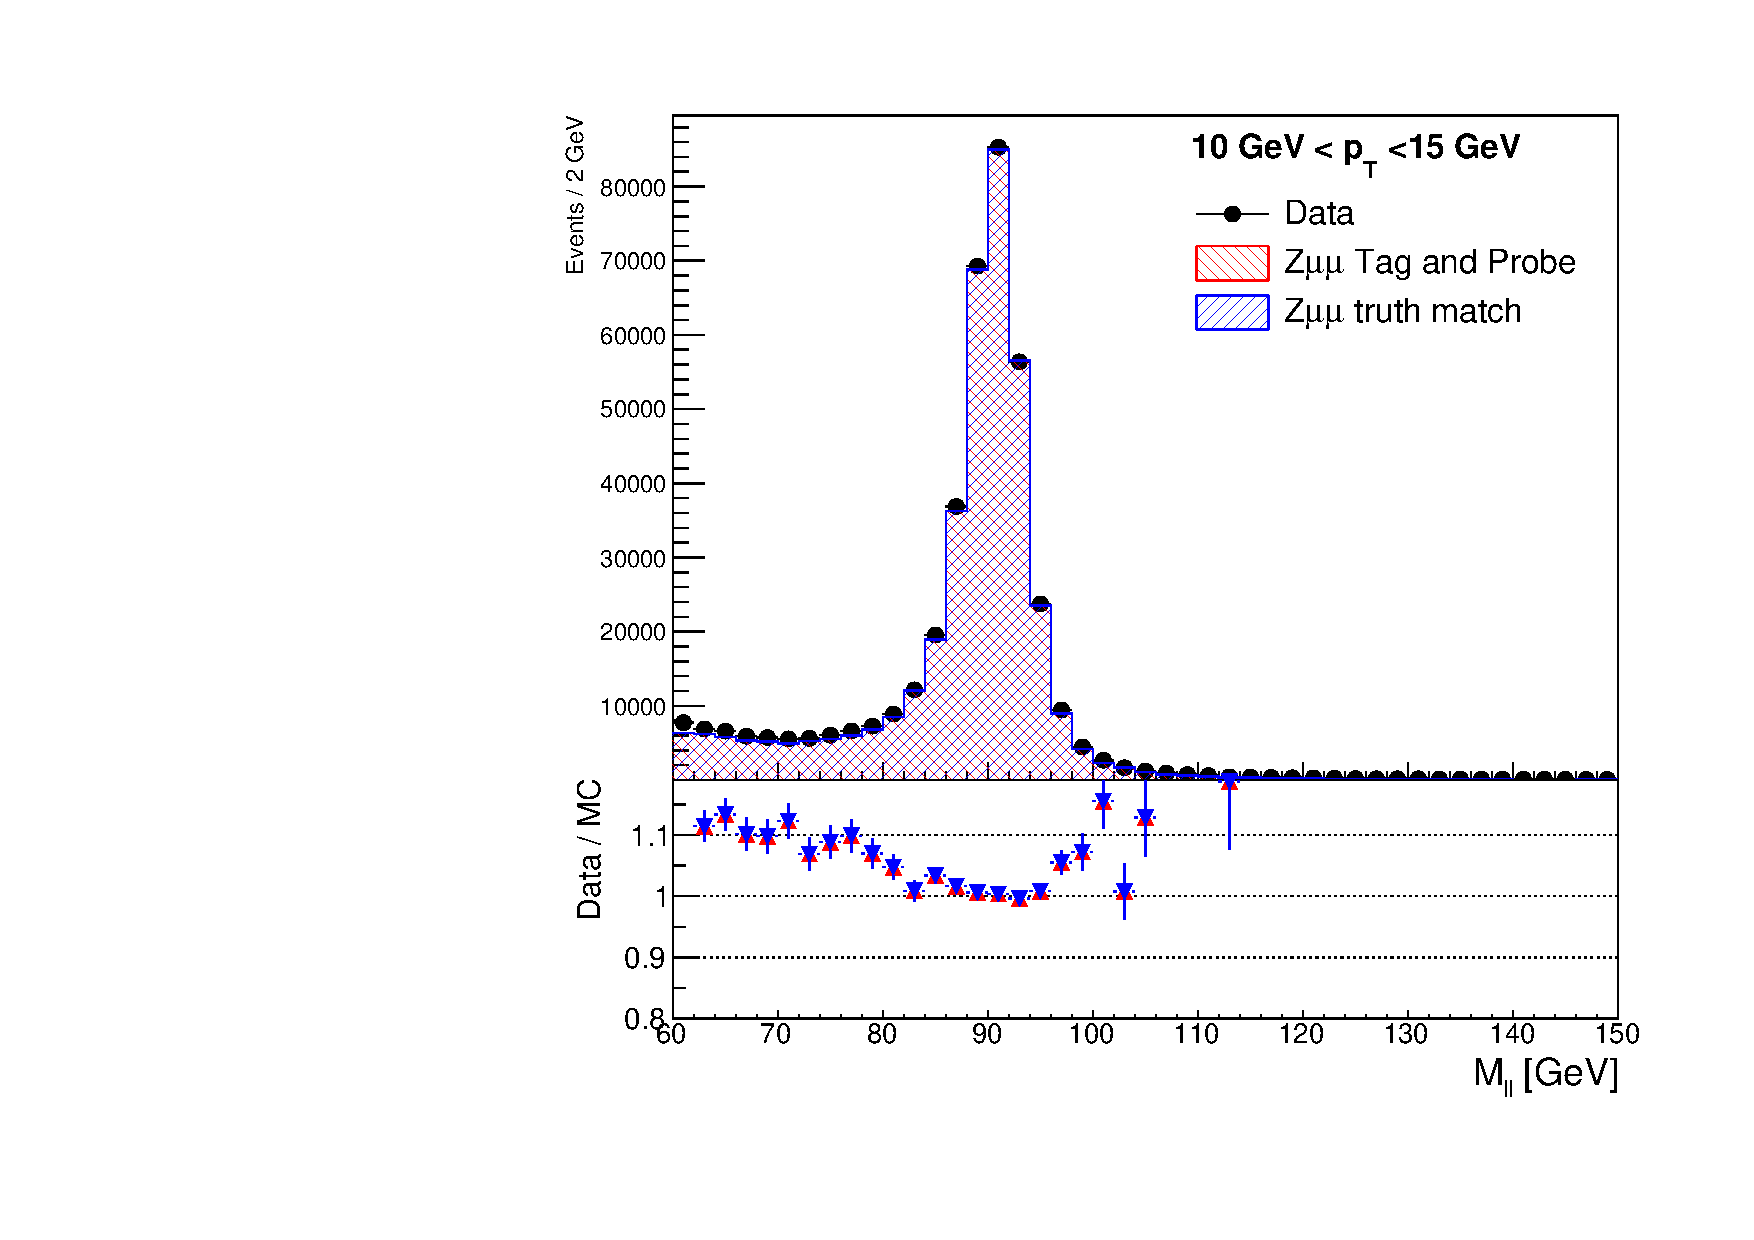
\includegraphics[scale=0.4]{signal_level_Mmumu_pt1015_ratio_plot_MC_normalized.pdf}
                \caption{The $m_{\mu\mu}$ distribution with $10 < \pt < 15$~{\GeV}.}
            \end{center}
        \end{subfigure}%
        \begin{subfigure}[b]{0.48\textwidth}
            \begin{center}
                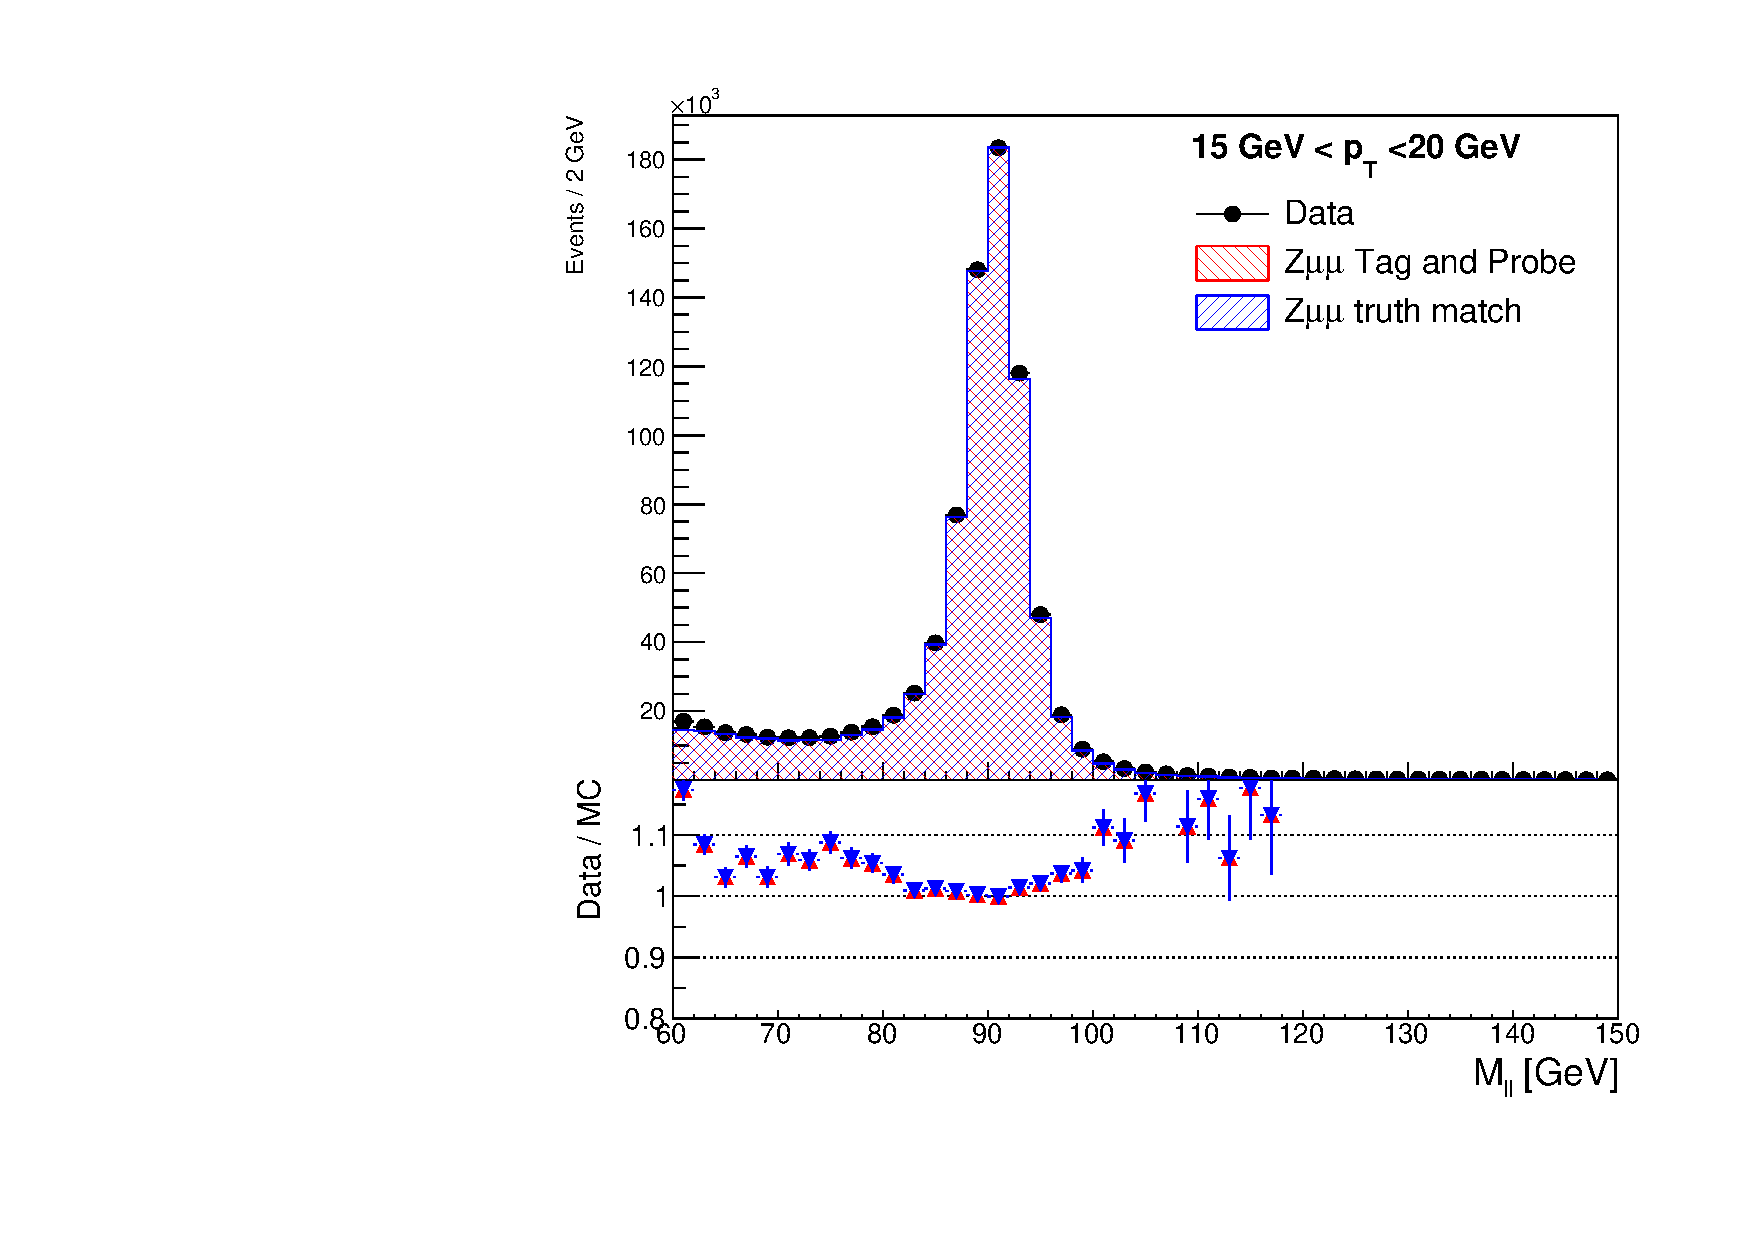
\includegraphics[scale=0.4]{signal_level_Mmumu_pt1520_ratio_plot_MC_normalized.pdf}
                \caption{The $m_{\mu\mu}$ distribution with $15 < \pt < 20$~{\GeV}.}
            \end{center}
        \end{subfigure}
    \end{center}
    \caption{The invariant mass distributions of the tag-and-probe pair computed using $Z+jets$ MC and 2015 + 2016 data.
    The red color stands for the $Z$ tag-and-probe events, the blue color represents the $Z$ truth matched events, and the black dots are data.
    The MC distributions are scaled to the data using a Gaussian fit of the $Z$ mass peak $85 < m_{\ell \ell} < 95$~{\GeV}.}
    \label{fig:app_RLE_mll_distributions}
\end{figure}
%
A background template method, which is similar to the one used by the $e/\gamma$ performance group for their efficiency measurements~\cite{ATLAS-CONF-2014-018}, is used to estimate the background contamination from the low \pt electrons.
No background subtraction is performed on the signal leptons because the background contamination is found to be negligible.
However, the background contamination in the baseline probe leptons needs to be subtracted.
The real lepton efficiency is obtained by the following equation
%
\begin{equation}
    \epsilon = \frac{N_{\mathrm{signal}}}{N_{\mathrm{baseline}} - N_{\mathrm{baseline}}^{bkg}}
    \label{eq:app_RLE_efficiency_formula}
\end{equation}
%
where $N_\mathrm{signal}$ is the number of probe leptons passing the signal requirements, $N_\mathrm{baseline}$ is the number of probe leptons passing the baseline requirements, and $N_\mathrm{baseline}^{bkg}$ is the estimated background contamination in the baseline probe leptons.

%%%
%%%
%%%

\section{Background subtraction}
\label{sec:app_RLE_bkg_subtraction}
The background template method is used to evaluate the background contamination on data.
By inverting the calorimeter and track isolations, requesting the electron object to fail the medium LH identification, the background sample enriched template can be obtained.
Three background templates are considered for the systematic study.
The definitions of the background template are summarized in Table~\ref{tab:app_RLE_bkg_templates}.
%
\begin{table}[htbp]
    %\begin{center}
    \resizebox{\textwidth}{!}{% <------ Don't forget this %
        \begin{tabular}{cccc}
            \hline
            \hline
            cut                   & variation 1 template                   & baseline template                       & variation 2 template\\
            \hline
            Identification        & -                                      & fail medium LH                          & fail medium LH\\
            Calorimeter isolation & $E_\mathrm{T}^{topocone20} /\pt > 6\%$ & $E_\mathrm{T}^{topocone20} /\pt > 15\%$ & $E_\mathrm{T}^{topocone20} /\pt > 20\%$\\
            Track isolation       & $p_\mathrm{T}^{varcone20} /\pt > 6\%$  & $E_\mathrm{T}^{topocone20} /\pt > 8\%$  & $E_\mathrm{T}^{topocone20} /\pt > 15\%$\\
            \hline
            \hline
        \end{tabular}
    }
    %\end{center}
    \caption{The definition of the background templates for estimating the background contamination associated with the $Z$ tag-and-probe method.
    The baseline template is used to estimate the background contamination.
    The variation 1 template has looser requirements and the variation 2 template has tighter requirements.
    They are used to assess the systematic caused by the background contamination.}
    \label{tab:app_RLE_bkg_templates}
\end{table}
%
Figure~\ref{fig:app_RLE_bkg_templates} shows the $m_{ee}$ distributions of the background template.
%
\begin{figure}[htbp]
    \begin{subfigure}[b]{0.48\textwidth}
        \begin{center}
            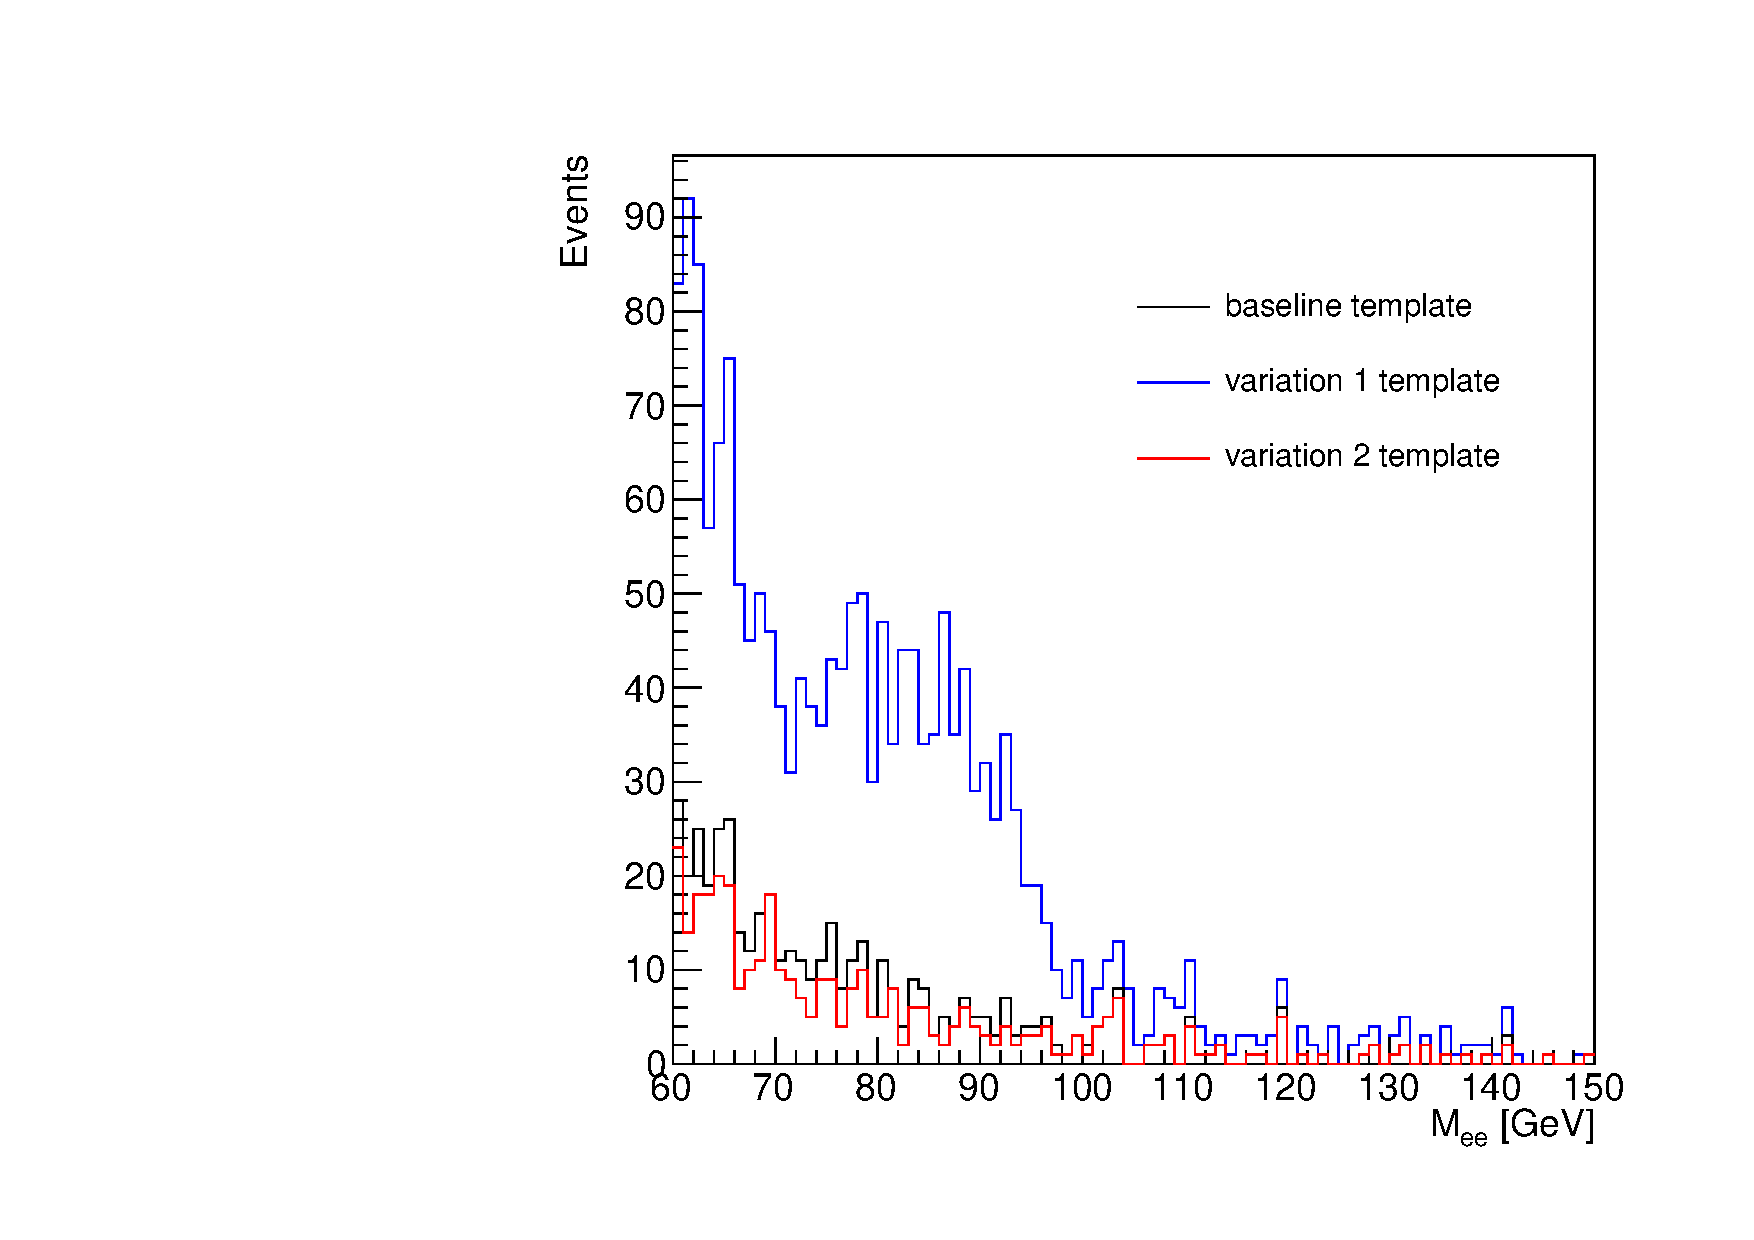
\includegraphics[scale=0.4]{bkg_template_electron_pt_1015_eta0201.pdf}
            \caption{Probe electrons with $10 < \pt < 15$~{\GeV}.}
        \end{center}
    \end{subfigure}
    \begin{subfigure}[b]{0.48\textwidth}
        \begin{center}
            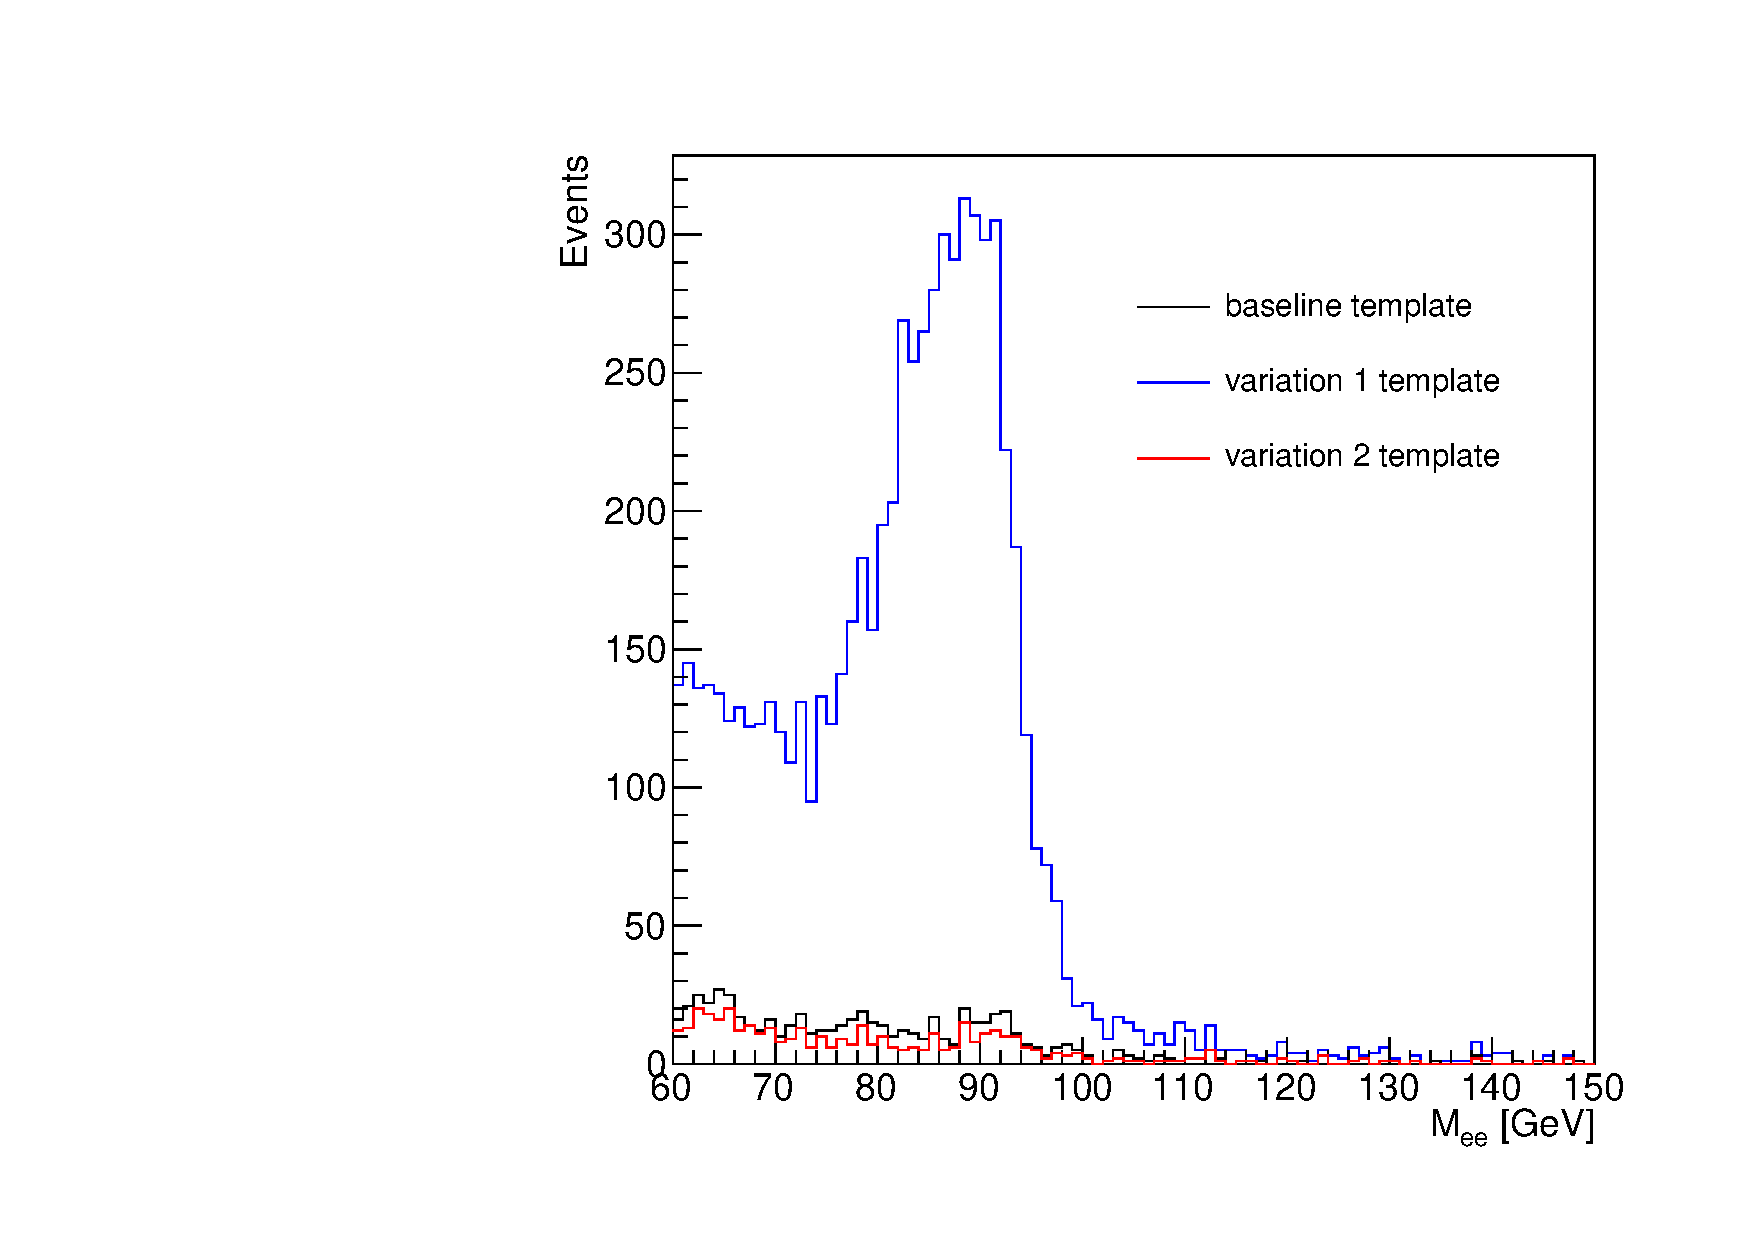
\includegraphics[scale=0.4]{bkg_template_electron_pt_1520_eta0201.pdf}
            \caption{Probe electrons with $15 < \pt < 20$~{\GeV}.}
        \end{center}
    \end{subfigure}
    \caption{The $m_{ee}$ distributions for the baseline, variation 1 and variation 2 background templates.
    The $m_{ee}$ distributions are computed using the probe electrons with different \pt as indicated in the caption of plots.
    The variation 1 template has looser calorimeter and track isolation requirements and the baseline and the variation 2 templates have tighter selection criteria.
    So a peak can be seen in the $Z$ mass region in variation 1 template but not in the baseline and variation 2 templates.}
    \label{fig:app_RLE_bkg_templates}
\end{figure}
%
The invariant mass distribution of the template events ($m_{ee}^\mathrm{template}$) is then used to estimate the amount of background in $80 < m_{\ell \ell} < 100$~{\GeV} region.
In order to estimate the correct of background events, the $120 < m_{ee} < 150$~{\GeV} region is used to normalize the background template because a smaller prompt electron contribution is expected in this region.
Equation~\ref{eq:app_RLE_bkg_in_the_tail} shows the estimation of the number of background events in the tail region using the baseline electrons.
%
\begin{equation}
    N_{bkg}^\mathrm{tail} = N_\mathrm{baseline}^\mathrm{tail} - N_\mathrm{MC, prompt}^\mathrm{tail}
    \label{eq:app_RLE_bkg_in_the_tail}
\end{equation}
%
where $N_\mathrm{baseline}^\mathrm{tail}$ can be obtained by integrating the baseline $m_{ee}$ distribution in the tail region and $N_\mathrm{MC, prompt}^\mathrm{tail}$ is the prompt electron contamination which is estimated by integrating the $m_{ee}$ distribution in the tail region using the $Z \to ee$ MC simulation.
Because the baseline electron selection criteria already provides a relatively high purity of prompt electrons, the background template suffers from low statistics in the tail region.
The template is fitted in region $60 < m_{ee}^\mathrm{template} < 120$~{\GeV} using an exponential function to avoid any bias in the normalization factor due to statistical fluctuations.
However, the $80 < m_{ee}^\mathrm{template} < 100$~{\GeV} is excluded to minimize the prompt lepton contamination arising from $Z \to ee$ decays.
The fit is mostly driven by the $60 < m_{ee}^\mathrm{template} < 80$~{\GeV} due to the low statistics in the tail.
After fitting is performed, the template in the tail region $N_\mathrm{template}^\mathrm{tail}$ is normalized to the background in the tail $N_{bkg}^\mathrm{tail}$ to get the correct estimated number of background events.
The baseline $m_{ee}$ distributions before and after applying the background subtraction using the background template are shown in Fig.~\ref{fig:app_RLE_bkg_estimations}.
%
\begin{figure}[htbp]
    \begin{subfigure}[b]{0.32\textwidth}
        \begin{center}
            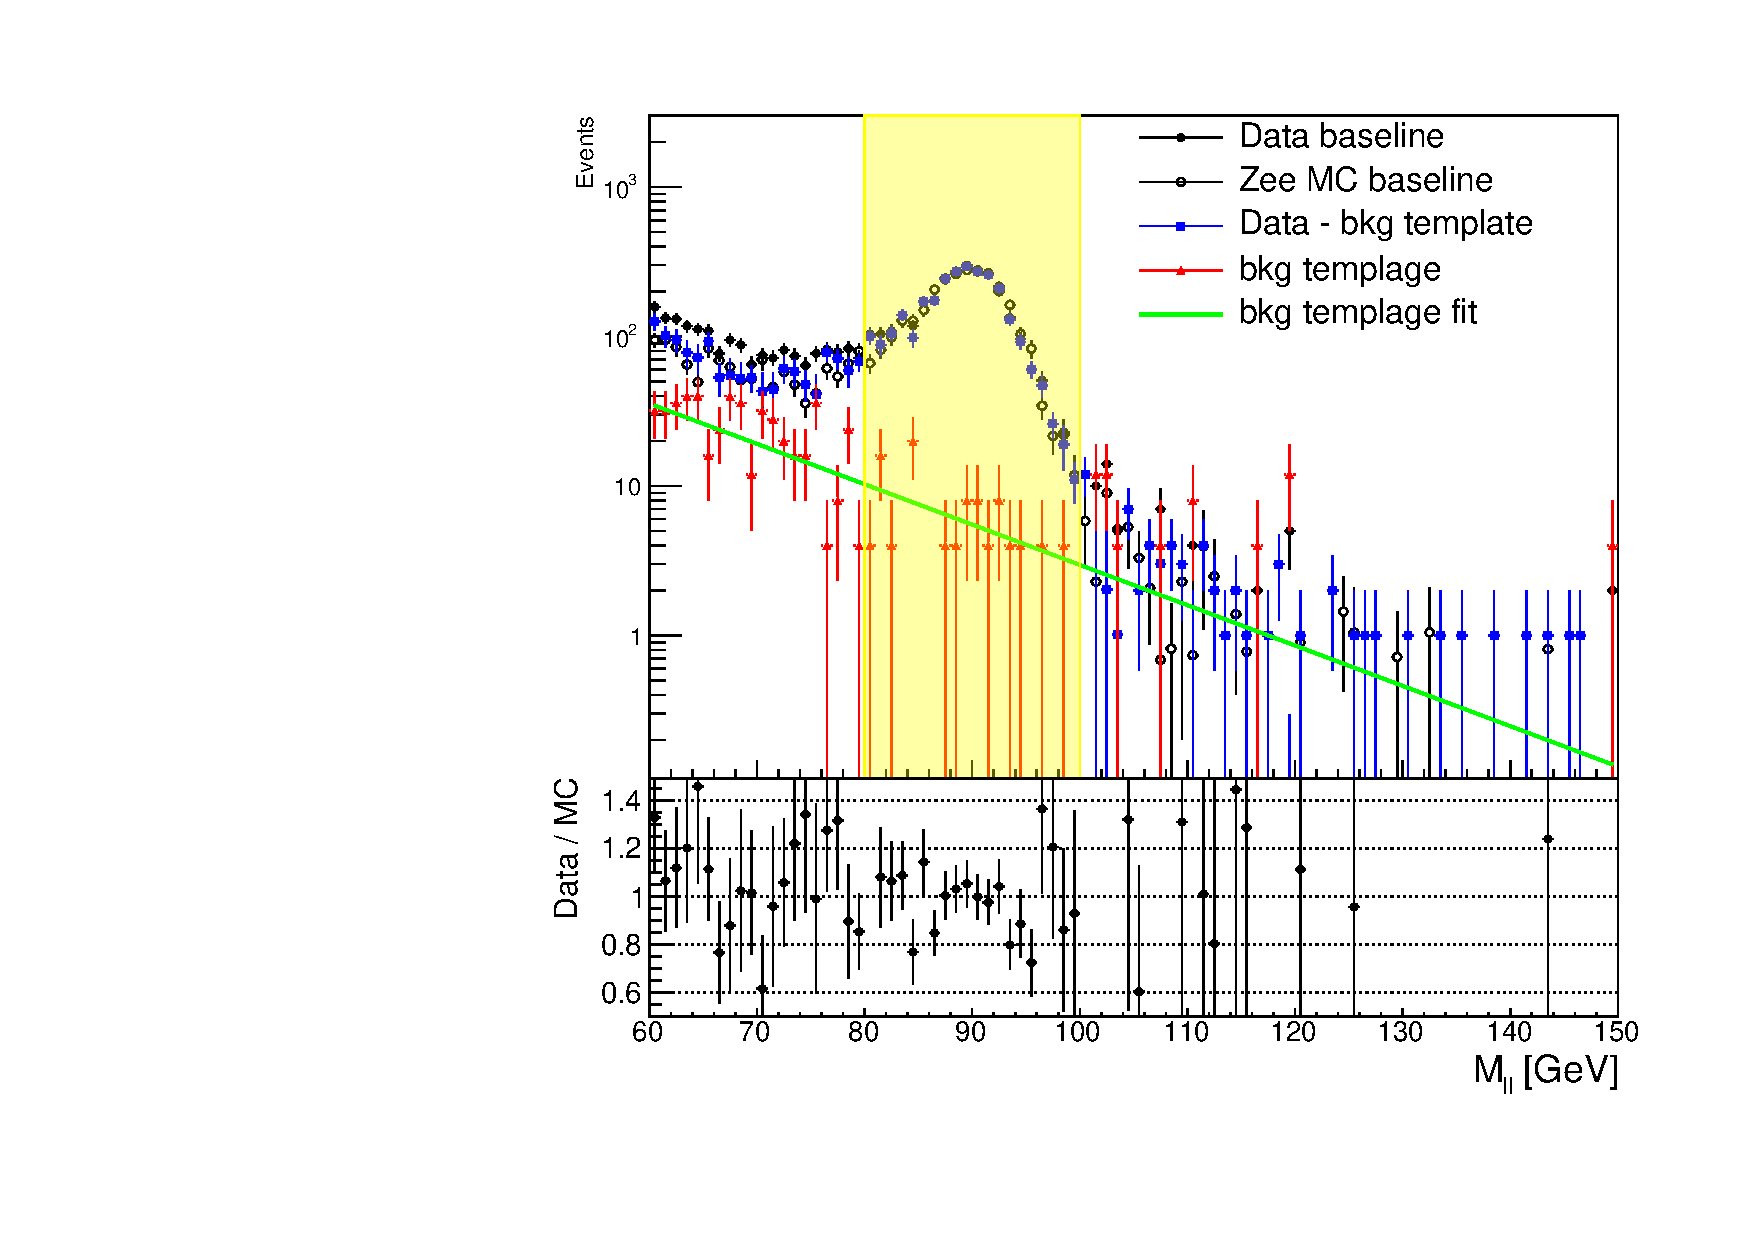
\includegraphics[scale=0.27]{bkg_subtraction_baseline_template_range_baseline_mll80_100_pt10_15_eta0_80_tag_trigger_matched.pdf}
            \caption{$10 < \pt < 15$~{\GeV}\\$0 < |\eta| < 0.8$}
        \end{center}
    \end{subfigure}
    \begin{subfigure}[b]{0.32\textwidth}
        \begin{center}
            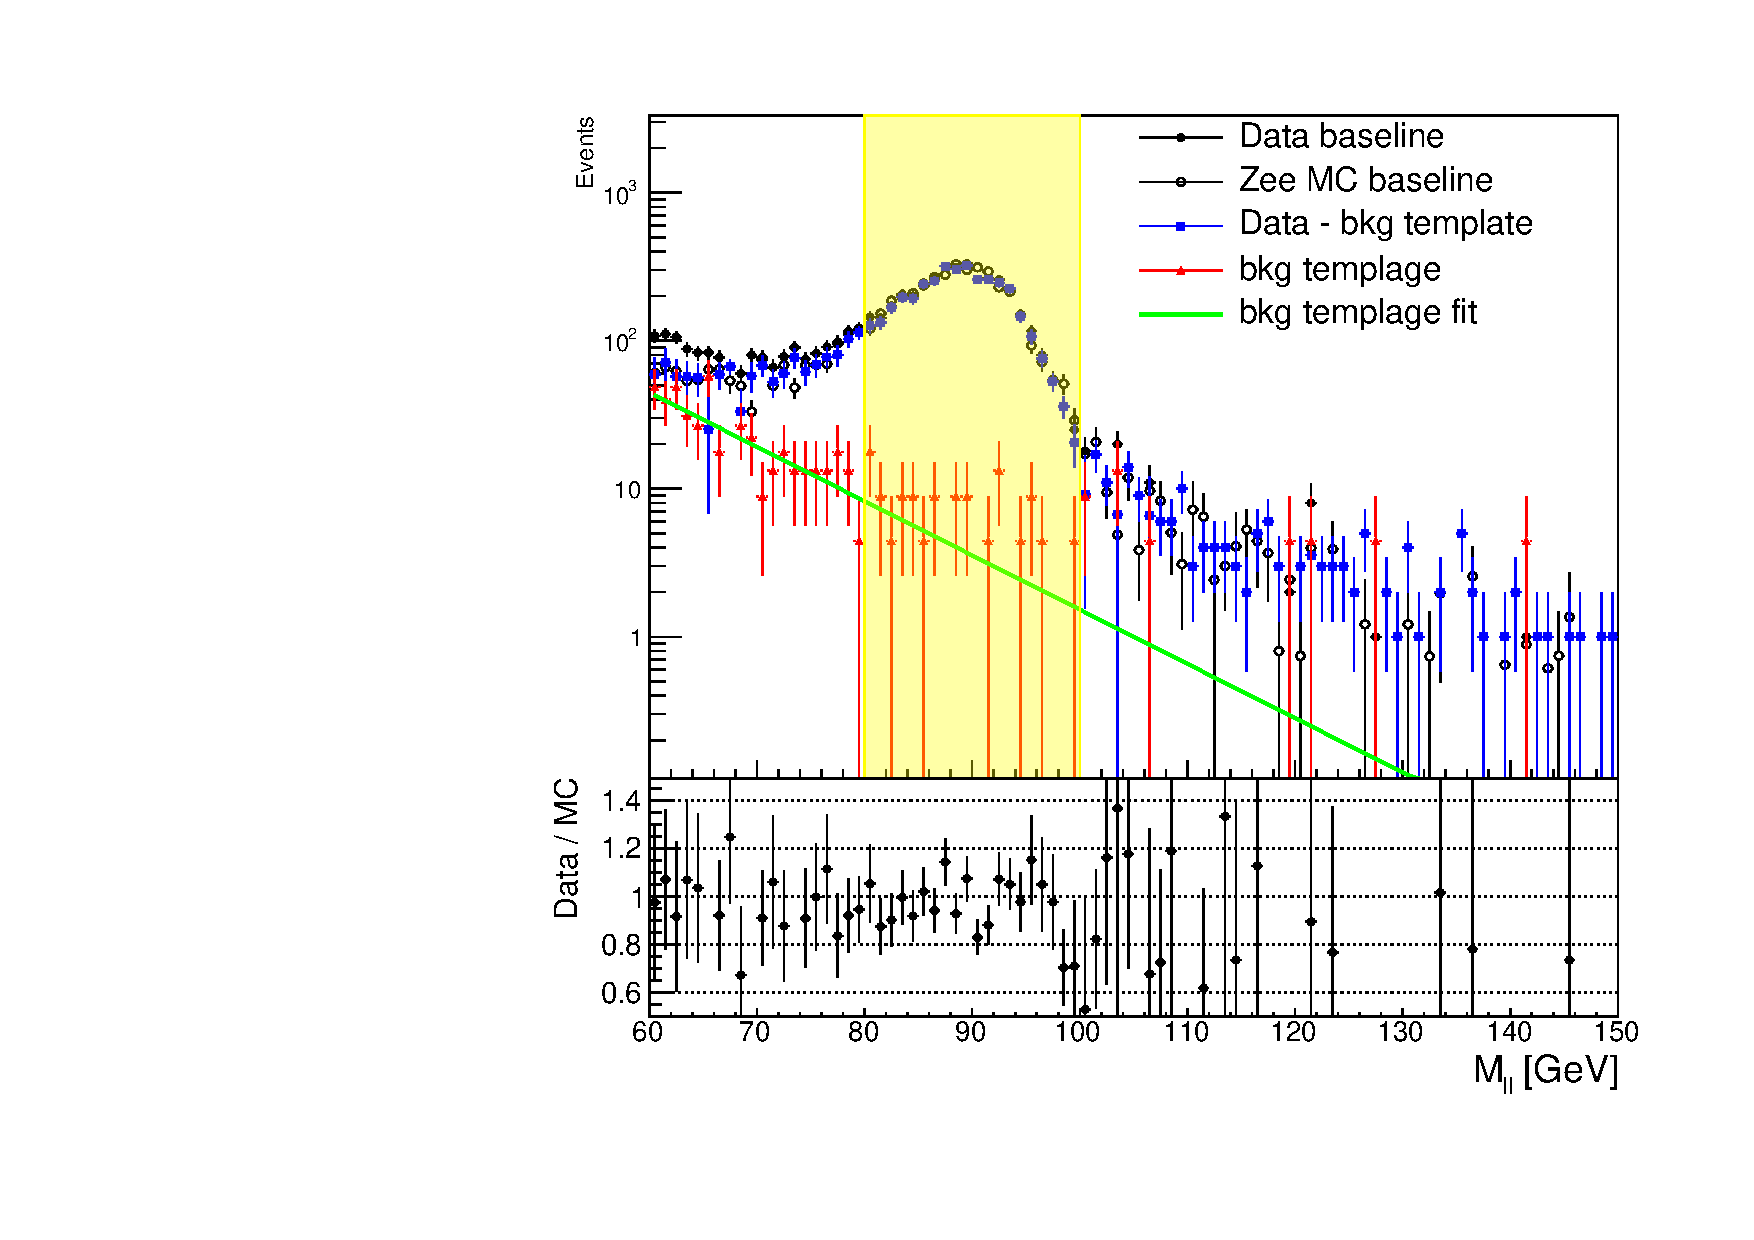
\includegraphics[scale=0.27]{bkg_subtraction_baseline_template_range_baseline_mll80_100_pt10_15_eta80_137_tag_trigger_matched.pdf}
            \caption{$10 < \pt < 15$~{\GeV}\\$0.8 < |\eta| < 1.37$}
        \end{center}
    \end{subfigure}
    \begin{subfigure}[b]{0.32\textwidth}
        \begin{center}
            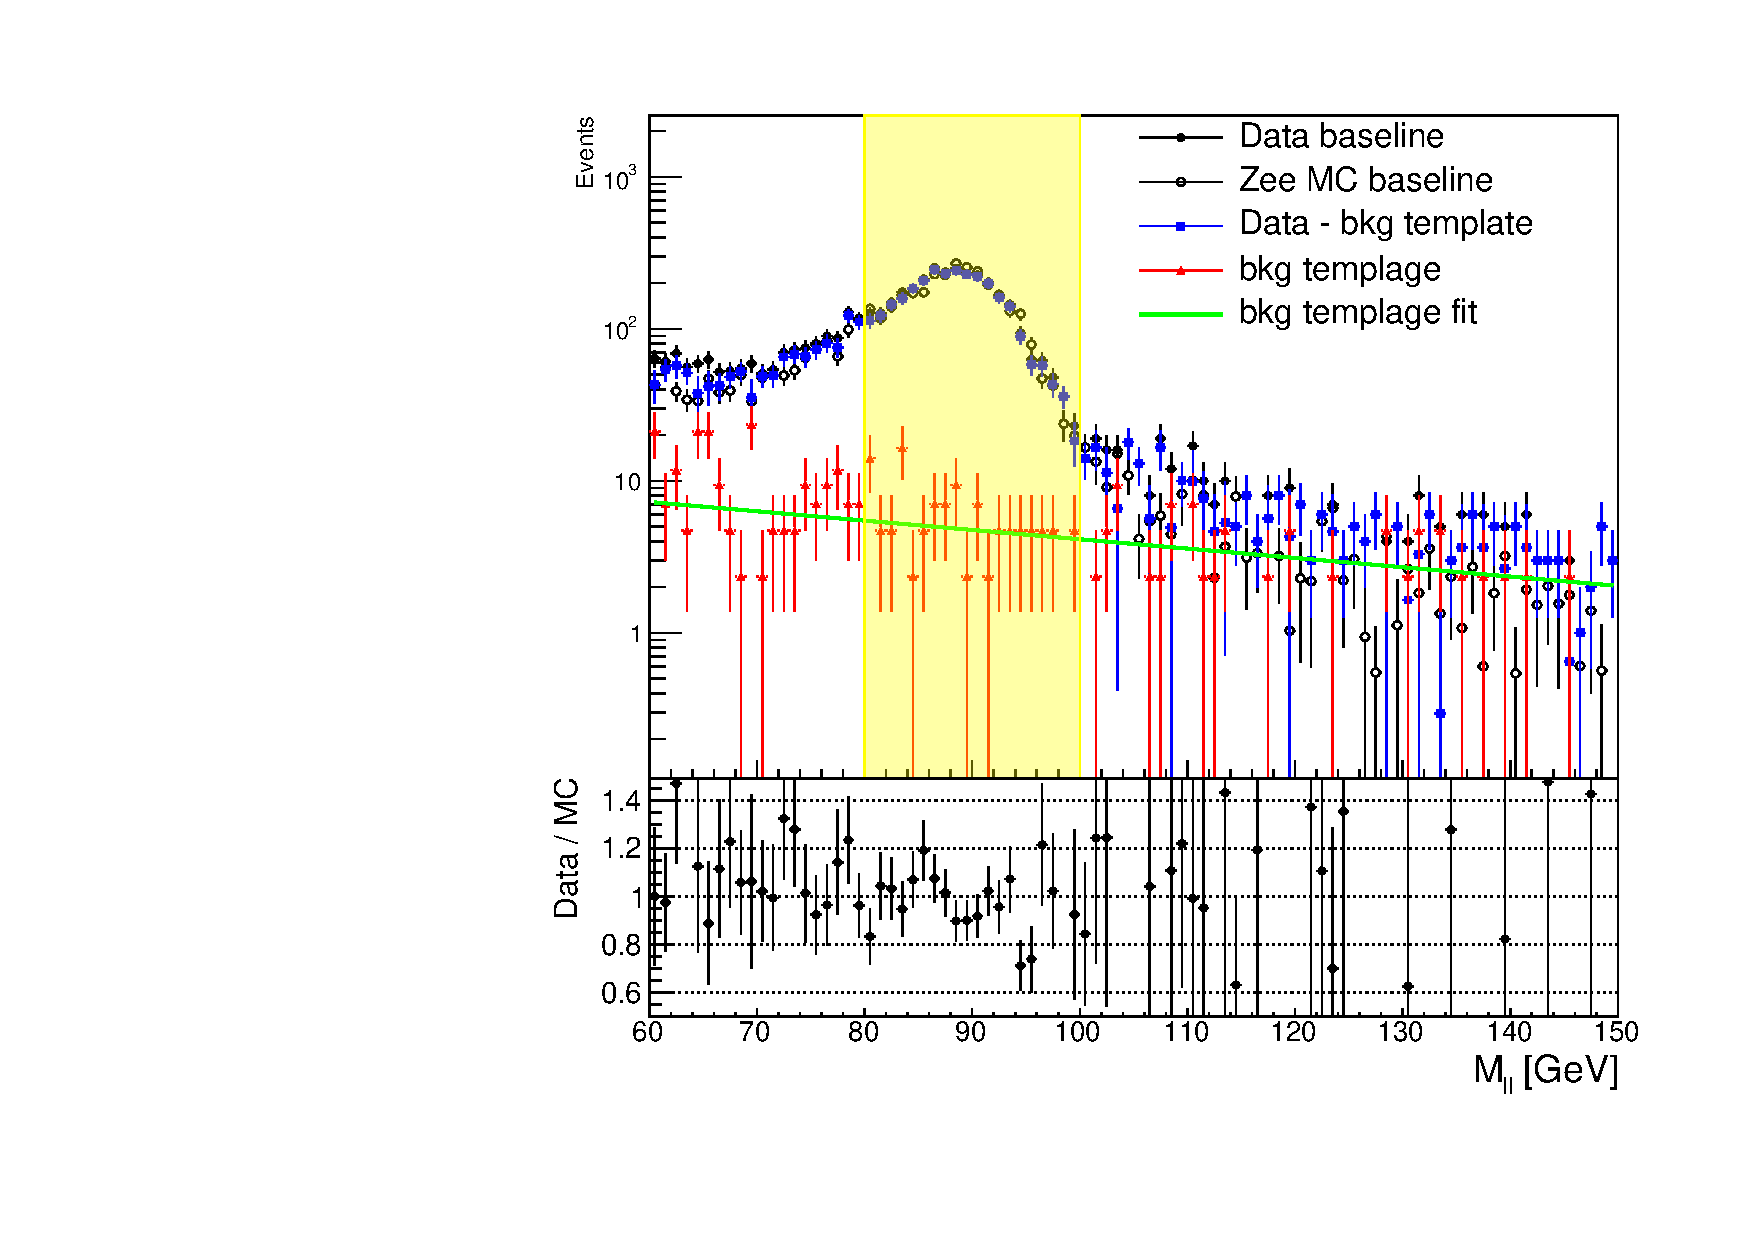
\includegraphics[scale=0.27]{bkg_subtraction_baseline_template_range_baseline_mll80_100_pt10_15_eta151_200_tag_trigger_matched.pdf}
            \caption{$10 < \pt < 15$~{\GeV}\\$1.52 < |\eta| < 2.0$}
        \end{center}
    \end{subfigure}
    \\
    \begin{subfigure}[b]{0.32\textwidth}
        \begin{center}
            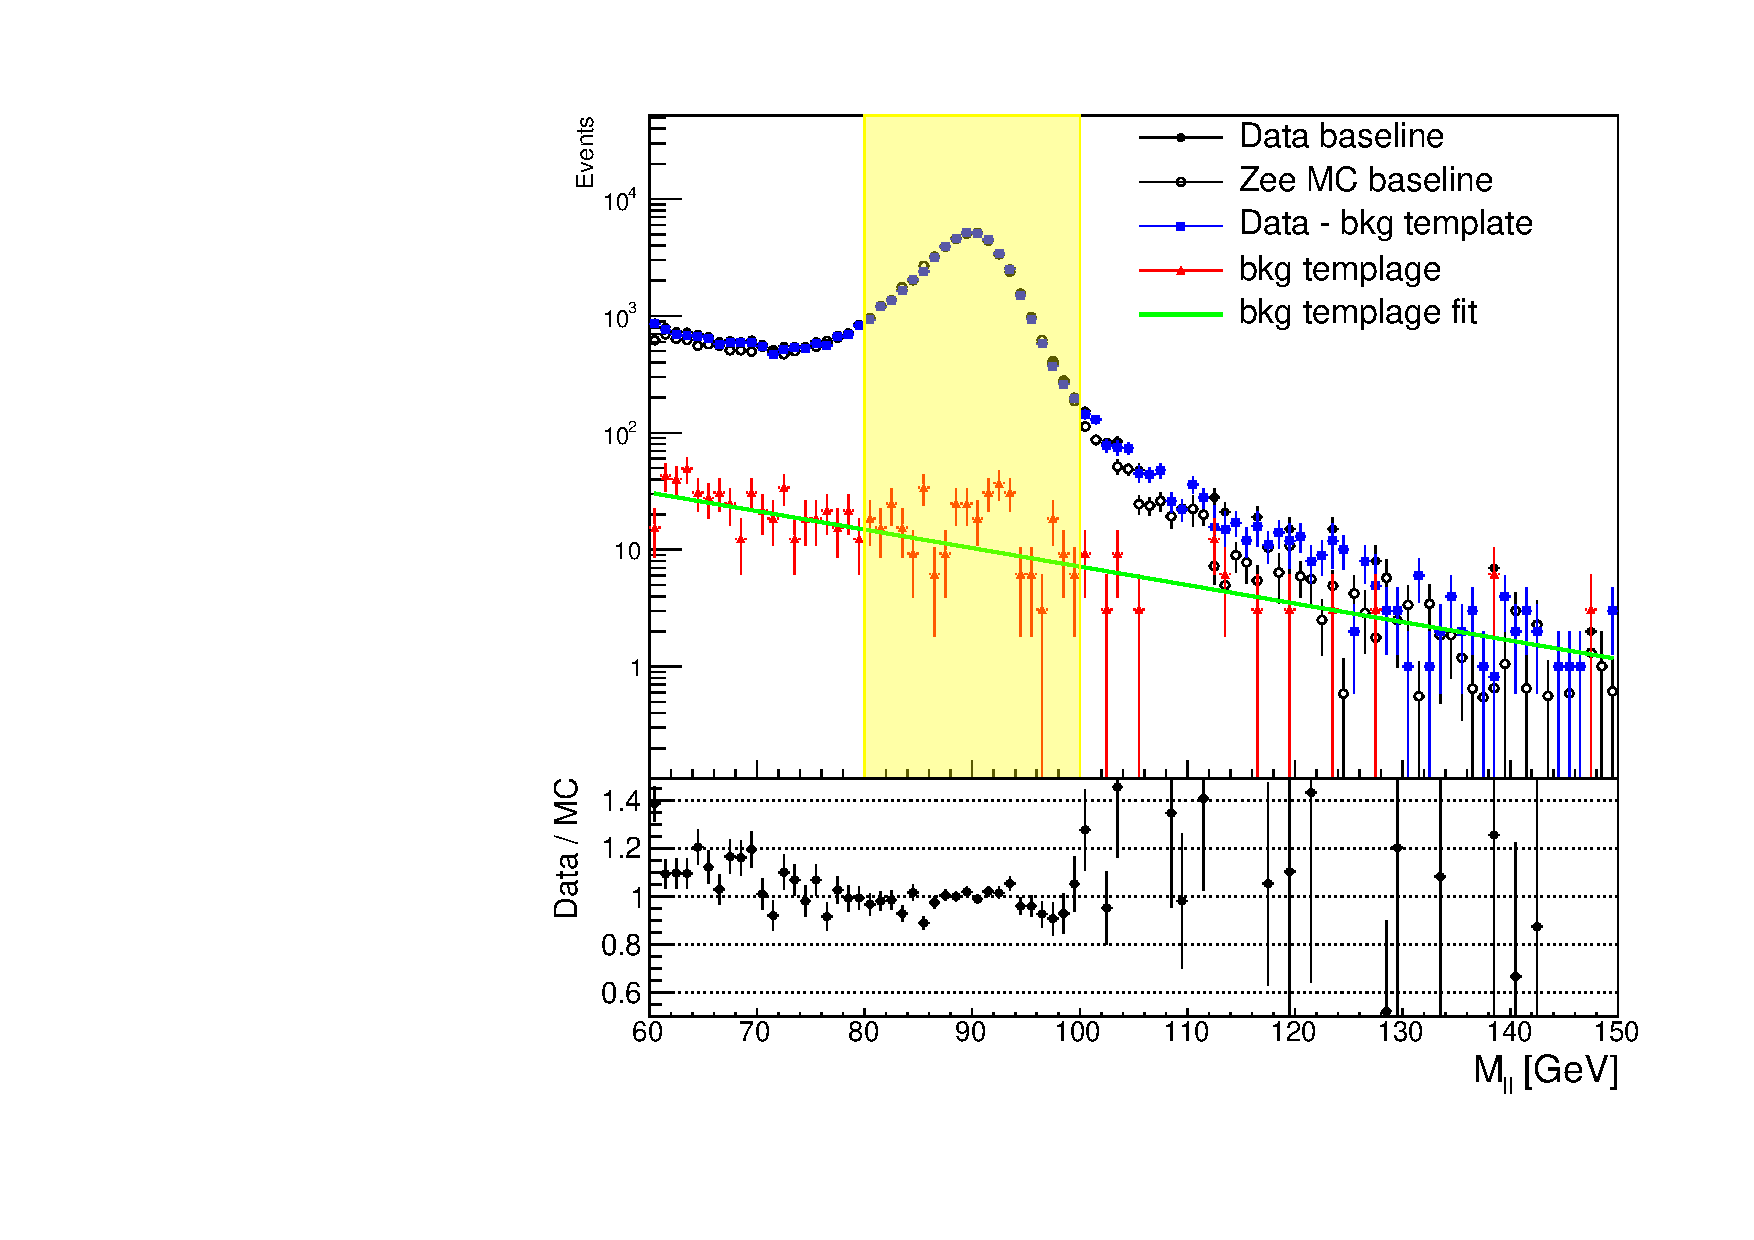
\includegraphics[scale=0.27]{bkg_subtraction_baseline_template_range_baseline_mll80_100_pt15_20_eta0_80_tag_trigger_matched.pdf}
            \caption{$15 < \pt < 20$~{\GeV}\\$0 < |\eta| < 0.8$}
        \end{center}
    \end{subfigure}
    \begin{subfigure}[b]{0.32\textwidth}
        \begin{center}
            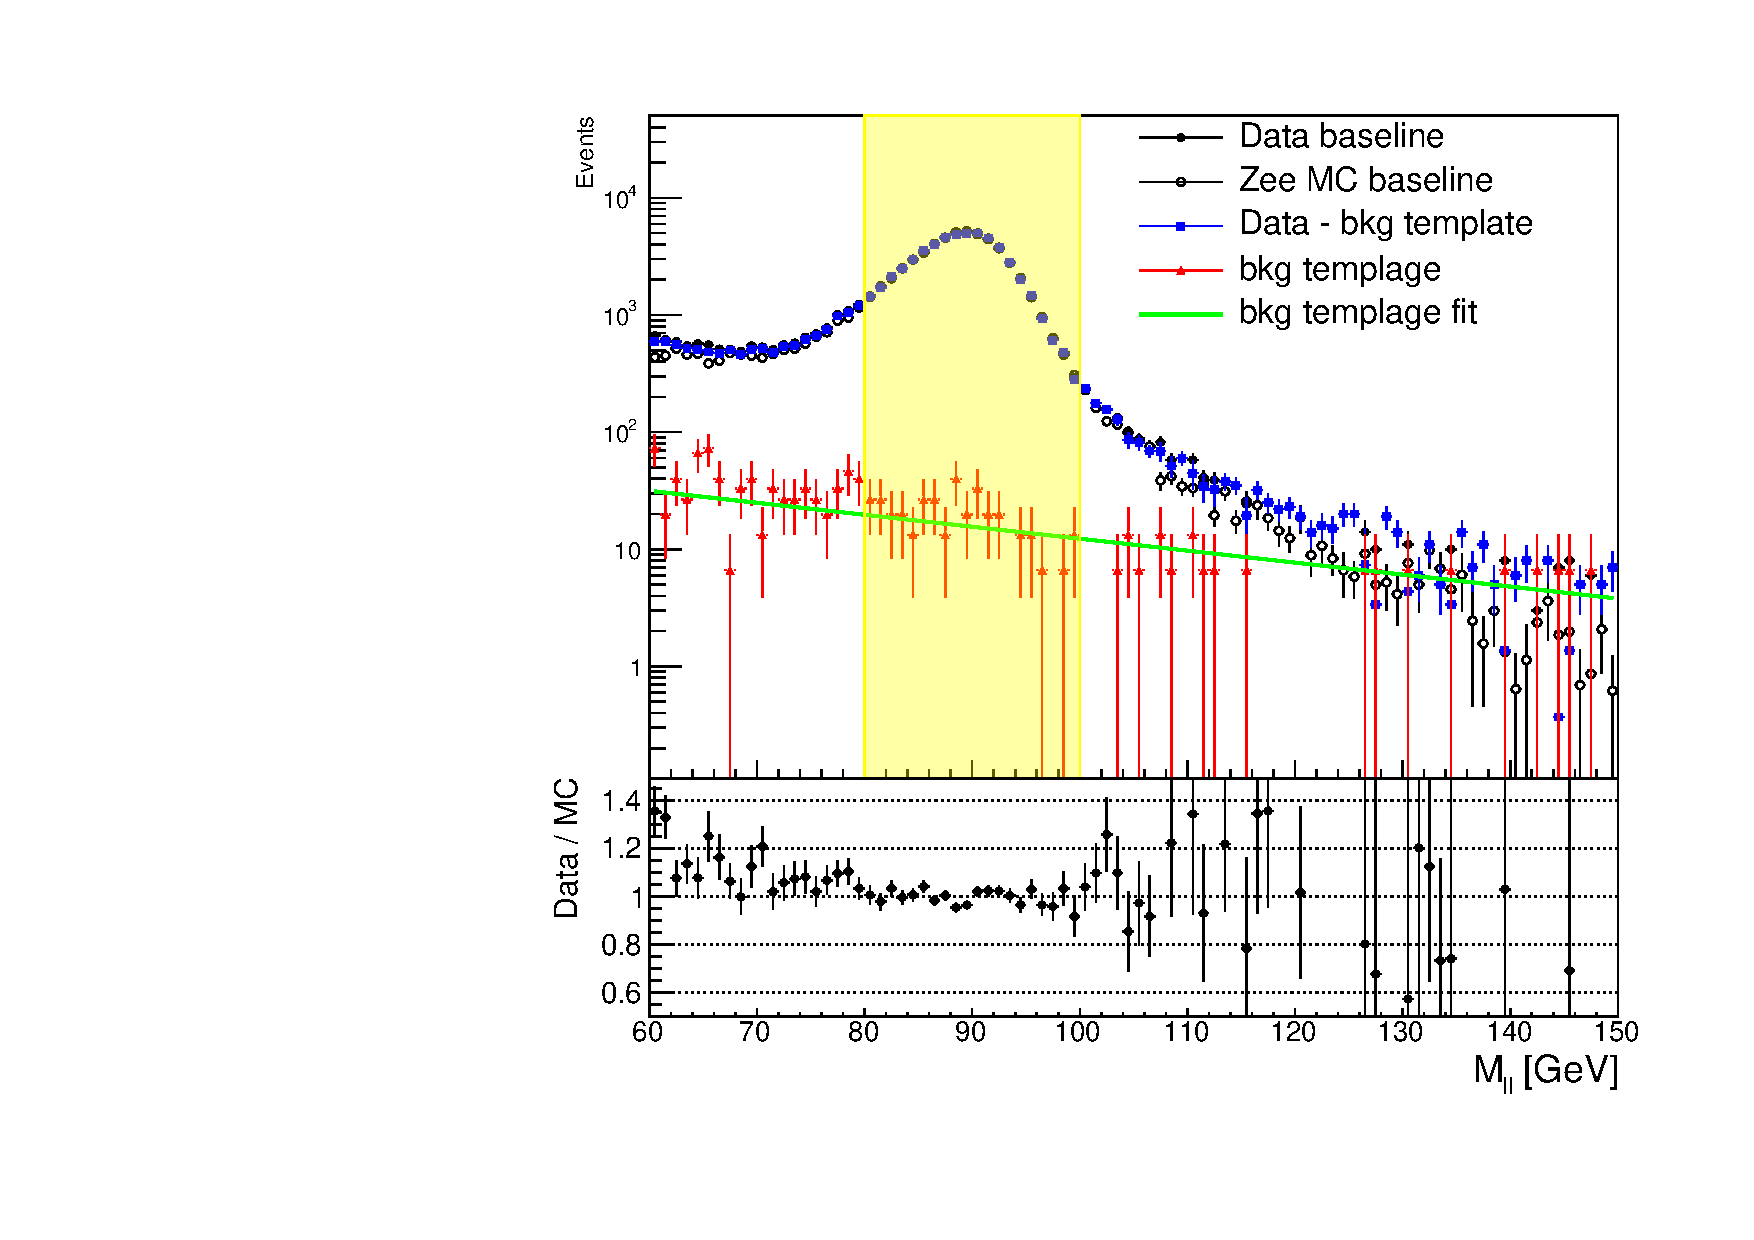
\includegraphics[scale=0.27]{bkg_subtraction_baseline_template_range_baseline_mll80_100_pt15_20_eta80_137_tag_trigger_matched.pdf}
            \caption{$15 < \pt < 20$~{\GeV}\\$0.8 < |\eta| < 1.37$}
        \end{center}
    \end{subfigure}
    \begin{subfigure}[b]{0.32\textwidth}
        \begin{center}
            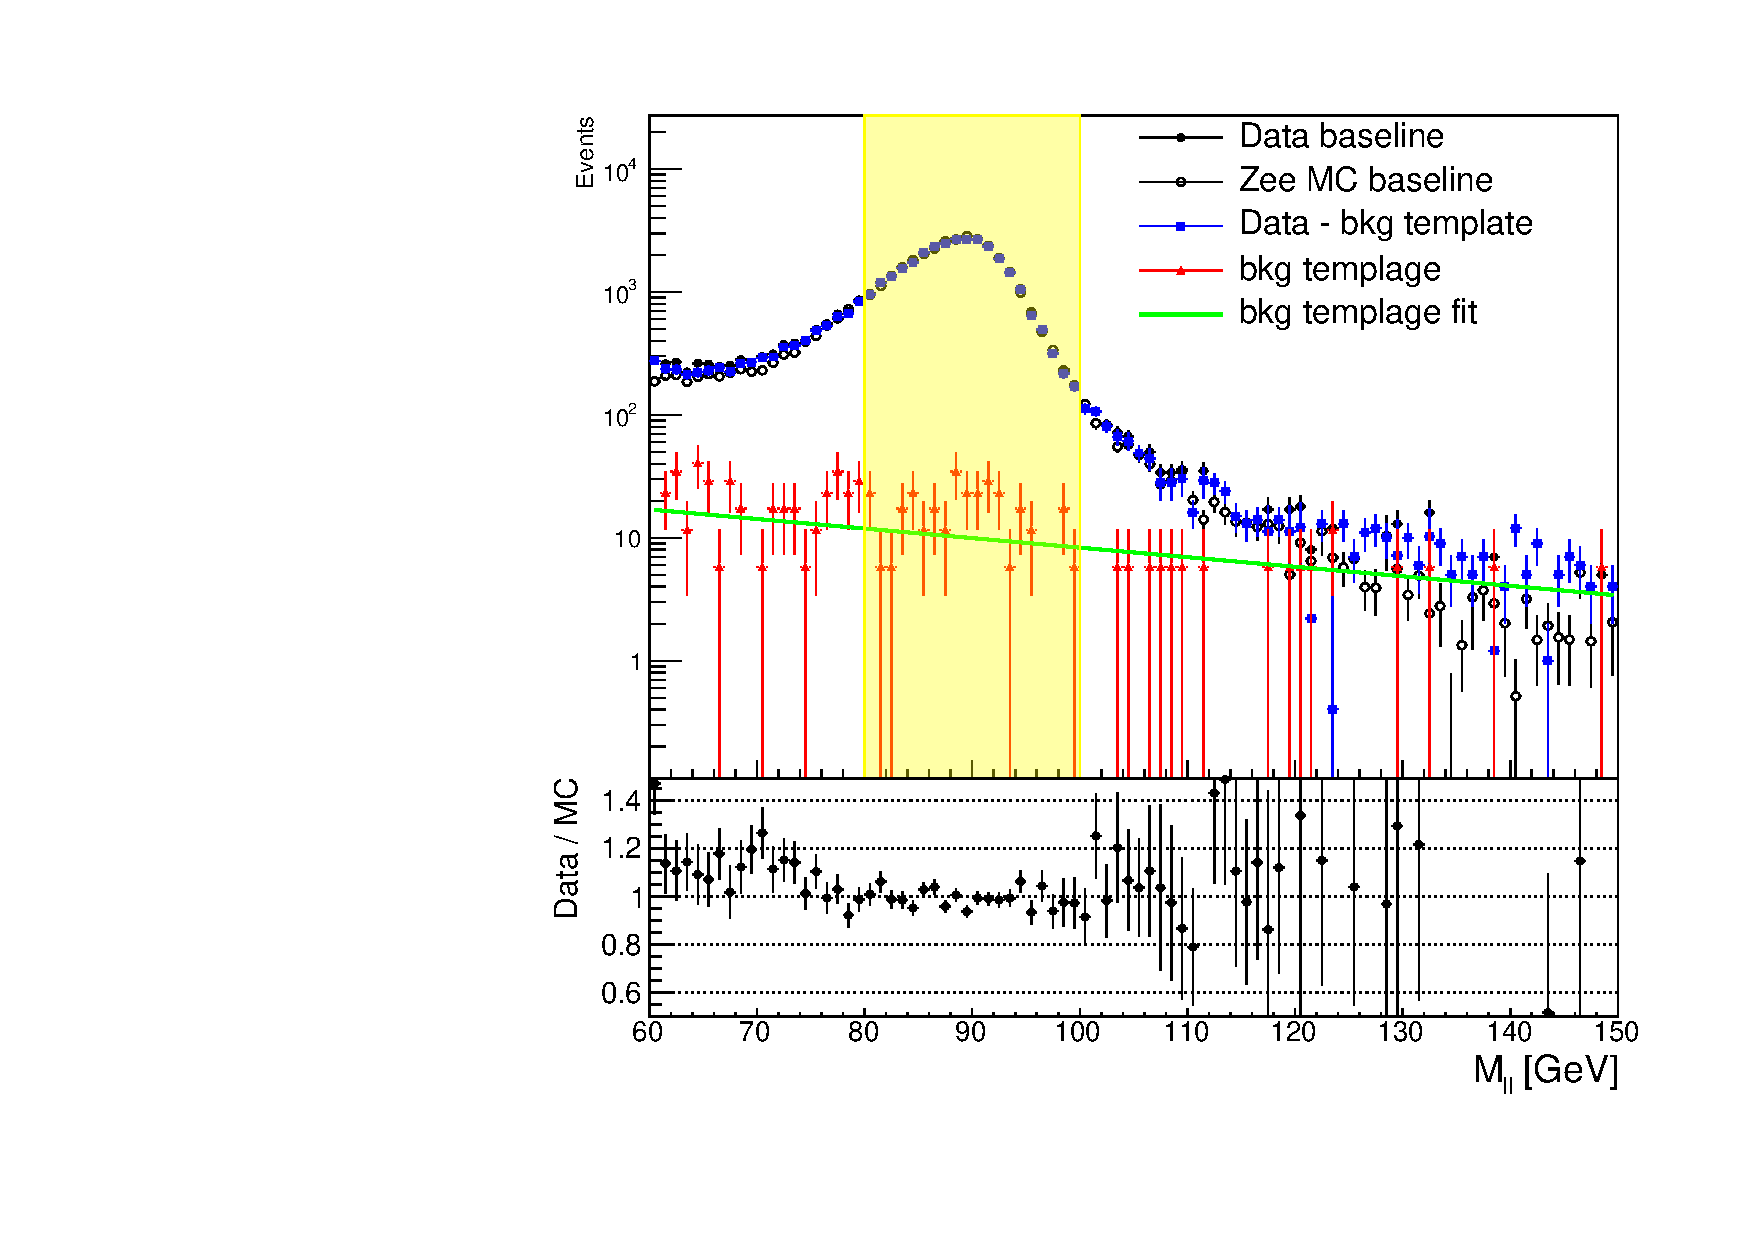
\includegraphics[scale=0.27]{bkg_subtraction_baseline_template_range_baseline_mll80_100_pt15_20_eta151_200_tag_trigger_matched.pdf}
            \caption{$15 < \pt < 20$~{\GeV}\\$1.52<|\eta|<2.0$}
        \end{center}
    \end{subfigure}
    \caption{Illustration of the background subtraction procedure.
    The full black dots and blue squares are the $m_{ee}$ distributions for data before and after performing the background subtraction, respectively.
    The $m_{ee}$ distribution for $Z \to ee$ MC, which is labeled by the open black circles, is normalized to the data after the background subtraction using a Gaussian fit of $85 < m_{ee} < 95$~{\GeV}.
    The lower panels show the data-to-MC ratio where the background subtraction has been applied on data.
    The background templates and their respective fitting results are indicated by the red triangles and green lines, respectively.
    }
    \label{fig:app_RLE_bkg_estimations}
\end{figure}
%
The data after performing the background subtraction, the MC simulation samples, the background template distributions, and the fitting results are also shown.
The simulated $m_{ee}$ distribution of $Z \to ee$ MC are normalized to the data, which background subtraction has been performed, using a Gaussian fit in $Z$ peak region $85 < m_{ee} < 95$~{\GeV}.
After performing the background subtraction, the data and MC have good agreement within the statistical uncertainties.

Then, the background contamination in the $Z$ mass region $80 < m_{ee} < 100$~{\GeV} is calculated using
%
\begin{equation}
    N_{bkg}^{80 < m_{ee} < 100~{\GeV}} = \int_{80}^{100} N_\mathrm{template} \ dm_{ee} \cdot \frac{N_{bkg}^\mathrm{tail}}{N_\mathrm{template}^\mathrm{tail}}
    \label{eq:RLE_bkg_in_80_mll_100}
\end{equation}
%
Table~\ref{tab:app_RLE_bkg_estimations} summarize the background estimations in different \pt and $|\eta|$ regions.
%
\begin{table}[htbp]
    \begin{center}
        \begin{tabular}{cccc}
            \hline
            \hline
                                  & $0 < |\eta| < 0.8$ & $0.8 < |\eta| < 1.37$ & $1.52 < |\eta| < 2.0$\\
            \hline
            $10< \pt < 15$~{\GeV} & 4.04\%             & 2.10\%                & 3.17\%\\
            $15< \pt < 20$~{\GeV} & 0.44\%             & 0.58\%                & 0.76\%\\
            \hline
            \hline
        \end{tabular}
    \end{center}
    \caption{The estimated background contamination in in different \pt and $|\eta|$ regions.
    The \pt and $|\eta|$ binnings correspond to the one used for the final measurements.}
    \label{tab:app_RLE_bkg_estimations}
\end{table}
%
The largest improvements are observed in the lowest \pt bin ($10 < \pt < 15$~{\GeV}) where a sizeable background contamination is subtracted.
The background contamination is relatively small in the second lowest \pt bin ($15 < \pt < 20$~{\GeV}) providing the evidence that high purity of prompt leptons can be obtained using $Z$ tag-and-probe method.
Table~\ref{tab:app_RLE_efficiency_before_and_after_background_subtraction} shows the real electron efficiencies before and after performing the background subtraction.

\begin{table}[htbp]
    %\begin{center}
    \resizebox{\textwidth}{!}{% <------ Don't forget this %
        \begin{tabular}{ccccc}
            \hline
            \hline
                                                    & background subtraction & $0 < |\eta| < 0.8$ & $0.8 < |\eta| < 1.37$ & $1.52 <| \eta| < 2.0$\\
            \hline
            \multirow{2}{*}{$10 < \pt < 15$~{\GeV}} & before                 & $57.4 \pm 0.9$     & $66.6 \pm 0.8$        & $53.2 \pm 0.9$\\
                                                    & after                  & $59.9 \pm 1.9$     & $68.0 \pm 1.8$        & $55.0 \pm 1.7$\\
            \hline
            \multirow{2}{*}{$15 < \pt < 20$~{\GeV}} & before                 & $64.5 \pm 0.2$     & $69.4 \pm 0.2$        & $62.0 \pm 0.3$\\
                                                    & after                  & $64.8 \pm 0.5$     & $69.8 \pm 0.5$        & $62.5 \pm 0.6$\\
            \hline
            \hline
        \end{tabular}
    }
    %\end{center}
    \caption{The real electron efficiencies before and after performing the background subtraction in different \pt and $|\eta|$ regions are shown in percentage.}
    \label{tab:app_RLE_efficiency_before_and_after_background_subtraction}
\end{table}

%%%
%%%
%%%

\section{Cut efficiencies}
\label{sec:app_RLE_cut_efficiencies}
Figure~\ref{fig:app_RLE_cut_efficiencies} shows the efficiencies associated to each signal cut with respect to baseline definitions.
%
\begin{figure}[htbp]
    \begin{subfigure}[b]{0.48\textwidth}
        \begin{center}
            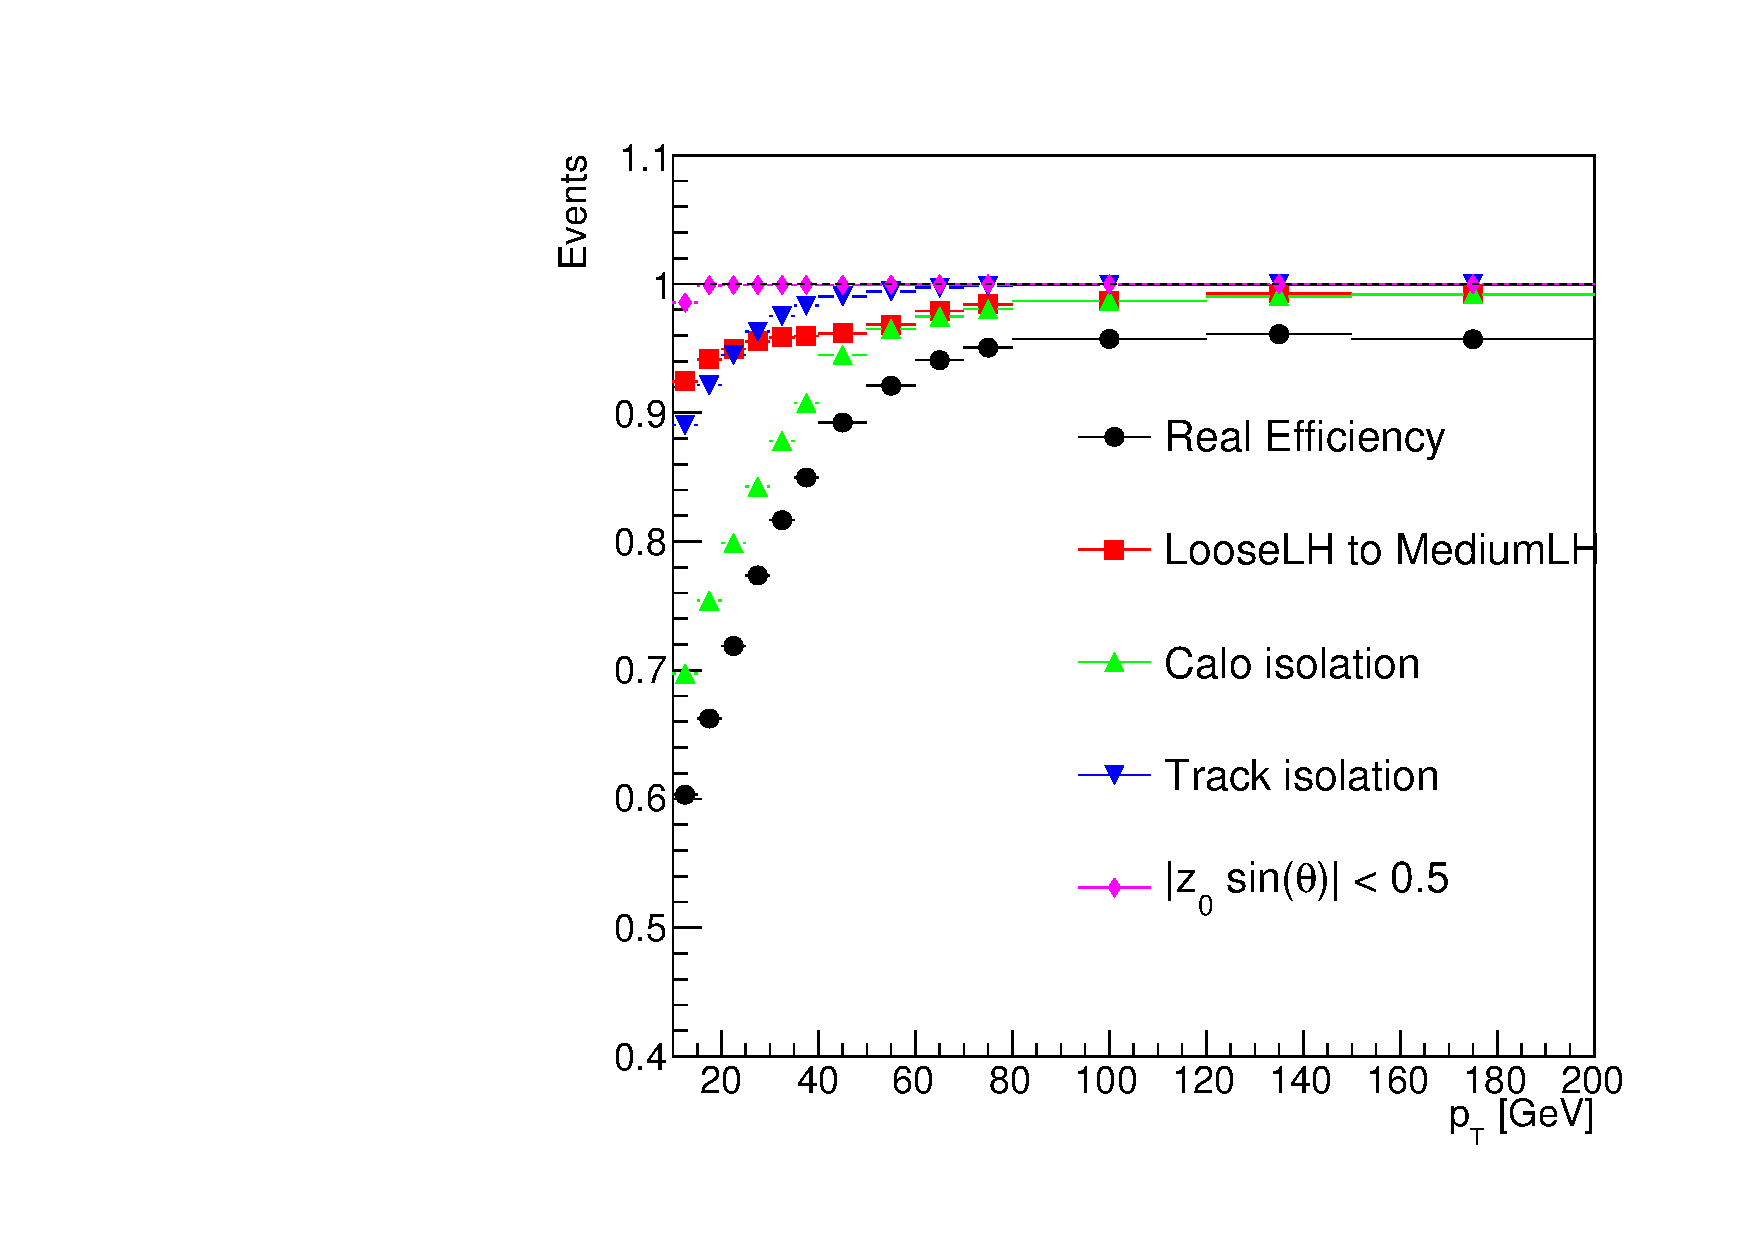
\includegraphics[scale=0.4]{cut_efficiency_electron.pdf}
            \caption{Electron}
        \end{center}
    \end{subfigure}
    \begin{subfigure}[b]{0.48\textwidth}
        \begin{center}
            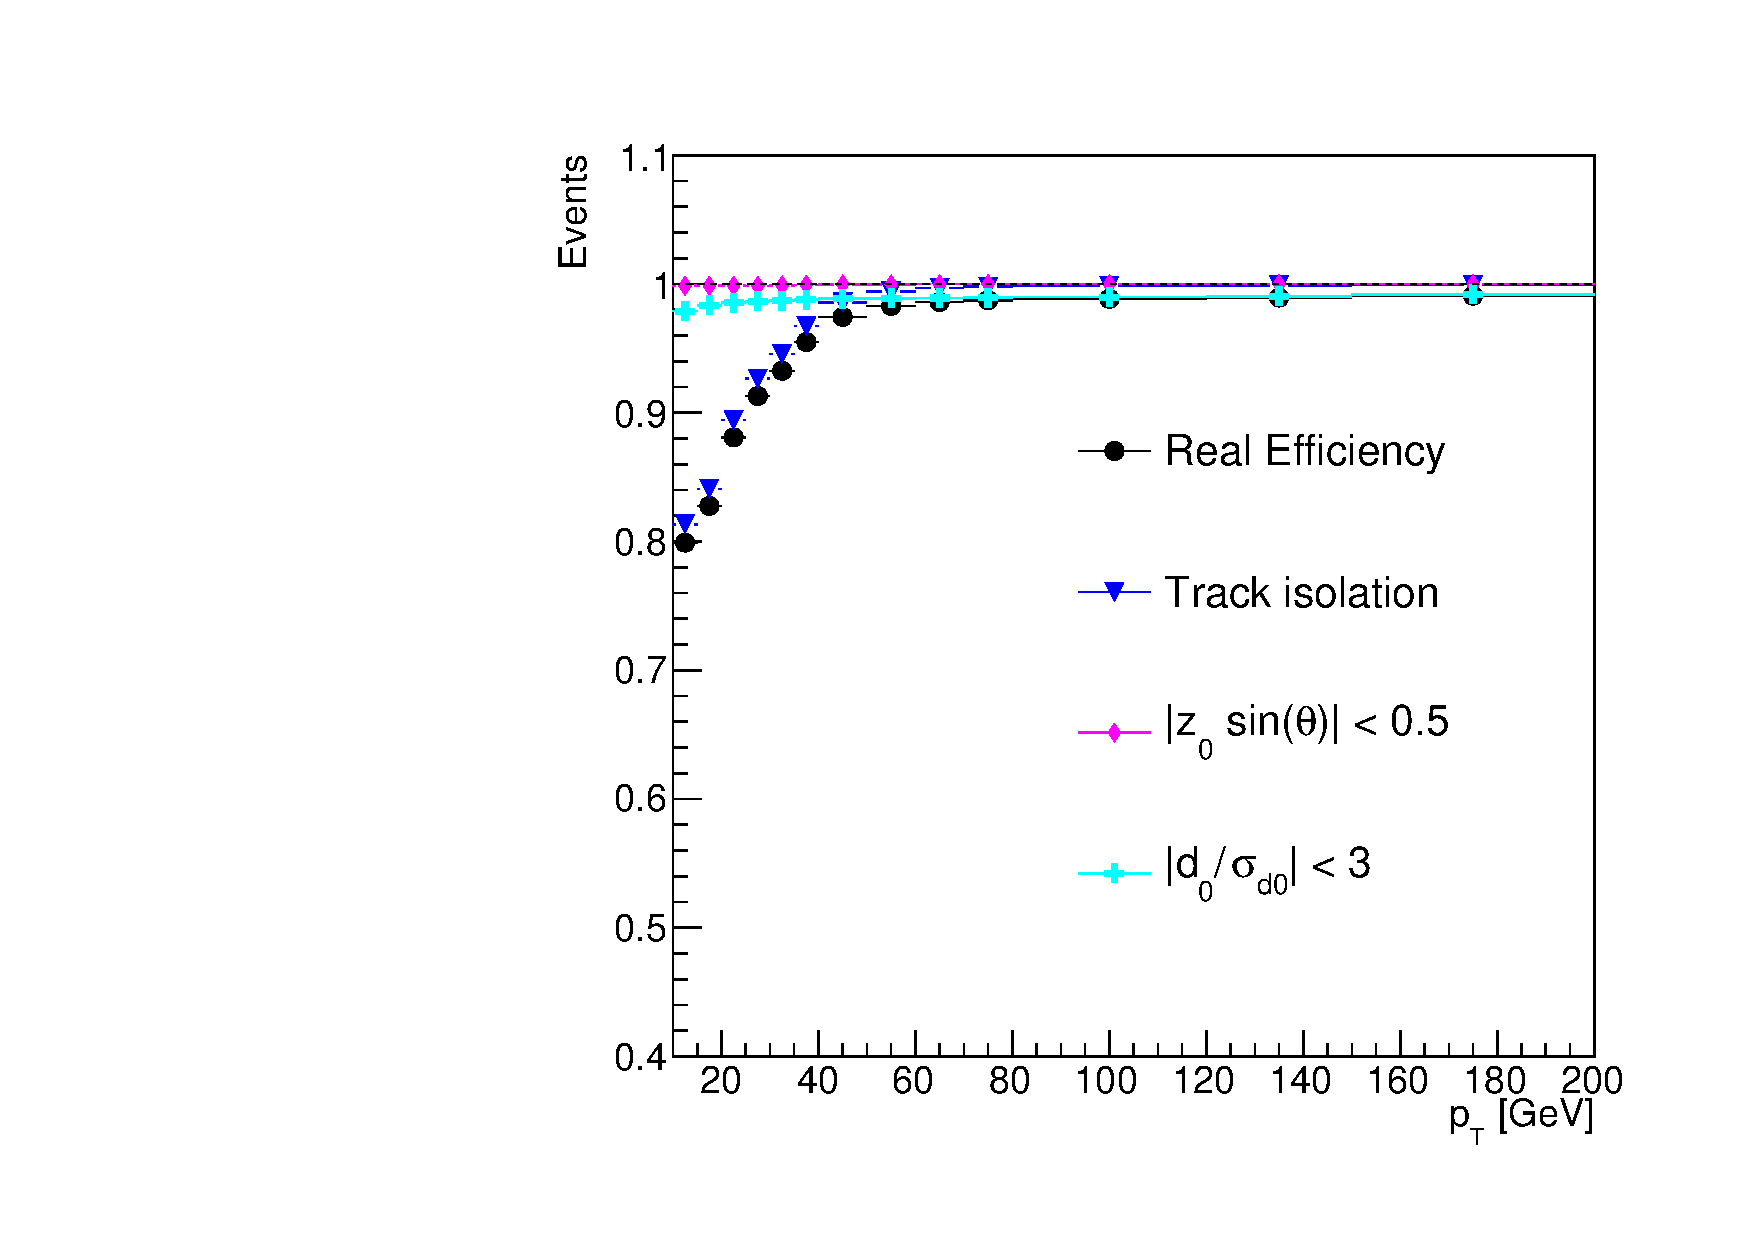
\includegraphics[scale=0.4]{cut_efficiency_muon.pdf}
            \caption{Muon}
        \end{center}
    \end{subfigure}
    \caption{Cut efficiencies of the signal electron and muon definition as a function of \pt.
    The total real electron and muon efficiencies are presented by black points. 
    The loose to medium likelihood cut efficiency is presented by red squares.
    The calorimeter and track isolation cut efficiencies are presented by green triangles and blue triangles, respectvely.
    The longitudinal and tranverse impact parameters cut efficiencies are presented by magenta diamonds and cyan crosses, respectively.}
    \label{fig:app_RLE_cut_efficiencies}
\end{figure}
%
The prompt electron efficiency increases with \pt from $\sim$62\% to $\sim$98\% and the efficiency losses are dominated by the calorimeter isolation.
The calorimeter isolation cut efficiency increases with \pt from $\sim$ 69\% to $\sim$98\%.
The loose to medium likelilihood (LH) cut efficiency increases from $\sim$92\% to $\sim$96\% in the $10< \pt < 30$~{\GeV} then reaches a plateau when $30 < \pt < 50$~{\GeV} and increases again to $\sim$98\% when $\pt > 60$~{\GeV}.
The track isolation cut efficiency increases from $\sim$89\% at low \pt to $\sim$100\% when $\pt > 60$~{\GeV}.
The longitudinal impact parameter cut efficiency increases from $\sim$98\% at low \pt to $\sim$100\% when $\pt > 15$~{\GeV}.
The cut efficiencies for muon are much higher than the electron case because the same muon identification is used for the baseline and the signal muon definitions.
The associated efficiencies computed using $Z\to \mu \mu$ events increase from $\sim$80\% for $10 < \pt < 15$~{\GeV} to $\sim$98\% when $\pt > 50$~{\GeV}.
The dominant contribution is the track isolation cut efficiency which increases from $\sim$82\% to 98\% when $\pt > 50$~{\GeV}.
The transverse and longitudinal impact parameter cut efficiencies are $\sim$99\% and 100\%, respectively.
For the electron case, the transverse impact parameter cut is already applied at the baseline level

%%%
%%%
%%%

\section{Real lepton efficiencies}
\label{sec:app_RLE}
The real lepton efficiencies as a function of \pt and $|\eta|$ are shown in Fig~\ref{fig:app_RLE_real_efficiency_total_systematics} where the background subtraction has been applied on the electron case in $10 < \pt < 15$~{\GeV} and $15 < \pt < 20$~{\GeV}.
%
\begin{figure}[htbp]
    \begin{subfigure}[b]{0.48\textwidth}
        \begin{center}
            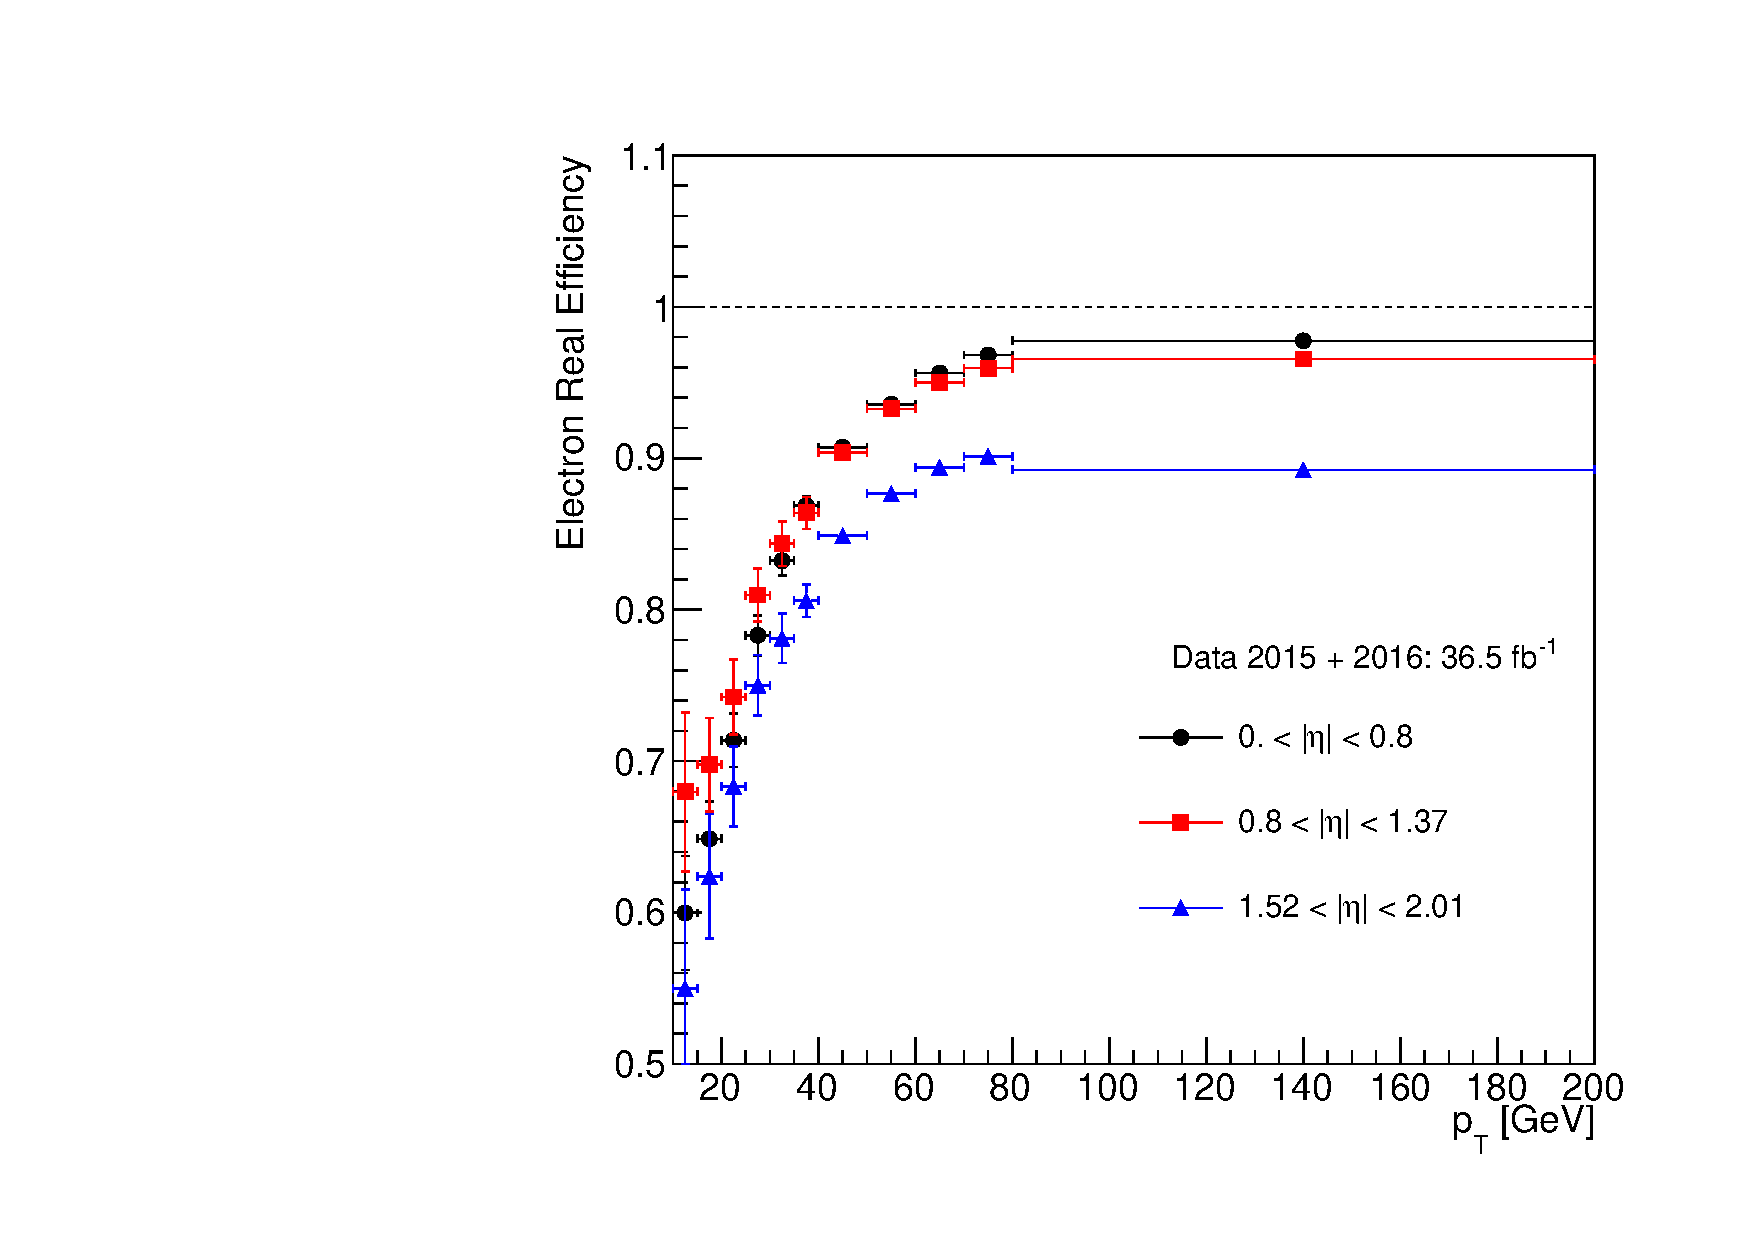
\includegraphics[scale=0.4]{real_electron_efficiency_total_systematics.pdf}
            \caption{Electron}
        \end{center}
    \end{subfigure}
    \begin{subfigure}[b]{0.48\textwidth}
        \begin{center}
            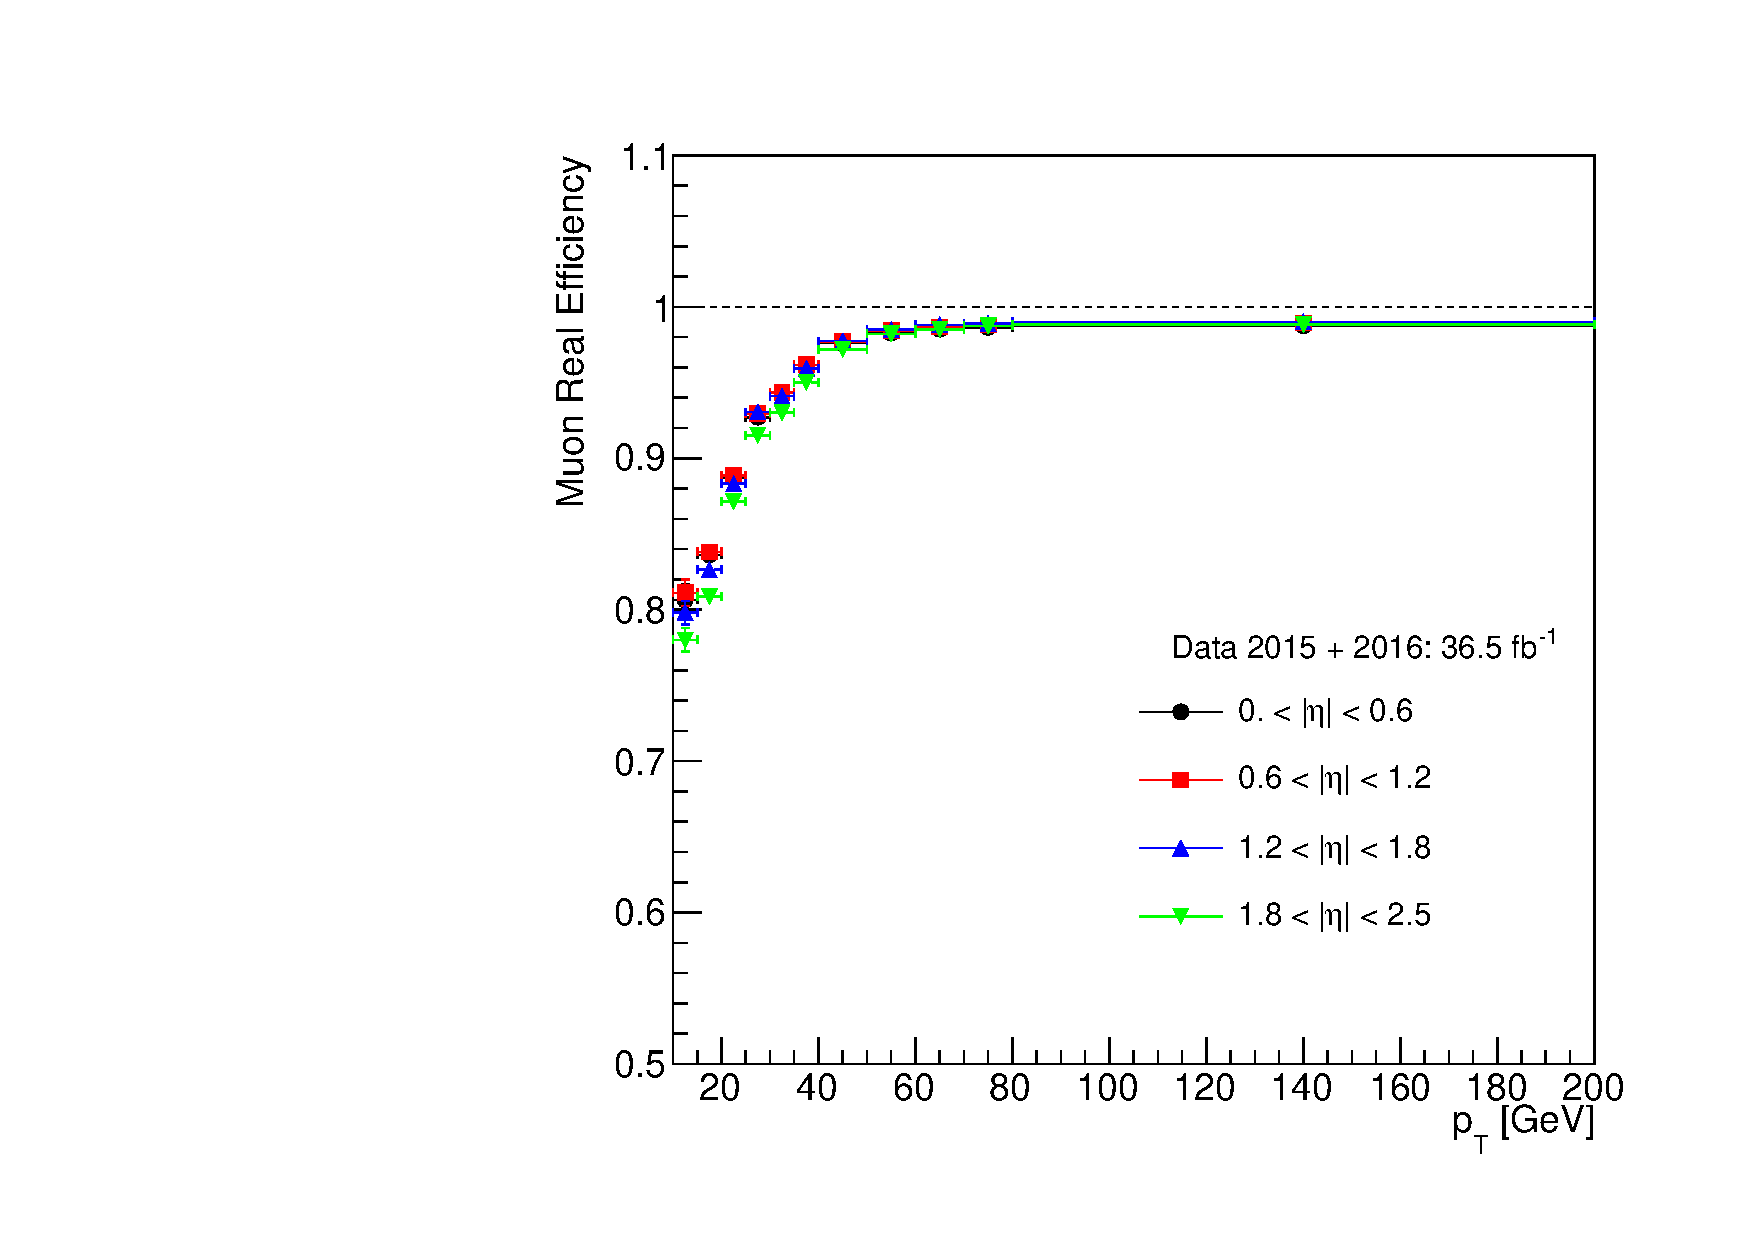
\includegraphics[scale=0.4]{real_muon_efficiency_total_systematics.pdf}
            \caption{Muon}
        \end{center}
    \end{subfigure}
    \caption{The real lepton efficiencies as a function of \pt and $|\eta|$ measured using the $Z$ tag-and-probe method.
    For the real electron efficiencies measurement, the $|\eta|$ binning in the creak region is removed.
    A homogeneous $|\eta|$ binnings are used for the muon case.}
    \label{fig:app_RLE_real_efficiency_total_systematics}
\end{figure}
%
The uncertainties are the quadratic sum of the statistical uncertainties and the measurement systematic uncertainties.
The 3 $|\eta|$ binnings for the electron case are driven by the geometry of ECAL.
The crack region, $1.37<|\eta|<1.52$, is removed from the real electron efficiency study.
It is expected that the electron efficiencies in $1.52<|\eta|<2.01$ are lower because the electron identification is better in the central region of the ECAL.

%%%
%%%
%%%

\subsection{Tag-and-probe method and truth matching comparisons}
\label{subsec:app_RLE_truth_matched}
The truth matched information in the $Z \to \ell \ell$ MC samples are used to verify the accuracy of $Z$ tag-and-probe method.
Figure~\ref{fig:app_RLE_TandP_truth_match_comparisons} shows the real lepton efficiencies as a function of \pt, $|\eta|$, and $\Delta R(\ell, \mathrm{jet})$ using $Z$ tag-and-probe method and truth matching.
%
\begin{figure}[htbp]
    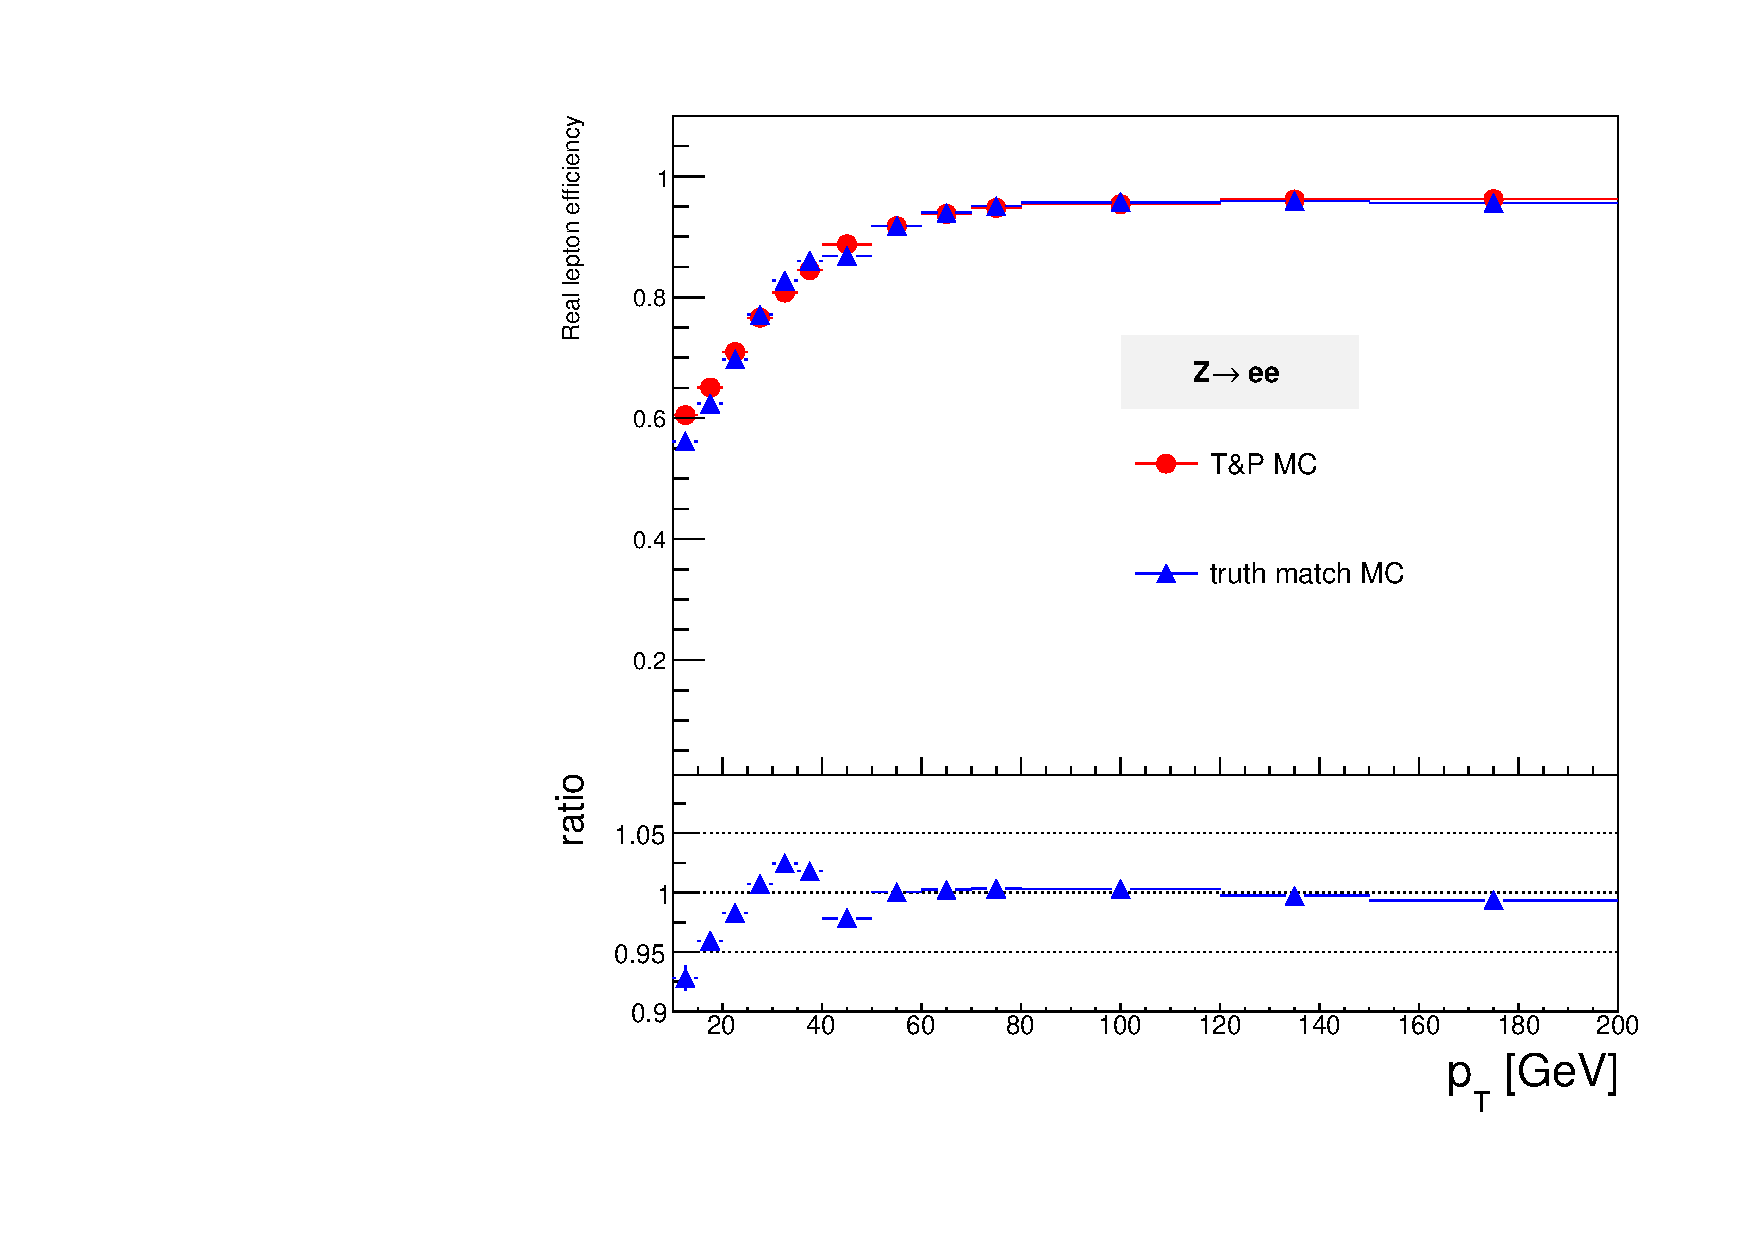
\includegraphics[width=0.32\textwidth]{Compare_TandP_truth_match_electron_pt.pdf}
    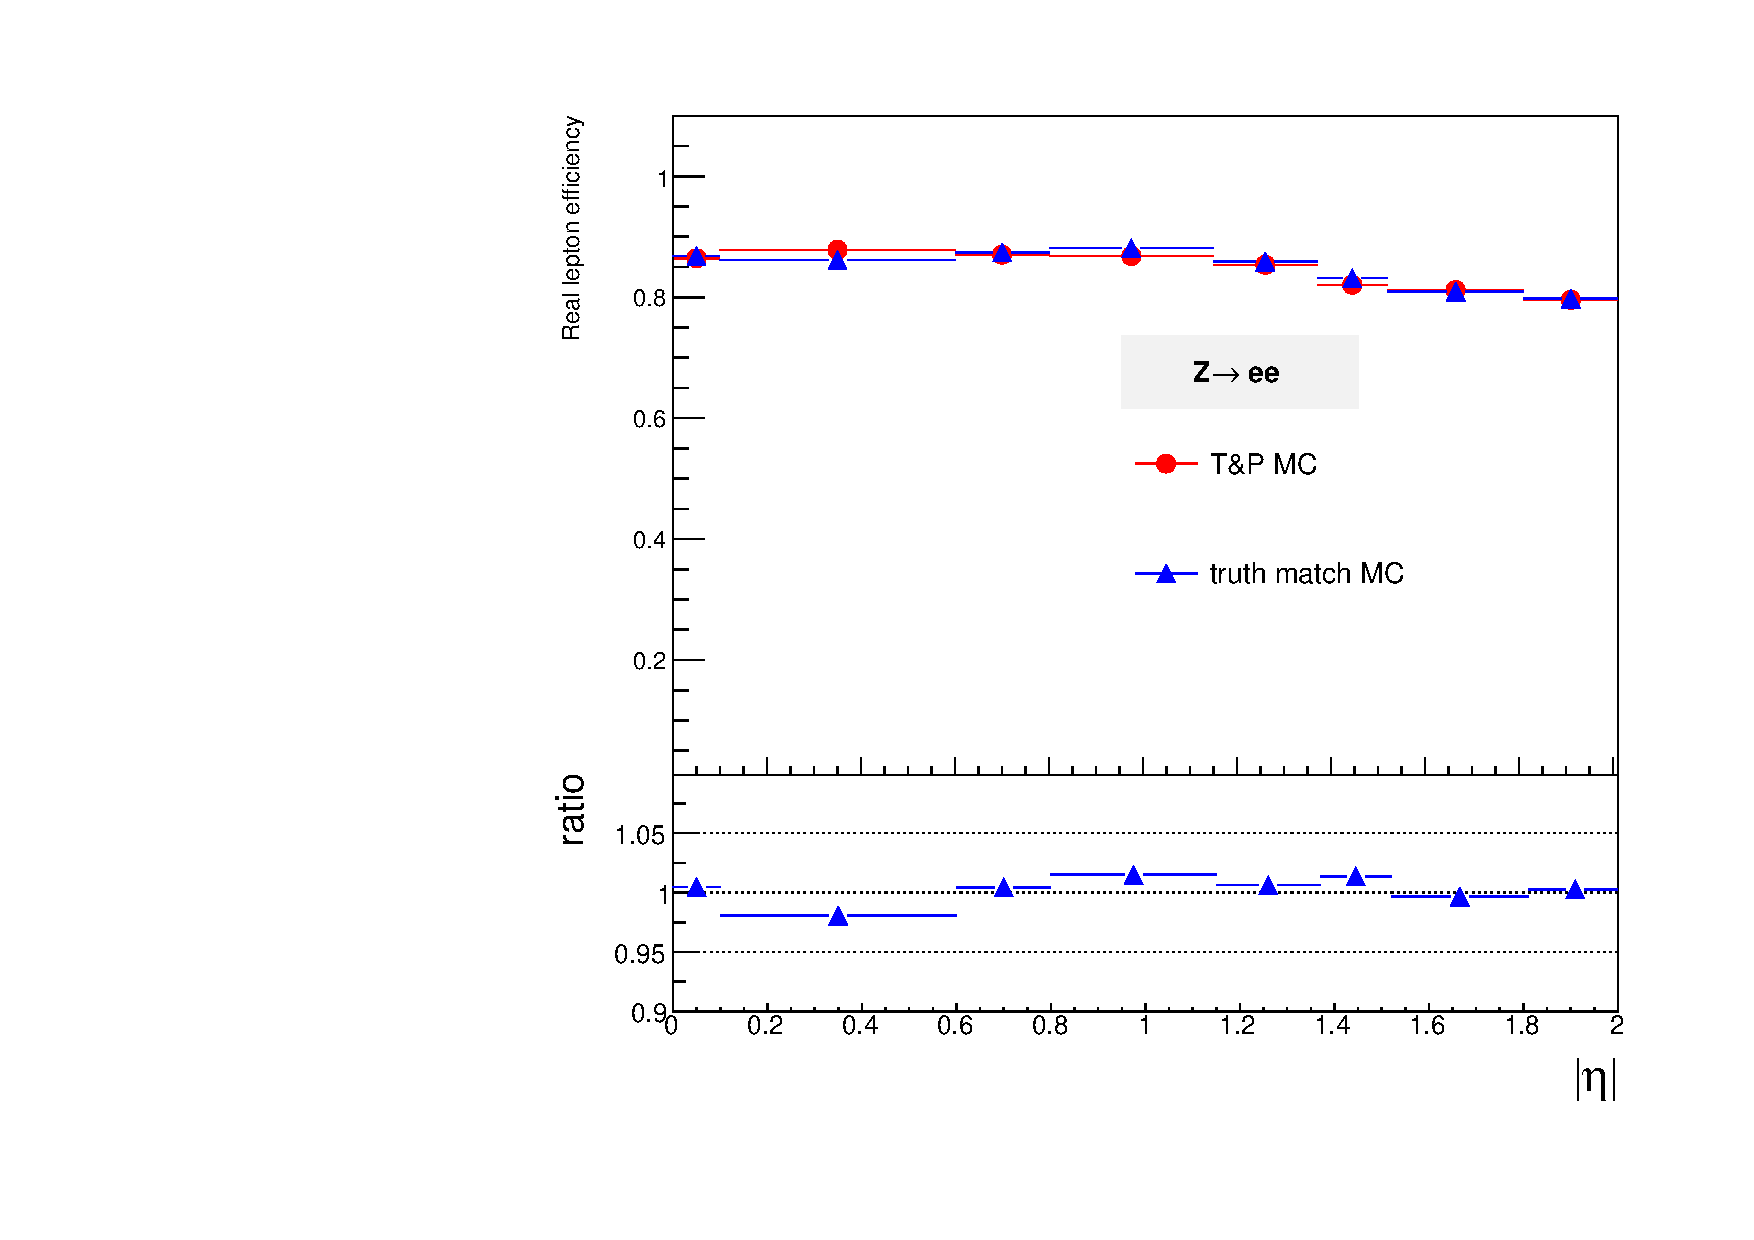
\includegraphics[width=0.32\textwidth]{Compare_TandP_truth_match_electron_eta.pdf}
    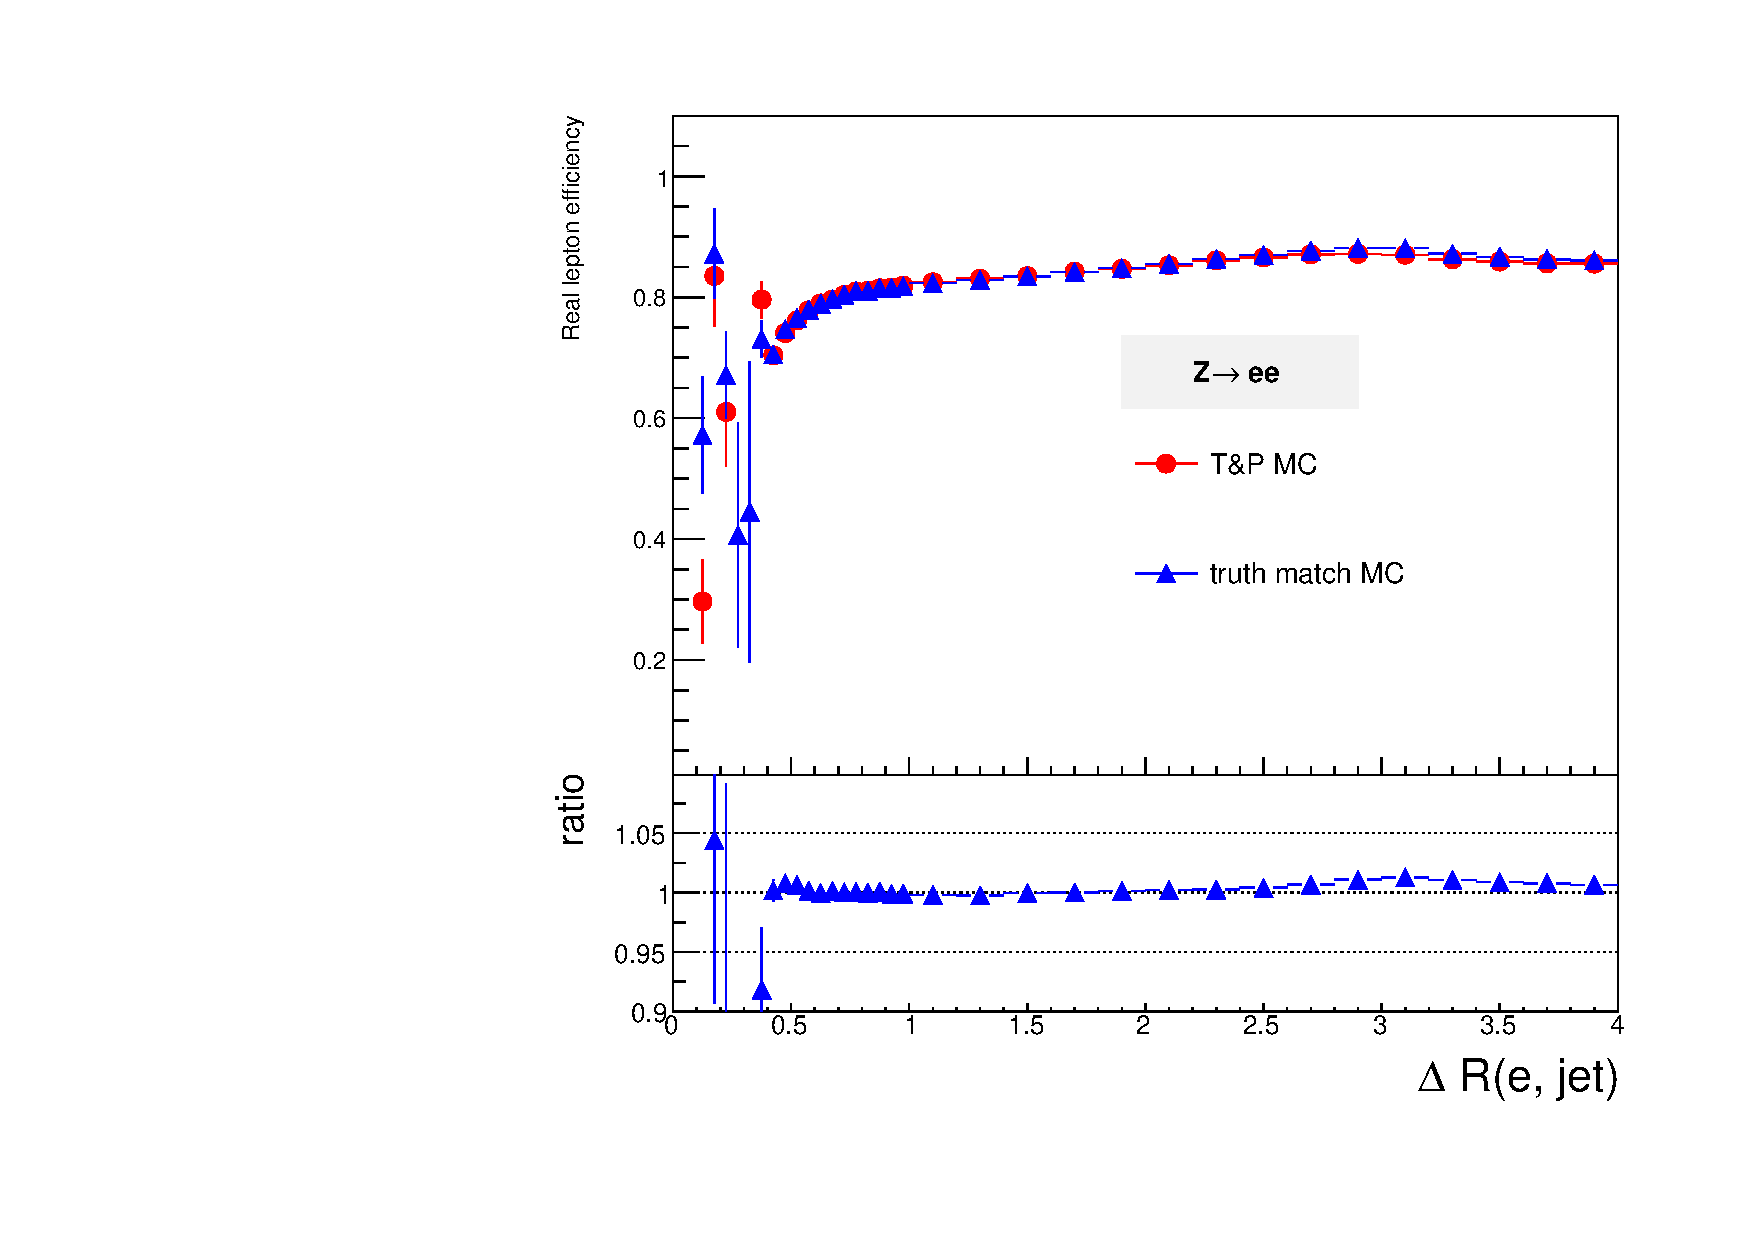
\includegraphics[width=0.32\textwidth]{Compare_TandP_truth_match_electron_dRjet.pdf}\\
    \includegraphics[width=0.32\textwidth]{Compare_TandP_truth_match_muon_pt.pdf}
    \includegraphics[width=0.32\textwidth]{Compare_TandP_truth_match_muon_eta.pdf}
    \includegraphics[width=0.32\textwidth]{Compare_TandP_truth_match_muon_dRjet.pdf}
    \caption{The real lepton efficiencies computed by $Z$ tag-and-probe method (red dots) and truth matching (blue triangles).
    The electron cases are on the top row and muon cases are at the bottom row.
    The three columns from the left to the right are the real lepton efficiencies as a function \pt, $|\eta|$, and $\Delta R(\ell, \mathrm{jet})$, respectively.
    The lower pads show the ratio with respect to the $Z$ tag-and-probe method.}
    \label{fig:app_RLE_TandP_truth_match_comparisons}
\end{figure}
%
The associated uncertainties are statistical uncertainties only.
For the real electron efficiencies, the largest difference is $\sim$7\% in low \pt and no differences can be seen when $\pt > 50$~{\GeV}; the largest difference is $\sim$3\% in ; the larger differences in $\Delta R(e, \mathrm{jet})$ exist when $\Delta R(e, \mathrm{jet}) < 0.4$.
Because the overlap removal has been applied on the baseline electrons, the $\Delta R(e, \mathrm{jet}) < 0.4$ region lacks statistics.
For the real muon efficiencies, the differences are less then 1\% for \pt and $|\eta|$.
However, the differences are larger for $\Delta R(\mu, \mathrm{jet}) < 0.4$ also because of the overlap removal.
The small differences between two methods indicate the robust of $Z$ tag-and-probe method and the differences may be considered as the systematic uncertainties.

%%%
%%%
%%%

\subsection{Data-to-MC comparisons}
\label{subsec:app_RLE_data_to_mc_comparisons}
The real lepton efficiencies calculating by data and $Z\to \ell\ell$ MC samples are compared.
All 2015 and 2016 data are considered corresponding to an integrated luminosity of 36.5 \ifb.
All the lepton scale factors are applied on the MC samples and the simulation is reweighted to the pile-up observed in data.
Figure~\ref{fig:app_RLE_real_efficiency_pt_eta_dRjet} shows the real efficiencies as a function of \pt, $|\eta|$ and $\Delta R(\ell, \mathrm{jet})$ using data and $Z\to \ell \ell$ MC samples, respectively.
%
\begin{figure}[htbp]
    \includegraphics[width=0.32\textwidth]{real_efficiency_ratio_plot_electron_pt.pdf}
    \includegraphics[width=0.32\textwidth]{real_efficiency_ratio_plot_electron_eta.pdf}
    \includegraphics[width=0.32\textwidth]{real_efficiency_ratio_plot_electron_dRjet.pdf}\\
    \includegraphics[width=0.32\textwidth]{real_efficiency_ratio_plot_muon_pt.pdf}
    \includegraphics[width=0.32\textwidth]{real_efficiency_ratio_plot_muon_eta.pdf}
    \includegraphics[width=0.32\textwidth]{real_efficiency_ratio_plot_muon_dRjet.pdf}
    \caption{The real lepton efficiencies measured on 2015 + 2016 data (black dots) and $Z\to \ell\ell$ MC samples (red squares) using the $Z$ tag-and-probe method.
    The electron cases are on the top row and muon cases are at the bottom row.
    The three columns from the left to the right are the real lepton efficiencies as a function \pt, $|\eta|$, and $\Delta R(\ell, \mathrm{jet})$, respectively.
    The MC samples have been reweighted to the pile-up observed in data.}
    \label{fig:app_RLE_real_efficiency_pt_eta_dRjet}
\end{figure}
%
The associated uncertainties are statistical uncertainties only.
Good agreement between data and MC can be seen in the \pt and $|\eta|$ plots.
Larger differences exist in $\Delta R(\ell, \mathrm{jet})$ plots because of lacking statistics.

%%%
%%%
%%%

\subsection{Real lepton efficiency versus pileup}
\label{subsec:app_RLE_vs_pileup}
The relations between the real lepton efficiencies and the pile-up are also studied.
The efficiencies computed by 2015 + 2016 data, $Z$ tag-and-probe method and truth matching MC samples are shown in Fig.~\ref{fig:app_RLE_vs_pileup}.
%
\begin{figure}[htbp]
    \begin{subfigure}[b]{0.48\textwidth}
        \begin{center}
            \includegraphics[scale=0.4]{real_efficiency_vs_AvgMu_elec.pdf}
            \caption{Electron}
        \end{center}
    \end{subfigure}
    \begin{subfigure}[b]{0.48\textwidth}
        \begin{center}
            \includegraphics[scale=0.4]{real_efficiency_vs_AvgMu_muon.pdf}
            \caption{Muon}
        \end{center}
    \end{subfigure}
    \caption{The real lepton efficiencies as a function of the average interactions per crossing $<\mu>$.
    The data is presented in black dots,  $Z\to \ell\ell$ tag-and-probe is presented in red squares, the truth matching is presented in blue triangles, the \ttbar is presented in magenta diamonds, and $\tilde{g} \to \ttbar \widetilde{\chi^{0}_{1}}$ is presented in yellow crosses.
    The $|\eta|<2$ requirement has been applied on the \ttbar and $\tilde{g} \to \ttbar \widetilde{\chi^{0}_{1}}$ MC samples for the electron case.}
\label{fig:app_RLE_vs_pileup}
\end{figure}
%
In order to study the efficiencies with different event topologies, the \ttbar and $\tilde{g} \to \ttbar \widetilde{\chi^{0}_{1}}$ MC samples are considered.
The real electron efficiencies are $\sim$92\% at low $<\mu>$ and decrease when $<\mu>$ increases.
The measured real lepton efficiencies using $\tilde{g} \to \ttbar \widetilde{\chi^{0}_{1}}$ MC sample is lower then the data case.
The \ttbar and data have similar real electron efficiencies.
However, the real muon efficiencies for \ttbar is lower than the data because the efficiencies in $\pt < 40$~{\GeV} is lower.
If a $\pt > 40$~{\GeV} requirement is applied on the \ttbar MC sample, then the efficiencies are agreed with data.
Figure~\ref{fig:app_RLE_real_efficiency_ttbar_gtt} shows the measured real electron and muon efficiencies as a function of $\pt$ using data, $Z$ tag-and-probe method, truth matching, \ttbar, and $\tilde{g} \to \ttbar \widetilde{\chi^{0}_{1}}$ MC samples.
%
\begin{figure}[htbp]
    \begin{subfigure}[b]{0.48\textwidth}
        \begin{center}
            \includegraphics[scale=0.4]{real_efficiency_ratio_plot_electron_pt_ttbar_gtt.pdf}
            \caption{Electron}
        \end{center}
    \end{subfigure}
    \begin{subfigure}[b]{0.48\textwidth}
        \begin{center}
            \includegraphics[scale=0.4]{real_efficiency_ratio_plot_muon_pt_ttbar_gtt.pdf}
            \caption{Muon}
        \end{center}
    \end{subfigure}
    \caption{The real electron and muon efficiencies as a function of $\pt$.
    The data is presented in black dots,  $Z\to \ell\ell$ tag-and-probe is presented in red squares, the truth matching is presented in blue triangles, the \ttbar is presented in magenta diamonds, and $\tilde{g} \to \ttbar \widetilde{\chi^{0}_{1}}$ is presented in yellow crosses.
    The differences in the $\pt < 40$~{\GeV} region come from the different event topologies.}
    \label{fig:app_RLE_real_efficiency_ttbar_gtt}
\end{figure}
%
The real lepton efficiencies of \ttbar process is lower than the data one in $\pt < 40$~{\GeV} region.
The real lepton efficiencies of $\tilde{g} \to \ttbar \widetilde{\chi^{0}_{1}}$ process are lower than data in both electron and muon cases.

%%%
%%%
%%%

\section{Sources of systematic uncertainties}
\label{sec:app_RLE_sources_of_systematic_uncertainties}

%%%
%%%
%%%

\subsection{Measurement systematics}
\label{subsec:app_RLE_bkg_systematics}
The measurement systematic uncertainties of the real lepton efficiency calculated by the $Z$ tag-and-probe mothod have been studied by varying the background template definitions, the template fitting ranges, and the $m_{\ell \ell}$ windows.
The definition of 3 background templates are listed in Table~\ref{tab:app_RLE_bkg_templates}.
The additional template fitting ranges are [60 \textendash 70] $\cup$ [100 \textendash 120]~{\GeV} and [65 \textendash 75] $\cup$ [100 \textendash 120]~{\GeV}.
The two other $m_{\ell \ell}$ windows considered are $75 < m_{ee} < 105$~{\GeV} and $85 < m_{ee} < 95$~{\GeV}.
Therefore, there are 27 variations are considered in $\pt < 20$~{\GeV} and 3 variations in $\pt > 20$~{\GeV} for the electron case.
Because the background subtraction is applied on the electron case only, no background templates and template fitting ranges are considered in the muon case.
There are only 3 $m_{\ell \ell}$ window variations considered for the systematic uncertainties of real muon efficiency.
Table~\ref{tab:app_RLE_bkg_systematics_elec} and Table~\ref{tab:app_RLE_bkg_systematics_muon} show the measurement uncertainties for the electron and muon cases, respectively.

\begin{table}[htbp]
    \resizebox{\textwidth}{!}{% <------ Don't forget this %
        \begin{tabular}{cccc}
            \hline
            \hline
            \multicolumn{4}{c}{Electrons (measurement)}\\
            \hline
            $|\eta|$                 & [0, 0.8]                          & [0.8, 1.37]                       & [1.52, 2.0]\\
            \hline
            $10 < \pt < 15$~{\GeV}   & 2.32\%(t) / 2.85\%(f) / 5.06\%(m) & 4.84\%(t) / 1.99\%(f) / 5.66\%(m) & 5.90\%(t) / 0.28\%(f) / 10.31\%(m)\\
            $15 < \pt < 20$~{\GeV}   & 1.39\%(t) / 0.00\%(f) / 3.55\%(m) & 2.01\%(t) / 0.01\%(f) / 3.94\%(m) & 2.05\%(t) / 0.15\%(f) / 6.19\%(m)\\
            $20 < \pt < 25$~{\GeV}   & 2.46\%                            & 3.34\%                            & 3.88\%\\
            $25 < \pt < 30$~{\GeV}   & 1.69\%                            & 2.17\%                            & 2.66\%\\
            $30 < \pt < 35$~{\GeV}   & 1.19\%                            & 1.75\%                            & 2.07\%\\
            $35 < \pt < 40$~{\GeV}   & 0.70\%                            & 1.23\%                            & 1.32\%\\
            $40 < \pt < 50$~{\GeV}   & 0.20\%                            & 0.30\%                            & 0.42\%\\
            $50 < \pt < 60$~{\GeV}   & 0.15\%                            & 0.17\%                            & 0.20\%\\
            $60 < \pt < 70$~{\GeV}   & 0.13\%                            & 0.14\%                            & 0.21\%\\
            $70 < \pt < 80$~{\GeV}   & 0.10\%                            & 0.17\%                            & 0.18\%\\
            $80 < \pt < 120$~{\GeV}  & 0.12\%                            & 0.11\%                            & 0.19\%\\
            $120 < \pt < 150$~{\GeV} & 0.10\%                            & 0.16\%                            & 0.06\%\\
            $150 < \pt < 200$~{\GeV} & 0.11\%                            & 0.03\%                            & 0.19\%\\
            \hline
            \hline
        \end{tabular}
    }
    \caption{The systematic uncertainties for real electron efficiencies.
    For the electron case, the background subtraction is applied on the first two \pt bins ($\pt < 20$~{\GeV}).
    There are 3 sources of the systematic uncertainties: varying templates (t), varying fitting ranges (f), and varying $m_{\ell \ell}$ windows (m).
    When $\pt > 20$~{\GeV}, only $m_{\ell\ell}$ window variation is considered.}
    \label{tab:app_RLE_bkg_systematics_elec}
\end{table}

\begin{table}[htbp]
    \begin{center}
    %\resizebox{\textwidth}{!}{%
        \begin{tabular}{ccccc}
            \hline
            \hline
            \multicolumn{5}{c}{Muon (measurement)}\\
            \hline
            $|\eta|$                 & [0, 0.6] & [0.6, 1.2] & [1.2, 1.8] & [1.8, 2.5]\\
            \hline
            $10 < \pt < 15$~{\GeV}   & 1.29\%   & 1.06\%     & 0.96\%     & 0.98\%\\
            $15 < \pt < 20$~{\GeV}   & 0.44\%   & 0.38\%     & 0.56\%     & 0.64\%\\
            $20 < \pt < 25$~{\GeV}   & 0.19\%   & 0.22\%     & 0.38\%     & 0.56\%\\
            $25 < \pt < 30$~{\GeV}   & 0.09\%   & 0.12\%     & 0.22\%     & 0.36\%\\
            $30 < \pt < 35$~{\GeV}   & 0.06\%   & 0.11\%     & 0.23\%     & 0.32\%\\
            $35 < \pt < 40$~{\GeV}   & 0.05\%   & 0.07\%     & 0.13\%     & 0.26\%\\
            $40 < \pt < 50$~{\GeV}   & 0.04\%   & 0.04\%     & 0.05\%     & 0.07\%\\
            $50 < \pt < 60$~{\GeV}   & 0.06\%   & 0.06\%     & 0.09\%     & 0.07\%\\
            $60 < \pt < 70$~{\GeV}   & 0.06\%   & 0.07\%     & 0.08\%     & 0.08\%\\
            $70 < \pt < 80$~{\GeV}   & 0.06\%   & 0.08\%     & 0.11\%     & 0.05\%\\
            $80 < \pt < 120$~{\GeV}  & 0.07\%   & 0.07\%     & 0.12\%     & 0.07\%\\
            $120 < \pt < 150$~{\GeV} & 0.06\%   & 0.06\%     & 0.15\%     & 0.05\%\\
            $150 < \pt < 200$~{\GeV} & 0.09\%   & 0.11\%     & 0.15\%     & 0.06\%\\
            \hline
            \hline
        \end{tabular}
    %}
    \end{center}
    \caption{The systematic uncertainties for real muon efficiencies.
    Only the $m_{\ell\ell}$ window variation is considered because no background subtraction is applied on the muon case.}
    \label{tab:app_RLE_bkg_systematics_muon}
\end{table}

Since electrons extracted from the $m_{\ell \ell}$ tail region are affected by bremsstrahlung effects, the contribution of the $m_{\ell \ell}$ window variations is larger in the systematic uncertainties.
Using larger $m_{\ell \ell}$ window, the lower real electron efficiency we get.
In $10 < \pt < 15$~{\GeV}, the contribution comes from the $m_{\ell\ell}$ window variation is $\sim$10\% wherease the background subtraction one is $\sim$6\%.
This result shows the robustness of the background subtraction method.

%%%
%%%
%%%

\subsection{Trigger bias}
\label{subsec:app_RLE_trigger_bias}
The systematic uncertainties originate from different trigger strategies are also studied.
The leptons entering in the signal regions are required to fire one of the di-lepton triggers.
If the event fires the di-lepton trigger and the considered lepton is the leading lepton or the sub-leading lepton, then a trigger matching should be applied before the real lepton efficiency measurement.
However, if the event fires the \met trigger or the considered lepton is the third leading lepton, then no trigger matching should be applied.
The systematics uncertainties of are then assigned as the differences between the nominal values and the values measured with different trigger where the nominal value is obtained using events triggered by the single lepton triggers as listed in Table~\ref{tab:app_RLE_single_lepton_triggers}.
In order to provide unbiased probe leptons for the real lepton efficiency measurements, the tag lepton must match single lepton trigger.
Moreover, the \pt of the two leading leptons must satisfies $\pt > 20$~{\GeV}, the leptons with $\pt < 20$~{\GeV} will never be trigger matched to the di-lepton trigger.
Hence, no systematics are assigned in the region $10 < \pt < 20$~{\GeV}.
The real electron efficiencies as a function of \pt in 3 $|\eta|$ regions using different trigger strategies are shown in Fig.~\ref{fig:app_RLE_trigger_bias_electron}.
The crack region, $1.37<|\eta|<1.52$, is removed from the study.

\begin{figure}[htbp]
    \begin{subfigure}[b]{0.32\textwidth}
        \begin{center}
            \includegraphics[scale=0.4]{trigger_uncertainty_electron_eta080_ratio_plot.pdf}
            \caption{$0 < |\eta| < 0.8$}
        \end{center}
    \end{subfigure}
    \begin{subfigure}[b]{0.32\textwidth}
        \begin{center}
            \includegraphics[scale=0.4]{trigger_uncertainty_electron_eta80137_ratio_plot.pdf}
            \caption{$0.8 < |\eta| < 1.37$}
        \end{center}
    \end{subfigure}
    \begin{subfigure}[b]{0.32\textwidth}
        \begin{center}
            \includegraphics[scale=0.4]{trigger_uncertainty_electron_eta152201_ratio_plot.pdf}
            \caption{$1.52 < |\eta| < 2.01$}
        \end{center}
    \end{subfigure}
    \caption{The real electron efficiencies as a function of \pt in 3 $|\eta|$ regions.
    Four different trigger strategies are applied.
    The nominal values are obtained using the single lepton trigger with tag trigger matched.
    The differences between the nominal values and the values measured using other strategies are assigned as the systematic uncertainties.}
    \label{fig:app_RLE_trigger_bias_electron}
\end{figure}

The real muon efficiencies as a function of \pt in 4 $|\eta|$ regions using different trigger strategies are shown in Fig.~\ref{fig:app_RLE_trigger_bias_muon}.
These plots indicate that the trigger strategy does not affect the real muon efficiency measurement.

\begin{figure}[htbp]
    \begin{subfigure}[b]{0.48\textwidth}
        \begin{center}
            \includegraphics[scale=0.4]{trigger_uncertainty_muon_eta060_ratio_plot.pdf}
            \caption{$0 < |\eta| < 0.6$}
        \end{center}
    \end{subfigure}
    \begin{subfigure}[b]{0.48\textwidth}
        \begin{center}
            \includegraphics[scale=0.4]{trigger_uncertainty_muon_eta60120_ratio_plot.pdf}
            \caption{$0.6 < |\eta| < 1.2$}
        \end{center}
    \end{subfigure}
    \begin{subfigure}[b]{0.48\textwidth}
        \begin{center}
            \includegraphics[scale=0.4]{trigger_uncertainty_muon_eta120180_ratio_plot.pdf}
            \caption{$1.2 < |\eta| < 1.8$}
        \end{center}
    \end{subfigure}
    \begin{subfigure}[b]{0.48\textwidth}
        \begin{center}
            \includegraphics[scale=0.4]{trigger_uncertainty_muon_eta180250_ratio_plot.pdf}
            \caption{$1.8 < |\eta| < 2.5$}
        \end{center}
    \end{subfigure}
    \caption{The real muon efficiencies as a function of \pt in 4 $|\eta|$ regions.
    Four different trigger strategies are applied.
    The nominal values are obtained using the single lepton trigger with tag trigger matched.
    The differences between the nominal values and the values measured using other strategies are assigned as the systematic uncertainties.}
    \label{fig:app_RLE_trigger_bias_muon}
\end{figure}

Table~\ref{tab:app_RLE_trigger_syst_elec} and Table~\ref{tab:app_RLE_trigger_syst_muon} show the systematic uncertainties due to the different trigger stratagies.

\begin{table}[htbp]
    \begin{center}
        \begin{tabular}{cccc}
            \hline
            \hline
            \multicolumn{4}{c}{Electrons (trigger)}\\
            \hline
            $|\eta|$                 & [0, 0.8] & [0.8, 1.37] & [1.52, 2.0]\\
            \hline
            $10 < \pt < 15$~{\GeV}   & 2.46\%   & 1.32\%      & 3.02\%\\
            $15 < \pt < 20$~{\GeV}   & 0.16\%   & 0.78\%      & 1.33\%\\
            $20 < \pt < 25$~{\GeV}   & 0.29\%   & 0.84\%      & 1.18\%\\
            $25 < \pt < 30$~{\GeV}   & 1.53\%   & 2.07\%      & 2.20\%\\
            $30 < \pt < 35$~{\GeV}   & 1.28\%   & 1.63\%      & 1.81\%\\
            $35 < \pt < 40$~{\GeV}   & 0.98\%   & 1.19\%      & 1.42\%\\
            $40 < \pt < 50$~{\GeV}   & 0.73\%   & 0.90\%      & 1.05\%\\
            $50 < \pt < 60$~{\GeV}   & 0.68\%   & 0.81\%      & 1.05\%\\
            $60 < \pt < 70$~{\GeV}   & 0.61\%   & 0.70\%      & 1.13\%\\
            $70 < \pt < 80$~{\GeV}   & 0.65\%   & 0.77\%      & 1.27\%\\
            $80 < \pt < 120$~{\GeV}  & 0.60\%   & 0.66\%      & 1.11\%\\
            $120 < \pt < 120$~{\GeV} & 0.38\%   & 0.40\%      & 0.79\%\\
            $150 < \pt < 200$~{\GeV} & 0.43\%   & 0.22\%      & 0.25\%\\
            \hline
            \hline
        \end{tabular}
    \end{center}
    \caption{The systematic uncertainties for real electron efficiencies due to the different trigger strategies.
    The uncertainties of each trigger strategy are calculated with respect to the one applied single lepton trigger with tag trigger matched.
    The total uncertainties are the quadratic sum of the uncertainties of each trigger strategy.}
    \label{tab:app_RLE_trigger_syst_elec}
\end{table}

\begin{table}[htbp]
    \begin{center}
        \begin{tabular}{ccccc}
            \hline
            \hline
            \multicolumn{5}{c}{Muons (trigger)}\\
            \hline
            $|\eta|$                 & [0, 0.6] & [0.6, 1.2] & [1.2, 1.8] & [1.8, 2.5]\\
            \hline
            $10 < \pt < 15$~{\GeV}   & 0.11\%   & 0.15\%     & 0.34\%     & 0.19\%\\
            $15 < \pt < 20$~{\GeV}   & 0.14\%   & 0.50\%     & 0.75\%     & 0.77\%\\
            $20 < \pt < 25$~{\GeV}   & 0.30\%   & 0.63\%     & 1.01\%     & 0.93\%\\
            $25 < \pt < 30$~{\GeV}   & 0.90\%   & 1.38\%     & 2.12\%     & 1.83\%\\
            $30 < \pt < 35$~{\GeV}   & 0.58\%   & 0.84\%     & 1.27\%     & 0.99\%\\
            $35 < \pt < 40$~{\GeV}   & 0.33\%   & 0.37\%     & 0.57\%     & 0.46\%\\
            $40 < \pt < 50$~{\GeV}   & 0.16\%   & 0.13\%     & 0.16\%     & 0.13\%\\
            $50 < \pt < 60$~{\GeV}   & 0.06\%   & 0.06\%     & 0.07\%     & 0.07\%\\
            $60 < \pt < 70$~{\GeV}   & 0.04\%   & 0.04\%     & 0.04\%     & 0.04\%\\
            $70 < \pt < 80$~{\GeV}   & 0.05\%   & 0.06\%     & 0.04\%     & 0.06\%\\
            $80 < \pt < 120$~{\GeV}  & 0.03\%   & 0.03\%     & 0.03\%     & 0.11\%\\
            $120 < \pt < 120$~{\GeV} & 0.05\%   & 0.13\%     & 0.10\%     & 0.08\%\\
            $150 < \pt < 200$~{\GeV} & 0.04\%   & 0.03\%     & 0.02\%     & 0.19\%\\
            \hline
            \hline
        \end{tabular}
    \end{center}
    \caption{The systematic uncertainties for real muon efficiencies due to the different trigger strategies.
    The uncertainties of each trigger strategy are calculated with respect to the one applied single lepton trigger with tag trigger matched.
    The total uncertainties are the quadratic sum of the uncertainties of each trigger strategy.}
    \label{tab:app_RLE_trigger_syst_muon}
\end{table}

%%%
%%%
%%%

\subsection{Extrapolation to signal regions}
\label{subsec:app_RLE_extrapolation_to_signal_region}




































The real lepton efficiencies are measured with a sample enriched in $Z\to \ell\ell$ events characterized by well isolated leptons.
The different processes entering in the signal region are accompanied by many ($b$-)jets and with a different event topology.
Thus, the leptons presented in the final state are not necessary well isolated.
As tighter isolation cuts are used for the signal lepton definitions, their associated real efficiencies can be smaller.
A SUSY benchmark model $\tilde{g}\to\ttbar\tilde{\chi}^{0}_{1}$ is used and the boosted event topoloties are selected by applying the requirement $\Delta m=m_{\tilde{g}}-m_{\chi^{0}_{1}}>\SI{1}{TeV}$ on the model.
These differences in the real lepton efficiencies between the $Z\to \ell\ell$ processes and the $\tilde{g}\to\ttbar\tilde{\chi}^{0}_{1}$ process are assigned as system uncertainties.
As the topology of one of the main irreducible backgrounds $\ttbar V$ is close to the \ttbar one, the efficiencies measured with the leptons from \ttbar are also considered.
The efficiency comparisons are made for each $\pt$ bin considering different $\Delta R(\ell, jets)$ ranges.

The kinematic distributions of the baseline leptons from the $Z\to \ell\ell$, \ttbar, and $\tilde{g}\to\ttbar\tilde{\chi}^{0}_{1}$ are showned in Figure~\ref{fig:RLE_kinematic}.
The top row shows the \pt distributions for the baseline electrons on the left hand side and muons on the right hand side.
The bottom row shows the $|\eta|$ distributions.
These plots show that the leptons from SUSY process are more boosted and more central than the ones from $Z$ and \ttbar processes.
The $\Delta R(\ell, jet)$ and the $N_{jets}$ distributions of the baseline leptons extracted from $Z\to\ell\ell$, \ttbar, and $\tilde{g}\to\ttbar\tilde{\chi}^{0}_{1}$ processes are shown in Figure~\ref{fig:RLE_dRjet_Njet}.
The left hand side is the electron case and the right hand side is the muon case.
The $\Delta R(\ell, jet)$ distribution associated to the SUSY signals peak at 0.5 and most of the statistics are contained in $\Delta R(\ell, jet)<1$ region.
In comparison, the leptons from the $Z\to\ell\ell$ processes are not accompanied with a signal jet and the $\Delta R(\ell, jet)$ distribution peak about $\Delta R(\ell, jet)=3$.
The jet multiplicity of the $Z\to\ell\ell$ peak at 4 jets for the electron case, 3 jets for the muon case, but for the SUSY signal peaks at 9 jets.
These plots confirm that the leptons produced in the SUSY signal are accompained with many more jets and are therefore less isolated than the $Z\to\ell\ell$ processes.
This extreme topology enables us to assess a conservative SUSY signal extrapolation systematic uncertainty that should cover all SUSY signal processes considered by the analysis.

\begin{figure}[htbp]
    \includegraphics[width=0.96\textwidth]{baseline_kinematics.pdf}
    \caption{The kinematic distributions of the baseline lepton from the processes considered for the systematic uncertainty study.
    The top row shows the \pt distributions for the baseline electrons on the left hand side and muons on the right hand side.
    The bottom row shows the $|\eta|$ distributions.
    The $\tilde{g}\to\ttbar\tilde{\chi}^{0}_{1}$ process is more boosted and centralized than the $Z\to\ell\ell$ and \ttbar processes.}
    \label{fig:app_RLE_kinematic}
\end{figure}

\begin{figure}[htbp]
    \includegraphics[width=0.96\textwidth]{baseline_deltaR_and_NJets.pdf}
    \caption{The $\Delta R(\ell, jet)$ and the $N_{jets}$ distributions of the baseline leptons extracted from $Z\to\ell\ell$, \ttbar, and $\tilde{g}\to\ttbar\tilde{\chi}^{0}_{1}$ processes.
    Most of the statistics of $\tilde{g}\to\ttbar\tilde{\chi}^{0}_{1}$ are located in $\Delta R(\ell, jet)<1$ region and higher $N_{jets}$ region.
    In the contrat, the statistics of $Z\to\ell\ell$ processes are populated at higher $\Delta R(\ell, jet)<1$ region and lower $N_{jets}$ region.}
    \label{fig:app_RLE_dRjet_Njet}
\end{figure}

The real lepton efficiencies as a functionof \pt using $Z\to\ell\ell$, \ttbar, and $\tilde{g}\to\ttbar\tilde{\chi^{0}_{1}}$ are shown in Figure~\ref{fig:RLE_real_efficiency_ttbar_gtt}.
The lower panel shows the ratio with respect to the data.
In the left hand side plot shows the real electron efficiencies as a function of \pt and the right hand side shows the real muon efficiencies as a function of \pt. 
The left hand side plot shows that the real electron efficiencies are \pt dependent in the $\pt<\SI{50}{GeV}$ region and become stable when $\pt>\SI{50}{GeV}$.
The efficiencies computed using $\tilde{g}\to\ttbar\tilde{\chi^{0}_{1}}$ are about 8\% lower than the efficiencies calculated using $Z\to ee$.
The observed differences in the low \pt region are mostly due to the calorimeter isolation and the track isolation cuts.
And the track isolation and $d_{0}/\sigma_{d_{0}}$ cuts are the main reasons cause the efficiency differences in the muon real efficiencies.

The average efficiencies of $Z\to\ell\ell$ are calculated and the relative efficiency differences are computed with respect to the average efficiencies.
The relative efficiency differences as a function of $\Delta R(\ell, jet)$ are considered for each measured \pt bins and are shown in Table~\ref{tab:RLE_syst_busy}.

\begin{table}
    \resizebox{\textwidth}{!}{%
        \begin{tabular}{ccccccccc}
            \hline
            \hline
            \multicolumn{9}{c}{electrons (busy environments)}\\
            \hline
            $\Delta R(e, \mathrm{jet})$ & [0, 0.1] & [0.1, 0.15] & [0.15, 0.2] & [0.2, 0.3] & [0.3, 0.35] & [0.35, 0.4] & [0.4, 0.6] & [0.6, 4]\\
            \hline
            $10 < \pt < 20$~{\GeV}      & -        & -           & -           & -          & -           & -           & 25.31\%    & 6.5\%\\
            $20 < \pt < 30$~{\GeV}      & -        & -           & -           & -          & -           & 73.37\%     & 10.21\%    & 0.37\%\\
            $30 < \pt < 40$~{\GeV}      & -        & -           & -           & 97.71\%    & 48.22\%     & 15.54\%     & 7.29\%     & 0.58\%\\
            $40 < \pt < 50$~{\GeV}      & -        & -           & -           & 52.81\%    & 22.80\%     & 16.73\%     & 7.68\%     & 1.10\%\\
            $50 < \pt < 60$~{\GeV}      & -        & -           & -           & 29.96\%    & 21.49\%     & 20.23\%     & 6.99\%     & 2.78\%\\
            $60 < \pt < 80$~{\GeV}      & -        & -           & 55.89\%     & 24.31\%    & 17.40\%     & 24.77\%     & 6.20\%     & 2.87\%\\
            $80 < \pt < 150$~{\GeV}     & -        & 57.52\%     & 30.24\%     & 16.45\%    & 12.73\%     & 20.92\%     & 4.44\%     & 2.73\%\\
            $150 < \pt < 200$~{\GeV}    & 88.54\%  & 40.16\%     & 19.34\%     & 8.45\%     & 14.66\%     & 16.57\%     & 2.57\%     & 1.90\%\\
            \hline
            \hline
            \multicolumn{9}{c}{muons (busy environments)}\\
            \hline
            $\Delta R(\mu, \mathrm{jet})$ & [0, 0.1] & [0.1, 0.15] & [0.15, 0.2] & [0.2, 0.3] & [0.3, 0.35] & [0.35, 0.4] & [0.4, 0.6] & [0.6, 4]\\
            \hline
            $10 < \pt < 20$~{\GeV}        & -        & -           & -           & -          & -           & -           & 33.59\%    & 5.18\%\\
            $20 < \pt < 30$~{\GeV}        & -        & -           & -           & -          & -           & 82.34\%     & 22.27\%    & 3.39\%\\
            $30 < \pt < 40$~{\GeV}        & -        & -           & -           & 98.54\%    & 56.36\%     & 31.89\%     & 14.22\%    & 2.24\%\\
            $40 < \pt < 50$~{\GeV}        & -        & -           & -           & 53.10\%    & 21.33\%     & 13.90\%     & 6.81\%     & 1.45\%\\
            $50 < \pt < 60$~{\GeV}        & -        & -           & -           & 24.98\%    & 13.72\%     & 9.62\%      & 3.83\%     & 0.79\%\\
            $60 < \pt < 80$~{\GeV}        & -        & -           & 44.41\%     & 13.75\%    & 6.14\%      & 4.76\%      & 2.04\%     & 0.15\%\\
            $80 < \pt < 150$~{\GeV}       & -        & 29.94\%     & 7.14\%      & 3.16\%     & 1.30\%      & 1.04\%      & 0.07\%     & 0.57\%\\
            $150 < \pt < 200$~{\GeV}      & 82.26\%  & 4.14\%      & 1.02\%      & 0.17\%     & 0.29\%      & 0.62\%      & 1.02\%     & 1.13\%\\
            \hline
            \hline
        \end{tabular}
    }
    \caption{The systematic uncertainties of the real lepton efficiency in busy environment using $\gluino \to \ttbar \widetilde{\chi_1^0}$.}
    \label{tab:app_RLE_syst_busy}
\end{table}

%%%
%%%
%%%

\subsection{Final uncertainties}
\label{subsec:app_RLE_final_uncertainties}
The final uncertainties are the quadratic sum of the statistical uncertainties and the systematic uncertainties.
The sources of systematic uncertainty include the measurement uncertainty, the trigger uncertainty, the uncertainty comes from the differences between $Z$ tag-and-probe method and truth matching, and the uncertainty in the busy environment.
Table~\ref{tab:app_RLE_syst_busy} shows the uncertainty in the busy environment.
The uncertainty in the busy environment is measured as a function of \pT and $\Delta R$ so it doesn't combine with the other uncertainties which are function of \pT and $|\eta|$.
Table~\ref{tab:app_RLE_final_uncertainties_elec} and Table~\ref{tab:app_RLE_final_uncertainties_muon} show the final uncertainties for electron and muon real efficiencies, respectively.

\begin{table}[htbp]
    \begin{center}
        \begin{tabular}{cccc}
            \hline
            \hline
            \multicolumn{4}{c}{Electrons (final uncertainties)}\\
            \hline
            $|\eta|$                 & [0, 0.8] & [0.8, 1.37] & [1.52, 2.0]\\
            \hline
            $10 < \pt < 15$~{\GeV}   & 0.047    & 0.063       & 0.089\\
            $15 < \pt < 20$~{\GeV}   & 0.027    & 0.042       & 0.062\\
            $20 < \pt < 25$~{\GeV}   & 0.018    & 0.031       & 0.041\\
            $25 < \pt < 30$~{\GeV}   & 0.029    & 0.024       & 0.027\\
            $30 < \pt < 35$~{\GeV}   & 0.023    & 0.021       & 0.023\\
            $35 < \pt < 40$~{\GeV}   & 0.014    & 0.018       & 0.018\\
            $40 < \pt < 50$~{\GeV}   & 0.007    & 0.010       & 0.010\\
            $50 < \pt < 60$~{\GeV}   & 0.008    & 0.010       & 0.010\\
            $60 < \pt < 70$~{\GeV}   & 0.007    & 0.010       & 0.010\\
            $70 < \pt < 80$~{\GeV}   & 0.008    & 0.011       & 0.012\\
            $80 < \pt < 120$~{\GeV}  & 0.010    & 0.010       & 0.011\\
            $120 < \pt < 120$~{\GeV} & 0.005    & 0.005       & 0.011\\
            $150 < \pt < 200$~{\GeV} & 0.005    & 0.003       & 0.020\\
            \hline
            \hline
        \end{tabular}
    \end{center}
    \caption{The final uncertainties of the real electron efficiencies.
    TThe final uncertainties are the quadratic sum of the statistical uncertainties and the systematic uncertainties.
    The systematic uncertainties include the measurement uncertainty, the trigger uncertainty, the uncertainty comes from the differences between $Z$ tag-and-probe method and truth matching.
    The uncertainties in the busy environment do not incorporate in the final uncertainties calculation because it is measured as a function of \pT and $\Delta R$.
    The trigger uncertainties are measured using $\pT > 20$~{\GeV} only.}
    \label{tab:app_RLE_final_uncertainties_elec}
\end{table}

\begin{table}[htbp]
    \begin{center}
        \begin{tabular}{ccccc}
            \hline
            \hline
            \multicolumn{5}{c}{Muons (final uncertainties)}\\
            \hline
            $|\eta|$                 & [0, 0.6] & [0.6, 1.2] & [1.2, 1.8] & [1.8, 2.5]\\
            \hline
            $10 < \pt < 15$~{\GeV}   & 0.014    & 0.010      & 0.008      & 0.011\\
            $15 < \pt < 20$~{\GeV}   & 0.005    & 0.006      & 0.008      & 0.011\\
            $20 < \pt < 25$~{\GeV}   & 0.003    & 0.006      & 0.010      & 0.010\\
            $25 < \pt < 30$~{\GeV}   & 0.011    & 0.015      & 0.022      & 0.019\\
            $30 < \pt < 35$~{\GeV}   & 0.007    & 0.009      & 0.014      & 0.011\\
            $35 < \pt < 40$~{\GeV}   & 0.004    & 0.004      & 0.006      & 0.006\\
            $40 < \pt < 50$~{\GeV}   & 0.002    & 0.001      & 0.002      & 0.001\\
            $50 < \pt < 60$~{\GeV}   & 0.001    & 0.001      & 0.001      & 0.001\\
            $60 < \pt < 70$~{\GeV}   & 0.001    & 0.001      & 0.001      & 0.002\\
            $70 < \pt < 80$~{\GeV}   & 0.002    & 0.001      & 0.001      & 0.002\\
            $80 < \pt < 120$~{\GeV}  & 0.004    & 0.002      & 0.002      & 0.002\\
            $120 < \pt < 120$~{\GeV} & 0.006    & 0.005      & 0.005      & 0.005\\
            $150 < \pt < 200$~{\GeV} & 0.005    & 0.005      & 0.005      & 0.006\\
            \hline
            \hline
        \end{tabular}
    \end{center}
    \caption{The final uncertainties of the real muon efficiencies.
    TThe final uncertainties are the quadratic sum of the statistical uncertainties and the systematic uncertainties.
    The systematic uncertainties include the measurement uncertainty, the trigger uncertainty, the uncertainty comes from the differences between $Z$ tag-and-probe method and truth matching.
    The uncertainties in the busy environment do not incorporate in the final uncertainties calculation because it is measured as a function of \pT and $\Delta R$.}
    \label{tab:app_RLE_final_uncertainties_muon}
\end{table}


%\clearpage
%-------------------------------------------------------------------------------

\clearpage

%\printbibliography
\clearpage










\bibliographystyle{unsrt}
%% You need a file named `outhesis_references.bib' to use BibTex here
%\bibliography{outhesis_references}
\bibliography{bib_standard_model,bib_atlas_experiment,bib_susy,bib_appendix}



% \backmatter


\end{document}

